
%----------------------------------------------------------------------------------------
%	PACKAGES AND OTHER DOCUMENT CONFIGURATIONS
%----------------------------------------------------------------------------------------

\documentclass[
12pt, % The default document font size, options: 10pt, 11pt, 12pt
%oneside, % Two side (alternating margins) for binding by default, uncomment to switch to one side
english, % ngerman for German
singlespacing, %singlespacing, % Single line spacing, alternatives: onehalfspacing or doublespacing
%draft, % Uncomment to enable draft mode (no pictures, no links, overfull hboxes indicated)
%nolistspacing, % If the document is onehalfspacing or doublespacing, uncomment this to set spacing in lists to single
liststotoc, % Uncomment to add the list of figures/tables/etc to the table of contents
toctotoc, % Uncomment to add the main table of contents to the table of contents
parskip, % Uncomment to add space between paragraphs
%nohyperref, % Uncomment to not load the hyperref package
headsepline, % Uncomment to get a line under the header
%chapterinoneline, % Uncomment to place the chapter title next to the number on one line
consistentlayout, % Uncomment to change the layout of the declaration, abstract and acknowledgements pages to match the default layout
]{MastersDoctoralThesis} % The class file specifying the document structure
\usepackage[utf8]{inputenc} % Required for inputting international characters
\usepackage[T1]{fontenc} % Output font encoding for international characters
\usepackage{mathpazo} % Use the Palatino font by default
\usepackage[libertine,cmintegrals,cmbraces,vvarbb]{newtxmath}
\usepackage[scaled=0.95]{inconsolata}
%\usepackage[backend=bibtex,style=authoryear,natbib=true]{biblatex} % Use the bibtex backend with the authoryear citation style (which resembles APA)
\usepackage[backend=bibtex,style=alphabetic,maxbibnames=99, natbib=true]{biblatex} 
\addbibresource{cryptobib/abbrev3.bib} % The filename of the bibliography
\addbibresource{cryptobib/crypto.bib}
\addbibresource{custombib/previousbib.bib}
\addbibresource{custombib/thesisbib.bib}
\addbibresource{custombib/myresearch.bib}

\usepackage[autostyle=true]{csquotes} % Required to generate language-dependent quotes in the bibliography
\usepackage{amsmath}
\usepackage{graphicx, layout, url}
\usepackage{latexsym}
\usepackage{amssymb} 
\usepackage{hhline}
\usepackage{enumerate}
\usepackage{color}
\usepackage[abs]{overpic}
\usepackage{multirow}
\usepackage{eepic}
\usepackage{ascmac,styleFiles/eclbkbox}
\usepackage{amscd}
\usepackage{geometry}
\usepackage[final]{nogamacro}
\usepackage[final]{nogaref}
\usepackage[linesnumbered, ruled,vlined]{algorithm2e}
\usepackage[makeroom]{cancel}
\usepackage{romannum}
\usepackage{tabularx, booktabs}
\usepackage{styleFiles/manyeqns}
%\usepackage{path}
\usepackage{makeidx} 
%\usepackage{imakeidx}

%Tikz related  package
%\usepackage{pgf,tikz,pgfplots}
%\pgfplotsset{compat=1.15}
%\usepackage{mathrsfs}
%\usetikzlibrary{arrows}

\usepackage{anyfontsize} %for Font shape `U/rsfs/m/n' in size <5.5> not available(Font) size <5> substituted
\usepackage{verbatim}
\usepackage{listings}
%\usepackage{adjustbox} %roate table 
\usepackage{rotating}
%----------------------------------------------------------------------------------------
%	MARGIN SETTINGS
%----------------------------------------------------------------------------------------

\geometry{
	paper=a4paper, % Change to letterpaper for US letter
	inner=2.5cm, % Inner margin
	outer=3.8cm, % Outer margin
	bindingoffset=.5cm, % Binding offset
	top=1.5cm, % Top margin
	bottom=1.5cm, % Bottom margin
	%showframe, % Uncomment to show how the type block is set on the page
}

%----------------------------------------------------------------------------------------
%	THESIS INFORMATION
%----------------------------------------------------------------------------------------

%\thesistitle{Proposals on Efficient Software Implementation of Pairing-Based Cryptographic Primitives}
%\thesistitle{Efficient Software Implementation of Pairing-Based Cryptographic Primitives for High-level Security for IoT}
\thesistitle{Efficient Algorithms for Pairing-Based Cryptography Committing High-Level Security} % Your thesis title, this is used in the title and abstract, print it elsewhere with \ttitle
\supervisor{Yasuyuki \textsc{Nogami}} % Your supervisor's name, this is used in the title page, print it elsewhere with \supname
\examiner{} % Your examiner's name, this is not currently used anywhere in the template, print it elsewhere with \examname
\degree{Doctor of Philosophy in Engineering} % Your degree name, this is used in the title page and abstract, print it elsewhere with \degreename
\author{Md. Al-Amin \textsc{Khandaker}} % Your name, this is used in the title page and abstract, print it elsewhere with \authorname
\addresses{} % Your address, this is not currently used anywhere in the template, print it elsewhere with \addressname

\subject{Biological Sciences} % Your subject area, this is not currently used anywhere in the template, print it elsewhere with \subjectname
\keywords{} % Keywords for your thesis, this is not currently used anywhere in the template, print it elsewhere with \keywordnames
\university{\href{http://www.okayama-u.ac.jp}{Okayama University}} % Your university's name and URL, this is used in the title page and abstract, print it elsewhere with \univname
\department{\href{https://www.gnst.okayama-u.ac.jp}{Graduate School of Natural Science and Technology}} % Your department's name and URL, this is used in the title page and abstract, print it elsewhere with \deptname
\group{\href{https://www.eng.okayama-u.ac.jp}{Faculty of Engineering}} % Your research group's name and URL, this is used in the title page, print it elsewhere with \groupname
\faculty{\href{http://faculty.university.com}{Faculty of Engineering}} % Your faculty's name and URL, this is used in the title page and abstract, print it elsewhere with \facname

%----------------------------------------------------------------------------------------
%	HYPEREF SETTINGS
%----------------------------------------------------------------------------------------
\AtBeginDocument{
\hypersetup{pdftitle=\ttitle} % Set the PDF's title to your title
\hypersetup{pdfauthor=\authorname} % Set the PDF's author to your name
\hypersetup{pdfkeywords=\keywordnames} % Set the PDF's keywords to your keywords
\hypersetup{hidelinks}
}

%----------------------------------------------------------------------------------------
%	NEW COMMAND 
%----------------------------------------------------------------------------------------
\newtheorem{definition}{Definition}
\newtheorem{remark}{Remark}
\newtheorem{property}{Property}
\newtheorem{theorem}{Theorem}
\newtheorem{example}{Example}[chapter]
\newcommand\proof[1]{{\bf \sya{Proof} (#1) : }}
\newcommand{\qed}{\hfill\rule{1.8mm}{1.8mm}}
\newcommand\algref[1]{{{\bf Algorithm}.  \ref{#1}}}
%\newcommand{\algref}[1]{{\bf Algorithm}. #1}%

\newcommand{\es}{\ \ \ \ \ }
\newcommand{\esa}{&\es = &\es}
\def\sp{\vspace{3pt}}
\newcommand\Inf{\mathcal{O}}
\newcommand{\FQ}{\mathbb{F}_p}
\newcommand{\EFQ}{E(\mathbb{F}_q)}
\newcommand{\EFP}{E(\mathbb{F}_p)}
\newcommand{\SEFQ}{\#E(\mathbb{F}_q)}
\newcommand{\SEFP}{\#E(\mathbb{F}_p)}
\newcommand{\FQK}{\mathbb{F}_{p^k}}
\newcommand{\FQTH}{\mathbb{F}_{p^3}}
\newcommand{\FQTHTW}{\mathbb{F}_{(p^3)^2}}
\newcommand{\FQTHTWTH}{\mathbb{F}_{((p^3)^2)^3}}
\newcommand{\FQSX}{\mathbb{F}_{p^6}}
\newcommand{\FQTV}{\mathbb{F}_{p^{12}}}
\newcommand{\FQEN}{\mathbb{F}_{p^{18}}}
\newcommand{\GT}{\mathbb{G}_T}

\newcommand\Fpiii{\ensuremath{\mathbb{F}_{p^{3}}}}
\newcommand\Fpvi{\ensuremath{\mathbb{F}_{p^{6}}}}
\newcommand\Fpxviii{\ensuremath{\mathbb{F}_{p^{18}}}}
\newcommand{\G}[1]{\mathbb{G}_{#1}}
\newcommand{\Fpk}{\mathbb{F}_{p^k}}
%\newcommand{\EFp}[1]{E(\mathbb{F}_{p^{#1}})}
\newcommand{\FP}{\mathbb{F}_p}
\newcommand{\FPK}{\mathbb{F}_{p^k}}
\newcommand{\FPKD}{\mathbb{F}_{p^{k/d}}}
\newcommand{\FPTH}{\mathbb{F}_{p^3}}
\newcommand{\FPTHTW}{\mathbb{F}_{(p^3)^2}}
\newcommand{\FPTHTWTH}{\mathbb{F}_{((p^3)^2)^3}}
\newcommand{\FPSX}{\mathbb{F}_{p^6}}
\newcommand{\FPTV}{\mathbb{F}_{p^{12}}}
\newcommand{\FPEN}{\mathbb{F}_{p^{18}}}

\newcommand\Fpii{\ensuremath{\mathbb{F}_{p^{2}}}}
\newcommand\Fpxii{\ensuremath{\mathbb{F}_{p^{12}}}}

\newcommand{\FPT}{\mathbb{F}_{p^2}}
\newcommand{\FPTT}{\mathbb{F}_{(p^2)^2}}
\newcommand{\FPTTT}{\mathbb{F}_{((p^2)^2)^2}}
\newcommand{\FPTTTT}{\mathbb{F}_{(((p^2)^2)^2)^2}}
\newcommand{\FPFR}{\mathbb{F}_{p^4}}
\newcommand{\FPFRTT}{\mathbb{F}_{((p^4)^2)^2}}
\newcommand{\FPET}{\mathbb{F}_{p^{8}}}
\newcommand{\FPSN}{\mathbb{F}_{p^{16}}}
\newcommand{\PESM}{\textit{pseudo 8-sparse multiplication}}%
\SetKwComment{Comment}{$\triangleright$ (}{)}
\newcommand\blfootnote[1]{%
	\begingroup
	\renewcommand\thefootnote{}\footnote{#1}%
	\addtocounter{footnote}{-1}%
	\endgroup
}
\definecolor{orcidlogocol}{HTML}{A6CE39}
%\newcommand{\G3}{\mathbb{G}_3}
\newcommand{\RNum}[1]{\uppercase\expandafter{\romannumeral #1\relax}}
\urldef{\footurl}\url{https://github.com/eNipu/candar_glv.git}
\newtheorem{prop}{Proposition}[section]
\makeatletter\@addtoreset{chapter}{part}\makeatother%

\setcounter{tocdepth}{3}
\setcounter{secnumdepth}{3}
%%---------------------------------------------_Custom command end---------------------------------

\makeatletter
\newcommand{\extraPartText}[1]{\def\@extraPartText{#1}}
\pretocmd{\@endpart}{\vspace{8ex}\begingroup\centering\@extraPartText\par\endgroup\let\@extraPartText\relax}{}{}
\makeatother

%\hbadness=10000
%\hfuzz=\maxdimen
%\newcount\hbadness
%\newdimen\hfuzz

\makeindex

%%DOCUMENT STARTS
\begin{document}

\frontmatter % Use roman page numbering style (i, ii, iii, iv...) for the pre-content pages

\pagestyle{plain} % Default to the plain heading style until the thesis style is called for the body content


%----------------------------------------------------------------------------------------
%	UNIVERSITY TITLE PAGE
%----------------------------------------------------------------------------------------
\begin{titlepage}
	\begin{center}
		
		\vspace*{30mm}
		
		\LARGE \ttitle
		
		\vspace{5mm}
		\vspace{55mm}
		
		March, 2019
		
		\vspace{15mm}
		
		\authorname
		\vspace{15mm}
		
	 Graduate School of \\
		Natural Science and Technology \\
		%\vspace{10mm}
		(Doctor's Course)
		
		\vspace{10mm}
		
			{\scshape \LARGE \univname}
	\end{center}
\end{titlepage}
\clearpage
\thispagestyle{empty}

\mbox{}\newpage

%----------------------------------------------------------------------------------------
%	TITLE PAGE
%----------------------------------------------------------------------------------------
\begin{titlepage}
\begin{center}

\vspace*{.06\textheight}
% {\scshape\LARGE \univname\par}\vspace{1.5cm} % University name
\textsc{\Large Doctoral Thesis}\\[0.5cm] % Thesis type

\HRule \\[0.4cm] % Horizontal line
{\huge \bfseries \ttitle\par}\vspace{0.4cm} % Thesis title
\HRule \\[1.5cm] % Horizontal line
 
\begin{minipage}[t]{0.5\textwidth}
\begin{flushleft} \large
\emph{Author:}\\
{\authorname} % Author name - remove the \href bracket to remove the link
\end{flushleft}
\end{minipage}
\begin{minipage}[t]{0.4\textwidth}
\begin{flushright} \large
\emph{Supervisor:} \\
\href{http://isec.ec.okayama-u.ac.jp/nogami}{\supname} % Supervisor name - remove the \href bracket to remove the link   
\vspace{0.1cm}\\
\emph{Co-supervisors:} \\
Nobuo \textsc{Funabiki} \\
Satoshi \textsc{Denno} 
\end{flushright}
\end{minipage}\\[2.5cm]
\vfill

\large \textit{A dissertation submitted  to \\[0.2cm]
	{\scshape\LARGE \univname}\\[0.2cm]
	in fulfillment of the requirements for the degree of} \\ [0.2cm]
	{ \large \degreename}\\[0.2cm] 
\textit{in the} \\
\groupname\\
\deptname\\[2cm] % Research group name and department name
%{\scshape\LARGE \univname\par}
%\vspace{2cm} % University name

%to Dublin City University following the requirements for the degree of Doctor of Philosophy (in ) in the Faculty of Computer Applications, School of Computing

%\large \textit{A dissertation is submitted in fulfillment of the requirements\\ for the degree of \degreename}\\[0.3cm] % University requirement text
%\textit{in the}\\[0.3cm]
%%\groupname\\
%\deptname\\[0.5cm] % Research group name and department name
%{\scshape\LARGE \univname\par}\vspace{2cm} % University name

%
\includegraphics[scale = 0.1]{okadailogo} \\ % \\ University/department logo - uncomment to place it
%\vfill
{\large \today}\\[2cm] % Date
\vfill
\end{center}
\end{titlepage}
\clearpage
\thispagestyle{empty}

\mbox{}\newpage

%----------------------------------------------------------------------------------------
%	SEAL PAGE
%----------------------------------------------------------------------------------------
%To Whom It May Concern
%We hereby certify that this is a typical copy of the original doctor thesis of
%Md. Al-Amin \textsc{Khandaker}
\begin{center}
	
%\HRule \\[0.4cm] % Horizontal line
{\LARGE \scshape To Whom It May Concern  \par}\vspace{0.4cm} % Thesis title
\HRule \\[1.5cm] % Horizontal line
	{\Large We hereby certify that this is a typical copy of the original Doctoral dissertation of \par}
	\vspace{1cm}
	 {\large \authorname} \\ \vspace{1cm}
	Thesis Title:\\ \vspace{0.5cm}
	 {\Large \ttitle}
	\vspace{3cm}
	
	\HRule \\[0.5cm]
\begin{minipage}[t]{0.4\textwidth}
	\begin{flushleft} \large
		\emph{Seal of Supervisor}  \\ 
		\vspace{3cm}
		\normalsize	{Professor \supname} % Author name - remove the \href bracket to remove the link
	\end{flushleft}
\end{minipage}
\begin{minipage}[t]{0.5\textwidth}
	\begin{flushright} \large
		\emph{Official Seal} \\
			\vspace{3cm}
		\normalsize{Graduate School of \\
		Natural Science and Technology }\\
		%\vspace{10mm}
	\end{flushright}
\end{minipage}
\\[0.5cm]
\HRule \\[0.5cm]
\vfill
	
\end{center}
\clearpage
\thispagestyle{empty}

\mbox{}\newpage

%----------------------------------------------------------------------------------------
%	DECLARATION PAGE
%----------------------------------------------------------------------------------------

\begin{declaration}
	
\addchaptertocentry{\authorshipname} % Add the declaration to the table of contents
\noindent This dissertation and the work presented here for doctoral studies were conducted under the supervision of Professor Yasuyuki Nogami. 
 I, \authorname, declare that this thesis titled, \enquote{\ttitle} and the work presented in it are my own. I confirm that:

\begin{itemize} 
\item 
%This work was done wholly or mainly while in candidature for a research degree at this University.
The work presented in this thesis is the result of original research carried out by myself, in collaboration with others, while enrolled in the Faculty of Engineering at Okayama University as a candidate for the degree of Doctor of Philosophy in Engineering.

\item This work has not been submitted for a degree or any other qualification at this University or any other institution. 
 
\item  Some of the previously published works presented in this dissertation listed in ``\nameref{research_activity}''.

\item The published work of others cited in this thesis is clearly attributed.  Where I have quoted from the work of others, the source is always given. With the exception of such quotations, this thesis is entirely my own work.
\item I have acknowledged all main sources of help to pursue this work.
%\item Where the thesis is based on work done by myself jointly with others, I have made clear exactly what was done by others and what I have contributed myself.
 \item My coauthors contribution is acknowledged  in all works. 
 \item The experiments and results presented in this thesis and in the articles where I am the first author were conducted by myself.\\
\end{itemize}
 \vspace{8mm}
\noindent Signed: \quad \quad \quad \quad \authorname \quad \quad \quad \quad Student number: 51427351\\ 
\rule[0.5em]{36em}{0.5pt} \\
 % This prints a line for the signature\authorname
\noindent Date: \today \\
\rule[0.5em]{36em}{0.5pt} % This prints a line to write the date
\end{declaration}

\cleardoublepage

%----------------------------------------------------------------------------------------
%	QUOTATION PAGE
%----------------------------------------------------------------------------------------

\vspace*{0.2\textheight}

% \noindent\enquote{\itshape If we knew what it was we were doing, it would not be called research, would it?
% }\bigbreak

% \hfill Albert Einstein

\noindent\enquote{\itshape We live on an island surrounded by a sea of ignorance. As our island of knowledge grows, so does the shore of our ignorance.}\bigbreak

%\hfill Albert Einstein

%----------------------------------------------------------------------------------------
%	ABSTRACT PAGE
%----------------------------------------------------------------------------------------

\begin{abstract}
\addchaptertocentry{\abstractname} % Add the abstract to the table of contents
Pairing-based cryptography over the elliptic curves is a relatively new paradigm in public key cryptography (PKC). 
It originates many novel cryptographic protocols that were not without pairing. Among these protocols, ID-Based encryption can be interesting for IoT security since it can support a device's ID as a public key.
It can be helpful in the scenario where key-generation is computationally expensive for small devices.
On the other hand, homomorphic encryption can realize strong security and more concrete privacy of patients information while working with encrypted medical data stored in a cloud data-server.

In general, pairing calculation involves a particular elliptic curve named \textit{pairing friendly} curve defined over a finite extension of prime field.
By definition, pairing is a bilinear map from rational points of two additive groups to a multiplicative group.
Two mathematical tools named as Miller's algorithm and final exponentiation is mostly involved in pairing calculation.
However, most protocols also require two more operations in pairing groups named as scalar multiplication and exponentiation in the multiplicative group.
The above mentioned mathematical tools are the major bottleneck for the efficiency of pairing-based protocols.

Since the inception at the advent of this century, pairing-based cryptography brings a remarkable amount of research. 
The results of this vast amount of research brought some novel cryptographic application which was not possible before pairing-based cryptography. 
However, the computation speed of pairing was very slow to consider them as a practical option.
Years of research from the mathematicians, cryptographers and computer scientists improve the efficiency of pairing.

The security of pairing-based cryptography does not only rely on the intractability of elliptic curve discrete logarithm problem (ECDLP) of additive elliptic curve group but also discrete logarithm problem (DLP) on the multiplicative group.
It is known that the "key" size in cryptography based on ECDLP requires fewer bits than cryptography based on DLP.
Therefore, it is crucial to maintaining a balance in parameter sizes for both additive and multiplicative groups in pairing-based cryptography.
In CRYPTO 2016, Kim and Barbulescu showed a more efficient version of the number field sieve algorithm to solve DLP. 
This new attack makes all previous parameter settings to update.

This thesis presents several improvement technics for pairing-based cryptography over two ordinary pairing-friendly curves, i.e., Kachisa-Schaefer-Scott (KSS) KSS-16 and KSS-18.
The motivation behind to work on these curves particularly KSS-16 is it has not been widely studied in the literature compared to other pairing-friendly curves.
Moreover, after the extNFS algorithm, the security level of widely used pairing-friendly curves was in a challenge.

We have proposed improved sparse multiplication in for both curves which reduce the number of finite field operation in Miller's algorithm of Optimal-Ate pairing.
Our optimization of line evaluation for Optimal-Ate pairing in KSS-16 curve is state-of-the-art.
We also proposed efficient scalar multiplication for adapting GLV-based decomposition.
We derived the fundamental relation to applying the GLV decomposition in KSS-16 curve.
We suggested that 6-dimension GLV for KSS-18 and 4-dimension GLV for KSS-16 can achieve optimal calculation cost.
We substantiated our proposal with detailed theoretic explanation and experimental implementations.
We bundled our implementation into an installable shared software library. 
We can apply our proposed technics to other pairing-friendly curves as well.

We are confident that our proposed methods can substantially improve pairing calculation. Therefore, our research contributes to committing high-level security for sophisticated pairing-based protocols for IoT and security and privacy of medical data in the cloud by using pairing-based homomorphic encryption.

\end{abstract}

%----------------------------------------------------------------------------------------
%	ACKNOWLEDGEMENTS
%----------------------------------------------------------------------------------------

\begin{acknowledgements}
\addchaptertocentry{\acknowledgementname} % Add the acknowledgements to the table of contents
The last 3 and a half year is one of the best time of my life I will cherish forever. 
I'm immensely blessed throughout this period for which I have many people to thank.
I'm grateful to many people who have directly and indirectly helped me finish this work.

\vspace{5pt}
This work would not be possible without the unceasing supervision, innumerable counseling and unrelenting persuasion of my Ph.D. advisor Professor Yasuyuki Nogami.
I am indebted to \textit{Nogami Sensei} for having me in his lab \textit{(Information Security Lab.)} as a doctoral student and mentoring me on this work.
He taught me how to analyze complex problems from different perspectives and express the ideas from pen and papers to a fully publishable article.
I enjoyed his insightful comments on the research topics during our discussions.
Sometimes his in-depth queries bewildered me and influenced my ideas in this thesis.
He guided me in different ways to approach a problem and the need to be persistent to accomplish my goal.
His presence and off-work discussion makes the lab more than a workplace. 

\vspace{5pt}
I’m also very grateful for to my doctoral course co-supervisors Professor Nobuo Funabiki (\textit{Distributed Systems Design Lab.}) and Professor Satoshi Denno (\textit{Multimedia Radio Systems Lab}) for having their time to read my thesis draft.
Their insightful comments and helpful advice helped to shape the thesis into this state.
I must recall my experience of talking the “Theory of Distributed Algorithm” course taught by Professor Nobuo Funabiki.
His strong passion for algorithmic problem solving during the lectures were not only inspiring but also contagious. 

\vspace{5pt}
I reminisce my encounters with Professor Satoshi Denno during my days at \textit{Secure Wireless System lab}.
He provided me the  deep-seated idea of the research works and japan life.
His questions and suggestions for the time of half yearly progress meetings was very intuitive. 

\vspace{5pt}
I am very grateful to Associate Professor \mbox{Nobumoto Yamane} of \textit{Information Transmission Lab.} who provided  important comments at progress meetings.

\vspace{5pt}
I would like to express my gratitude to Senior Assistant Professor Takuya Kusaka of \textit{(Information Security Lab.)} for our in depth discussion of  scientific topics.
His strong work ethics and passion for research helped us to publish some of the remarkable collaborative works. 
His was always there to help  while any difficulty arose for attending a conference to publishing a paper.  

\vspace{5pt}
I express my gratitude to Senior Assistant Professor Hiroto Kagotani of \textit{Information System Design Lab} for employing me as a research assistant for a quarter. 
Since \textit{Information System Design Lab} and \textit{(Information Security Lab.)} share space, we had encountered more often and share off research discussions.
His comments during the progress report was enlightening.

\vspace{5pt}
I am also grateful to Assistant Professor Kengo Iokibe (\textit{Optical and Electromagnetic Waves Laboratory}) for the collaborative work we had on side-channel analysis of raspberry pi.

\vspace{5pt}
I would like to express my deep gratitude of Professor Sylvain Duquesne of  Univ  Rennes, France for having me at IRMAR as a short term researcher and allowing me to present my work in front of some brightest audiences.
Professor Duquesne's in-depth reviews on my works was not only helpful towards to final acceptability but also intriguing.   
My sincere gratitude post-doctoral fellow Dr. Loubna Ghammam at Normandie University, France for her persistent guidance.
Our collaboration with  Professor Duquesne and Dr. Loubna helps me to work on diverse area of mathematical aspects of cryptography.

\vspace{5pt}
I am also thankful to Professor Howon Kim of Pusan National University, South Korea and his Ph.D. student Taehwan Park for  a great research collaboration on IoT security.
My gratitude to one of the great IoT security expert Professor Hwajeong Seo of Hansung University, South Korea for being a co-author in my first major conference paper.

\vspace{5pt}
Thanks to MEXT, Japan  for the scholarship which fulfilled my dream to pursue the  doctoral study in Japan possible.
I sincere acknowledge all the funds that afforded me to join several international conferences and conduct research activities.
 
 \vspace{5pt}
I am also grateful to all  administrative officer of Faculty of Engineering who directly or indirectly made an impact in my doctoral course studies. My especial thanks to Ms. Yumiko Kurooka for kind supports in administrative documents.

\vspace{5pt}
Special thanks also to my seniors, juniors, and friends in the  laboratory for creating a great work atmosphere and  their generous support.  
Thanks to pairing team members of my lab who are one of brightest minds I've worked with.

\vspace{5pt}
I can not thank enough to my wife Mashrufee Alam (Shama) for her sacrifices and generous supports to my bread and butter. 
I would like to take the opportunity to appreciate my parents Ms. Nasima Akter and Mr. Md. Ali-Azzam Khandaker for their understanding, and encouragements.

\vspace{5pt}
So far so general we all are standing on shoulders giants for our works. 
My profound gratitude to all great cryptographer, cryptographic engineers and researchers whose works keep inspiring students like me.
I'm indebted to all my research collaborator, co-authors and reviewers for making my doctoral voyage engaging.


%The acknowledgments and the people to thank go here, don't forget to include your project advisor\ldots
\end{acknowledgements}

%----------------------------------------------------------------------------------------
%	LIST OF CONTENTS/FIGURES/TABLES PAGES
%----------------------------------------------------------------------------------------
%\doublespacing
\onehalfspacing
\tableofcontents % Prints the main table of contents


\listoffigures % Prints the list of figures

\listoftables % Prints the list of tables

%----------------------------------------------------------------------------------------
%	ABBREVIATIONS
%----------------------------------------------------------------------------------------

%\begin{abbreviations}{ll} % Include a list of abbreviations (a table of two columns)
%
%\textbf{LAH} & \textbf{L}ist \textbf{A}bbreviations \textbf{H}ere\\
%\textbf{WSF} & \textbf{W}hat (it) \textbf{S}tands \textbf{F}or\\
%
%\end{abbreviations}

%----------------------------------------------------------------------------------------
%	PHYSICAL CONSTANTS/OTHER DEFINITIONS
%----------------------------------------------------------------------------------------

%\begin{constants}{lr@{${}={}$}l} % The list of physical constants is a three column table
% The \SI{}{} command is provided by the siunitx package, see its documentation for instructions on how to use it
%Speed of Light & $c_{0}$ & \SI{2.99792458e8}{\meter\per\second} (exact)\\
%Constant Name & $Symbol$ & $Constant Value$ with units\\
%\end{constants}

%----------------------------------------------------------------------------------------
%	SYMBOLS
%----------------------------------------------------------------------------------------


\begin{symbols}{lll} % Include a list of Symbols (a three column table)
Notation & Description & \\
\addlinespace
$p$ &  $p > 3$  is an odd prime integer in this thesis. &\\
$x \bmod p$ & Modulo operation. the least nonnegative residue of $x$ modulo $p$. &\\
\Fp & Prime field. The field of integers mod $p$. \\
\mFp &  The multiplicative group of the field \Fp. In other words, $\mFp=\{x| \ x\in \Fp\ {\rm and}\ x\neq 0\}$. & \\
%$k\in _{R}[1,\ n-1]$ & $1\ls k\ls n-1$ is a randomly selected integer. & \\
$\lfloor \cdot \rfloor$ &  The floor of $\cdot$ is the greatest integer less than or  equal to $\cdot$. & \\
  & For example, $\lfloor 1 \rfloor=1$ and $\lfloor 6.3 \rfloor=6$. & \\
%%%$P$ & power & \si{\watt} (\si{\joule\per\second}) \\
%%Symbol & Name & Unit \\
%
%%\addlinespace % Gap to separate the Roman symbols from the Greek
%
%%$\omega$ & angular frequency & \si{\radian} \\
\end{symbols}

\singlespacing
%----------------------------------------------------------------------------------------
%	DEDICATION
%----------------------------------------------------------------------------------------

\dedicatory{
Dedicated to the people I owe most. 
To my parents who brought me to this world and to my wife who sacrificed the most during my Ph.D. journey.} 
% Print your own papers.
%\addchaptertocentry
%\addcontentsline{toc}{chapter}{Research Activities}
\newpage
\clearpage
\pagestyle{plain}
%\textbf{\huge Research Activities}\label{research_activity}
%\vspace{10mm}\\
%\begin{itemize}
\chapter{Research Activities} 
\label{research_activity}
\begin{enumerate}
	\Large
	\item[] Peer-Reviewed Journal Papers  (First author)
	\normalsize
	\item \textbf{Md. Al-Amin Khandaker} and Yasuyuki Nogami. “An Improvement of Scalar Multiplication by Skew Frobenius Map with Multi-Scalar Multiplication for KSS Curve”. In: \textit{IEICE Transactions} 100-A.9 (2017), pp. 1838-1845. \textsc{doi}: \href{https://doi.org/10.1587/transfun.E100.A.1838}{\texttt{10.1587/transfun.E100.A.1838}}.
	%	( Impact Factor (2017): 1.09)
	\normalsize
	\item\textbf{Md. Al-Amin Khandaker}, Taehwan Park, Yasuyuki Nogami, and Howon Kim. “A Comparative Study of Twist Property in KSS Curves of Embedding Degree 16 and 18 from the Implementation Perspective”. In: \textit{J. Inform. and Commun. Convergence Engineering} 15.2 (2017),  pp. 97-103. \textsc{doi}: \href{https://doi.org/10.6109/jicce.2017.15.2.97}{\texttt{10.6109/jicce.2017.15.2.97}}.
	%\end{enumerate}
	%\normalsize
	\vspace{10mm}
	\item[ ] \Large Peer-Reviewed International Conference Papers  (First author)
	\normalsize
	%\begin{enumerate}
	\item[ ] \Large LNCS Proceedings:
	\normalsize
	\item \textbf{Md. Al-Amin Khandaker}, Yuki Nanjo, Loubna Ghammam, Sylvain Duquesne, Yasuyuki Nogami, and Yuta Kodera. “Efficient Optimal Ate Pairing at 128-Bit Security Level”. In: \textit{INDOCRYPT 2017}. Ed. by Arpita Patra
	and Nigel P. Smart. Vol. 10698. LNCS. Springer, Heidelberg, Dec. 2017, pp. 186–205. \textsc{doi}: \href{https://doi.org/10.1007/978-3-319-71667-1_10}{\texttt{10.1007/978-3-319-71667-1\_10}}. 	(Acceptance rate 19/75 $\approx$ 25\%)
	
	\item \textbf{Md. Al-Amin Khandaker}, Hirotaka Ono, Yasuyuki Nogami, Masaaki Shirase, and Sylvain Duquesne. ``An Improvement of Optimal Ate Pairing
	on KSS Curve with Pseudo 12-Sparse Multiplication". In: \textit{ICISC 2016}. Ed. by Seokhie Hong and Jong Hwan Park. Vol. 10157. LNCS. Springer, Heidelberg, Nov. 2016, pp. 208–219. \textsc{doi}: \href{https://doi.org/10.1007/978-3-319-53177-9_11}{\texttt{10.1007/978-3-3195\\3177-9\_11}}. 
	(Acceptance rate 18/69 $\approx$ 26\%)
	
	\item \textbf{Md. Al-Amin Khandaker}, Yasuyuki Nogami, Hwajeong Seo, and Sylvain Duquesne. ``Efficient Scalar Multiplication for Ate Based Pairing over KSS Curve of Embedding Degree 18''. In: \textit{WISA 2016}. Ed. by Dooho Choi and Sylvain Guilley. Vol. 10144. LNCS. Springer, Heidelberg, Aug. 2016, pp. 221–232. \textsc{doi}: \href{https://doi.org/10.1007/978-3-319-56549-1\_19}{\texttt{10.1007/978-3-319-56549-1\_19}}.
	(Acceptance rate 31/61 $\approx$ 51\%)
	\vspace{5mm}
	%		\clearpage
	%(Acceptance rate 32/84 $\approx$ 38\%)
	\item[ ] \Large IEEE Xplore indexed:
	\normalsize
%	\item \textbf{Md. Al-Amin Khandaker}, Yuki Nanjo, Takuya Kusaka, and Yasuyuki Nogami. ``A Comparative Implementation of GLV Technique on KSS-16 Curve.'' In:  \textit{Sixth International Symposium on Computing and Networking, CANDAR 2018}, Gifu, Japan, Nov. 2018. [To appear]
%	(Acceptance rate 28/77 $\approx$ 36\%)
	\item \textbf{Md. Al-Amin Khandaker}, Yuki Nanjo, Takuya Kusaka, and Yasuyuki Nogami. ``A Comparative Implementation of GLV Technique on KSS-16 Curve.'' In:  \textit{Sixth International Symposium on Computing and Networking, CANDAR 2018}, Gifu, Japan, Nov. 2018, pp. 106–112. \textsc{doi}: \href{https://doi.org/10.1109/CANDAR.2018.00021}{\texttt{10.1109/CANDAR.2018.00021}}. (Acceptance rate 28/77 $\approx$ 36\%)
	
	\item \textbf{Md. Al-Amin Khandaker} and Yasuyuki Nogami. “Isomorphic Mapping for Ate-Based Pairing over KSS Curve of Embedding Degree 18”. In: \textit{Fourth International Symposium on Computing and Networking, CANDAR 2016}, Hiroshima, Japan, Nov. 2016, pp. 629–634. \textsc{doi}: \href{https://doi.org/10. 1109/CANDAR.2016.0113}{\texttt{10.1109/\\CANDAR.2016.0113}}.
	
	\item  \textbf{Md. Al-Amin Khandaker} and Yasuyuki Nogami. ``A consideration of towering scheme for efficient arithmetic operation over extension field of degree 18''. In: \textit{19th International Conference on Computer and Information Technology, ICCIT 2016}, Dhaka, Bangladesh, Dec. 2016, pp. 276–281. \textsc{doi}: \href{https://doi.org/10.1109/ICCITECHN.2016.7860209}{\texttt{10.1109/ICCITECHN.2016.7860209}}.
	
	\item \textbf{Md. Al-Amin Khandaker} and Yasuyuki Nogami. ``An improvement of scalar multiplication on elliptic curve defined over extension field Fq2''. In: \textit{IEEE International Conference on Consumer Electronics-Taiwan, ICCE- TW 2016}, Nantou, Taiwan, May. 2016, pp. 1–2. \textsc{doi}: \href{https://doi.org/10.1109/ICCE-TW.2016.7520894}{\texttt{10.1109/ICCE-TW.\\2016.7520894}}.
	
	\vspace{5mm}
	%		\clearpage
	%(Acceptance rate 32/84 $\approx$ 38\%)
	\item[ ] \Large IEICE/IEIE sponsored:
	\normalsize
	\item \textbf{Md. Al-Amin Khandaker} and Yasuyuki Nogami. ``Frobenius Map and Skew Frobenius Map for Ate-based Pairing over KSS Curve of Embedding Degree 16 ''. In: \textit{32nd International Technical Conference on Circuits / Systems, Computers and Communications, ITC-CSCC 2017},  Busan, Korea, Jul. 2017, pp. 599-602, IEIE, CD-ROM (OS22-5).
	%\end{enumerate}
	
	
	\vspace{10mm}
	\clearpage
	\Large
	\item[] Peer-Reviewed Journal Papers  (Co-author)
	\normalsize
	
	%\begin{enumerate}
	\normalsize
	\item Yuki Nanjo, \textbf{Md. Al-Amin Khandaker}, Takuya Kusaka, and Yasuyuki Nogami. “Efficient Pairing-Based Cryptography on Raspberry Pi”. In: \textit{Journal of Communications (JCM)} 13.2 (2018), pp. 88–93. \textsc{doi}: \href{https://doi.org/10.12720/jcm.13.2.88-93}{\texttt{10.12720/\\jcm.13.2.88-93}}.
	
	\normalsize
	%\item Yuta Hashimoto,  \textbf{Md. Al-Amin Khandaker}, Yuta Kodera, Taehwan Park, Takuya Kusaka, Howon Kim, Yasuyuki Nogami, ``An Implementation of ECC with Twisted Montgomery Curve over 32nd Degree Tower Field on Arduino Uno.'' International Journal of Networking and Computing (IJNC), vol. 8, no. 2, pp. 341-350, 2018.\url{https://doi.org/10.15803/ijnc.8.2_341}
	\item Yuta Hashimoto, \textbf{Md. Al-Amin Khandaker}, Yuta Kodera, Taehwan Park, Takuya Kusaka, Howon Kim, and Yasuyuki Nogami. ``An Implementation of ECC with Twisted Montgomery Curve over 32nd Degree Tower Field on Arduino Uno''. In: \textit{International Journal of Networking and Computing (IJNC)} 8.2 (2018), pp. 341–350. \textsc{doi}: \href{https://doi.org/10.15803/ijnc.8.2_341}{\texttt{10.15803/ijnc.8.2\_341}}.
	
	\normalsize
	% \item Yuta kodera, Takeru miyazaki, \textbf{Md. Al-Amin Khandaker},  Md. Arshad ali, Takuya kusaka, Yasuyuki nogami and Satoshi uehara. ``Distribution of Digit Patterns in Multi-Value Sequence over the Odd Characteristic Field.'' IEICE Transactions on Fundamentals of Electronics, Communications and Computer Sciences, vol. E101.A, no. 9, Sep. 2018, pp. 1525-1536, 2018. \url{https://doi.org/10.1587/transfun.E101.A.1525}
	\item Yuta Kodera, Takeru Miyazaki, \textbf{Md. Al-Amin Khandaker}, Ali Md. Arshad, Takuya Kusaka, Yasuyuki Nogami, and Satoshi Uehara. ``Distribution of Digit Patterns in Multi-Value Sequence over the Odd Characteristic Field''. In: \textit{IEICE Transactions} 101-A.9 (2018), pp. 1525–1536. \textsc{doi}: \href{https://doi.org/10.1587/transfun.E101.A.1525}{\texttt{10.1587/transfun.E101.A.1525}}.
	
	%\item	Shunsuke Ueda, Ken Ikuta, Takuya Kusaka,  \textbf{Md. Al-Amin Khandaker}, Ali Md. Arshad, Yasuyuki Nogami. ``An Extended Generalized Minimum Distance Decoding for Binary Linear Codes on a 4-Level Quantization over an AWGN Channel.'' IEICE Transactions on Fundamentals of Electronics, Communications and Computer Sciences, vol. E101.A, no. 8, Aug. 2018, pp. 1235-1244, 2018. \url{https://doi.org/10.1587/transfun.E101.A.1235}
	\item Shunsuke Ueda, Ken Ikuta, Takuya Kusaka, \textbf{Md. Al-Amin Khandaker}, Ali Md. Arshad, and \\ Yasuyuki Nogami. ``An Extended Generalized Minimum Distance Decoding for Binary Linear Codes on a 4-Level Quantization over an AWGN Channel”. In: \textit{IEICE Transactions} 101-A.8 (2018), pp. 1235–1244. \textsc{doi}: \href{https://doi.org/10.1587/transfun.E101.A.1235}{\texttt{10.1587/transfun.E101.A.1235}}.
	
	%\item Shoma Kajitani, Yasuyuki Nogami, Shunsuke Miyoshi, Thomas Austin, \textbf{Md. Al-Amin Khandaker}, Nasima Begum, Sylvain Duquesne, ``Web-based Volunteer Computing for Solving the Elliptic Curve Discrete Logarithm Problem.'' International Journal of Networking and Computing (IJNC), vol. 6, no. 2, pp. 181-194, 2016.
	\item Shoma Kajitani, Yasuyuki Nogami, Shunsuke Miyoshi, Thomas Austin, \textbf{Md. Al-Amin Khandaker}, Nasima Begum, and Sylvain Duquesne. “Web-based Volunteer Computing for Solving the Elliptic Curve Discrete Logarithm Problem”. In: \textit{International Journal of Networking and Computing (IJNC) }6.2 (2016), pp. 181–194. \textsc{doi}: \href{https://doi.org/10.15803/ijnc.6.2_181}{\texttt{10.15803/ijnc.6.2\_181}}.
	
	%\end{enumerate}
	\vspace{10mm}
	\Large
	\item[] Peer-Reviewed International Conference Papers  (Co-author)
	%\begin{enumerate}
	\item[ ] \Large LNCS Proceedings:
	\normalsize
	\item Yuki Nanjo, \textbf{Md. Al-Amin Khandaker}, Masaaki Shirase, Takuya Kusaka, and Yasuyuki Nogami. ``Efficient Ate-Based Pairing over the Attractive Classes of BN Curves''. In: \textit{WISA 2018}. [To appear in LNCS, Springer, Heidelberg],  Aug. 2018.
	(Acceptance rate 22/44 = 50\%)
	%	\item Yuki Nanjo, \textbf{Md. Al-Amin Khandaker}, Masaaki Shirase, Takuya Kusaka, and Yasuyuki Nogami. ``Efficient Ate-Based Pairing over the Attractive Classes of BN Curves''. In: \textit{WISA 2018}. To appear LNCS. Springer, Heidelberg,  Aug. 2018.  pp. ?–?. \textsc{doi}: \href{?}{\texttt{?}}. (Acceptance rate 22/44 = 50\%)
	
	\item Takuya Kusaka, Sho Joichi, Ken Ikuta, \textbf{Md. Al-Amin Khandaker},  Yasuyuki Nogami, Satoshi Uehara, Nariyoshi Yamai, and Sylvain Duquesne. ``Solving 114-Bit ECDLP for a Barreto-Naehrig Curve''. In: \textit{ICISC 2017}. Ed. by Howon Kim and Dong-Chan Kim. Vol. 10779. LNCS. Springer, Heidelberg, Oct. 2017, pp. 231–244. \textsc{doi}: \href{https://doi.org/10.1007/978-3-319-78556-1_13}{\texttt{10.1007/978-3-319-78556-1\_13}}.
	(Acceptance rate 20/70 $\approx$ 29\%)
	
	\item  Taehwan Park, Hwajeong Seo, Garam Lee,\textbf{ Md. Al-Amin Khandaker}, Yasuyuki Nogami, and Howon Kim. ``Parallel Implementations of SIMON and SPECK, Revisited". In: \textit{WISA 2017}. Ed. by Brent ByungHoon Kang and Taesoo Kim. Vol. 10763. LNCS. Springer, Heidelberg, Aug. 2017, pp. 283–294. \textsc{doi}: \href{https://doi.org/10.1007/978-3-319-93563-8_24}{\texttt{10.1007/978-3-319-93563-8\_24}}.  
	(Acceptance rate 27/53 $\approx$ 51\%).
	
	\vspace{5mm}
	%(Acceptance rate 32/84 $\approx$ 38\%)
	\item[ ] \Large IEEE Xplore indexed:
	\normalsize
	
	%		\item Yuki Nanjo, \textbf{Md. Al-Amin Khandaker}, Takuya Kusaka, and Yasuyuki Nogami. ``Consideration of Efficient Pairing Applying Two Construction Methods of Extension Fields.'' In:  \textit{Sixth International Symposium on Computing and Networking, CANDAR 2018}, Gifu, Japan, November 27-30, 2016. 2018, pp. ?–?. \textsc{doi}: \href{_}{\texttt{?}}.
	
	\item Yuki Nanjo, \textbf{Md. Al-Amin Khandaker}, Takuya Kusaka, and Yasuyuki Nogami. ``Consideration of Efficient Pairing Applying Two Construction Methods of Extension Fields.'' In:  \textit{Sixth International Symposium on Computing and Networking, CANDAR 2018}, Gifu, Japan, Nov. 2018, pp. 445–451. \textsc{doi}: \href{https://doi.org/10.1109/CANDARW.2018.00087}{\texttt{10.1109/CANDARW.2018.00087}}.
	
	\item Yuta Hashimoto, \textbf{Md. Al-Amin Khandaker}, Yuta Kodera, Taehwan Park, Takuya Kusaka, Howon Kim, and Yasuyuki Nogami. ``An ECC Implementation with a Twisted Montgomery Curve over Fq32 on an 8-Bit Microcontroller''. In: \textit{Fifth International Symposium on Computing and Networking, CANDAR 2017}, Aomori, Japan, Nov. 2017, pp. 445–450. \textsc{doi}: \href{https://doi.org/10.1109/CANDAR.2017.90}{\texttt{10.1109/CANDAR.2017.90}}.
	
	
	\item	Yuta Kodera, Takuya Kusaka, Takeru Miyazaki, \textbf{Md. Al-Amin Khandaker}, Yasuyuki Nogami, and Satoshi Uehara. ``An Efficient Implementation of Trace Calculation over Finite Field for a Pseudorandom Sequence''. In: \textit{Fifth International Symposium on Computing and Networking, CANDAR 2017}, Aomori, Japan, Nov. 2017, pp. 451–455. \textsc{doi}: \href{https://doi.org/10.1109/CANDAR.2017.86}{\texttt{10.1109/CANDAR.2017.86}}.
	
	\item Taehwan Park, Hwajeong Seo, \textbf{Md. Al-Amin Khandaker}, Yasuvuki Nogami, and Howon Kim. ``Efficient Parallel Simeck Encryption with GPGPU and OpenCL''. In: \textit{IEEE International Conference on Consumer Electronics-Taiwan, ICCE-TW 2018}, Taichung, Taiwan, May 2018, pp. 1–2. \textsc{doi}: \href{https://doi.org/10.1109/ICCE-China.2018.8448768}{\texttt{10.1109/ICCE-China.2018.8448768}}.
	
	\item Yuta Kodera, Takeru Miyazaki, \textbf{Md. Al-Amin Khandaker}, Ali Md Arshad, Yasuyuki Nogami, and Satoshi Uehara. ``Distribution of bit patterns on multi-value sequence over odd characteristics field''.  In: \textit{IEEE International Conference on Consumer Electronics-Taiwan, ICCE-TW 2017}, Taipei, Taiwan, Jun. 2017, pp. 137-138. \textsc{doi}: \href{https://doi.org/10.1109/ICCE-China.2017.7991033}{\texttt{10.1109/ICCE-China.2017.7\\991033}}.	
	
	\item Akihiro Sanada, Yasuyuki Nogami, Kengo Iokibe, \textbf{Md. Al-Amin Khandaker}. ``Security analysis of Raspberry Pi against Side-channel attack with RSA cryptography''. In: \textit{IEEE International Conference on Consumer Electronics-Taiwan, ICCE-TW 2017}, Taipei, Taiwan, Jun. 2017, pp. 287 - 288. \textsc{doi}: \href{https://doi.org/10.1109/ICCE-China.2017.7991108}{\texttt{10.1109/ICCE-China.2017.7991108}}.	
	
	\vspace{10mm}
	%(Acceptance rate 32/84 $\approx$ 38\%)
	\item[ ] \Large IEICE/IEIE sponsored:
	\normalsize
	\item Ken Ikuta, Sho Joichi, Kazuya Kobayashi, \textbf{Md. Al-Amin Khandaker}, Takuya Kusaka, and Yasuyuki Nogami. ``A Study on the Parameter Size of the Montgomery Trick for ECDLP''. In: \textit{International Symposium on Information Theory and its Applications, ISITA 2018}, Singapore, Oct. 2018,  pp. 655 - 659,  IEICE, CD-ROM.
	
	\item Ken Ikuta, Sho Joichi, Kazuya Kobayashi, \textbf{Md. Al-Amin Khandaker}, Takuya Kusaka, and Yasuyuki Nogami. ``A Study on the Parameter of the Distinguished Point Method in Pollard's Rho Method for ECDLP''. In: \textit{International Symposium on Information Theory and its Applications, ISITA 2018},  Singapore, Oct. 2018 pp. 660 - 664,  IEICE, (CD-ROM).
	
	\item Ken Ikuta, Takuya Kusaka, \textbf{Md. Al-Amin Khandaker}, Yasuyuki Nogami, and Thomas H. Austin. ``Estimation of computational complexity of Pollard's rho method based attack for solving ECDLP over Barreto-Naehrig curves''. In: \textit{32nd International Technical Conference on Circuits / Systems, Computers and Communications, ITC-CSCC 2017},  Busan, Korea, Jul. 2017, pp. 592-595, IEIE, CD-ROM (OS22-3).
	%\end{enumerate}
	\vspace{10mm}
	\large
	\item [] \Large Domestic conferences (First author)
	\normalsize
	%\begin{enumerate}
	
	\item \textbf{Md. Al-Amin Khandaker}, Hirotaka Ono, Yuki Nanjo, Takuya Kusaka and Yasuyuki Nogami. ``Efficient Optimal-Ate Pairing on BLS-12 Curve Using Pseudo 8-Sparse Multiplication''. In: \textit{Computer Security Symposium  (CSS),  2017}, Yamagata, Oct. 2017, CD-ROM (3E1-4). 
	
	\item \textbf{Md. Al-Amin Khandaker} and Yasuyuki Nogami. ``Efficient Scalar Multiplication by Skew Frobenius Map with Multi-Scalar Multiplication for KSS Curve''. In: \textit{Symposium on Cryptography and Information Security (SCIS),  2017}, Okinawa, Jan. 2017, CD-ROM (B1-3). 
	%\end{enumerate}
	
	\vspace{10mm}
	\large
	\item[] \Large Domestic conferences (Co-author)
	\normalsize
	%\begin{enumerate}
			\item Yuki Nanjo, \textbf{Md. Al-Amin Khandaker}, Masaaki Shirase, Takuya Kusaka, and Yasuyuki Nogami.
		``Attractive Classes of KSS Curves for Efficient Pairing''.
		In: {\it Symposium on Cryptography and Information Security 2019 (SCIS)}, Shiga, Jan. 2019.
	
	\item Yuki Nanjo,  \textbf{Md. Al-Amin Khandaker}, Takuya Kusaka, Yasuyuki \\Nogami. ``A Study on a Construction Method of Degree 18 Extension Field for Efficient Pairing over KSS Curves''. In: \textit{Computer Security Symposium  (CSS),  2018}, Nagano, Oct. 2018, CD-ROM (2A3-1). 
	%		\item Yuki Nanjo,  \textbf{Md. Al-Amin Khandaker}, Takuya Kusaka, Yasuyuki Nogami. ``A Study on a Construction Method of Degree 18 Extension Field for Efficient Pairing over KSS Curves''. In: \textit{Computer Security Symposium  (CSS),  2018}, CD-ROM. (??)
	\item Yuki Nanjo, \textbf{Md. Al-Amin Khandaker}, Masaaki Shirase, Takuya Kusaka, and Yasuyuki Nogami.
	``Determining BLS Curves for Pairing over Efficient Tower of Extension Field''.
	In: {\it Technical Committee on Information Security (ISEC )}, Tokyo, May 2018,
	IEICE Tech. Rep., vol. 118, no. 30, ISEC2018-2, pp. 9-16, May 2018.
	
	\item  Hirotaka Ono, \textbf{Md. Al-Amin Khandaker}, Yuki Nanjo, Toshifumi Matsumoto, Takuya Kusaka and Yasuyuki Nogami. ``An Implementation and Evaluation of ID-based Authentication on Raspberry Pi with Pairing Library''. In: \textit{Symposium on Cryptography and Information Security (SCIS),  2018}, Niigata, Jan. 2018, CD-ROM (4D2-1).  
	
	\item Yuki Nanjo, \textbf{Md. Al-Amin Khandaker}, Yuta Kodera and Yasuyuki Nogami. ``Implementation method of the pairing over BN curve using two type of extension fields''. In: \textit{Symposium on Cryptography and Information Security (SCIS),  2018}, Niigata, Jan. 2018, CD-ROM (4D2-3).
	
	\item  Norito Jitsui, Yuki Nanjo, \textbf{Md. Al-Amin Khandaker}, Takuya Kusaka and Yasuyuki Nogami. ``Efficient Elliptic Scalar Multiplication for Pairing-Based Cryptography over BLS48''. In:  \textit{Symposium on Cryptography and Information Security (SCIS),  2018}, Niigata, Jan. 2018,  CD-ROM (3B4-1).
	
	\item Yuki Nanjo,  \textbf{Md. Al-Amin Khandaker}, Takuya Kusaka, and  Yasuyuki Nogami. ``The relation between the efficient sextic twist and constant of the modular polynomial for BN curve''. In: \textit{Computer Security Symposium  (CSS),  2017}, Yamagata, Oct. 2017, CD-ROM (3E1-3). 
	
\end{enumerate}
\normalsize
%\end{itemize}



 
%\addchaptertocentry{Research Activities}

%
\newpage
\pagestyle{plain}
\textbf{\huge Research Activities}
\vspace{10mm}\\
\begin{itemize}
\large
\item Journal Papers (Peer-Reviewed)
\normalsize
\begin{enumerate}
	
	\item \textbf{Md. Al-Amin Khandaker} and Yasuyuki Nogami. ``An Improvement of Scalar Multiplication by Skew Frobenius Map with Multi-Scalar Multiplication for KSS Curve." IEICE Transactions on Fundamentals of Electronics, Communications and Computer Sciences, vol. E100.A, no. 9, Sep. 2017, pp. 1838-1845, 2017. \url{https://doi.org/10.1587/transfun.E100.A.1838}
	
	\item \textbf{Md. Al-Amin Khandaker}, Taehwan Park, Yasuyuki Nogami, and Howon Kim. ``A Comparative Study of Twist Property in KSS Curves of Embedding Degree 16 and 18 from the Implementation Perspective." KIICE Journal of Information and Communication Convergence Engineering, vol. 15, no. 2, Jun. 2017, pp. 93-103, 2017. \url{https://doi.org/10.6109/jicce.2017.15.2.97}
	
	\item Yuki Nanjo,  \textbf{Md. Al-Amin Khandaker}, Takuya Kusaka, and Yasuyuki Nogami, ``Efficient Pairing-Based Cryptography on Raspberry Pi." Journal of Communications, vol. 13, no. 2, pp. 88-93, 2018.  \url{https://doi.org/10.12720/jcm.13.2.88-93} 
		
	\item Yuta Hashimoto,  \textbf{Md. Al-Amin Khandaker}, Yuta Kodera, Taehwan Park, Takuya Kusaka, Howon Kim, Yasuyuki Nogami, ``An Implementation of ECC with Twisted Montgomery Curve over 32nd Degree Tower Field on Arduino Uno." International Journal of Networking and Computing (IJNC), vol. 8, no. 2, pp. 341-350, 2018.
	\url{https://doi.org/10.15803/ijnc.8.2_341}
	
	\item Yuta kodera, Takeru miyazaki, \textbf{Md. Al-Amin Khandaker},  Md. Arshad ali, Takuya kusaka, Yasuyuki nogami and Satoshi uehara. ``Distribution of Digit Patterns in Multi-Value Sequence over the Odd Characteristic Field." IEICE Transactions on Fundamentals of Electronics, Communications and Computer Sciences, vol. E101.A, no. 9, Sep. 2018, pp. 1525-1536, 2018. \url{https://doi.org/10.1587/transfun.E101.A.1525}
	
	\item	Shunsuke Ueda, Ken Ikuta, Takuya Kusaka,  \textbf{Md. Al-Amin Khandaker}, Ali Md. Arshad, Yasuyuki Nogami. ``An Extended Generalized Minimum Distance Decoding for Binary Linear Codes on a 4-Level Quantization over an AWGN Channel." IEICE Transactions on Fundamentals of Electronics, Communications and Computer Sciences, vol. E101.A, no. 8, Aug. 2018, pp. 1235-1244, 2018. \url{https://doi.org/10.1587/transfun.E101.A.1235}
	
	\item Shoma Kajitani, Yasuyuki Nogami, Shunsuke Miyoshi, Thomas Austin, \textbf{Md. Al-Amin Khandaker}, Nasima Begum, Sylvain Duquesne, ``Web-based Volunteer Computing for Solving the Elliptic Curve Discrete Logarithm Problem." International Journal of Networking and Computing (IJNC), vol. 6, no. 2, pp. 181-194, 2016.
	\url{https://doi.org/10.15803/ijnc.6.2_181}
	
\end{enumerate}
\newpage
\item International conferences (Peer-Reviewed)
\normalsize
\begin{enumerate}
	
	\item \textbf{Md. Al-Amin Khandaker}, Yuki Nanjo, Loubna Ghammam, Sylvain Duquesne, Yasuyuki Nogami, and Yuta Kodera. "Efficient optimal ate pairing at 128-bit security level." In: Patra A., Smart N. (eds) Progress in Cryptology (INDOCRYPT), 2017. Lecture Notes in Computer Science, vol 10698. Springer, Cham.
	\url{https://doi.org/10.1007/978-3-319-71667-1_10}.
	
	\item \textbf{Md. Al-Amin Khandaker}, Hirotaka Ono, Yasuyuki Nogami, Masaaki Shirase, and Sylvain Duquesne. ``An Improvement of Optimal Ate Pairing on KSS Curve with Pseudo 12-Sparse Multiplication." In: Hong S., Park J. (eds) Information Security and Cryptology (ICISC), 2016. Lecture Notes in Computer Science, vol 10157. Springer, Cham. \url{https://doi.org/10.1007/978-3-319-53177-9_11}.
	
		\item \textbf{Md. Al-Amin Khandaker}, Yasuyuki Nogami, Hwajeong Seo, and Sylvain Duquesne. ``Efficient Scalar Multiplication for Ate Based Pairing over KSS Curve of Embedding Degree 18." In: Choi D., Guilley S. (eds) Information Security Applications (WISA), 2016. Lecture Notes in Computer Science, vol 10144. Springer, Cham. \url{https://doi.org/10.1007/978-3-319-56549-1_19}. 
		%(Acceptance Ratio 32/84 $\approx$ 38\%)

	\item \textbf{Md. Al-Amin Khandaker}, and Yasuyuki Nogami. ``Isomorphic Mapping for Ate-Based Pairing over KSS Curve of Embedding Degree 18." Fourth International Symposium on Computing and Networking (CANDAR), 2016. IEEE. \url{https://doi.org/10.1109/CANDAR.2016.0113}.
	
	\item \textbf{Md. Al-Amin Khandaker} and Yasuyuki Nogami. ``An improvement of scalar multiplication on elliptic curve defined over extension field Fq2." IEEE International Conference on Consumer Electronics-Taiwan (ICCE-TW), 2016. IEEE. \url{https://doi.org/10.1109/ICCE-TW.2016.7520894}.
	
	\item \textbf{Md. Al-Amin Khandaker}, and Yasuyuki Nogami. ``Frobenius Map and Skew Frobenius Map for Ate-based Pairing over KSS Curve of Embedding Degree 16 ." 32nd International Technical Conference on Circuits / Systems, Computers and Communications (ITC-CSCC), 2017. IEIE.
	
	
	\item Yuki Nanjo, \textbf{Md. Al-Amin Khandaker}, Masaaki Shirase, Takuya Kusaka and Yasuyuki Nogami. ``Efficient Ate-Based Pairing over the Attractive Classes of BN Curves." Information Security Applications (WISA), 2018. To appear Lecture Notes in Computer Science. Springer, Cham. (Acceptance Ratio 22/44 = 50\%)
	
	\item	Yuta Hashimoto, \textbf{Md. Al-Amin Khandaker}, Yuta Kodera, Taehwan Park, Takuya Kusaka, Howon Kim and Yasuyuki Nogami. ``An ECC Implementation with a Twisted Montgomery Curve over Fq32 on an 8-Bit Microcontroller." Fifth International Symposium on Computing and Networking (CANDAR), 2017. IEEE. \url{https://doi.org/10.1109/CANDAR.2017.90}.
	
	\item Taehwan Park, Hwajeong Seo, \textbf{Md. Al-Amin Khandaker}, Yasuvuki Nogami, Howon Kim. ``Efficient Parallel Simeck Encryption with GPGPU and OpenCL." IEEE International Conference on Consumer Electronics-Taiwan (ICCE-TW), 2018. IEEE.  \url{https://doi.org/10.1109/ICCE-China.2018.8448768}.
	
	\item Yuta Kodera, Takeru Miyazaki, \textbf{Md. Al-Amin Khandaker}, Ali Md Arshad, Yasuyuki Nogami, and Satoshi Uehara. ``Distribution of bit patterns on multi-value sequence over odd characteristics field." IEEE International Conference on Consumer Electronics-Taiwan (ICCE-TW), 2017. IEEE.  \url{https://doi.org/10.1109/ICCE-China.2017.7991033} 
	
	\item Ken Ikuta, Takuya Kusaka, \textbf{Md. Al-Amin Khandaker}, Yasuyuki Nogami, and Thomas H. Austin. `` Estimation of computational complexity of Pollard's rho method based attack for solving ECDLP over Barreto-Naehrig curves." 32nd International Technical Conference on Circuits / Systems, Computers and Communications (ITC-CSCC), 2017. IEIE. 
	
	\item Ken Ikuta, Sho Joichi, Kazuya Kobayashi, \textbf{Md. Al-Amin Khandaker}, Takuya Kusaka and Yasuyuki Nogami. ``A Study on the Parameter Size of the Montgomery Trick for ECDLP." International Symposium on Information Theory and its Applications (ISITA), 2018. IEICE. (To appear in IEEE Xplore).
	
	\item Ken Ikuta, Sho Joichi, Kazuya Kobayashi, \textbf{Md. Al-Amin Khandaker}, Takuya Kusaka and Yasuyuki Nogami. ``A Study on the Parameter of the Distinguished Point Method in Pollard's Rho Method for ECDLP." International Symposium on Information Theory and its Applications (ISITA), 2018. IEICE. (To appear in IEEE Xplore).
	
	\item Takuya Kusaka, Sho Joichi, Ken Ikuta, \textbf{Md. Al-Amin Khandaker}, Yasuyuki Nogami, Satoshi Uehara, Nariyoshi Yamai and Sylvain Duquesne. ``Solving 114-Bit ECDLP for a Barreto-Naehrig Curve." In: Kim H., Kim DC. (eds) Information Security and Cryptology (ICISC),  2017. Lecture Notes in Computer Science, vol 10779. Springer, Cham. \url{https://doi.org/10.1007/978-3-319-78556-1_13}.
	
	\item Taehwan Park, Hwajeong Seo, Garam Lee, \textbf{Md. Al-Amin Khandaker}, Yasuyuki Nogami, Howon Kim. ``Parallel Implementations of SIMON and SPECK, Revisited." In: Kang B., Kim T. (eds) Information Security Applications (WISA), 2017. Lecture Notes in Computer Science, vol 10763. Springer, Cham. \url{https://doi.org/10.1007/978-3-319-93563-8_24}. (Acceptance Ratio 27/53 $\approx$ 50\%)
	
	\item	Yuta Kodera, Takuya Kusaka, Takeru Miyazaki, \textbf{Md. Al-Amin Khandaker}, Yasuyuki Nogami and  Satoshi Uehara. ``An Efficient Implementation of Trace Calculation over Finite Field for a Pseudorandom Sequence." Fifth International Symposium on Computing and Networking (CANDAR), 2017. IEEE. \url{https://doi.org/10.1109/CANDAR.2017.86}.
	
	\item Akihiro Sanada, Yasuyuki Nogami, Kengo Iokibe, \textbf{Md. Al-Amin Khandaker}. ``Security analysis of Raspberry Pi against Side-channel attack with RSA cryptography." IEEE International Conference on Consumer Electronics-Taiwan (ICCE-TW), 2017. IEEE.  \url{https://doi.org/10.1109/ICCE-China.2017.7991108} 
	
\end{enumerate}
\vspace{10mm}
\large
\item Domestic conferences
\begin{enumerate}
	
	\item \textbf{Md. Al-Amin Khandaker}, Hirotaka Ono, Yuki Nanjo, Takuya Kusaka and Yasuyuki Nogami. ``Efficient Optimal-Ate Pairing on BLS-12 Curve Using Pseudo 8-Sparse Multiplication." Computer Security Symposium  (CSS),  2017, CD-ROM (3E1-4). 
	
	\item \textbf{Md. Al-Amin Khandaker} and Yasuyuki Nogami. ``Efficient Scalar Multiplication by Skew Frobenius Map with Multi-Scalar Multiplication for KSS Curve." Symposium on Cryptography and Information Security (SCIS),  2017, CD-ROM (B1-3). 
	
	\item  Hirotaka Ono, \textbf{Md. Al-Amin Khandaker}, Yuki Nanjo, Toshifumi Matsumoto, Takuya Kusaka and Yasuyuki Nogami. ``An Implementation and Evaluation of ID-based Authentication on Raspberry Pi with Pairing Library." Symposium on Cryptography and Information Security (SCIS),  2018, CD-ROM (4D2-1).  
	
	\item Yuki Nanjo, \textbf{Md. Al-Amin Khandaker}, Yuta Kodera and Yasuyuki Nogami. ``Implementation method of the pairing over BN curve
	using two type of extension fields." Symposium on Cryptography and Information Security (SCIS),  2018, CD-ROM (4D2-3).
	
	\item Yuki Nanjo,  \textbf{Md. Al-Amin Khandaker}, Takuya Kusaka, and  Yasuyuki Nogami. ``The relation between the efficient sextic twist and constant of the modular polynomial for BN curve." Computer Security Symposium  (CSS),  2017, CD-ROM (3E1-3). 
	
	\item  Norito Jitsui, Yuki Nanjo, \textbf{Md. Al-Amin Khandaker}, Takuya Kusaka and Yasuyuki Nogami. ``	Efficient Elliptic Scalar Multiplication for Pairing-Based Cryptography over BLS48." Symposium on Cryptography and Information Security (SCIS),  2018, CD-ROM (3B4-1).  
	
		
%``KSS曲線に対するマルチスカラー乗算を用いたSkew Frobeniusマップによる効率的なスカラー倍計算.", SCIS 2017. 
\end{enumerate}
\normalsize
\end{itemize}

 

% Include the chapters of the thesis as separate files from the Chapters folder
% Uncomment the lines as you write the chapters

%----------------------------------------------------------------------------------------
%	THESIS CONTENT - CHAPTERS
%----------------------------------------------------------------------------------------

\mainmatter % Begin numeric (1,2,3...) page numbering

\pagestyle{thesis} % Return the page headers back to the "thesis" style
%part{Mathematical Backgrounds}
\chapter{Introduction}
\label{chap:Introduction}
This chapter introduces the related literature review, motivation, and goals of the undertaken research.
The chapter begins with a brief preface of cryptology and its importance in the era Internet of Things (IoT) and Big Data.
In \secref{ch1_subsec_pkc} we present how Public-Key Cryptography (PKC) is shaping the security of our everyday life.
We introduce the importance of Pairing-Based Cryptography (PBC) in \secref{ch1_subsec_pbc} for the next generation of security protocols. 
\secref{ch1_sec_motivation} presents the motivation behind the works undertaken to assemble of this thesis.
\secref{ch1_sec_outline} outlines the overall organization of this thesis.

\section{Cryptology}
\label{chap:sec:crypto}
Cryptography is the science of communicating with the authentic receiver through an insecure channel in secret. 
Cryptanalysis is the techniques of breaking the secret communications.
Cryptology is the combination of these two domains.

The history of cryptography dates back to the time of the Greek and Roman empire.
Julius Caesar used a simple shift and substitute system.
Up until the early '70s of the last century, cryptology was evolved mostly for military purposes. 
The cryptography got its first democratic form in 1975 when Diffie and Hellman invented the concept of public-key cryptography \cite{diffie1976new}. 
The concept was first realized by as practical cryptosystem by the works of Rivest, Shamir and Adleman (RSA) in 1977 \cite{rivest1978method}.
At the same time in 1977, National Bureau of Standards published a cryptosystem intended for the governmental agencies or banks with the named Data Encryption Standard (DES).
From then a new era of cryptography known as \textit{Modern cryptography} was initiated.
The well-organized procedures called \textit{protocols} is the basis of Modern cryptography.
One of the most elegant features of modern crypto-protocols is their inner algorithms are not secret yet withstand cryptanalysis from experts/attackers.
More importantly, these protocols are easy to use for people with no understanding of the underlying principles.
For example, paying by credit cards or withdrawing money using debit cards with a personal identification number (PIN) is doable without concerning what’s going on under the hood. 

The little basic functionality of modern cryptosystem is to enable a sender (Alice \footnote{Alice and Bob are fictional characters first used by Rivest, Shamir and Adleman in \cite{rivest1978method} as placeholder name in cryptology.}) to convert a message (plaintext) into a cipher (ciphertext) before sending to a legitimate receiver (Bob) over the public communication media. 
The receiver can convert the cipher back into the original message using secret information named as a key.
An adversary (Eve) eavesdrops in the middle of the conversation to retrieve information from the cipher.
The cipher is safe from to the adversary until the key is not compromised. 

The security of modern cryptosystems depends not on the secrecy of the encryption algorithms but the difficulty of one-way problems. 
Such problems are easy to calculate in one direction but practically impossible to calculate in reverse direction in a reasonable amount of time using reasonable resources.
For example, let us consider a ciphertext $\cal{C}$ and a plaintext $\cal{P}$ and a 128-bit key $\cal{K}$. 
The encryption scheme $\cal{E}$ takes input $\cal{P}$ and $\cal{K}$ and output $\cal{C}=E( \cal{P}, K)$. 
To obtain the  key $\cal{K}$ from the $(\cal{P,C})$ pair, we need to try $2^{128} = 340,282,366,920,938,463,463,374,607,431,768,211,456 \approx 3.4 \times 10^{38}$ (39 decimal digits) combination of $128$-bit keys.
The most potent supercomputer till this date can compute 122.3 PETA ($10^{15}$) floating-point operations per second (PFLOPS).
Let us consider an optimistic assumption that 1000 (FLOPS) is required to check one key combination.
Under this assumption, the supercomputer can compute $122.3. \times 10^{15} / 1000 = 122.3 \times 10^{12}$ key combinations per second.
Then it will take about $3.4 \times 10^{38}/((122.3 \times 10^{12})(365 \times 24 \times 60 \times 60)) \approx  8.8 \times 10^{16}$ earth years.
According to the standard model of physical cosmology \cite{Ade:2015xua} the age of our universe is $13.8 \time 10^9$ or 13.8 billion years. 
It means finding a key using brute force search will require $6.3$ million years more than the age of the universe.
We can imagine how big the number $2^{128}$ is from this comparison.

Cryptography became more important as individuals and business increasingly depend on the Internet as a channel for communication. Therefore, the following four properties are the basis of a cryptosystem.


\begin{itemize}
\item Data confidentiality:
This property ensures that confidential information such as bank transactions or medical data etc. are secret from unauthorized entities. 

\item Data integrity:
When data is stored, this property ensures that it not only kept secret (Data confidentiality) but also not rigged.
Confidentiality and integrity is enforced by encryption.

\item Authentication:
In connection-oriented communication, authentication proves both parties identity before communication begins.
The digital signature is used for this purpose to sign a message electronically.
It shields the legitimate party against masquerader from impersonating as a trusted party.
This property gives the receiver a confidence to believe that the actual signee indeed sends the message sent over the insecure channel.

\item Non repudiation:
Non-repudiation (with proof of origin and with proof of receipt) ensures that the sender and receiver can not deny having taken part in communication.
Non-repudiation is essential for many cases especially e-commerce while communicating over the Internet.
\end{itemize}

The modern crypto-protocols fall into the following two major categories. 

\subsection{Symmetric/Private-Key Cryptography}
Private-Key Cryptography, also known Symmetric Cryptography is the technique where both the sender and the receiver use the same \textit{key} or easily derivable from one another to encrypt and decrypt a message.
This type of cryptography has an ancient history. 

Modern cryptosystems offer efficient symmetric cryptography algorithms, e.g Advanced Encryption Standard (AES) \cite{AES_DaemenR02}.
Such cryptography has two main obstacles i.e. \textit{Key management} and \textit{key establishment}.
Since the keys are same, they need to keep private (\textit{Key management})  in both ends and should be shared securely beforehand (\textit{Key establishment}) without physically meeting.

The Public-key Cryptography offers the solution for \textit{Key establishment} applying Diffie-Hellman key exchange.
This work primarily focuses on a specific type of Public-key Cryptography. 
The subsequent chapters will describe in details.

\subsection{Public-key Cryptography}
\label{ch1_subsec_pkc}
The inception of public-key cryptography solved the problem of key distribution of Symmetric-key cryptography.
It is also known as Asymmetric Cryptography.
The basic idea of public-key cryptography is to use two different keys for each communicating party.
One key is public-key which can be used by anyone to encrypt the message. 
The receiver needs the correlated private key to decrypt the message.
From a given public key and ciphertext it is asymptotically difficult to obtain the private key.

As aforementioned, In 1976, Whitfield Diffie and Martin Hellman published their monumental work as a key exchange  protocol\cite{diffie1976new}.  
\fgref{fig_DHKE} shows the simple overview of the Diffie-Hellman Key Exchange (DHKE).
The problems of key distribution and storage associated with symmetric cryptography were the motivation behind the concept of Asymmetric Cryptography, also referred to as Public- Key Cryptography. 

In brief, the protocol has two public parameters, the prime number $p$ and a generator $g$ known to all the parties involved in the communication.
The main idea is of this protocol is based on the difficulty to solve the one-way function, i.e., discrete logarithm.
Let's say, it is easy to calculate Alice public key $k_A$ using Alice private key $k_{Ad}$ as $k_A = g^{k_{Ad}} (\bmod ~p).$ 
However, it will be difficult to obtain $k_{Ad}$ from $k_A, g$ and $p$.
In other words, it is easy to calculate the public key from the private key, but the reverse process is practically impossible.
Using this key-exchange, we change to establish a shared secret which we can for further encrypted communication.

  \begin{figure}
	\centering
	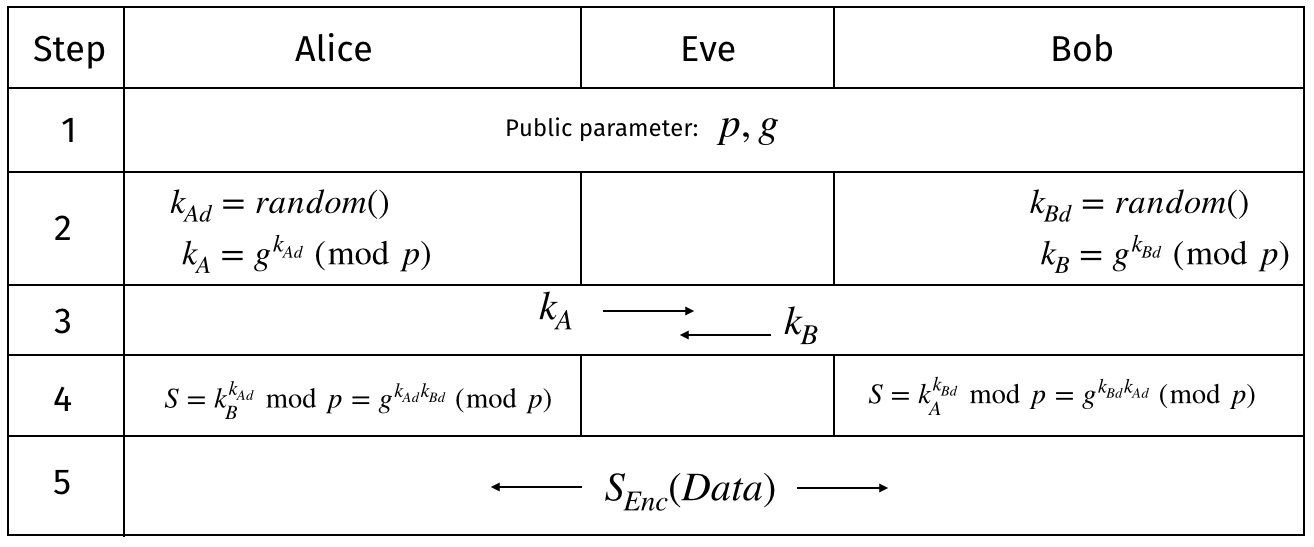
\includegraphics[width=.9\linewidth, height=.67\textheight, keepaspectratio]{Figures/DHKE}
	\caption{Exchanging shared secret key using DH-key exchange.}
	\label{fig_DHKE}
\end{figure}

Rivest, Shamir, and Adleman (RSA) realized this protocol in 1977 and published their magnum opus which is widely known as RSA cryptosystem \cite{rivest1978method}. 
The security of the RSA depends on the difficulty of factorization of a larger integer into its two prime factors and the trapdoor permutation for encryption.
Let us denote two large primes $p$ and $q$ (in practice about 1000-bit).
It is easy to calculate their product to get $n = pq$.
The reverse process that is for a given integer $n$ it will be arduous to retain $p$ and $q$.
Using the state-of-the-art integer factoring algorithm \textit{general number field sieve }(GNFS), it will take approximately $2^{90}$ basic operation to factor a 2048-bit integer.
After more than 40 years of the RSA breakthrough, it is still standing as an epitome of public key cryptography.
Besides encryption, RSA also enables \textit{digital signature }where the sender uses his private key to sign a message, and the receiver verifies the signature by the senders public key. 
Verification of a digitally signed message gives the receiver the confidence that a senders private key is tied to his public key.
It is done to prevent forgery and holds \textit{Non-repudiation} property.

In the mid 80's the independent work of Miller \cite{C:Miller85} and Koblitz \cite{koblitz1987elliptic} began the journey of elliptic curve cryptosystems (ECC). 
The security of elliptic curve cryptography protocols depends on the difficulty to solve elliptic curve discrete logarithm problem.
The mathematical details of this problem appear in Chapter 2. %TODO
ECC provides a shorter key length for the same level of security than RSA which makes ECC  popular among the researchers. 
Compared to RSA, ECC has other advantages. 
While RSA provides encryption and digital signature; ECC has a family of algorithms for encryption, signature, key agreement and some advanced high-level cryptographic protocols such as ID-based encryption \cite{AC:BonLynSha01}, where user's unique ID, e.g. email address, can be used as a public key. 
The high-level cryptographic functionalities are provided by paring over elliptic curves \cite{book_GPCMrabet2016} which brings a new paradigm in cryptography called pairing-based cryptography.

\subsection{Pairing-Based Cryptography}
\label{ch1_subsec_pbc}
Since the inception by Sakai et al. \cite{sakai2000cryptosystems}, pairing-based cryptography has gained much attention to cryptographic researchers as well as  to mathematicians. It gives flexibility to protocol researcher to innovate applications with provable security and at the same time to mathematicians and cryptography engineers to find efficient algorithms to make pairing implementation more efficient and practical.

Generally, a pairing is a bilinear map $e$ typically defined as  $\g1 \times \g2 \to \g3$, where $\g1$ and $\g2$ are additive cyclic sub-groups of  order $r$  on a certain elliptic curve $E$ over a finite extension field $\FPK$ and $\g3$ is a multiplicative cyclic group of order $r$ in $\mF{p}{k}$.
Let $E(\Fp)$ be the set of rational points over the prime field $\Fp$ which forms an additive Abelian group together with the point at infinity $\cal{O}$. The total number of rational points is denoted as $\#E(\Fp)$. Here, the order $r$ is a large prime number such that $r | \#E(\Fp)$ and gcd$(r,p)=1$. The embedding degree $k$ is the smallest positive integer such that $r | (p^k -1)$.
Two fundamental properties of pairing are
\begin{itemize}
	\item bilinearity is such that $\forall P_i \in \g1$ and $\forall Q_i \in \g2$, where $i= 1, 2$, then $e(Q_1+Q_2,P_1) = e(Q_1,P_1). e(Q_2,P_1)$ and $e(Q_1,P_1+P_2) = e(Q_1,P_1). e(Q_1,P_2)$,
	\item and $e$ is non-degenerate means $\forall P \in \g1$ there is a $Q \in \g2$ such that  $e(Q,P) \neq 1$ and $\forall Q \in \g2$ there is a $P \in \g1$ such that $e(P,Q) \neq 1$.
\end{itemize}
Such properties allows researchers to come up with various cryptographic applications including ID-based encryption \cite{C:BonFra01}, group signature authentication \cite{C:BonBoySha04}, and functional encryption \cite{C:OkaTak10}.  However, the security of pairing-based cryptosystems depends  on 
\begin{itemize}
	\item  the difficulty of solving elliptic curve discrete logarithm problem (ECDLP) in the groups of order $r$ over $\Fp$,
	\item  the infeasibility of solving the discrete logarithm problem (DLP) in the multiplicative group $\g3 \in \mF{p}{k}$,
	\item and the difficulty of pairing inversion.
\end{itemize}
To maintain the same security level in both groups, the size of the order $r$ and extension field $p^k$ is chosen accordingly. If the desired security level is $\delta$ then $\log_2 r  \geq 2\delta$ is desirable due to Pollard's rho algorithm \cite{1978-pollard-kangaroo}.  For efficient pairing, the ratio $\rho = \log_2 p^k/ \log_2 r \approx 1$,   is expected (usually  $1\leq  \rho  \leq 2$). In practice, elliptic curves with small embedding degrees $k$ and large $r$ are selected and commonly are knows as ``pairing-friendly" elliptic curves.

Galbraith et al. \cite{galbraith2008pairings} have classified pairings as three major categories based on the underlying group's structure as 
\begin{itemize}
	\item Type 1, where $\g1 = \g2$, also known as symmetric pairing. 
	\item Type 2, where $\g1 \neq \g2$, known as asymmetric pairing. There exists an efficiently computable isomorphism $\psi : \g2 \to \g1$ but none in reverse direction.
	\item Type 3, which is also asymmetric pairing, i.e., $\g1 \neq \g2$. But no efficiently computable isomorphism is known in either direction  between $\g1$ and $\g2$.
\end{itemize}


%This thesis chooses one of the Type 3 variants of pairing named as Optimal-Ate \cite{DBLP:journals/tit/Vercauteren10} with Kachisa-Schaefer-Scott (KSS) \cite{EPRINT:KacSchSco07} pairing-friendly curve of embedding degree $k=16$. 
%Few previous works have been done on this  curve. 
%Zhang et al. \cite{INDOCRYPT:ZhaLin12} have shown the computational estimation of the Miller's loop and proposed efficient final exponentiation for 192-bit security level in the context of Optimal-Ate pairing over KSS-16 curve. 
%A few years later Ghammam et al. \cite{EPRINT:GhaFou16b} have shown that KSS-16 is the best suited for multi-pairing (i.e., the product and/or the quotient) when the number of pairing is more than two. 
%Ghammam et al. \cite{EPRINT:GhaFou16b} also corrected the flaws of proposed final exponentiation algorithm by Zhang et al. \cite{INDOCRYPT:ZhaLin12} and proposed a new one and showed the vulnerability of Zhang's parameter settings against small subgroup attack. 
%The recent development of NFS by Kim and Barbulescu \cite{C:KimBar16} requires updating the parameter selection for all the existing pairings over the well known pairing-friendly curve families such as BN \cite{SAC:BarNae05}, BLS \cite{EPRINT:FreScoTes06} and KSS \cite{EPRINT:KacSchSco07}.
%The most recent study by Barbulescu et al. \cite{EPRINT:BarDuq17} have shown the security estimation of the current parameter settings used in well-studied curves and proposed new parameters, resistant to small subgroup attack.
%
%Barbulescu and Duquesne's study finds that the current parameter settings for 128-bit security level on BN-curve studied in literature can withstand for 100-bit security. 
%Moreover, they proposed that BLS-12 and surprisingly KSS-16 are the most efficient choice for Optimal-Ate pairing at the 128-bit security level. Therefore, the authors focus on the efficient implementation of the less studied KSS-16 curve for Optimal-Ate pairing by applying the most recent parameters.
%Mori et al. \cite{PAIRING:MANS13} and Khandaker et al. \cite{ICISC:KONSD16} have shown a specific type of sparse multiplication for BN and KSS-18 curve respectively where both of the curves supports sextic twist. 
%The authors have extended the previous works for quartic twisted KSS-16 curve and derived pseudo-8 sparse multiplication for line evaluation step in the Miller's algorithm. 
%As a consequence, the authors made the choice to concentrate on Miller's algorithm's execution time and computational complexity to verify the claim of \cite{EPRINT:BarDuq17}.
%The implementation shows that Miller's algorithm time has a tiny difference between KSS-16 and BLS-12 curves. However, they both are more efficient and faster than BN curve. 
\section{Motivation}
\label{ch1_sec_motivation}

This section outlines the overall motivation behind the undertaken works.
In this course, some mathematical notations will appear without detailed definitions.
The subsequent chapters will define them with further elaboration.
Let us consider the following two cases.

\subsection*{Case 1: IoT Security}
Human civilization is moving to a direction where data generated from the devices used in our daily life will define how smart our society will be.
In technical jargon, we define that IoT (Internet of Things) era controlled by Data Science.
Some data can be mundane with no purpose, and some data can be extraordinarily important.
Let us imagine a case where the adversary takes controls heartbeat monitor sensor of our smartwatch or control sensors of a self-driving car.
The outcome of the damage is unimaginable. 
There is no alternative to protect these data from unwanted access.
The challenge is, most of the IoT devices are equipped with small sensors.
Such devices are computationally resource constrained.
In some devices, it is somewhat impractical to generate key pairs for widely practiced security protocols.
There are several innovative solutions such as Identity-based encryption that can use device's unique ID as a key.
The applications mentioned above stand on a compelling branch of cryptography named \textit{pairing-based cryptography over elliptic curve}.


\subsection*{Case 1: Security of Medical Data in Cloud}
Modern medical diagnosis depends on medical examination that produces a vast amount of data ranges from patients personal information to diagnosis reports and images.
Most of the data are stored in large cloud-based databases. 
For the privacy of the patient, they should be encrypted before stored.
By analyzing such medical data, it is possible to predict the probability of a patient's vulnerability to a particular disease. 
However, it is not always the doctor who examined the patient can do that.
Sometimes third-party researchers are interested in such data-set. 
However, the identity of the patient should not be obtained by any third-party using that data. 
One solution for this case is any third party can search data and perform the mathematical operation in the encrypted database without decrypting the data.
This scenario can be realized by using homomorphic encryption which is also powered by pairing-based cryptography.

However, pairing-based cryptography is a complex mathematical process.
To practically apply it, we need to carry out its fundamental algorithms more efficiently.
In this thesis, our objective is to improve and find out more efficient algorithms that can realize high-level of security protocols.

\section{Our Contribution}
\label{ch1_sec_contribution}
As discusses above, pairing is a bilinear map from two groups $\mathbb{G}_1$ and $\mathbb{G}_2$ to a group $\mathbb{G}_3$, where they have respectively same prime order $r$.
In detail, $\mathbb{G}_1$ and $\mathbb{G}_2$ respectively becomes a subgroup in an elliptic curve group $E(\F{q}{})$ and $E(\F{q}{k})$, and $\mathbb{G}_3$ becomes a subgroup in $\F{q}{k}$, where $q$ is a power of $p$ and an extension degree $k$ is especially called the {\it embedding degree}.

In pairing-based cryptography, there exists several predominant operations which are the bottleneck for any pairing-based protocols.
These operations are Miller's algorithm, final exponentiation in $\mathbb{G}_3$, scalar multiplications in $\mathbb{G}_1$ and $\mathbb{G}_2$, and exponentiation in $\mathbb{G}_3$.
The calculation costs of pairing and scalar multiplication in $\g{2}$ are the significant costs among the operations required for pairing-based cryptographies.
Therefore, efficient Miller's algorithm and scalar multiplications in $\mathbb{G}_2$ can reduce the total cost of pairing-based cryptography.
In this work, we focus on these operations especially Miller's algorithm and scalar multiplications in $\mathbb{G}_2$.
	
In this thesis, we focus on Type 3 pairing that is asymmetric pairing such as Ate \cite{EPRINT:MKHO07} and Optimal-Ate \cite{DBLP:journals/tit/Vercauteren10} pairing.
Therefore, we have not efficient homomorphic map from $\g{1}$ to $\g{2}$. 
Generally, in asymmetric pairing the scalar multiplication is carried out over efficiently calculable group $\g{1}$ and then the result is mapped to $\g{2}$.

The {\it embedding degree} is an important parameter that determines the security level of pairing-based cryptographies.
Therefore, to achieve efficient pairing on ordinary curves whose {\it embedding degree} are flexibly selectable are required.
This thesis targets Ate and {\it twisted} Ate pairings because they are efficiently calculated on normal pairing-friendly curve Kachisa-Schaefer-Scott (KSS) \cite{EPRINT:KacSchSco07}.
Ate and Optimal-Ate are use calculated over certain elliptic curve groups $\g{1}$ and $\g{2}$.
In this thesis, we accelerate scalar multiplications in $\g{2}$ group which can be extended in $\g{1}$

In the case of scalar multiplication, we reduce the number of elliptic curve doubling by decomposing a scalar with a key relation for KSS curves.
Besides, we proposed state-of-the-art Miller's algorithm calculation at the 128-bit security level.

Our proposed methods can substantially improve pairing calculation.
Therefore, our research contributes to committing high-level security for sophisticated protocols, e.g. ID-based or Homomorphic encryption.

\section{Thesis Outline}
\label{ch1_sec_outline}
This thesis is organized as follows: 

In Chapter 2, we briefly discuss the mathematical concepts that are related to understanding the concepts of this thesis.
We also define the pairing in general. 
Besides, a target class of pairing-friendly elliptic curves is shown.

Chapter 3 proposes an efficient Optimal-Ate pairing for KSS-18 curve. 
We improved the Miller's algorithm of Optimal-Ate pairing by proposing \textit{pseudo 12-sparse multiplication} multiplication.
In order to evaluate our theoretic proposal, we also include some experimental results with recommended parameter settings.

Chapter 4 proposes a technique that will accelerate scalar multiplications in $\g{2}$ over KSS-18 curve. 
It is crucial to derive efficiently computable endomorphisms for accelerating scalar multiplication.
The target $\g{2}$ group has a property that specific scalar multiplication can utilize  Frobenius endomorphism that is efficiently computable.
Focusing on this property, we derive an essential relation available for scalar multiplication in $\g{2}$ from the structural properties of target elliptic curve.
Then, using the relation, efficient scalar multiplication is proposed together with multi-scalar multiplication.
Besides, from the experimental results, we show that the proposed scalar multiplication is about 60 times faster than the conventional method.  

In chapter 5, we derived twist property for target elliptic curves for 192-bit security level and compared their performances concerning scalar multiplication.
This thesis shows that sextic twist over KSS-18 curve has an advantage over quartic twist in KSS-16 curve.

Chapter 6, shows the state-of-the-art improvement of Optimal-Ate pairing over KSS-16 curve at the 128-bit security level.
We adopted the most recent parameter and theoretically derived most efficient pairing calculation.
Besides, we also showed experimental implementation and compared our result with other pairing-friendly curves.


In Chapter 7, we opt to further accelerate the work of chapter 6 by improving the finite field arithmetic using cyclic vector multiplication algorithm.
We showed comparative results between chapter 6's proposal and this. 
We also showed memory optimization currently exists final exponentiation algorithm.

Chapter 8 shows the   $\g{2}$  scalar multiplication with by applying different dimension of GLV decomposition.
We showed theoretical and experimental result and showed that 4-dimension is optimal for efficient scalar multiplication in  $\g{2}$ in KSS-16 curve.

Finally, Chapter 9 concludes this thesis.

	


\chapter{Fundamental Mathematics and Notation}
\label{chap:fundamentals} 
It is necessary to recall some fundamental mathematical concept to understand the subsequent chapters and introduce the notations used in the thesis.
This chapter introduces the essential mathematical backgrounds that are directly relevant to the contents of this thesis to help readers to a clear understanding of the subsequent chapters.
The theoretical discussion will often appear with minimal definition and citation of the details works since details discussion is beyond the scope of this thesis.
For more details of the topics discussed in this chapter we refer to \cite{lidl_niederreiter_1996, book_HFFMullen2013}.
As an additional purpose, this chapter specifies most of the notations that will appear in the upcoming chapters.
% For referencing the chapter elsewhere, use \ref{Chapter1} 

Cryptography deals with numbers mostly integers.
To understand modern cryptography  it is essential to have a good understanding of the  underlying mathematical concepts. 
The following concepts is the basic for the discussion of the subsequent chapters.

\section{Modular Arithmetic}
\label{sec:chap:fund:modular_arithm} 
 Modular arithmetic is the fundamental tool for modern cryptography specially public key cryptosystems.
\begin{definition}[Modular Arithmetic\index{modulus}]
	Let  $p$ be a positive integer named as the modulus \index{modulus} and  $a$ and $b$  are two arbitrary integers. 
	If  $p$ divides $b-a$  then we can write
	 $$ a \equiv b ~(\bmod ~p)$$
	 and express as $a$ and $b$ are congruent modulo $p$.
\end{definition}
\begin{example}
	Let, $p =7$, $a=19$ and $b=5$ then 
	$19  \equiv  5 ~(\bmod ~7) $.
\end{example}

\begin{example}
	Let, $p =7$, $a=-17$  and $b=11$. Then $-17  ~(\bmod ~7)  = 4$ and $11 ~(\bmod ~7) = 4$. 
	We can write 
	$$-17  \equiv  11 ~(\bmod ~7) $$ 
	and usually express $-17$ and $11$ are congruent modulo $7$.
\end{example}

\section{Group, Ring, Field}
\label{sec:chap:fund:group}
\subsection{Group}
The concept of group \index{group} is very fundamental for understanding cryptography. It is an algebraic system defined as follows.
\begin{definition}[Group\index{group}]
A group \index{group} is a non empty set $\mathbb{G}$ with a binary operation $\circ$ on its elements denoted as  $\langle\mathbb{G}\index{group},\circ\rangle$,  sometimes denoted by   $\mathbb{G}$ only, which satisfies the following axioms.
\begin{quote}
	\begin{description}
		\item[Closure] The group is closed under the operation $\circ$, i.e.  $\forall a \in\mathbb{G}$, and $\forall b \in\mathbb{G}$ the result of $ (a\circ b) = c \in \mathbb{G}$. \footnote{$\forall$ symbol bears is usual notation \textit{"for all"} }
		
		\item[Identity element] There exist an \textbf{identity element \index{Identity element}} $e$ also know as \textit{neutral element} or \textit{unit element} in $\mathbb{G}$ such that $\forall a \in\mathbb{G} \index{group}$,  $a\circ e = e\circ a = a$.
		
		\item[Inverse element] For ${\forall}a \in\mathbb{G}\index{group}$, there exists an element $b\in\mathbb{G}\index{group}$ such that $a\circ b=e=b\circ a$, where $b$ is called inverse element of $a$.
		
		\item[Associativity] Elements in  group $\mathbb{G}$ should follow associativity. i.e. $(a\circ b)\circ c=a\circ (b\circ c)$ for all $ a,b,c\in\mathbb{G}\index{group}$.
		
\end{description}
\end{quote}
\end{definition}

\begin{definition}[Commutative Group\index{group}] \hspace{0em}
\begin{quote}\begin{description}
A group \index{group} $\mathbb{G}\index{group}$ will be commutative if $a\circ b=b\circ a$ for all $a,b \in\mathbb{G}\index{group}$.
\end{description}\end{quote}
\qed
\end{definition}
A commutative group is also called \textit{abelian} group.

\begin{example} \label{example_group}
 The set of integers $\mathbb{Z}$ forms a group under the group operation of addition $+$ denoted as $(\mathbb{Z},+)$. $0$ is the identity element of the group.
\end{example}
\begin{example}\label{example_notgroup}
	 The set of positive integers $\mathbb{N}$ under addition does not form a group since elements have not inverse.
\end{example}
%For example, the algebraic system $\langle\mathbb{Z},+\rangle$ is an infinite commutative group\index{group}, where $\mathbb Z$ is the integer set and $+$ means the ordinary addition for integers. For a finite group\index{group}, its order\index{group order} is defined as follows.
\begin{definition}[Order of a Group\index{group}]\hspace{0em}
The order of a group $\mathbb{G}$ \index{group order} often denoted as $\#\mathbb{G}\index{group}$ is the number of elements in the group\index{group} $\mathbb{G}\index{group}$.
\qed
\end{definition}

\begin{remark}
	 Groups order can be finite and infinite. In example \ref{example_group}, $(\mathbb{Z},+)$ has infinite order.
\end{remark}

\begin{definition}[Order of group element\index{order of element}]
	For an element $a\in\mathbb{G}\index{group}$, the smallest positive integer $m$ such that $a^{m}=e$ is called the order\index{order} of $a$, where $e$ is the identity element in $\mathbb{G}\index{group}$.
	\qed
\end{definition}

\begin{example}{Finite group:  \index{finite group} } \label{definition_finite_group}
As shown in example \ref{example_notgroup}, the set $\mathbb{N}$ under addition does not form a group 
since it does not satisfy the group\index{group} axioms. 
Let us consider a set $\mathbb{N}_{n}$ under the operation $\mod n$  such that 
$$ \mathbb{N}_{n} = \{0,1,2,3, \cdots, n-1\}$$
where $n \in \mathbb{N}$.
It means $\mathbb{N}_{n}$ is the set of remainders under ``$\bmod\ n$''.
Recall the modular arithmetic that 
$$a+b\equiv c\ \ \bmod n\hspace{3em}a,b\in \mathbb{N}_{n},\label{Sum Definition}$$
 means $c$ is  associated to a remainder on division by $n$ when $a+b=c\notin\mathbb{N}_{n}$. 
It makes $c$ belongs to $\mathbb{N}_{n}$ making $( \mathbb{N}_{n},+)$ forming a group\index{group}.
In also includes element $0$ which acts as an identity element.
\end{example}

\begin{definition}[Group generator\index{group}]
	For a given group\index{group} $\mathbb{G}\index{group}$ if there is an element $g\in\mathbb{G}\index{group}$ such that for any $a\in\mathbb{G}\index{group}$ there exist an unique integer $i$ with $a=g^{i}$ then $g$ will be called a   generator\index{generator} of  $\mathbb{G}\index{group}$
\qed
\end{definition}

\begin{definition}[Cyclic Group\index{group}]
A group\index{group} $\mathbb{G}\index{group}$ will be {\em cyclic} if there exist at least one generator $g \in \mathbb{G}$. Cyclic group usually expressed as $\mathbb{G} = \langle g \rangle$
 \qed 
\end{definition}

\begin{remark}
	The number of generator in a group $\mathbb{G}\index{group}$ of order $n$ is defined by Euler's totient function $\phi(n)$\footnote{When $n$ is a positive integer, Euler's totient function $\phi(n)=$ number of positive integers less than or equal to $n$ that are co-prime to $n$}.
	If $n$ is a prime $p$ then the  group $\mathbb{G}$ will be called prime order group and it will have $\phi(p) = p-1$ generators.
\end{remark}

\begin{definition}[Cyclic Group\index{group}]
	A group\index{group} $\mathbb{G}\index{group}$ will be {\em cyclic} if there exist at least one generator $g \in \mathbb{G}$. Cyclic group usually expressed as $\mathbb{G} = \langle g \rangle$ 
	\qed 
\end{definition}

In this case we use the notation $\langle\mathbb{G}\index{group},\circ\rangle$,  there exists some ambiguity which operation we consider.
Therefore, the following two types of group nations are very common in literature.

\begin{definition}[Additive group\index{additive group}]
A cyclic group is called \textit{additive} if we tend to write its group operation in the same way we do additions, that is 
$$f = g + x$$ 
can also appear as $[x]g$ meaning applying $x -1$ times addition operator $+$ on $g$.
It is also common to write as $x \cdot g$.
For example, $1$ is one of generators in group $(\mathbb{Z}_5, + )$ under addition modular $5$, then $1 \cdot 4$ can be written as $$ 4 = 1+ 1+ 1+1.$$
\qed
 \end{definition}

\begin{definition}[Multiplicative group\index{multiplicative group}]
	A cyclic group is called \textit{multiplicative} if we tend to write its group operation in the same way we do multiplication, that is 
	$$f =  g \cdot x ~\text{or}~ f = g^x$$ 
	\qed
\end{definition}

\begin{remark}
	In both notation the $x$  is an integer called the \textit{discrete logarithm} of $h$ to the base $g$.
\end{remark}
\begin{remark}
	Unless otherwise stated, through out this thesis we will use the $xg$ notation for ordinary addition e.g. $a+a=2a$ and $a+a+a=3a$ and for multiplicative notation, these will denoted by $a^2$, $a^3$.
\end{remark}

From the definition cyclic group, it can be see visualized that any elements in cyclic a group\index{cyclic group} are generated with iterative operations of generator\index{generator} $g$. 
\fgref{Cyclic group} shows this schematically.
\begin{figure}[ht]
\begin{center}
	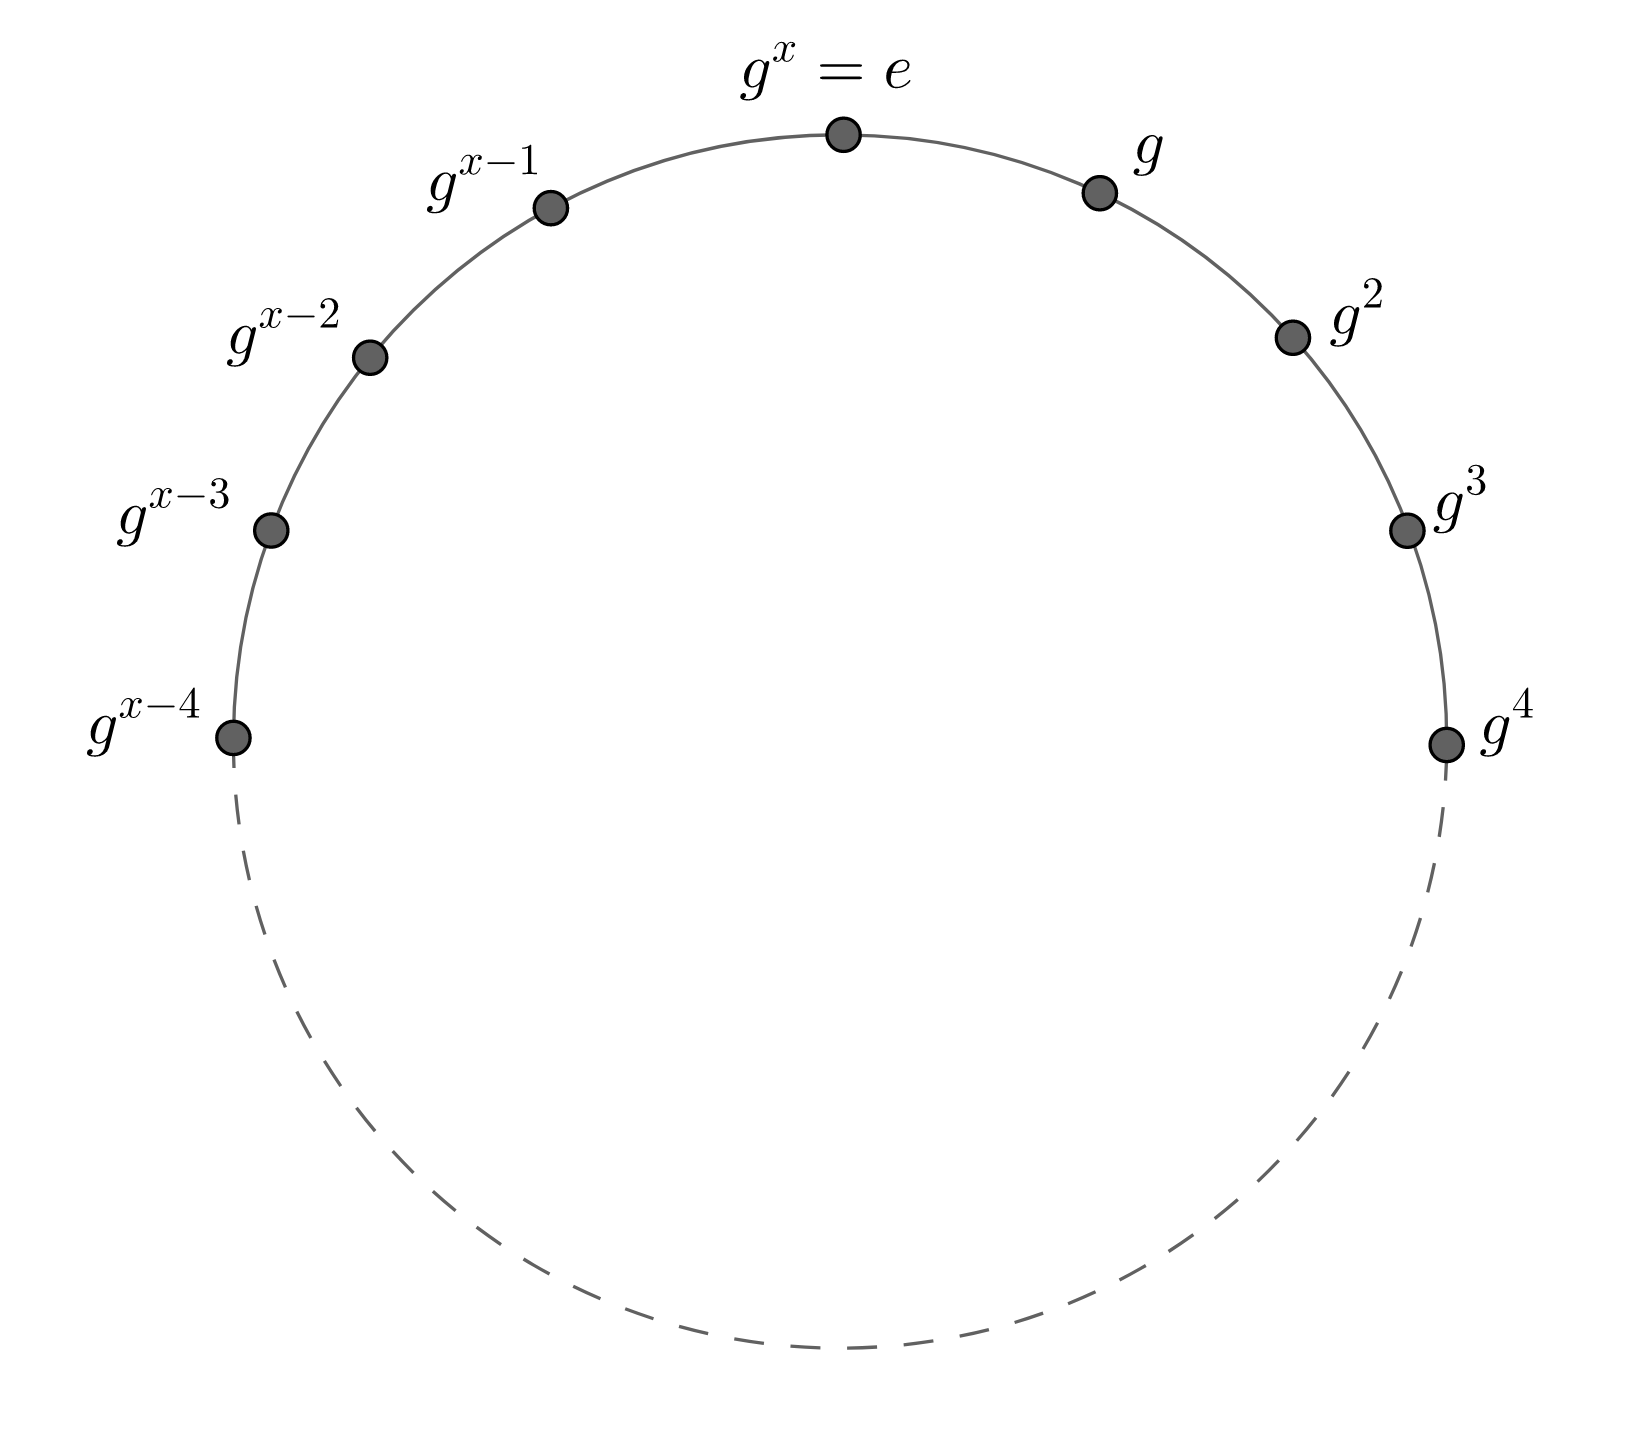
\includegraphics[width=.6\linewidth, height=.67\textheight, keepaspectratio]{Figures/cyclicgroup}
\caption{Cyclic group\index{cyclic group}\index{group}}
\label{Cyclic group}
\end{center}
\end{figure}

A a well known practice of presenting a finite group's\index{group} operation is {\em Cayley table\index{Cayley table}} as shown in example \ref{example_Cayleytable}.
Cayley table\index{Cayley table} shows all possible group operation that can be performed in a finite group.

\begin{example} \label{example_Cayleytable}
	The Cayley table\index{Cayley!Cayley table} for the group\index{group} $\mathbb{Z}_4$ is:
	\begin{center}
		\begin{tabular}{c|cccc}
			$\oplus_4$&\em 0&\em 1&\em 2&\em 3       \\
			\hline
			\em 0&\em 0&\em 1&\em 2&\em 3       \\
			\em 1&\em 1&\em 2&\em 3&\em 0       \\
			\em 2&\em 2&\em 3&\em 0&\em 1       \\
			\em 3&\em 3&\em 0&\em 1&\em 2       \\
		\end{tabular}
	\end{center}
\end{example}
In the above example of group $(\mathbb{Z}_4,+)$, there are $\phi(4)=2$ generators, $3$ and $1$.

\begin{definition}[Subgroup\index{subgroup}]
	Let $\mathbb{H}$ be  a non-empty subset  fo group $\mathbb{G}$, $\mathbb{H}$  will be called subgroup of $\mathbb{G}$ if  $\mathbb{H}$  itself follows group axioms and $\mathbb{H}$ has the same identity element of group $\mathbb{G}$. 
	\qed
\end{definition}

\begin{theorem}[Lagrange's Theorem:]
	Let $\mathbb{G}$ be a finite abelian group and $\mathbb{H}$ is a subgroup of $\mathbb{G}$.  The order of $\mathbb{G}$, $\#\mathbb{G}$ is divisible by the order of subgroup $\mathbb{H}$, $\#\mathbb{H}$ i.e.   $\#\mathbb{H} | \#\mathbb{G}$.
\qed
\end{theorem}

\begin{theorem}[Fermat’s Little Theorem:]
	Let $p$ is a prime and $a \in \mathbb{Z}$, then $$a^p = a ~(\bmod ~p)$$
	\qed
\end{theorem}
Fermat’s \textit{little theorem} is a special case of Lagrange’s theorem.


\subsection{Homomorphism in groups \index{homomorphism}}
Morphisms in groups is often used the research of cryptography and inseparable to for pairing-based cryptography research.
\begin{definition}[Homomorphism\index{rings}]
	Let $(\mathbb{G},\circ)$ and $(\mathbb{G}^{'},\star)$ be two groups with identity elements $e$ and $e'$ respectively.
	A homomorphism  is a map $f$ which preserves the group structure while the elements are mapped from $(\mathbb{G},\circ)$ to $(\mathbb{G}^{'},\star)$.
	\qed
\end{definition}
	A homomorphic map obeys the following conditions:
	\begin{itemize}
		\item $\forall a,b \in \mathbb{G}$, $f(a \circ b) = f(a) \star f(b)$.
		\item  For every $a \in \mathbb{G}$, the inverse map is $f(a^{-1}) = f(a)^{-1}$.
		\item  Identity element mapping also preserves the structure i.e. $f(e) =e'$.
	\end{itemize}

\subsubsection{Types of Homomorphism}
\begin{quote}
	\begin{description}
				\item[Isomorphism \index{Isomorphism}] If element from $\mathbb{G}$  and $\mathbb{G}^{'}$ have bijective relation then $\mathbb{G}$ and $\mathbb{G}^{'}$ are isomorphic to each other.
					
			\item[Endomorphism  \index{Endomorphism}]  If elements from group $(\mathbb{G},\circ)$ is mapped to itself then it is called endomorphism. 
			A frequently used endomorphism in cryptographic algorithms is Frobenius endomorphism. 
			
			\item[Authomorphism  \index{Authomorphism}] If element of a group has both endomorphism and isomorphism then it is called automorphism.
	\end{description}
\end{quote}

\begin{definition}[Kernel\index{kernel}]
	Let $(\mathbb{G},\circ)$ and $(\mathbb{G}^{'},\star)$ be two groups with identity elements $e$ and $e'$ respectively and $f$ is homomorphism from $(\mathbb{G},\circ)$ to $(\mathbb{G}^{'},\star)$.
	The kernel of $f$ is denoted as $\text{Ker}\{f\}$, defined by 
	$$\text{Ker}(f) = \{ a \in \mathbb{G}: f(a) = e'\}$$.
	\qed
\end{definition}

%--------------------------------------
%--------------------------------------
\subsection{Ring}
The concept of \textit{Ring} will not come as frequently as group and field in the subsequent chapters. 
However, it is relevant to define ring to understand the related concept.
\begin{definition}[Ring \index{ring}]
	A \textbf{ring} $\mathbb{R}$ is an algebraic structure with two operations, i.e. addition  $+$ and  multiplication $\cdot$  usually denote as $\mathbb{R},+,\cdot$.
	\begin{itemize}
		\item $\mathbb{R}$ is abelian group under addition operation.
		\item Under multiplication, $\mathbb{R}$ is closed and associative with identity element is $1$.
		\item  Multiplication is distributive over addition: $ \forall a, b, c \in \mathbb{R}: a\cdot (b+c) = a\cdot b + a\cdot c$.
	\end{itemize}
\qed
\end{definition}
If multiplication operation is commutative, $\mathbb{R}$  forms a commutative ring.
%\begin{example}
%	TODO
%\end{example}
\begin{definition}[Multiplicative Inverse Modulo $n$ \index{multiplicative inverse}]
	Let $\mathbb{Z}_n$ be a set under modulo $n$ and $a \in \mathbb{Z}_n$. 
	The multiplicative inverse modulo $n$ of $a$ can be written as  follows:
	$$a\cdot x \equiv  1 \bmod n.$$
The value $x$ is the multiplicative inverse modulo $n$ of $a$, often written as $a^{-1}$.
\qed
\end{definition}
Such value of $x$ only exists if $\text{gcd}(x,n)=1$.
If $n=p$ is a prime then every non-zero element in the set $\mathbb{Z}_p$ will have multiplicative inverse.
Such $(\mathbb{Z}_p,+,\cdot)$ will be a ring and having the above property it will form a field.

\subsection{Field}
\begin{definition}[Field]
	A field $(\f{},+,\cdot)$ is a set that obeys two binary operations denoted by $+$ and $\cdot$, such that:
	\begin{itemize}
%		\begin{itemize}
			\item $\f{}$ is a commutative group with respect to $+$ having identity element $0$.
			
			\item Let ${\f{\,}}^{\ast}\!\!$ is a subset of $\f{}$ having only not-zero element of $\f{}$ i.e. ${\f{}}^{\ast}  = {\f{} ~\backslash \{0\}}$. 
			Then ${\f{\,}}^{\ast}\!\!$ will be called a commutative group respect to multiplication$\cdot$  where every element should have multiplicative inverse in  ${\f{\,}}^{\ast}\!\!$.
			\item For all $a,b,c \in\f{}$  the distributive law will be followed, e.g. $a\cdot(b+c)=a\cdot b+a\cdot c$ and $(b+c)\cdot a=b\cdot a +c\cdot a$.
	\end{itemize}
%\end{itemize}
	\qed
\end{definition}
%In general, the elements $0$ and $1$ denote the unit elements regarding to addition $+$ and multiplication $\cdot$, respectively.
\begin{definition}[Subfield \index{subfield}]\hspace{0em} \label{definition_subfielf}
	Let $\f{1}$ is a subset of field $\f{}$. $\f{1}$ will be called a subfeld if $\f{1}$ itself obeys the laws of field with respect to the field operation inherited from  $\f{}$.
	\qed
\end{definition}
\begin{remark}
	 In Definition \ref{definition_subfielf}, $\f{}$ is called an {\em extension field} of $\f{1}$.
	  If $\f{1}\neq \f{}$, then $\f{1}$ is a {\em proper subfield} of $\f{}$.
 \end{remark}

\begin{definition}[Order of Finite Field \index{order of field}]\hspace{0em}
	The order is the number of elements in $\f{}$. If the order of $\f{}$ is finite, $\f{}$ is called finite field. 
	\qed
\end{definition}
\begin{definition}[Characteristic of Finite Field \index{field characteristics}]\hspace{0em}
	Let $\f{}$ be a field and smallest positive number $n$ such that $n \cdot a= 0$ for every $a\in \f{}$. Such $n$ is called characteristic. If there is no such $n$ in  $\f{}$ then $\f{}$ has characteristics $0$.
	\qed
\end{definition}

Most of the works presented in this dissertation deals with  finite fields only. 
A common property of finite fields often used in cryptographic is fllows:
\begin{theorem}\label{Cyclic Group in Finite Field}
	For every finite field $\f{}$, the multiplicative group $({\f{\,}}^{\ast}\!\!, \cdot)$ is cyclic. 
	\qed
\end{theorem}
%For example, ElGamal encryption \cite{C:ElGamal84} can be defined over multiplicative group of $\f{}$. Its security depends on the difficulty of a problem in $\f{}$ related to computing {\em discrete logarithms}.
%A subset $\mathbb K$ of a field $\f{}$ that is itself a field under the operations of $\f{}$ will be called a {\em subfield} of $\f{}$. In this case, $\f{}$ is called an {\em extension (field)} of $\mathbb K$. If $\mathbb K\neq \f{}$, we say that $\mathbb K$ is a {\em proper subfield} of $\f{}$. Then, {\em prime field} is defined as follows.
\begin{definition}[Prime Field \index{prime field}]
	Let $p$ be a prime. The ring of integers modulo $p$ is  a finite field of characteristics $p$ having field order $p$ denoted as $\f{p}$ is called a prime field.
	 \qed
\end{definition}
\begin{remark}
		A prime field contains no proper subfield.
\end{remark}

\begin{theorem}
	Every finite field has a prime field as a subfield. \qed
\end{theorem}

In this work we classified finite fields into two types, i.e.  prime field $\f{p}$ and its extension field. 
Defined \ref{sec:chap:fund:extenion_field} explains more of extension field.
The prime field $\Fp$ has  the order and characteristic as $p$.
Using the modular arithmetic in the same way as Definition \ref{sec:chap:fund:extenion_field}, we can define fundamental operations of prime field $\Fp=\{0,1,2\cdots,p-1\}$.
The Cayley table will de
\begin{example}The Cayley table for the two operations $+$ and $\cdot$ for elements in $\f{5}$ are as follows:
	\begin{center}
		\begin{tabular}{c|ccccc}
			$+$&\em 0&\em 1&\em 2&\em 3&\em 4       \\
			\hline
			\em 0&\em 0&\em 1&\em 2&\em 3&\em 4       \\
			\em 1&\em 1&\em 2&\em 3&\em 4&\em 0      \\
			\em 2&\em 2&\em 3&\em 4&\em 0&\em 1      \\
			\em 3&\em 3&\em 4&\em 0&\em 1&\em 2      \\
			\em 4&\em 4&\em 0&\em 1&\em 2&\em 3      \\
		\end{tabular}\ \ 
		\begin{tabular}{c|ccccc}
			$\cdot$&\em 0&\em 1&\em 2&\em 3&\em 4       \\
			\hline
			\em 0&\em 0&\em 0&\em 0&\em 0&\em 0       \\
			\em 1&\em 0&\em 1&\em 2&\em 3&\em 4      \\
			\em 2&\em 0&\em 2&\em 4&\em 1&\em 3      \\
			\em 3&\em 0&\em 3&\em 1&\em 4&\em 2      \\
			\em 4&\em 0&\em 4&\em 3&\em 2&\em 1      \\
		\end{tabular}
	\end{center}
\end{example}
As described above, we can define arithmetic operations in $\Fp$ by modular operations ($\bmod\ p$) for integers. However, it does not work in an extension field $\F{p}{m}$. In the next section, arithmetic operations in extension field $\F{p}{m}$ is described in detail.


\section{Extension Field} 
%\label{sec:chap:fund:extenion_field}
\label{sec:chap:fund:extenion_field}
%--------------------------------------
A subset $\F{0}{}$ of a field $\F{}{}$ that is itself a field under the operations of $\F{}{}$ will be called a {\it subfield} of $\F{}{}$.
In this case, $\F{}{}$ is called an {\it extension field} of $\F{0}{}$.
An extension field of a prime field $\F{p}{}$ can be represented as $m$-dimensional vector space that has $m$ elements in $\F{p}{}$.
Let the vector space be the $m$-th extension field, it is denoted by $\F{p}{m}$.
The order of extension fields $\F{p}{m}$ is given as $p^m$. 
In what follows, let $q$ be the power of $p$, the extension field of a prime field $\F{p}{}$ is denoted by $\F{q}{}$.



There are several methods to represent an element in extension fields, such as polynomial basis and normal basis.
In this thesis, we use normal basis.
Let $\omega$ be a root of $m$-th irreducible polynomial over $\F{q}{}$, we consider the following $m$ elements.

\begin{equation}
\omega,\;\omega^q,\;\omega^{q^2},\;\cdots,\;\omega^{q^{m-1}} \nonumber
\end{equation}
All elements in this set are conjugate to each other.
When the set of the conjugates become linearly independent, this is called {\it normal basis}.
Using normal basis, an element $\alpha \in \F{q}{}$ is expressed as a polynomial by  
\begin{equation}
\alpha = a_1 \omega + a_2 \omega^q + a_3 \omega^{q^2} + \cdots + a_m \omega^{q^{m-1}}, 
\end{equation}
where $a_1,\;a_2,\;a_3,\cdots,\;a_m \in \F{q}{}$.

Arithmetic operations in $\F{q}{m}$ are carried out with ordinary addition and multiplication for polynomial and modular reduction by irreducible polynomial.

\section{Frobenius Map}
\label{sec:chap:fund:frobeniusmap}
%--------------------------------------

For any element $\alpha \in \F{q}{m}$, let us consider the following map $\pi_q:\alpha \rightarrow \alpha^q$. 
%$\F{q}{m}$‚Ì”CˆÓ‚ÌŒ³$\alpha$‚ɑ΂µ‚Ä$\pi_q:\alpha \rightarrow \alpha^q$‚Æ‚¢‚¤ŽÊ‘œ‚ðl‚¦‚éD
\begin{eqnarray}
\pi_q(\alpha) &=& \left( a_1 \omega + a_2 \omega^q + a_3 \omega^{q^2} + \cdots + a_m \omega^{q^{m-1}} \right)^q \nonumber \\ 
&=& a_1 \omega^q + a_2 \omega^{q^2} + a_3 \omega^{q^3} + \cdots + a_m \omega^{q^m} \nonumber \\
&=& a_m \omega + a_1 \omega^q + a_2 \omega^{q^2} + \cdots + a_{m-1} \omega^{q^{m-1}}
\end{eqnarray}
Note that the order of $\F{q}{m}^*$ is given by $q^m - 1$, that is,  $\omega^{q^m} = \omega$ is satisfied.
Furthermore, $a^q$ is equal to $a$ for each coefficients $a$.

Therefore, the map $\pi_q(\alpha)$ is efficiently calculated by cyclic shift operations among its basis coefficients, 
which is free from arithmetic operations.
From the computational efficiency, the map $\pi_q$ is especially called Frobenius map.

In ElGamal Encryption, many exponentiations are executed in encryption and decryption processes.
When the exponent is equal to $p$, its calculation cost can be reduced by using Frobenius map.
Therefore, Frobenius map is widely used in the cryptographic application.     

\section{Quadratic Residue/Quadratic Non-residue, \\and Cubic Residue/Cubic Non-residue}
\label{sec:chap:fund:qrqnr}
%--------------------------------------

For any non-zero element $d\in\F{q}{}$, $d$ is called a Quadratic Residue (QR) when $x$ such that $x^2=d$ exists in $\F{q}{}$.
On the other hand, when such an $x$ does not exist in $\F{q}{}$, $d$ is called a Quadratic Non-Residue (QNR).
We can identify whether or not $d$ is a QR by following test.
%$\f{q}$‚Ì”CˆÓ‚Ì”ñ—댳$d$‚ɑ΂µC$x^2=d$‚Æ‚È‚é$x$‚ª$\f{q}$‚É‘¶Ý‚·‚é‚Æ‚«C$d$‚𕽕ûè—]iQuadratic Residue; QRj‚Æ‚¢‚¢C
%‘¶Ý‚µ‚È‚¢‚Æ‚«•½•û”ñè—]iQuadratic Non-Residue; QNRj‚Æ‚¢‚¤D‚»‚Ì”»•Ê‚ÍŽŸŽ®‚É‚æ‚ès‚¦‚éD
\begin{eqnarray}
d^{(q-1)/2} = \left\{
\begin{array}{ll}
1 & \mbox{: QR} \\
-1 & \mbox{: QNR} 
\end{array}
\right.
\end{eqnarray}

All elements in finite fields $\F{q}{}$ of odd characteristics become QR in extension fields $\F{q}{2j}$.
On the other hand, quadratic non-residues also become QNR in $\F{q}{i}$, where $i$ is not divisible by 2.

%%%%%%%%%%%%%%%%%%%%%%%%%%%%%%%%%%%%%%%
\section{Elliptic Curve}
\label{sec:chap:fund:ecc}
In this section, we review elliptic curves and pairings. 

%--------------------------------------
\subsection{Additive Group over Elliptic Curves}
%--------------------------------------

In general, let $p>3$, an elliptic curve $E/\F{p}{}$ over a finite field $\F{p}{}$ is defined as 

\begin{equation}
E/\F{p}{}: y^2=x^3+ax+b,\ 42a^3+27b^2 \neq 0,\ a,b\in \F{p}{}. \label{EC}
\end{equation}

The field that $x$ and $y$ belong to is called the definition field. 
The solutions $(x,y)$ of \eqref{EC} is called rational points.
$E(\F{q}{})$ that is the set of rational points on the curve, including the {\it point at infinity} $\mathcal{O}$, forms an additive abelian group. 
The {\it point at infinity} works as an unity element in $E(\F{q}{})$.
When the definition field is $\F{q}{m}$, we denote the additive group by $E(\F{q}{m})$.

For rational points $P_1(x_1,y_1)$, $P_2(x_2,y_2)$ $\in E(\F{q}{})$, the elliptic curve addition $P_3(x_3,y_3)=P_1+P_2$ is defined as follows.
\begin{eqnarray*}
	\lambda &=& \left\{ \begin{array}{ll}
		{\displaystyle \frac{y_2-y_1}{x_2-x_1}} & P_1\neq P_2,\ x_1\neq x_2 \\
		& \\
		{\displaystyle \frac{3x_1^2+a}{2y_1}} & P_1=P_2 \\
		
	\end{array} \right.\\
	x_3 &=& \lambda^3-x_1-x_2\\
	y_3 &=& (x_1-x_3)\lambda-y_1
\end{eqnarray*} 
%In the case of $P_1=P_2$, the addition is especially called elliptic curve doubling. 
$\lambda$ is the tangent at the point on the curve and $\cal O$ is the additive unity in $E(\f{p})$.
In what follows, If $P_1 \neq P_2$ then $P_1+P_2$ is called elliptic curve addition (ECA). 
If $P_1=P_2$ then $P_1+P_2=2P_1$, which is known as elliptic curve doubling (ECD). 
%Let $\#E(\F{p}{})$ be its order, consider a large prime $r$ that divides $\#E(\F{p}{})$. %The smallest positive integer $k$ such that $r$ divides $p^k-1$ is called {\it embedding degree}. One can consider pairings such as Tate and Ate pairings by using $E(\F{p}{k})$. 

Let a rational point $P(x,y)$, an inverse point $-P$ is given by $-P(x, -y)$. 
Elliptic curve cryptographies is constructed on elliptic curve groups $E(\F{q}{})$.



Let $\#E(\F{p}{})$ be the order of $E(\F{p}{})$, it is given as
\begin{equation}
\#E(\F{p}{})=p+1-t, %abel{order}
\end{equation}
where $t$ is the Frobenius trace of $E(\F{p}{})$. 

From Hasse's theorem, $t$ satisfies
\begin{equation}
|t| \leq 2\sqrt{p}.
\end{equation}

\subsection{Scalar Multiplication in Elliptic Curve}
\label{sec:chap:fund:scm}
Let $[s]P$ denote the $(s-1)$-times addition of a rational point $P$ as, 
\begin{equation}
[s]P = \sum_{i = 0}^{s-1}{P}.
\end{equation}
This operation is called a scalar multiplication.
As a general approach for accelerating a scalar multiplication, the binary method is the most widely used.

\paragraph{Binary method}
\label{sec:chap:fund:binscm}
The binary method is an extensively applied method for calculating the elliptic curve scalar multiplication. 
 The pseudo code of left-to-right binary scalar multiplication algorithm is shown in \algref{alg:binary_scm_chap_fundamental}. 
 This algorithm scans the bits of scalar $s$ from the  most significant bit to the least significant bit. When $s[i] = 1$, it  performs ECA and ECD otherwise only ECD is calculated. 
 The binary method iterates elliptic curve doublings and elliptic curve additions using binary representation of scalar.
 A scalar multiplication needs $\lfloor \log_2 s\rfloor$ elliptic curve doublings and $\lfloor \log_2 s\rfloor/2$ elliptic curve additions on average.
  This method is easy to implement but the important drawback of this method is not resistant to \textit{side channel attack} \cite{C:Kocher96}.  

\begin{algorithm}[ht]
	\caption{Left-to-right binary algorithm for elliptic curve scalar multiplication}
	\label{alg:binary_scm_chap_fundamental}
	\DontPrintSemicolon
%	\hspace{-3ex}
	\KwIn{ $P$, $s$}
%	\hspace{-3ex}
	\KwOut{$[s]P$} %output
	 $T$ $ \leftarrow$ $0$ \;
	 \For{$i = \lfloor \log_2 s \rfloor$ {\bf to} $0$} {\;
				$T \leftarrow T  + T$\;
		    \If{ $s[i] = 1$}{
			      $ T \leftarrow T + P$\;
	} }
	 \text{return} $T$\;
\end{algorithm}

\paragraph{Montgomery ladder method}
\label{sec:chap:fund:montscm}
Montgomery ladder algorithm is said to be resistant to \textit{side channel attack}. Such resistance comes by paying tolls as calculation overhead which slows down this method than binary method.  \algref{alg:mont_scm_chap_fundamental} shows the Montgomery ladder algorithm for scalar multiplication. Montgomery ladder has some similarity with binary method except in each iteration it performs ECA and ECD. 

\begin{algorithm}[ht]
	\caption{Montgomery ladder algorithm for elliptic curve scalar multiplication}
	\label{alg:mont_scm_chap_fundamental}
	\DontPrintSemicolon
%	\hspace{-3ex}
	\KwIn{ A point $P$,  an integer $s $}
%	\hspace{-3ex}
	\KwOut{$[s]P$} %output
	 $T_0$ $ \leftarrow$ $0$, $T_1$ $\leftarrow$ $P$ \;
	 \For{$i = \lfloor \log_2 s \rfloor$ {\bf to} $0$} {\;
		  \If{ $s[i] =1$}{
			         $ T_0 \leftarrow T_0 + T_1$\;
			     $T_1 \leftarrow T_1 + T_1$\;
		}
		        {\ElseIf{$s[i] = 0$}{ 
				      $T_1 \leftarrow T_0 + T_1$\;
				  		 $T_0 \leftarrow T_0 + T_0$\;}
		}
	}
	 \text{return} $T_0$\;
\end{algorithm}

\paragraph{Sliding-window Method}
\label{sec:chap:fund:swscm}
Sliding-window \cite{DBLP:reference/crc/2005ehcc} algorithm is also resistant to \textit{side channel attack} and at the same  time it is faster than Montgomery ladder. In this method the scalar $s$ is processed in blocks of length $w$, known as window size. \algref{alg:sw_scm_chap_fundamental} shows the sliding-window algorithm for scalar multiplication.

\begin{algorithm}[ht]
	\caption{Sliding window algorithm for elliptic curve scalar multiplication}
	\label{alg:sw_scm_chap_fundamental}
	\DontPrintSemicolon
%	\hspace{-3ex}
	\KwIn{ A point $P$,  an integer $s = \sum_{j=0}^{l-1} s_j2^{j} $, $s_j \in \left\lbrace 0,1 \right\rbrace$, window size $w \geq 1$} 
%	\hspace{-3ex}
	\KwOut{Q = $[s]P$} 
	\textit{Pre-computation.} \; 
	 $P_1\leftarrow P$, $P_2 \leftarrow [2]P$ \;
	 \For{$i = 1$ {\bf to} $2^{w-1}-1$} { $P_{2i+1} \leftarrow P_{2i-1} + P_2$}\;
	 $j \leftarrow l-1$, $Q \leftarrow \cal{O}.$\;
	\textit{Main loop.}\;
	 \While{$j \geq 0$} {\;
		 \If{ $s_j =0$}{
			$Q \leftarrow [2]Q$, $j \leftarrow j-1$\;
		}
		            \Else{\;
			 Let $t$ be the least ineger such that \;
			$j - t+1 \leq w$ and $s_t =1$\;
			 $h_j \leftarrow (s_js_{j-1} \cdots s_t)_2$\;
			 $Q \leftarrow [2^{j-t+1}]Q +P_{h_j}$      \;      
			 $j \leftarrow t-1$ \;
		}
	}
	 return $Q$
\end{algorithm}



%In this paper, the set of rational points $P\in E(\F{q}{})$ satisfying $[r]P=\mathcal{O}$ is denoted by $E(\F{q}{})[r]$.
%For two points $P$ and $R$ such that $[s]P=R$, the problem of solving $s$ is called elliptic curve discrete logarithm problem (ECDLP) and the security of ECC relies on the difficulty of ECDLP.

%\begin{figure}[ht]
%	\begin{center}
%		\special{pn 10}%
%		\special{ar 3150 950 700 700 0.1200000 0.14959965}
%		\special{ar 3150 950 700 700 0.2991993 0.44879895}
%		\special{ar 3150 950 700 700 0.5983986 0.74799825}
%		\special{ar 3150 950 700 700 0.8975979 1.04719755}
%		\special{ar 3150 950 700 700 1.1967972 1.34639685}
%		\special{ar 3150 950 700 700 1.4959965 1.64559615}
%		\special{ar 3150 950 700 700 1.7951958 1.94479545}
%		\special{ar 3150 950 700 700 2.0943951 2.24399475}
%		\special{ar 3150 950 700 700 2.3935944 2.54319405}
%		\special{ar 3150 950 700 700 2.6927937 2.84239335}
%		\special{ar 3150 950 700 700 2.9919930 3.02159265}
%		\special{ar 3850 950 80 80 0.000000000 6.283185304}
%		\special{ar 2450 950 80 80 0.000000000 6.283185304}
%		\special{ar 3150 250 80 80 0.000000000 6.283185304}
%		\special{ar 3500 355 80 80 0.000000000 6.283185304}
%		\special{ar 3745 600 80 80 0.000000000 6.283185304}
%		\special{ar 2555 600 80 80 0.000000000 6.283185304}
%		\special{ar 2800 355 80 80 0.000000000 6.283185304}
%		\special{ar 3150 950 700 700 3.261 3.555}
%		\special{ar 3150 950 700 700 3.79 4.065}
%		\special{ar 3150 950 700 700 4.3 4.591}
%		\special{ar 3150 950 700 700 4.83 5.122}
%		\special{ar 3150 950 700 700 5.365 5.63}
%		\special{ar 3150 950 700 700 5.87 6.165}
%		\begin{picture}(150,120)%
%		\put(50,115){$[\#E]P=\Inf$}
%		\put(110,100){$P$}
%		\put(128,80){$[2]P$}
%		\put(136,54){$[3]P$}
%		\put(-40,54){$[\#E-3]P$}
%		\put(-30,80){$[\#E-2]P$}
%		\put(-10,98){$[\#E-1]P$}
%		\end{picture}%
%	\end{center}
%	\caption{An image of elliptic curve group\index{cyclic group}\index{group}}
%	\label{fig:ECG}
%\end{figure}

%--------------------------------------
\subsection{Frobenius Map on Elliptic Curve Groups}
%--------------------------------------
In this section, we introduce Frobenius map for a rational point in $E(\F{q}{})$.
For any rational point $P=(x, y)$, Frobenius map $\phi$ is given by $\phi:P(x, y) \rightarrow ({x}^q, {y}^q)$.
Then, the following relation holds for any rational points in $E(\F{q}{})$ with regard to Frobenius map.
\begin{equation*}
\left(\phi^{2}-[t]\phi+[q]\right)P=\mathcal{O}.
\end{equation*}
Thus, we have
\begin{equation}
[q]P=\left([t]\phi-\phi^2\right)P. \label{frobscm}
\end{equation}
From Hasse's theorem, note the bit-size of Frobenius trace $t$ is about a half of the characteristic $p$. 
Using \eqref{frobscm}, we can efficiently calculate scalar multiplication \cite{C:Koblitz91}.
 
%\chapter{Fundamentals}
This chapter: temoporary for commont intoductions
\label{Chapter_intros}

\section{ICCE-TW Introduction}
%Since the inception of elliptic curve cryptography (ECC) it has gained wide acceptance mostly due to its smaller key size and greater security. 
%The equation of elliptic curve is defined as
% \begin{equation}\label{eq:eccdef}
%E:y^2 = x^3 + ax + b,
% \end{equation}
% where $4a^3 + 27b^2 \neq 0$. 
In cryptography research, elliptic curve cryptography (ECC) has gained a wide acceptance due to its smaller key size and greater security. 
In ECC, scalar multiplication (SM) is carried out at the encryption and decryption phases. SM is the major operation in ECC. Let us denote a scalar and rational point by  $s$ and $P$, respectively. Then, the SM is denoted by $[s]P$. In real cases $s$ is significantly large number less than the order of rational point group. Since SM needs a complicated calculation over the definition field such as prime field, an efficient algorithm for SM is needed. Recently, ECC defined over extension field $\F{q}{2}$ with a large prime number $p$ such as more than $2000$ bits is used in some ECC based protocols. On the other hand, pairing based cryptography realizes some innovative application protocol. Pairing based cryptography requires pairing friendly curve which is difficult to generate. Barreto-Naehrig (BN) \cite{SAC:BarNae05} curve is one of the well known pairing friendly curve\cite{EPRINT:FreScoTes06} whose parameters are able to be systematically given. BN curve is mostly used due to its efficiency to realize pairing based cryptography. Thus, this paper proposes an efficient approach for calculating SM on BN curve particularly defined over extension field $\F{q}{2}$, where $q=p^6$ and $p$ is a prime number by using Frobenious Mapping (FM) for the rational points.


\section{WISA - Introduction}
The intractability of Elliptic Curve Discrete Logarithm Problem (ECDLP) spurs on many innovative pairing based cryptographic protocols.
Pairing based cryptography is considered to be the basis of next generation security. 
Recently a number of unique and innovative pairing based cryptographic applications such as identity based encryption scheme \cite{C:BonFra01}, broadcast encryption \cite{C:BonGenWat05} and group signature authentication \cite{C:BonBoySha04} surge the popularity of pairing based cryptography. 
In such consequence Ate-based pairings such as Ate \cite{DBLP:reference/crc/2005ehcc} and Optimal-ate \cite{DBLP:journals/tit/Vercauteren10}, twisted Ate  \cite{EPRINT:MKHO07} and $\chi$-Ate \cite{PAIRING:NASKM08} pairings has gained much attention. 
To make such cryptographic applications practical, these pairings need to be computed efficiently and fast. 
This paper focuses on such  Ate-based pairings. 

Pairing is a bilinear map from two rational point  $\g1$ and $\g2$ to a multiplicative group $\g3$ \cite{Silverman} typically denoted by $\g1 \times \g2 \rightarrow \g3$.
In the case of Ate-based pairing, $\g1$, $\g2$ and $\g3$ are defined as follows:
\begin{eqnarray}\label{eq:g_1}
\g1 & = &  E(\F{p}{k}) [r] \cap \text{Ker}(\pi_p - [1]), \nonumber \\
\g2 & = &  E(\F{p}{k}) [r] \cap \text{Ker}(\pi_p - [p]), \nonumber \\
\g3 & = & \mF{p}{k}/(\mF{p}{k})^r, \nonumber
\end{eqnarray}
\begin{equation}
\alpha : \g1 \times \g2 \rightarrow \g3,  \nonumber
\end{equation}
where $\alpha$ denotes Ate pairing.
In general, pairings are only found in certain extension field $\FQK$, where $p$ is the prime number, also know as characteristics  and the minimum extension degree $k$ is called \textit{embedding} degree. 
The rational points $E(\FQK)$ are defined over a certain pairing friendly curve of embedded extension field of degree $k$.
Security level of pairing based cryptography depends on the sizes of both $r$ and $p^k$, where $r$ generally denotes the largest prime number that divides the order $\#E(\FQ)$.
The next generation security of pairing-based cryptography needs $\log_2 r \approx 256$ bits and $\log_2 p^k \approx 3000$ to $5000$ bits. 
Therefore taking care of $\rho = (\log_2 p)/(\log_2 r)$, $k$ needs to be $12$ to $20$. 
This paper has considered Kachisa-Schaefer-Scott (KSS) \cite{EPRINT:KacSchSco07} pairing friendly curves of emebdding degree $k=18$ described in \cite{EPRINT:FreScoTes06}. 
Pairing on KSS curve is considered to be the basis of next generation security as it conforms 192-bit security level. 
Making the pairing practical over KSS curve depends on several factors such as efficient pairing algorithm, efficient extension field arithmetic and efficiently performing scalar multiplication. 
Many researches have conducted on efficient pairing algorithms \cite{C:BKLS02} and curves \cite{SCN:BarLynSco02} along with extension field arithmetic \cite{C:BaiPaa98}. 
This paper focuses on efficiently performing scalar multiplication in $\g2$ by scalar $s$, since scalar multiplication is required repeatedly in cryptographic calculation. Scalar multiplication is also considered to be the one of the most time consuming operation in cryptographic scene. Moreover in asymmetric pairing such as Ate-based pairing, scalar multiplication in $\g2$ is important as no mapping function is explicitly given between $\g1$ to $\g2$.
By the way, as shown in the definition, $\g1$ is a set of rational points defined over prime field and there are many researches for efficient scalar multiplication in $\g1$.

Scalar multiplication by $s$ means $(s-1)$ times elliptic additions of a given rational point on the elliptic curve. This elliptic addition is not as simple as addition of extension field, but it requires 3 multiplications plus an inversion of the extension field. General approaches to accelerate scalar multiplication are log-step algorithm such as binary and non-adjacent form (NAF) methods, but more efficient approach is to use Frobenius mapping in the case of $\g2$ that is defined over $\F{p}{k}$. Frobenious map $\pi : (x,y) \mapsto  (x^p,y^p)$ is the $p$-th power of the rational point $(x,y)$ defined over $\FQK$. 
In this paper we also exploited the Frobenious trace $t$, $t = p+1- \#E(\FQ)$ defined over KSS curve. In the previous work on optimal-ate pairing, Aranha et al. \cite{PAIRING:AFKMR12} derived an important relation: $z \equiv -3p + p^4 \bmod {r}$, where $z$ is the mother parameter of KSS curve and $z$ is about six times smaller than the size of order $r$. 
We have utilized this relation to construct $z$-adic representation of scalar $s$ which is introduced in section 3. 
In addition with Frobenius mapping and $z$-adic representation of $s$, we applied the multi-scalar multiplication technique to compute elliptic curve addition in parallel in the proposed scalar multiplication.
We have compared our proposed method with three other well studied methods named binary method, sliding-window method and non-adjacent form method. The comparison shows that our proposed method is at least 3 times or more than 3 times faster than above mentioned methods in execution time. The comparison also reveals that the proposed method requires more than 5 times less elliptic curve doubling than any of the compared methods.

As shown in the previous work of scalar multiplication on sextic twisted BN curve by Nogami et al. \cite{DBLP:journals/ieicet/NogamiSONAM09}, we can consider sub-field sextic twisted curve in the case of KSS curve of embedding degree 18. Let us denote the sub-field sextic twisted curve by $E'$. It will include sextic twisted isomorphic rational point group denoted as $\g2'$ . In KSS curve, $\g2$ is defined over $\FQEN$ whereas its sub-field isomorphic group $\g2'$ is defined over $\FQTH$. Important feature of this sextic twisted isomorphic group is, all the scalar multiplication in $\g2$ is mapped with $\g2'$ and it can be efficiently carried out by applying skew Frobenious map. Then, the resulted points can be re-mapped to $\g2$ in $\FQEN$.  This above mentioned skew Frobenious mapping in sextic twisted isomorphic group will calculate more faster scalar multiplication. However, the main focus of this paper is presenting the process of splitting the scalar into $z$-adic representation and  applying Frobenius map in combination with multi-scalar multiplication technique.


\section{IEICE SDM Introduction}

Pairing based cryptography has attracted many researchers since Sakai et al. \cite{EPRINT:SakKas03} and Joux et al. \cite{JC:Joux04} independently proposed a cryptosystem based on elliptic curve pairing. This has encouraged to invent several innovative pairing based cryptographic applications such as broadcast encryption \cite{C:BonGenWat05} and group signature authentication \cite{C:BonBoySha04}, that has increased the popularity of pairing based cryptographic research.
But using pairing based cryptosytem in industrial state is still restricted by its expensive operational cost with respect to time and computational resources in practical case. 
In order to make it practical, several pairing techniques such as Ate \cite{DBLP:reference/crc/2005ehcc}, Optimal-ate \cite{DBLP:journals/tit/Vercauteren10}, twisted Ate \cite{EPRINT:MKHO07}, $\chi$-Ate \cite{PAIRING:NASKM08} and \textit{sub-field twisted} Ate \cite{PAIRING:DevScoDah07} pairings have gained much attention since they have achieved quite efficient pairing calculation in certain pairing friendly curve. 
Researchers still continues on finding efficient way to implement pairing to make it practical enough for industrial standardization. 
In such consequences, this paper focuses on a peripheral technique of Ate-based pairings  that is scalar multiplication defined over Kachisa-Schaefer-Scott (KSS) curve \cite{EPRINT:KacSchSco07} of embedding degree 18. 

In general, pairing is a bilinear map of two rational point groups $\g1$ and $\g2$ to a multiplicative group $\g3$ \cite{Silverman}.
The typical notation of pairing is $\g1 \times \g2 \rightarrow \g3$.
In  Ate-based pairing, $\g1$, $\g2$ and $\g3$ are defined as:
\begin{eqnarray}\label{eq:g_1}
\g1 & = &  E(\F{p}{k}) [r] \cap \text{Ker}(\pi_p - [1]), \nonumber \\
\g2 & = &  E(\F{p}{k}) [r] \cap \text{Ker}(\pi_p - [p]), \nonumber \\
\g3 & = & \mF{p}{k}/(\mF{p}{k})^r, \nonumber
\end{eqnarray}
\begin{equation}
\alpha : \g1 \times \g2 \rightarrow \g3,  \nonumber
\end{equation}
where $\alpha$ denotes Ate pairing.
Pairings are often defined over certain extension field $\FQK$, where $p$ is the prime number, also know as characteristics  and $k$  is the minimum extension degree for pairing also called \textit{embedding} degree. 
The set of rational points $E(\FQK)$ are defined over a certain pairing friendly curve of embedded extension field of degree $k$.
This paper has considered Kachisa-Schaefer-Scott (KSS) \cite{EPRINT:KacSchSco07} pairing friendly curves of emebdding degree $k=18$ described in \cite{EPRINT:FreScoTes06}.

Scalar multiplication is often considered to be  one of the most time consuming operation in cryptographic scene. 
Efficient scalar multiplication is one of the important factors for making the pairing practical over KSS curve.
%  depends on several factors such as efficient pairing algorithm, efficient extension field arithmetic and . 
There are several works \cite{DBLP:journals/ieicet/NogamiSONAM09}\cite{CANS:SNOKM08} on efficiently computing scalar multiplication defined over Barreto-Naehrig\cite{SAC:BarNae05} curve along with efficient extension field arithmetic \cite{C:BaiPaa98}. 
This paper focuses on efficiently performing scalar multiplication on rational points defined over rational point group $\g2$ by scalar $s$, since scalar multiplication is required repeatedly in cryptographic calculation.
However in asymmetric pairing such as Ate-based pairing, scalar multiplication of $\g2$ rational points is important as no mapping function is explicitly given between $\g1$ to $\g2$.
By the way, as shown in the definition, $\g1$ is a set of rational points defined over prime field and there are several researches \cite{CANS:SNOKM08} for efficient scalar multiplication in $\g1$.
The common approach to accelerate scalar multiplication are log-step algorithm such as binary and non-adjacent form (NAF) methods, but more efficient approach is to use Frobenius mapping in the case of $\g2$ that is defined over $\F{p}{k}$.
Moreover when sextic twist of the pairing friendly curve exists, then we apply skew Frobenius map on the isomorphic sextic-twisted sub-field rational points. Such technique will reduce the computational cost in a great extent.
In this paper we have exploited the sextic twisted property of KSS curve and utilized skew Frobenius map to reduce the computational time of scalar multiplication on $\g2$ rational point. 
Utilizing the relation $z \equiv -3p + p^4 \bmod {r}$,\footnote{$z$ is the mother parameter of KSS curve and $z$ is about six times smaller than the size of order $r$.} derived by Aranha et al,\cite{PAIRING:AFKMR12} and the properties of $\g2$ rational point, the scalar can be expressed as $z$-adic representation.
Together with skew Frobenius mapping and $z$-adic representation the scalar multiplication can be further accelerated.  
We have utilized this relation to construct $z$-adic representation of scalar $s$ which is introduced in section 3. 
In addition with Frobenius mapping and $z$-adic representation of $s$, we applied the multi-scalar multiplication technique to compute elliptic curve addition in parallel in the proposed scalar multiplication.
We have compared our proposed method with three other well studied methods named binary method, sliding-window method and non-adjacent form method. 
The comparison shows that our proposed method is about 60 times faster than the plain implementations of above mentioned methods in execution time. The comparison also reveals that the proposed method requires more than 5 times less elliptic curve doubling than any of the compared methods.

The rest of the paper is organized as follows. 
The fundamentals of elliptic curve arithmetic, scalar multiplication along with KSS curve over $\FQEN$ extension field and \textit{sextic twist} of KSS curve are described in section 2.
In section 3, this paper describes the proposal in details. The experimental result is presented in section 4 which shows that our scalar multiplication technique on $\g2$ rational points of KSS curve can be accelerated by 60 times than plain implementation of binary, sliding-window and NAF methods. Finally section 5 draws the conclusion with some outline how this work can be enhanced more as a future work.

Throughout this paper, $p$ and $k$ denote characteristic and embedding extension degree, respectively. $\FQK$ denotes $k$-th extension field over prime field $\Fp$ and $\mF{p}{k}$ denotes the multiplicative group in $\FQK$ .

The process of getting $z$-adic representation and using it for scalar multiplication over KSS curve is presented in 17th World Conference on Information Security Applications (WISA 2016), Jeju, Korea. It will be published in the conference proceedings from Springer LNCS.  For the convenience of describing the total procedure, here we will discus $z$-adic representation in section 3.

 


%%=====================ICISC 2016 12 sparse is Chapter 3====================
\chapter{Improved Optimal-Ate Pairing over KSS-18 Curve} 
\label{ch:optate_kss18_icisc2016}

\section{Introduction}
\label{ch:icisc2016:intro}

\subsection{Background and Motivation}
\label{sec:ch:icisc:bac_motivation}
From the very beginning of the cryptosystems that utilizes elliptic curve pairing; proposed independently by Sakai et al. \cite{EPRINT:SakKas03} and Joux \cite{JC:Joux04}, has unlocked numerous novel ideas to researchers. 
Many researchers tried to find out security protocol that exploits pairings to remove the need for certification by a trusted authority. 
In this consequence, several original pairing-based encryption schemes such as ID-based encryption scheme by  Boneh and Franklin \cite{C:BonFra01} and group signature authentication by Nakanishi et al. \cite{AC:NakFun05} have come into the focus. 
In such outcome, Ate-based pairings such as Ate \cite{DBLP:reference/crc/2005ehcc}, Optimal-Ate \cite{DBLP:journals/tit/Vercauteren10}, twisted Ate \cite{EPRINT:MKHO07},  R-ate \cite{r_ate}, and $u$-Ate \cite{PAIRING:NASKM08} pairings and their applications in cryptosystems have caught much attention since they have achieved quite efficient pairing calculation.
However, it has always been a challenge for researchers to make pairing calculation more efficient for being used practically as pairing calculation is regarded as a quite time-consuming operation. 

\subsection{General Notation}
\label{sec:ch:icisc:notation}
As aforementioned, pairing is a bilinear map from two rational point groups $\g1$ and $\g2$ to a multiplicative group $\g3$ \cite{Silverman}.
Bilinear pairing operation consists of two predominant parts,  named as Miller's algorithm and final exponentiation.
In  the case of  Ate-based pairing using KSS-18 pairing-friendly elliptic curve of embedding degree $k=18$,  the bilinear map is denoted by $\g1 \times \g2 \rightarrow \g3$,
The groups $\g1 \subset E(\FQ)$, $\g2 \subset E(\FQEN)$ and $\g3  \subset \mathbb{F}^*_{p^{18}}$ and  $p$ denotes the characteristic of $\Fp$.
The elliptic curve $E$ is defined over the extension field $\FQEN$. 
The rational point in $\g2 \subset E(\FQEN)$ has a unique vector representation where out of 18 $\Fp$ coefficients, continuously 3 of them are non-zero, and the others are zero. 
By utilizing such representation along with the sextic twist and isomorphic mapping in the subfield of $\FQEN$, this chapter has computed the elliptic curve doubling and elliptic curve addition in the Miller's algorithm as $\FQTH$ arithmetic without any explicit mapping from $\FQEN$ to $\FQTH$.

\subsection{Contribution}
\label{sec:ch:icisc:contriv_outline}
This chapter proposes \textit{pseudo 12-sparse multiplication} in affine coordinates for line evaluation in the Miller's algorithm by because multiplying or dividing the result of Miller's loop calculation by an arbitrary non-zero $\Fp$ element does not change the result as the following final exponentiation cancels the effect of multiplication or division. 
Following the division by a non-zero $\Fp$ element, one of the 7 non-zero $\Fp$ coefficients (which is a combination of 1 $\Fp$ and 2 $\FQTH$ coefficients) becomes 1 that yields calculation efficiency.
The calculation overhead caused by the division is canceled by isomorphic mapping with a quadratic and cubic residue in $\Fp$.
This chapter does not end by giving only the theoretic proposal of improvement of Optimal-Ate pairing by pseudo 12-sparse multiplication.
In order to evaluate the theoretic proposal, this chapter shows some experimental results with recommended parameter settings. 

\subsection{Related Works}
\label{sec:ch:icisc:related_works}
Finding pairing friendly curves \cite{EPRINT:FreScoTes06} and construction of efficient extension field arithmetic are the ground work for any pairing operation.
Many research has been conducted for finding pairing-friendly curves \cite{SCN:BarLynSco02, JC:DupEngMor05} and efficient extension field arithmetic \cite{JC:BaiPaa01}.
Some previous work on optimizing the pairing algorithm on pairing-friendly curve such Optimal-Ate pairing by Matsuda et al. \cite{EPRINT:MKHO07} on Barreto-Naehrig (BN) curve \cite{SAC:BarNae05} is already carried out.
The previous work of Mori et al. \cite{PAIRING:MANS13} has shown the \textit{pseudo 8-sparse multiplication} to calculate Miller's algorithm defined over BN curve efficiently. Apart from it, Aranha et al. \cite{PAIRING:AFKMR12} has improved Optimal-Ate pairing over KSS-18 curve for 192 bit security level by utilizing the relation $t(u) - 1 \equiv u + 3p(u) \bmod r(u)$ where $t(u)$ is the Frobenius trace of KSS-18 curve, $u$ is an integer also known as \textit{mother parameter}, $p(u)$ is the prime number and $r(u)$ is the order of the curve. This chapter has exclusively focused on efficiently calculating the Miller's loop of Optimal-Ate pairing defined over KSS-18 curve \cite{EPRINT:KacSchSco07} for 192-bit security level by applying\textit{ pseudo 12-sparse multiplication} technique along with other optimization approaches. The parameter settings recommended in \cite{PAIRING:AFKMR12} for 192-bit security on KSS-18 curve is used in the simulation implementation. However, in recent work, Kim et al. \cite{C:KimBar16} has suggested updating the key sizes associated with pairing-based cryptography due to the development new algorithm to solve discrete logarithm problem over the finite field. The parameter settings of \cite{PAIRING:AFKMR12} does not end up at the 192-bit security level according to \cite{C:KimBar16}. However the parameter settings of \cite{PAIRING:AFKMR12}  is primarily adapted in this chapter in order to show the resemblance of the proposal with the experimental result.

\section{Preliminaries}
\label{sec:ch:icisc:preliminaries}
This section briefly reviews the fundamentals of towering extension field with irreducible binomials \cite{JC:BaiPaa01}, sextic twist, pairings and sparse multiplication \cite{PAIRING:MANS13} with respect to KSS-18 curve \cite{EPRINT:KacSchSco07}.
%-----------------------------------------------------------------------------------------------------------------------------------
\subsection{KSS Curve \index{KSS Curve} of Embedding Degree \texorpdfstring{$k=18$}{k=18}} \index{KSS-18}
\label{sec:ch:icisc:kss18curve}
Kachisa-Schaefer-Scott (KSS) curve \cite{EPRINT:KacSchSco07} is a non supersingular pairing friendly elliptic curve of embedding degrees $k = \left\lbrace16, 18, 32, 36, 40\right\rbrace$. 
This chapter considers the KSS curve of embedding degree $k=18$, in short, KSS-18 curve.
The equation of KSS-18  \index{KSS-18} curve defined over $\FQEN$ is given as follows: 
\begin{equation} \label{eqn_KSS_18}
E:y^2=x^3+b,\;\;\;b\in\Fp
\end{equation}
together with the following parameter settings,
\begin{manyeqns} \label{eqn_kss18_curve}
	p(u)\!&=&\!(u^8\!\!+\!5u^7\!\!+\!7u^6\!\!+\!37u^5\!\!+\!188u^4\!\!+\!259u^3\!\!+\!343u^2\!\!+\!1763u\!\!+\!2401)/21,\\
	r(u)\!&=&\!(u^6\!\!+\!37u^3\!\!+\!343)/343,\\
	t(u)\!&=&\!(u^4\!\!+\!16u\!\!+\!7)/7,
\end{manyeqns}
where $b \neq 0$, $x,y \in \FQEN$ and characteristic $p$ (prime number), Frobenius trace $t$ and order $r$ are obtained systematically by using the integer variable $u$, such that $u \equiv 14$ (mod $42$).
%-----------------------------------------------------------------------------------------------------------------------------------
\subsection{Towering Extension Field  \index{KSS-18: towering} \index{KSS-18: extension field}} 
\label{sec:ch:icisc:towering_optate_KSS18}
In extension field arithmetic, higher level computations can be improved by towering. In towering, higher degree extension field is  constructed as a polynomial of lower degree extension fields. Since KSS-18 curve is defined over $\FQEN$, this chapter has represented extension field  $\FQEN$ as a tower of sub-fields to improve arithmetic operations.
In some previous works, such as Bailey et al. \cite{JC:BaiPaa01}  explained tower of extension by using irreducible binomials. In what follows, let $(p-1)$ be divisible by 3, and $c$ is a certain quadratic and cubic non-residue in $\Fp$. Then for KSS-18-curve \cite{EPRINT:KacSchSco07}, where $k=18$, $\FQEN$ is constructed as tower field with irreducible binomial as follows:
\begin{eqnarray}\label{eqn_towering_kss18}
\left\{
\begin{array}{ll}
\Fpiii&= \Fp[i]/(i^3-c),\\
\Fpvi&= \Fpiii[v]/(v^2-i),\\
\Fpxviii&=\Fpvi[\theta]/(\theta^3-v).
\end{array}
\right.
\end{eqnarray}
Here isomorphic sextic twist of KSS-18 curve is available in the base extension field  $\FQTH$ where the original curve is defined over $\FQEN$ 
%-----------------------------------------------------------------------------------------------------------------------------------
\subsection{Sextic Twist of KSS-18 Curve \index{KSS-18: sextic twist}}
\label{sec:ch:icisc:sextictwist_KSS18}
Let $z$ be a certain quadratic and cubic non residue in  $\Fpiii$. 
The sextic twisted curve $E'$ of KSS-18 curve $E$ (\eqref{eqn_KSS_18}) and  their isomorphic mapping $\psi_6$ are given as follows:
\begin{eqnarray}
E'&:&y^2=x^3+bz,\;\;\;b\in\Fp\nonumber\\
\psi_6&:&E'(\Fpiii)[r] \longmapsto E(\Fpxviii)[r]\cap {\rm Ker}(\pi_p-[p]),\nonumber\\
&&(x,y)\longmapsto (z^{-1/3}x,z^{-1/2}y)\label{kss18_twisted_map1}
\end{eqnarray}
where Ker($\cdot$) denotes the kernel of the mapping. Frobenius mapping $\pi_p$ for rational point is given as
\begin{equation}
\pi_p : (x,y) \longmapsto (x^p,y^p).
\end{equation}
The order of the sextic twisted isomorphic curve $\#E'(\FQTH)$  is also divisible by the order of KSS-18 curve $E$ defined over $\Fp$ denoted as $r$. Extension field arithmetic by utilizing the sextic twisted subfield curve $E'(\Fpiii)$ based on the isomorphic twist can improve pairing calculation. In this chapter, $E'(\Fpiii)[r]$ shown in \eqref{kss18_twisted_map1} is denoted as $\mathbb{G}_2'$.

\subsection{Isomorphic Mapping  between \texorpdfstring{$E(\Fp)$ and $\hat{E}(\Fp)$} {}} \index{KSS-18: isomorphic mapping }
%\subsection{Isomorphic Mapping  between $E(\Fp)$ and $\hat{E}(\Fp)$}
Let us consider $\hat{E}(\Fp)$  is isomorphic to $E(\Fp)$ and $\hat{z}$ as a quadratic and cubic residue in $\Fp$. Mapping between $E(\Fp)$ and $\hat{E}(\Fp)$ is given as follows:
\begin{eqnarray}
\hat{E}&:&y^2=x^3+b\hat{z},\nonumber\\
&&\hat{E}(\Fp)[r]\longmapsto E(\Fp)[r],\nonumber\\
&&(x,y)\longmapsto (\hat{z}^{-1/3}x,\hat{z}^{-1/2}y),\nonumber
\end{eqnarray}
where $$\hat{z}, \hat{z}^{-1/2},\hat{z}^{-1/3} \in \Fp$$ \label{isisc16_kss18_isomap}.
%-----------------------------------------------------------------------------------------------------------------------------------
\subsection{Pairing over KSS-18 Curve \index{KSS-18: pairing}}
As described earlier bilinear pairing requires two rational point groups to be mapped to a multiplicative group. In what follows,  Optimal-Ate pairing over KSS-18 curve of embedding degree $k = 18$ is described as follows.
\subsubsection{Ate Pairing} \index{Ate Pairing}
Let us consider the following two additive groups as $\g1$ and $\g2$ and multiplicative group as $\g3$. The Ate pairing $\alpha$ is defined as follows:
\begin{eqnarray}
\g1&=&E(\Fpk)[r]\cap {\rm Ker}(\pi_p-[1])\nonumber,\\
\g2&=&E(\Fpk)[r]\cap {\rm Ker}(\pi_p-[p])\nonumber.
\end{eqnarray}
\begin{eqnarray}
\alpha:\g2\times\g1\longrightarrow\Fpk'/(\Fpk^*)^r.
\end{eqnarray}
where $\g1 \subset E(\FQ)$ and $\g2 \subset E(\FQEN)$  in the case of KSS-18 curve.

Let $P \in \g1$ and $Q\in\g2$, Ate pairing $\alpha(Q,P)$ is given as follows:
\begin{equation}
\alpha(Q,P)=f_{t-1,Q}(P)^{\frac{p^k-1}{r}},
\end{equation}
where $f_{t-1,Q}(P)$ symbolize the output of Miller's algorithm. The bilinearity of Ate pairing is satisfied after calculating the final exponentiation. It is noted that the improvement of final exponentiation is not the focus of this chapter. Several works \cite{EPRINT:ShiTakOka06, PAIRING:SBCDK09a} have been already done for efficient final exponentiation.

\subsubsection{Optimal-Ate Pairing \index{KSS-18: Optimal-Ate}}
The previous work of Aranha et al. \cite{PAIRING:AFKMR12} has mentioned about the relation  $t(u) - 1 \equiv u + 3p(u) \bmod r(u)$ for Optimal-Ate pairing. Exploiting the relation, Optimal-Ate pairing on the KSS-18 curve is defined by the following representation.
\begin{equation}
(Q,P)=(f_{u,Q}\cdot f_{3,Q}^p\cdot l_{[u]Q,[3p]Q})^{\frac{p^{18}-1}{r}},
\end{equation}
where $u$ is the mother parameter. The calculation procedure of Optimal-Ate pairing is shown in \algref{ch3_optimalalgo_kss18}. In what follows, the calculation steps from 1 to 5 shown in \algref{ch3_optimalalgo_kss18} is identified as Miller's loop. Step 3 and 5 are line evaluation along with elliptic curve doubling and addition. These two steps are key steps to accelerate the loop calculation. As an acceleration technique  \textit{pseudo 12-sparse multiplication} is proposed in this chapter.
%-----------------------------------------------------------------------------------------------------------------------------------
\subsection{Sparse multiplication \index{sparse multiplication}}
In the previous work, Mori et al. \cite{PAIRING:MANS13} have substantiated the pseudo 8-sparse multiplication for BN curve. 
Adapting affine coordinates for representing rational points, we can apply Mori's work in the case of KSS-18 curve. The doubling phase and addition phase in Miller's loop can be carried out efficiently by the following calculations. Let $P=(x_P,y_P)$, $T=(x,y)$ and $Q=(x_2,y_2)\in E'(\Fpiii)$ be given in affine coordinates, and let $T+Q=(x_3,y_3)$ be the sum of $T$ and $Q$.
\subsubsection{Step 3: Elliptic curve doubling phase \texorpdfstring{($T = Q$)}{}}
\begin{eqnarray}
&A=\frac{1}{2y}, B=3x^2, C=AB, D=2x, x_3=C^2-D,\nonumber\\
&E=Cx-y, y_3=E-Cx_3, F=C\overline{x}_P,\nonumber\\
&l_{T,T}(P)=y_P+Ev+F\theta=y_P+Ev-Cx_P\theta,\label{icisc16_kss18_sparse_dbl}
\end{eqnarray}
where $\overline{x}_P=-x_P$ will be pre-computed. Here $l_{T,T}(P)$ denotes the tangent line at the point $T$.
\subsubsection{Step 5: Elliptic curve addition phase \texorpdfstring{($T\neq Q$)}{}}
\begin{eqnarray}
&A=\frac{1}{x_2-x}, B=y_2-y, C=AB, D=x+x_2, x_3=C^2-D,\nonumber\\
&E=Cx-y, y_3=E-Cx_3, F=C\overline{x}_P,\nonumber\\
&l_{T,Q}(P)=y_P+Ev+F\theta=y_P+Ev-Cx_P\theta,\label{icisc16_kss18_sparse_add}
\end{eqnarray}
where $\overline{x}_P=-x_P$ will be pre-computed. Here $l_{T,Q}(P)$ denotes the tangent line between the point $T$ and $Q$.

Analyzing \eqref{icisc16_kss18_sparse_dbl} and \eqref{icisc16_kss18_sparse_add}, we get that  $E$ and $Cx_P$ are calculated in $\FQTH$. After that, the basis element 1, $v$ and $\theta$ identifies the position of $y_P$, $E$ and $Cx_P$ in $\Fpxviii$ vector representation. Therefore vector representation of $l_{\psi_6(T),\psi_6(T)}(P)\in \Fpxviii$ consists of 18 coefficients. Among them at least 11 coefficients are equal to zero. In the other words, only 7 coefficients $y_P\in \Fp$, $Cx_P\in \Fpiii$ and $E\in \Fpiii$ are perhaps to be non-zero.
$l_{\psi_6(T),\psi_6(Q)}(P)\in \Fpxviii$ also has the same vector structure. Thus, the calculation of multiplying $l_{\psi_6(T),\psi_6(T)}(P)\in \Fpxviii$ or $l_{\psi_6(T),\psi_6(Q)}(P)\in \Fpxviii$ is called sparse multiplication. In the above mentioned instance especially called 11-sparse multiplication. This sparse multiplication accelerates Miller's loop calculation as shown in  \textbf{Algorithm}.\ref{ch3_optimalalgo_kss18}. This chapter comes up with pseudo 12-sparse multiplication.
%
%
\begin{algorithm}[ht]  \index{ KSS-18: Optimal-Ate}
	\caption{Optimal-Ate pairing on KSS-18 curve.}
	\label{ch3_optimalalgo_kss18}
	\DontPrintSemicolon
	
	%    \hspace{-3ex}
	\KwIn{$u,P\in\g1,Q\in\g2'$}%input
	%    \hspace{-3ex}
	\KwOut{$(Q,P)$} %output
	%
	$f \leftarrow 1,T \leftarrow Q$\;
	\For{$i = \lfloor \log_2 (u)\rfloor $ {\bf downto} $1$} {
		$f\leftarrow f^2\cdot l_{T,T}(P)$, $T\leftarrow [2]T$\;
		
		\If{$u[i]=1$} {
			$f\leftarrow f\cdot l_{T,Q}(P)$, $T\leftarrow T+Q$}}
	
	$f_1\leftarrow f_{3,Q}^p$, $f\leftarrow f\cdot f_1$\;
	$Q_1\leftarrow [u]Q$, $Q_2\leftarrow [3p]Q$\;
	$f\leftarrow f\cdot l_{Q_1,Q_2}(P)$\;
	$f\leftarrow f^{\frac{p^{18}-1}{r}}$\;
	{\bf return} $f$\;
\end{algorithm}
%\vspace{-0.6em}
%-----------------------------------------------------------------------------------------------------------------------------------


\section{Improved Optimal-Ate Pairing for KSS-18 Curve} \index{KSS-18: Optimal-Ate}
In this section, we describe the main proposal. Before going to the details, at first, we give an overview of the improvement procedure of Optimal-Ate pairing in KSS-18 curve. The following two ideas are proposed in order to apply 12-sparse multiplication on Optimal-Ate pairing on KSS-18 curve efficiently. 
\begin{enumerate}
	\item In \eqref{icisc16_kss18_sparse_dbl} and \eqref{icisc16_kss18_sparse_add} among the 7 non-zero coefficients, one of the non-zero coefficients is $y_P \in \Fp$. And $y_P$ remains uniform through Miller's loop calculation. Thereby dividing both sides of those \eqref{icisc16_kss18_sparse_dbl} and \eqref{icisc16_kss18_sparse_add} by $y_P$, the coefficient becomes 1 which results in a more efficient sparse multiplication by $l_{\psi_6(T),\psi_6(T)}(P)$ or $l_{\psi_6(T),\psi_6(Q)}(P)$. This chapter calls it \textit{pseudo 12-sparse multiplication}.
	\item Division by $y_P$ in \eqref{icisc16_kss18_sparse_dbl} and \eqref{icisc16_kss18_sparse_add} causes a calculation overhead for the other non-zero coefficients in the Miller's loop. To cancel this  additional cost in Miller's loop, the map introduced in \eqref{isisc16_kss18_isomap} is applied.
\end{enumerate}
It is to be noted that this chapter doesn't focus on making final exponentiation efficient in Miller's algorithm since many efficient algorithms are available.
From \eqref{icisc16_kss18_sparse_dbl} and \eqref{icisc16_kss18_sparse_add} the above mentioned ideas are introduced in details.
\subsection{Pseudo 12-sparse Multiplication}
As said before $y_P$ shown in \eqref{icisc16_kss18_sparse_dbl} is a non-zero elements in $\Fp$. Thereby, dividing both sides of \eqref{icisc16_kss18_sparse_dbl} by $y_P$ we obtain as follows:
\begin{equation}\label{line_2}
y_P^{-1}l_{T,T}(P)=1+Ey_P^{-1}v-C(x_Py_P^{-1})\theta.
\end{equation}
Replacing $l_{T,T}(P)$ by the above $y_P^{-1}l_{T,T}(P)$, the calculation result of the pairing does not change, since  $final\;exponentiation$ cancels $y_P^{-1}\in \Fp$. One of the non-zero coefficients becomes 1 after the division by $y_P$, which results in more efficient vector multiplications in Miller's loop. This chapter calls it $pseudo\;12-sparse\;multiplication$. \algref{algokss18sparsemul}  introduces the detailed calculation procedure of pseudo 12-sparse multiplication.
\begin{algorithm}[ht]
	\caption{Pseudo 12-sparse multiplication.}
	\label{algokss18sparsemul}
	\DontPrintSemicolon
	
	%    \hspace{-3ex}
	\KwIn{$a,b\in \Fpxviii$\\
		$a=(a_0+a_1\theta+a_2\theta^2)+(a_3+a_4\theta+a_5\theta^2)v$, $b=1+b_1\theta+b_3v$\\
		{\bf where} $a_i,b_j, c_i\in \Fpiii(i=0,\cdot\cdot\cdot,5,j=1,3)$}%input
	%    \hspace{-3ex}
	\KwOut{$c=ab=(c_0+c_1\theta+c_2\theta^2)+(c_3+c_4\theta+c_5\theta^2)v\in \Fpxviii$} %output
	%
	$c_1\leftarrow a_0\times b_1,c_5\leftarrow a_2\times b_3,t_0\leftarrow a_0+a_2,S_0\leftarrow b_1+b_3$\;
	$c_3\leftarrow t_0\times S_0-(c_1+c_5)$\;
	$c_2\leftarrow a_1\times b_1,c_6\leftarrow a_3\times b_3,t_0\leftarrow a_1+a_3$\;
	$c_4\leftarrow t_0\times S_0-(c_2+c_6)$\;
	$c_5\leftarrow c_5+a_4\times b_1,c_6\leftarrow c_6+a_5\times b_1$\;
	$c_7\leftarrow a_4\times b_3,c_8\leftarrow a_5\times b_3$\;
	$c_0\leftarrow c_6\times i$\;
	$c_1\leftarrow c_1+c_7\times i$\;
	$c_2\leftarrow c_2+c_8\times i$\;
	$c\leftarrow c+a$\;
	return $c=(c_0+c_1\theta+c_2\theta^2)+(c_3+c_4\theta+c_5\theta^2)v$
\end{algorithm}
\vspace{-0.6em}

\subsection{Line Calculation in Miller's Loop} \index{KSS-18: line-evaluation}
The comparison of \eqref{icisc16_kss18_sparse_dbl} and \eqref{line_2} shows that the calculation cost of \eqref{line_2} is little bit higher than \eqref{icisc16_kss18_sparse_dbl} for $Ey_P^{-1}$. The  cancellation process of $x_Py_P^{-1}$ terms by utilizing isomorphic mapping is introduced next. The $x_Py_P^{-1}$ and $y_P^{-1}$ terms are pre-computed to reduce execution time complexity.
The map introduced in \eqref{isisc16_kss18_isomap} can find a certain isomorphic rational point $\hat{P}(x_{\hat{P}},y_{\hat{P}})\in \hat{E}(\Fp)$ such that
\begin{equation}
x_{\hat{P}}y_{\hat{P}}^{-1}=1.
\end{equation}
Here the twist parameter $z$ of  \eqref{kss18_twisted_map1} is considered to be $\hat{z}=(x_Py_P^{-1})^6$ of \eqref{isisc16_kss18_isomap}, where $\hat{z}$ is a quadratic and cubic residue in $\Fp$ and $\hat{E}$ denotes the KSS-18 curve defined by  \eqref{isisc16_kss18_isomap}. From the isomorphic mapping \eqref{kss18_twisted_map1}, such $z$ is obtained by solving the following equation considering the input $P(x_P,y_P)$.
\begin{equation}
z^{1/3}x_P=z^{1/2}y_P,
\end{equation}
Afterwards the $\hat{P}(x_{\hat{P}},y_{\hat{P}})\in \hat{E}(\Fp)$ is given as
\begin{equation}
\hat{P}(x_{\hat{P}},y_{\hat{P}})=(x_P^3y_P^{-2},x_P^3y_P^{-2}).
\end{equation}
As the $x$ and $y$ coordinates of $\hat{P}$ are the same, $x_{\hat{P}}y_{\hat{P}}^{-1}=1$. Therefore, corresponding to the map introduced in \eqref{isisc16_kss18_isomap}, first mapping not only $P$ to $\hat{P}$ shown above but also $Q$ to $\hat{Q}$ shown below.
\begin{equation}
\hat{Q}(x_{\hat{Q}},y_{\hat{Q}})=(x_P^2y_P^{-2}x_Q,x_P^3y_P^{-3}y_Q).
\end{equation}
When we define a new variable $L=(x_P^{-3}y_P^2)=y_{\hat{P}}^{-1}$, the line evaluations, \eqref{icisc16_kss18_sparse_dbl} and \eqref{icisc16_kss18_sparse_add} become the following calculations.
In what follows, let $\hat{P}=(x_{\hat{P}},y_{\hat{P}})\in E(\Fp)$, $T=(x,y)$ and $Q=(x_2,y_2)\in E'(\Fpiii)$ be given in affine coordinates and let $T+Q=(x_3,y_3)$ be the sum of $T$ and $Q$.
\subsubsection{Step 3: Doubling Phase \texorpdfstring{($T=Q$)}{}}
\begin{eqnarray}
&A=\frac{1}{2y}, B=3x^2, C=AB, D=2x, x_3=C^2-D,\nonumber\\
&E=Cx-y, y_3=E-Cx_3,\nonumber\\
&\hat{l}_{T,T}(P) = y^{-1}_Pl_{T,T}(P)=1+ELv-C\theta,\label{pseudo_dbl}
\end{eqnarray}
where $L=y_{\hat{P}}^{-1}$ will be pre-computed.
\subsubsection{Step 5: Addition Phase \texorpdfstring{($T\neq Q$)}{}}
\begin{eqnarray}
&A=\frac{1}{x_2-x}, B=y_2-y, C=AB, D=x+x_2, x_3=C^2-D,\nonumber\\
&E=Cx-y, y_3=E-Cx_3,\nonumber\\
&\hat{l}_{T,Q}(P) = y^{-1}_Pl_{T,Q}(P)=1+ELv-C\theta,\label{pseudo_add}
\end{eqnarray}
where $L=y_{\hat{P}}^{-1}$ will be pre-computed.

As we compare the above equation with to \eqref{icisc16_kss18_sparse_dbl} and \eqref{icisc16_kss18_sparse_add}, the third term of the right-hand side becomes simple since $x_{\hat{P}}y_{\hat{P}}^{-1}=1$.\\
In the above procedure, calculating $\hat{P}$, $\hat{Q}$ and $L$ by utilizing $x_P^{-1}$ and $y_P^{-1}$ will create some computational overhead. Despite that, the calculation becomes efficient as it is performed in the isomorphic group together with pseudo 12-sparse multiplication in the Miller's loop. Experimental results in the next section present improvement of Miller's loop calculation. 


\section{Cost Evaluation and Experimental Result}
This section shows some experimental results with evaluating the calculation costs in order to the signify efficiency of the proposal.
It is to be noted here that in the following discussions ``Previous method'' means Optimal-Ate pairing with no use the sparse multiplication, ``11-sparse multiplication'' means Optimal-Ate pairing with 11-sparse multiplication and ``Proposed method'' means Optimal-Ate pairing with Pseudo 12-sparse multiplication.
%----------------------------------------------------------------------------------
\subsection{Parameter Settings and Computational Environment}
In the experimental simulation, this chapter has considered the 192-bit security level for KSS-18 curve. Table \ref{table_kss18_parameters} shows the  parameters settings suggested in \cite{PAIRING:AFKMR12} for 192 bit security over KSS-18 curve. However, this parameter settings does not necessarily comply with the recent suggestion of key size by Kim et al. \cite{C:KimBar16} for 192-bit security level. The sole purpose to use this parameter settings in this chapter is to compare the literature with the experimental result.
%\renewcommand{\baselinestretch}{2}
\renewcommand{\arraystretch}{1.5}{
	\begin{table}[ht]
		\begin{center}
			\caption{Parameters for Optimal-Ate pairing over KSS-18 curve.}
			% \resizebox{12.2cm}{!}{
			\begin{tabular}{|c|c|c|c|c|}
				\hline
				Security level & $u$  & $p(u)$ [bit] & $\;c\;$ \eqref{eqn_towering_kss18} & $\;b\;$ \eqref{eqn_KSS_18}\\ \hline
				192-bit & $-2^{64}-2^{51}+2^{46}+2^{12}$ & $508$& $2$ & $2$\\ \hline
			\end{tabular}
			% }
			\label{table_kss18_parameters}
		\end{center}
	\end{table}
}
%\renewcommand{\baselinestretch}{1.0}

To evaluate the operational cost and to compare the execution time of the proposal based on the recommended parameter settings, the following computational environment is considered. Table \ref{table_environment_KSS18} shows the computational environment.
\renewcommand{\baselinestretch}{1.5}
\begin{table}[ht]
	\begin{center}
		\caption{Computing environment of Optimal-Ate pairing over KSS-18 curve.}
		\begin{tabular}{|c|c|}
			\hline
			CPU & Core i5 6600\\ \hline
			Memory & 8.00GB\\ \hline
			OS & \quad Ubuntu 16.04 LTS \quad \\ \hline
			Library & GMP 6.1.0 \cite{gmp}\\ \hline
			Compiler & gcc 5.4.0 \\ \hline
			\quad Programming language \quad & C \\ \hline
		\end{tabular}
		\label{table_environment_KSS18}
	\end{center}
\end{table}
\renewcommand{\baselinestretch}{1.0}
%----------------------------------------------------------------------------------
\subsection{Cost Evaluation}
Let us consider $m, s, a$ and $i$ to denote the times of multiplication, squaring, addition and inversion $\in \Fp$. Similarly, $\tilde{m},\tilde{s},\tilde{a}$ and $\tilde{i}$ denote the number of multiplication, squaring, addition and inversion $\in \Fpiii$ and $\hat{m},\hat{s},\hat{a}$ and $\hat{i}$ to denote the count of multiplication, squaring, addition and inversion $\in \Fpxviii$ respectively.
Table \ref{table_cost_line_KSS18} and Table \ref{cost_mul} show the calculation costs with respect to operation count.
\renewcommand{\arraystretch}{1.5}{
	\begin{table}[ht]
		\begin{center}
			\caption{Operation count of line evaluation.}
			\resizebox{\columnwidth}{!}{
				\begin{tabular}{|c|c|c|c|}
					\hline
					$\EFp{18}$ Operations & Previous method & 11-sparse multiplication & Proposed method\\ \hline\hline
					Precomputation &-& $\tilde{a}$ & $6\tilde{m}+2\tilde{i}$\\ \hline
					Doubling + $l_{T,T}(P)$ & $9\hat{a}+6\hat{m}+1\hat{i}$ & $7\tilde{a}+6\tilde{m}+1\tilde{i}$ & $7\tilde{a}+6\tilde{m}+1\tilde{i}$\\ \hline
					Addition + $l_{T,Q}(P)$ & $8\hat{a}+5\hat{m}+1\hat{i}$ & $6\tilde{a}+5\tilde{m}+1\tilde{i}$ & $6\tilde{a}+5\tilde{m}+1\tilde{i}$\\ \hline
				\end{tabular}
			}
			\label{table_cost_line_KSS18}
		\end{center}
	\end{table}
}

\renewcommand{\arraystretch}{1.5}{
	\begin{table}[ht]
		\begin{center}
			\caption{Operation count of multiplication.}
			\resizebox{\columnwidth}{!}{
				\begin{tabular}{|c|c|c|c|}
					\hline
					$\Fpxviii$ Operations & Previous method & 11-sparse multiplication & Proposed method\\ \hline\hline
					Vector Multiplication & $30\tilde{a}+18\tilde{m}+8a$ & $1\hat{a}+11\tilde{a}+10\tilde{m}+3a+\textbf{18m}$ & $1\hat{a}+11\tilde{a}+10\tilde{m}+3a$\\ \hline
				\end{tabular}
			}
			\label{cost_mul}
		\end{center}
	\end{table}
}

By analyzing the Table \ref{cost_mul} we can find that  11-sparse multiplication requires $18$ more multiplication in $\Fp$ than pseudo 12-sparse multiplication.
%----------------------------------------------------------------------------------
\subsection{Experimental Result}
Table \ref{result_192} shows the calculation times of Optimal-Ate pairing respectively. In this execution time count, the time required for the final exponentiation is excluded. The results (time count) are the averages of 10000 iterations on PC respectively. According to the experimental results, pseudo 12-sparse contributes to a few percent accelerations of 11-sparse.
\renewcommand{\baselinestretch}{1.5}
\begin{table}[ht]
	\begin{center}
		\caption{Calculation time of Optimal-Ate pairing at the 192-bit security level.}
		\resizebox{\textwidth}{!}{
			\begin{tabular}{|c|c|c|c|}
				\hline
				Operation & Previous method & 11-sparse multiplication & Proposed method\\ \hline\hline
				Doubling$+\;l_{T,T}(P)$ [$\mu s$] & 681 & 44 & 44\\ \hline
				Addition$+\;l_{T,Q}(P)$ [$\mu s$] & 669 & 39 & 37\\ \hline
				Multiplication [$\mu s$] & 119 & 74 & 65\\ \hline
				Miller's Algorithm [$ms$] & 524 & 142 & 140\\ \hline
			\end{tabular}
		}
		\label{result_192}
	\end{center}
\end{table}
\renewcommand{\baselinestretch}{1.0}

\section{Summary}
This chapter has proposed pseudo 12-sparse multiplication for accelerating Optimal-Ate pairing on KSS-18 curve. 
According to the calculation costs and experimental results are shown in this chapter, the proposed method can calculate Optimal-Ate pairing more efficiently. 

Acceleration of a pairing calculation of an Ate-based pairing such as Optimal-Ate pairing depends not only on the optimization of Miller algorithm's loop parameter but also on efficient elliptic curve arithmetic operation and efficient final exponentiation. 
This chapter has proposed a \textit{pseudo 12-sparse multiplication} to accelerate Miller's loop calculation in KSS-18 curve by utilizing the property of rational point groups.
Besides, this chapter has shown an enhancement of the elliptic curve addition and doubling calculation in Miller's algorithm by applying implicit mapping of its sextic twisted isomorphic group. 
Moreover, this chapter has implemented the proposal with recommended security parameter settings for KSS-18 curve at the 192-bit security level.
The simulation result shows that the proposed \textit{pseudo 12-sparse multiplication} gives more efficient Miller's loop calculation of an Optimal-Ate pairing operation along with recommended parameters than pairing calculation without sparse multiplication.


 

%%=====================WISA 2016 IEICE sparse is Chapter 4====================
\chapter{Improved \texorpdfstring{$\g{2}$}{G2} Scalar Multiplication over KSS-18 Curve} 
\label{Chapter_IEICE}
\section{Introduction}
\subsection{Background and Motivation}
Recall that, pairing-based cryptography has attracted many researchers since Sakai et al. \cite{EPRINT:SakKas03} and Joux et al. \cite{JC:Joux04} independently proposed a cryptosystem based on elliptic curve pairing. This has encouraged to invent several innovative pairing-based cryptographic applications such as broadcast encryption \cite{C:BonGenWat05} and group signature authentication \cite{C:BonBoySha04}, that has increased the popularity of pairing-based cryptographic research.

However, using pairing-based cryptosystems in the industrial state is still restricted by its expensive operational cost concerning time and computational resources in a practical case. 
In order to make it practical, several pairing techniques such as Ate \cite{DBLP:reference/crc/2005ehcc}, Optimal-Ate \cite{DBLP:journals/tit/Vercauteren10}, twisted Ate \cite{EPRINT:MKHO07}, $\chi$-Ate \cite{PAIRING:NASKM08} and \textit{subfield twisted} Ate \cite{PAIRING:DevScoDah07} pairings have gained much attention since they have achieved quite efficient pairing calculation in certain pairing friendly curve. 
Researchers continue to find an efficient way to implement pairing to make it practical enough for industrial standardization. 

In such consequences, this chapter focuses on a peripheral technique of Ate-based pairings that is scalar multiplication defined over Kachisa-Schaefer-Scott (KSS) curve \cite{EPRINT:KacSchSco07} of embedding degree 18. 
Scalar multiplication over higher degree rational point groups is often regarded as the bottleneck for faster pairing-based cryptography.

As aforementioned, pairing is a bilinear map of two rational point groups $\g1$ and $\g2$ to a multiplicative group $\g3$ \cite{Silverman}.
The typical notation of pairing is $\g1 \times \g2 \rightarrow \g3$.
In  Ate-based pairing, $\g1$, $\g2$ and $\g3$ are defined as:
\begin{eqnarray}\label{eqn_g1g2g3_group_kss18}
\g1 & = &  E(\F{p}{k}) [r] \cap \text{Ker}(\pi_p - [1]), \nonumber \\
\g2 & = &  E(\F{p}{k}) [r] \cap \text{Ker}(\pi_p - [p]), \nonumber \\
\g3 & = & \mF{p}{k}/(\mF{p}{k})^r, \nonumber
\end{eqnarray}
\begin{equation}
\alpha : \g1 \times \g2 \rightarrow \g3,  \nonumber
\end{equation}
where $\alpha$ denotes Ate pairing.
Pairings are often defined over specific extension field $\FQK$, where $p$ is the prime number, also known as characteristics, and $k$  is the minimum extension degree for pairing also called \textit{embedding} degree. 
The set of rational points $E(\FQK)$ are defined over a specific pairing-friendly curve of an embedded extension field of degree $k$.
This chapter has considered Kachisa-Schaefer-Scott (KSS) \cite{EPRINT:KacSchSco07} pairing friendly curves of emebdding degree $k=18$ described in \cite{EPRINT:FreScoTes06}.


\subsection{Contribution}
Scalar multiplication is often considered to be one of the most time-consuming operations in the cryptographic scene. 
Efficient scalar multiplication is one of the critical factors for making the pairing practical over KSS-18 curve.

This chapter focuses on efficiently performing scalar multiplication on rational points defined over rational point group $\g2$ by scalar $s$ since scalar multiplication is required repeatedly in the cryptographic calculation.
However, in asymmetric pairing such as Ate-based pairing, scalar multiplication of $\g2$ rational points is essential as no mapping function is explicitly given between $\g1$ to $\g2$.
By the way, as shown in the definition, $\g1$ is a set of rational points defined over the prime field, and there are several pieces of research \cite{CANS:SNOKM08} for efficient scalar multiplication in $\g1$.

The typical approach to accelerate scalar multiplication are log-step algorithm such as binary and non-adjacent form (NAF) methods, but the more efficient approach is to use Frobenius mapping in the case of $\g2$ that is defined over $\F{p}{k}$.
Moreover when a sextic twist of the pairing-friendly curve exists, then we apply skew Frobenius map on the isomorphic sextic-twisted subfield rational points. Such a technique will reduce the computational cost to a great extent.

In this chapter, we have exploited the sextic twisted property of KSS-18 curve and utilized skew Frobenius map to reduce the computational time of scalar multiplication on $\g2$ rational point. 
Utilizing the relation $z \equiv -3p + p^4 \bmod {r}$,\footnote{$z$ is the mother parameter of KSS-18 curve, and $z$ is about six times smaller than the size of order $r$.} derived by Aranha et al.,\cite{PAIRING:AFKMR12} and the properties of $\g2$ rational point, the scalar can be expressed as $z$-adic representation.
Together with skew Frobenius mapping and $z$-adic representation the scalar multiplication can be further accelerated.  
We have utilized this relation to construct $z$-adic representation of scalar $s$ which is introduced in \secref{section_zadic_chapter_g2scm_kss18}. 
Besides with Frobenius mapping and $z$-adic representation of $s$, we applied the multi-scalar multiplication technique to compute elliptic curve addition in parallel in the proposed scalar multiplication.
We have compared our proposed method with three other well-studied methods named binary method, sliding-window method, and non-adjacent form method. 
The comparison shows that our proposed method is about 60 times faster than the plain implementations of methods as mentioned above in execution time. The comparison also reveals that the proposed method requires more than five times less elliptic curve doubling than any of the compared methods.

\subsection{Related Works} 
There are several works \cite{DBLP:journals/ieicet/NogamiSONAM09}\cite{CANS:SNOKM08} on efficiently computing scalar multiplication defined over Barreto-Naehrig\cite{SAC:BarNae05} curve along with efficient extension field arithmetic \cite{C:BaiPaa98}. 
This chapter focuses on scalar multiplication on KSS-18 curve.


\section{Preliminaries}
In this section, we recall some already introduced preliminaries for a comprehensible understanding of the proposal. 
We will briefly review the elliptic curve scalar multiplication. 
Throughout this chapter, $p$ and $k$ denote characteristic and embedding extension degree, respectively. $\FQK$ denotes $k$-the extension field over prime field $\Fp$ and $\mF{p}{k}$ denotes the multiplicative group in $\FQK$.

\subsection{Elliptic Curve}
An elliptic curve \cite{washington2003elliptic} defined over $\Fp$ is generally represented by \textit{affine coordinates} \cite{Silverman} as follows;
%Let $\Fp$ be a prime field. Elliptic curve over $\Fp$ is defined as,
\begin{equation}\label{eqn_ellipticcurve_chapter_g2scm_kss18}
E/\Fp : y^2=x^3+ax+b,
\end{equation}
where $ 4a^3+27b^2 \neq 0$ and $a,b \in \Fp$. A pair of coordinates $x$ and $y$ that satisfy \eqref{eqn_ellipticcurve_chapter_g2scm_kss18} are known as \textit{rational points} on the curve. 
We refer to \secref{sec:chap:fund:ecc} of \chref{chap:fundamentals} for the elliptic curve point operation (ECA, ECD) and the scalar multiplication algorithms.


\subsection{KSS Curve of Embedding Degree \texorpdfstring{$k=18$}{\textit{k=18}}}
We recall \secref{sec:ch:icisc:kss18curve} from \chref{ch:optate_kss18_icisc2016} for the definition of KSS-18 curve for comprehensive understanding of the chapter.
Here we change the mother parameter notation as $z$.
%In  \cite{EPRINT:KacSchSco07}, Kachisa, Schaefer, and Scott proposed a family of non super-singular Brezing-Weng pairing-friendly elliptic curves using elements in the cyclotomic field. 
In what follows this chapter considers the KSS curve of embedding degree $k=18$ since it holds \textit{sextic twist}. 
The equation of KSS curve defined over $\FQEN$ is given as follows:
\begin{equation}\label{eqn_kss18curve_chapter_g2scm_kss18}
E:Y^2=X^3+b, \quad \mbox{($b \in \Fp$)},
\end{equation}
where $b \neq 0$ and $X,Y \in \FQEN$. Its characteristic $p$, Frobenius trace $t$ and order $r$ are given systematically by using an integer variable $z$ as follows:
\begin{subequations}
	\begin{eqnarray}
	p(z) &= & (z^8 +5z^7 +7z^6 +37z^5 +188z^4 +259z^3  \nonumber \\
	& & + 343z^2 +1763z+2401)/21,\\\label{eq:kss_char_chapter_g2scm_kss18}
	r(z) &= &(z^6 + 37z^3 + 343)/343,\label{eq:kss_degree_chapter_g2scm_kss18}  \\
	t(z) &=& (z^4 + 16z + 7)/7, \label{eq:kss_trace_chapter_g2scm_kss18} 
	\end{eqnarray}
\end{subequations} 
where $z$ is such that $z \equiv 14$ (mod $42$) and the $\rho$ value is $\rho = (\log_2 p/\log_2 r) \approx 1.33$.

In some previous work of  Aranha et al. \cite{PAIRING:AFKMR12} and Scott et al. \cite{IMA:Scott11} has mentioned that the size of the characteristics $p$ to be 508 to 511-bit with order $r$ of 384-bit  for 192-bit security level.  
Therefore this chapter used parameter settings according to the suggestion of \cite{PAIRING:AFKMR12} for 192-bit security on KSS-18 curve in the simulation implementation. In recent work, Kim et al. \cite{C:KimBar16} has suggested updating the key sizes in pairing-based cryptography due to the development of a new discrete logarithm problem over the finite field. The parameter settings used in this chapter does not completely end up at the 192-bit security level according to \cite{C:KimBar16}. However, the parameter settings used in this chapter shows the resemblance of the proposal with the experimental result.

\subsection{\texorpdfstring{$\FQEN$}{Fp18} Extension Field Arithmetic}
Pairing-based cryptography requires to perform an arithmetic operation in extension fields of degree $k \geq 6$\cite{Silverman}. 
We recall \secref{sec:ch:icisc:towering_optate_KSS18} of \chref{ch:optate_kss18_icisc2016} for $\FQEN$ construction.

Let $(p-1)$ is divisible by 3 and $c$ is a quadratic and cubic non residue in $\Fp$. In KSS curve \cite{EPRINT:KacSchSco07}, where $k=18$, $\FQEN$ is constructed  with irreducible binomials by the following towering scheme.
\begin{equation}
\begin{cases}
\F{p}{3} = \F{p}{}[i]/(i^3-c),  \text{where $c = 2$ is the best choice,}\nonumber \\ 
\F{p}{6} = \F{p}{3}[v]/(v^2-i), \nonumber \\ 
\F{p}{18} = \F{p}{6}[\theta]/(\theta^3-v). \nonumber \\ 
\end{cases}
\end{equation}\label{eq:KSS18_towering_chapter_g2scm_kss18}
where the base extension field is $\FQTH$ for the \textit{sextic twist} of KSS-18 curve.

\subsection{Frobenius Mapping of Rational Points in  \texorpdfstring{ $E(\FQEN)$}{E(Fp18)}} \index{KSS-18: Frobenius map}
Let $(x,y)$ be certain rational point in $E(\FQEN)$. 
Frobenius map $\pi_p : (x,y) \mapsto  (x^p,y^p)$ is the $p$-th power of the rational point defined over $\FQEN$. 
Sakemi et al. \cite{CANS:SNOKM08} showed an efficient scalar multiplication by applying skew Frobenius mapping in the context of Ate-based pairing in BN curve of embedding degree $k=12$.  In this chapter, we have utilized the skew Frobenius mapping technique for efficient scalar multiplication for the KSS-18 curve.

\subsection{Sextic Twist of KSS-18 Curve}  \index{KSS-18: Sextic twist}
We recall \secref{sec:ch:icisc:sextictwist_KSS18} from \chref{ch:optate_kss18_icisc2016} for the definition of sextic twist of KSS-18 curve.
Let the embedding degree $k = 6e$, where $e$ is positive integer, \textit{sextic} twist is given as follows:
\begin{eqnarray}
E:  \quad y^2 & = & x^3+b, \quad b \in \Fp, \\
E'_6: \quad y^2 & =  & x^3+bu^{-1},
\end{eqnarray}  
where $u$ is a quadratic and cubic non residue in $E(\F{p}{e})$ and $3|(p^e-1)$.  Isomorphism between $E'_6(\F{p}{e})$ and $E(\F{p}{6e})$, is given as follows:
\begin{eqnarray}
\psi_6 : \begin{cases}
E'_6(\F{p}{e}) \rightarrow E(\F{p}{6e}),\\
(x,y) \quad \mapsto (xu^{1/2},yu^{1/2}).
\end{cases}
\end{eqnarray}
In context of Ate-based pairing for KSS curve of embedding degree 18, sextic twist is considered to be the most efficient.

\section{Improved Scalar Multiplication for \texorpdfstring{$\g2$}{G2}}
This section will introduce the proposal for efficient scalar multiplication of $\g2$ rational points defined over KSS curve of embedding degree $k=18$ in context of Ate-based pairing. 
An overview the proposed method is given next before diving into the detailed procedure.
\subsection{Overview of the Proposal} 
Figure \ref{fig:_overallprocess_towering_chapter_g2scm_kss18} shows an overview of overall process of proposed scalar multiplication.
\begin{figure*}[ht]
	\centering
	%\resizebox{0.7\columnwidth}{!}{
	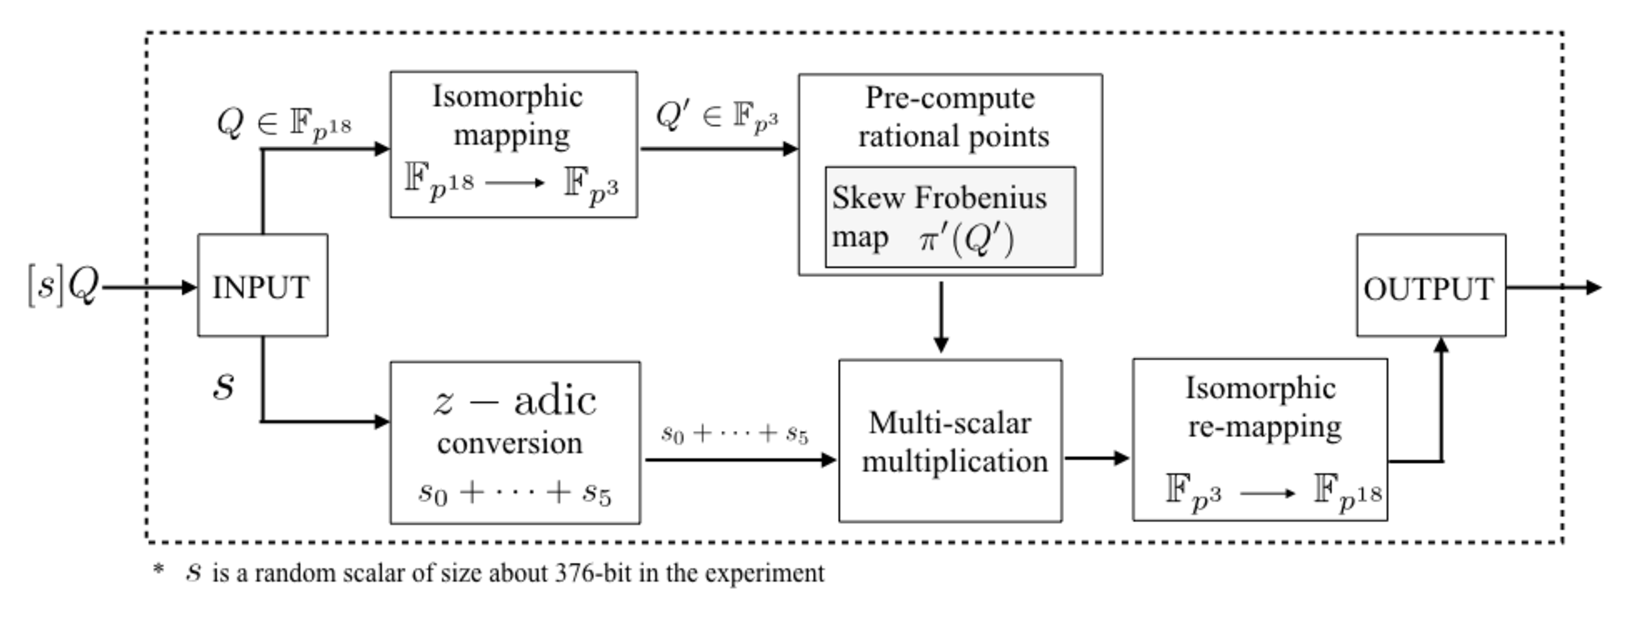
\includegraphics[width=\linewidth, keepaspectratio]{process.eps}
	%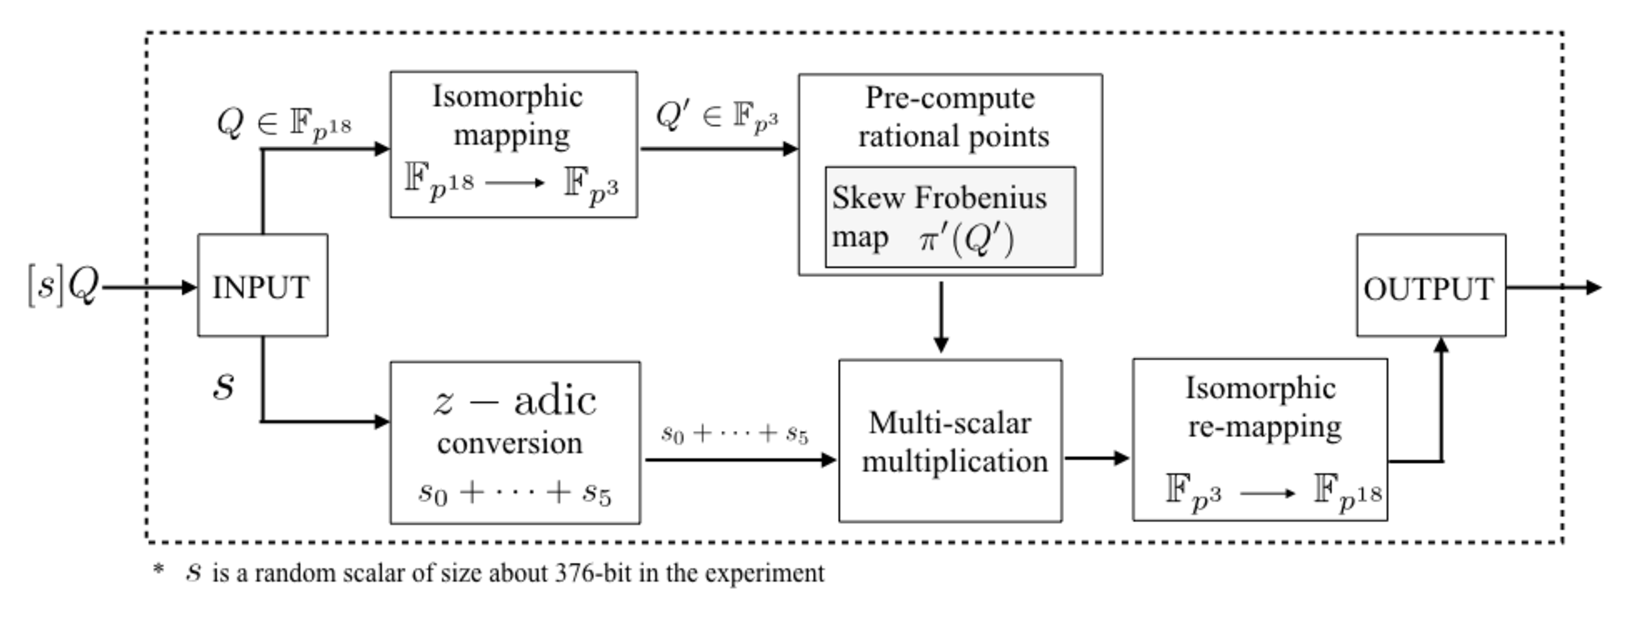
\includegraphics[width=6.5in]{process.eps}
	\caption{Overview of the proposed scalar multiplication for KSS-18 curve.}
	\label{fig:_overallprocess_towering_chapter_g2scm_kss18}
\end{figure*}
Rational point groups $\g1$, $\g2$ and multiplicative group $\g3$ groups will be defined at the beginning. Then a rational point $Q\in \g2 \subset E(\F{p}{18})$ will be calculated.
$Q$ has a  special vector representation with 18 $\Fp$ elements for each coordinates. 
A random scalar $s$ will be considered for scalar multiplication of $[s]Q$ which is denoted as input in  Figure \ref{fig:_overallprocess_towering_chapter_g2scm_kss18}. After that we will consider an isomorphic map of rational point $Q\in \g2 \subset E(\F{p}{18})$ to its sextic twisted rational point $Q' \in \g2' \subset E'(\F{p}{3})$. At the same time, we will obtain the $z$-adic representation of the scalar $s$. Next, some rational points defined over $E'(\FQTH)$ will be pre-computed by applying the skew Frobenius mapping. After that, a multi-scalar multiplication technique will be applied to calculate the scalar multiplication in parallel. The result of this scalar multiplication will be defined over $\FQTH$. Finally, the result of the multi-scalar multiplication will be re-mapped to a rational point in $E(\FQEN)$ to get the final result.

\subsection{\g1, \g2 and \g3 Groups} 
In the context of pairing-based cryptography, especially on KSS-18 curve, three groups $\g1, \g2$, and $\mathbb{G}_3$ are considered. From \cite{PAIRING:MANS13}, we define $\g1$, $\g2$ and $\g3$ as follows:
\begin{eqnarray}\label{eq:g1_chapter_g2scm_kss18}
\g1 & = &  E(\F{p}{18}) [r] \cap \text{Ker}(\pi_p - [1]), \nonumber \\
\g2 & = &  E(\F{p}{18}) [r] \cap \text{Ker}(\pi_p - [p]), \nonumber \\
\g3 & = & \mF{p}{18}/(\mF{p}{18})^r, \nonumber
\end{eqnarray}
\begin{equation}
\alpha : \g1 \times \g2 \rightarrow \g3,
\end{equation}
where $\alpha$ denotes Ate pairing. In the case of KSS-18 curve, $\g1, \g2$ are rational point groups and $\mathbb{G}_3$ is the multiplicative group in $\FQEN$. They have the same order $r$. 

In context of KSS-18 curve, let us consider a rational point $Q\in \g2 \subset E(\F{p}{18})$ where $Q$ satisfies the following relations,
\begin{eqnarray}\label{eq:Q_rel1_chapter_g2scm_kss18}
\big[p+1-t\big]Q & = & \cal O, \nonumber \\
\big[t-1\big]Q  & = & \big[p\big]Q.
\end{eqnarray}
\begin{eqnarray}\label{eq:Q_rel2_chapter_g2scm_kss18}
[\pi_p -p]Q & = &\cal O, \nonumber \\
\pi_p(Q) & = & [p]Q.
\end{eqnarray}
where  $[t-1]Q = \pi_p(Q)$, by substituting $[p]Q$ in \eqref{eq:Q_rel1_chapter_g2scm_kss18}.


\subsection{Isomorphic Mapping between \texorpdfstring{$Q$}{Q} and  \texorpdfstring{$Q'$}{Q'}}
\label{sec:ch:ieice2016:mappingQtoQprime}
Let us consider $E$ is the KSS-18 curve in base field $\FQTH$  and $E'$ is sextic twist of $E$ given as follows: 
\begin{eqnarray}
E:y^2 & = &x^3+b,\\
E':y^2 & = & x^3+bi, \label{eq:KSS18_Twist_chapter_g2scm_kss18}
\end{eqnarray}
where $b \in \Fp$; $x, y, i \in \FQTH$ and basis element $i$ is the quadratic and cubic non residue in $\FQTH$.

Rational point $Q\in \g2 \subset E(\F{p}{18})$ has a  special vector representation with 18 $\Fp$ elements for each $x_Q$ and $y_Q$ coordinates.
Figure \ref{fig:Q_structure_chapter_g2scm_kss18} shows the structure of the coefficients of $Q \in \FQEN$ and its sextic twisted isomorphic rational point $Q' \in \FQTH$ in KSS-18 curve.
\begin{figure}[ht]
	\centering
	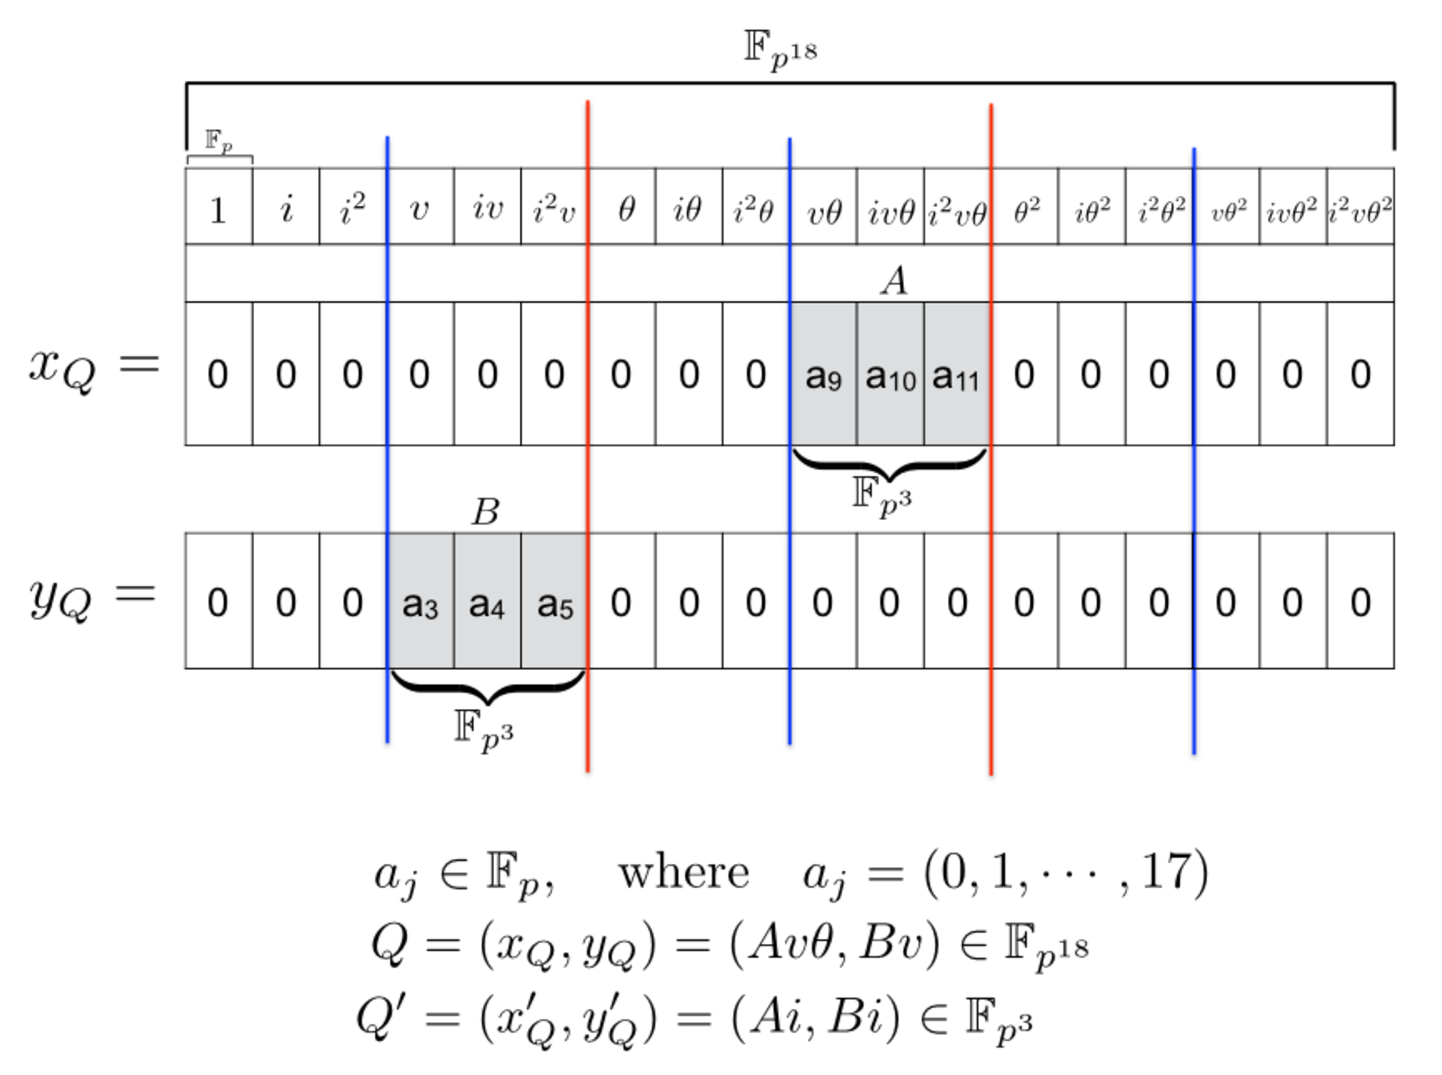
\includegraphics[width=\linewidth, keepaspectratio]{structure.eps}
	\caption{ $Q \in \FQEN$ and its sextic twisted isomorphic rational point $Q' \in \FQTH$ structure in KSS-18 curve.}
	\label{fig:Q_structure_chapter_g2scm_kss18}
\end{figure}
Among 18 elements, there are 3 continuous nonzero $\Fp$ elements which belongs to a $\FQTH$ element. The other coefficients are zero.
In this chapter, considering parameter settings given in Table \ref{table:parameters_chapter_g2scm_kss18} of section 4; $Q$ is given as $Q = (Av\theta, Bv)$,  showed in Figure \ref{fig:Q_structure_chapter_g2scm_kss18}, where $A, B \in \FQTH$ and $v$ and $\theta$ are the basis elements of $\F{p}{6}$ and $\FQEN$ respectively. 

Let us consider the sextic twisted isomorphic subfield rational point of $Q$ as $Q' \in \g2' \subset E'(\F{p}{3})$ and $x'$ and $y'$ as the coordinates of $Q'$.

\subsubsection{Mapping \texorpdfstring{$Q = (Av\theta, Bv)$}{}  to the Rational Point  \texorpdfstring{$Q' = (x',y')$}{}}

Let's multiply  $\theta^{-6}$ with both side of \eqref{eq:KSS18_Twist_chapter_g2scm_kss18}, where $i=\theta^6$ and $v = \theta^3$.
\begin{equation}\label{eq:sextic_div_theta_chapter_g2scm_kss18}
E':  \Big(\frac{y}{\theta^3}\Big)^2  = \Big(\frac{x}{\theta^2}\Big)^3+ b.
\end{equation}
Now $\theta^{-2}$ and $\theta^{-3}$ of  \eqref{eq:sextic_div_theta_chapter_g2scm_kss18} can be represented as follows:
\begin{subequations}
	\begin{eqnarray}
	\theta^{-2} &  = & i^{-1}\theta^{4}, \label{eq:thta2_4_chapter_g2scm_kss18} \\
	\theta^{-3} &  = & i^{-1}\theta^{3}.\label{eq:thta_3_chapter_g2scm_kss18} 
	\end{eqnarray}
\end{subequations}
Let us represent $Q = (Av\theta, Bv)$  as follows:
\begin{equation}\label{eq:mapefp18_toefp3_chapter_g2scm_kss18}
Q  =  (A\theta^4, B\theta^3), \quad \text{where $v=\theta^3$}.
\end{equation}
From \eqref{eq:thta2_4_chapter_g2scm_kss18} and \eqref{eq:thta_3_chapter_g2scm_kss18} $ \theta^4 = i\theta^{-2}$ and $\theta^3 = i\theta^{-3}$  is substituted in \eqref{eq:mapefp18_toefp3_chapter_g2scm_kss18}  as 
follows:
\begin{equation}\label{eq:mapefp18_toefp3_chapter_g2scm_kss18.1}
Q  =  (Ai\theta^{-2}, Bi\theta^{-3}),
\end{equation}
where $Ai = x'$ and $Bi = y'$ are the coordinates of $Q' =(x',y') \in \FQTH$. 
From the structure of $\FQEN$, given in \ref{eq:KSS18_towering_chapter_g2scm_kss18}, this mapping has required no expensive arithmetic operation. Multiplication by the basis element $i$ in $\FQTH$ can be done by 1 bit wise left shifting since $c=2$ is considered for towering in \ref{eq:KSS18_towering_chapter_g2scm_kss18}.


\subsection{\texorpdfstring{$z$}{}-adic Representation of Scalar \texorpdfstring{$s$}{}}\index{$z$-adic decomposition}
\label{section_zadic_chapter_g2scm_kss18}
In context of KSS-18 curve, properties of $Q$ will be obtained to define the \eqref{eq:Q_rel2_chapter_g2scm_kss18} relation.
Next, a random scalar $s$ will be considered for scalar multiplication of $[s]Q$. Then $(t-1)$-adic representation of $s$ will be considered as Figure \ref{fig:t_adic_chapter_g2scm_kss18}. Here $s$ will be divided into two smaller coefficients $S_H$, $S_L$ where  $S_L$ denotes lower bits of $s$,  will be nearly equal to the size of $(t-1)$. On the other hand the higher order bits $S_H$ will be the half of the size of $(t-1)$. Next, $z$-adic representation of $S_H$ and $S_L$ will be considered. Figure \ref{fig:z_adicl_chapter_g2scm_kss18}, shows the $z$-adic representation from where we find that scalar $s$ is divided into 6 coefficients of $z$, where the size of $z$ is about $1/4$ of that of $(t-1)$ according to \eqref{eq:kss_trace_chapter_g2scm_kss18}. 

Figure \ref{fig:t_adic_chapter_g2scm_kss18} shows $(t-1)$-adic representation of scalar $s$. 
\begin{figure}[ht]
	\centering
	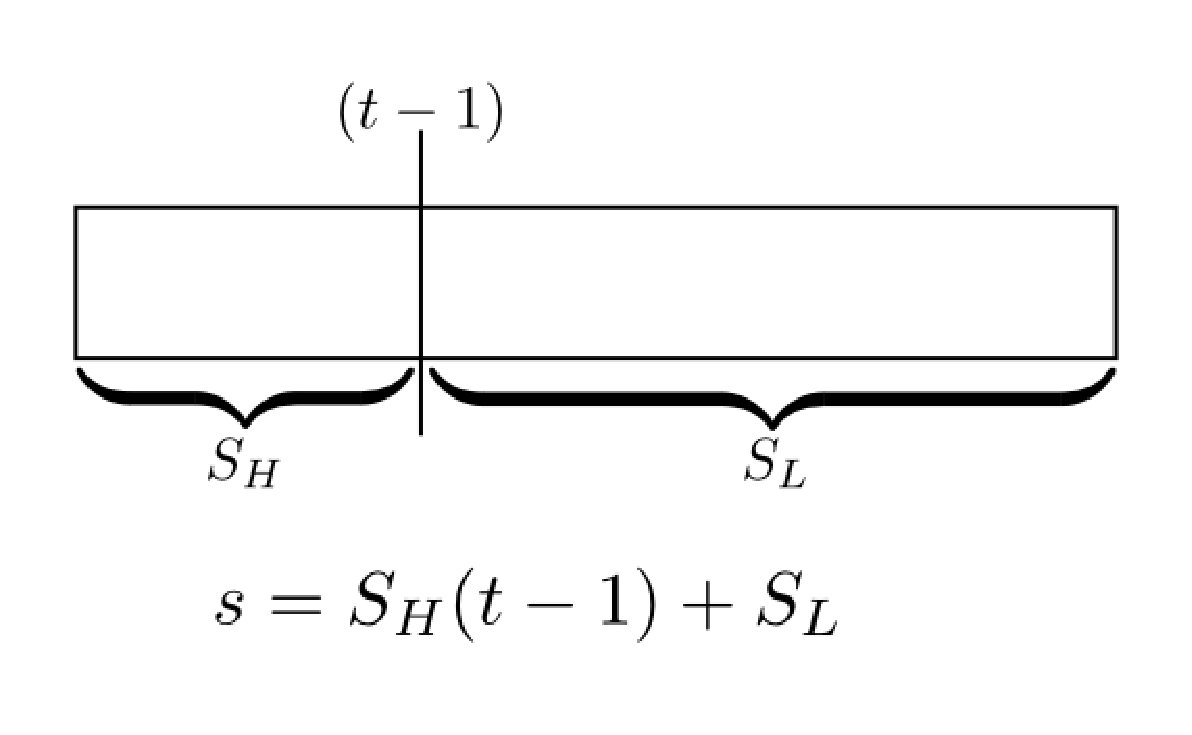
\includegraphics[width=0.7\linewidth, height=\textheight, keepaspectratio]{t_adic.eps}
	%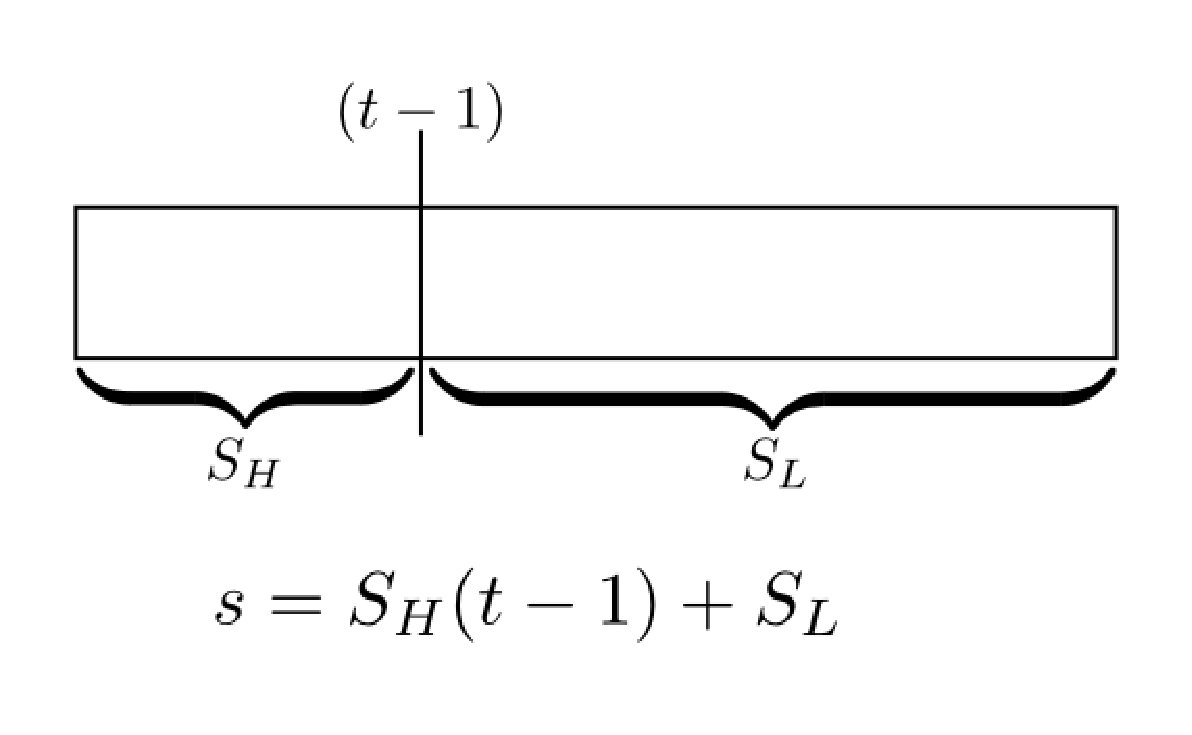
\includegraphics[width=0.7\columnwidth]{t_adic.eps}
	\caption{$(t-1)$ -adic representation of scalar $s$.}
	\label{fig:t_adic_chapter_g2scm_kss18}
\end{figure}

\begin{figure}[ht]
	\centering
	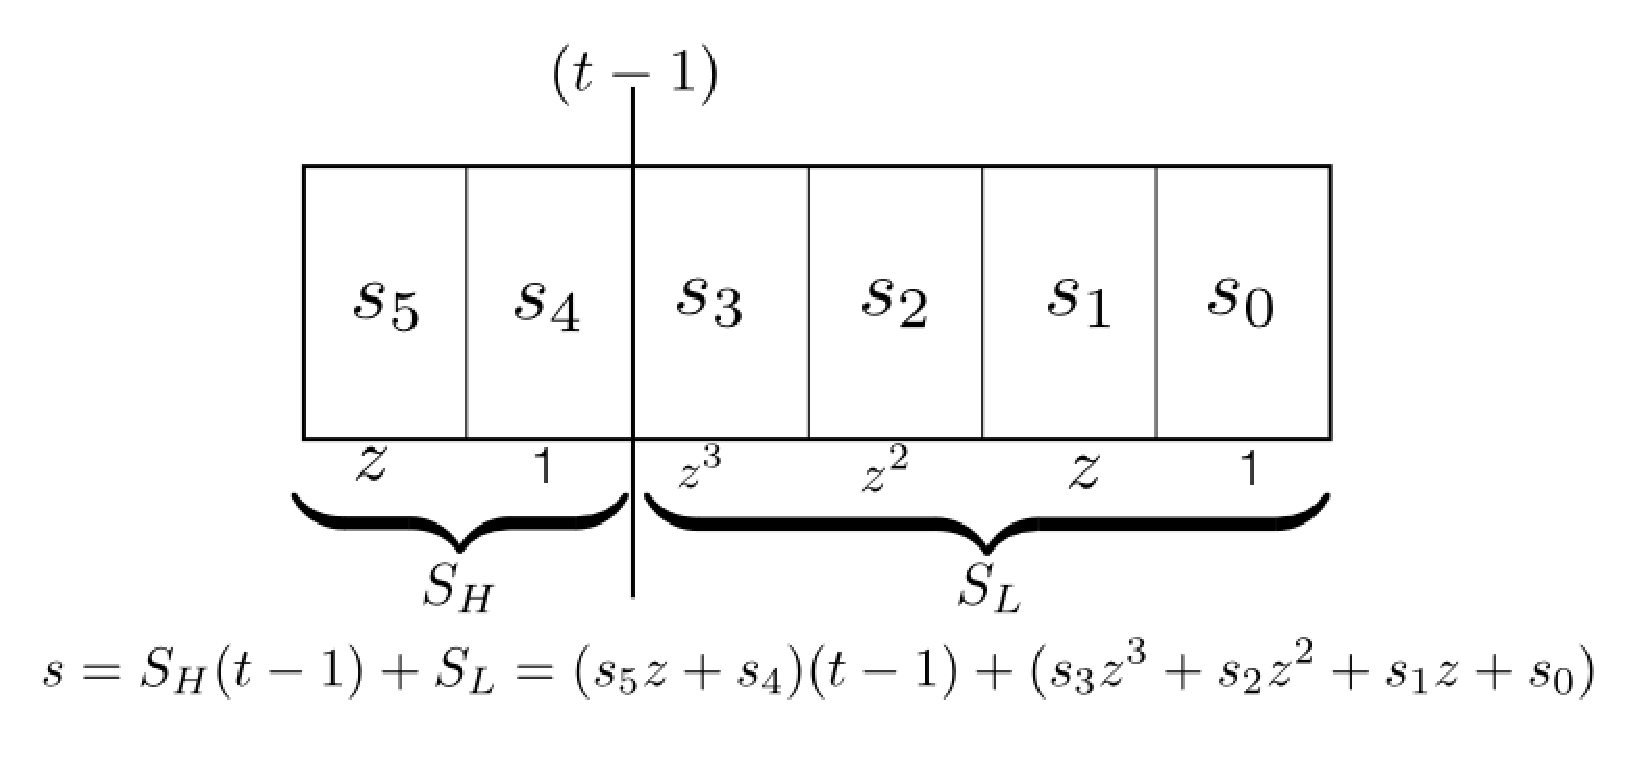
\includegraphics[width=\linewidth, height=\textheight, keepaspectratio]{z_adic.eps}
	\caption{$z$-adic and $(t-1)$-adic representation of scalar $s$.}
	\label{fig:z_adicl_chapter_g2scm_kss18}
\end{figure}

Figure \ref{fig:z_adicl_chapter_g2scm_kss18} shows the  $z$-adic representation of scalar $s$. 
In the previous work on Optimal-Ate pairing, Aranha et al. \cite{PAIRING:AFKMR12} derived a relation from the parameter setting of KSS-18 curve as follows:
\begin{equation}\label{eq:aranha_relationkss18_chapter_g2scm_kss18}
z+3p-p^4 \equiv 0 \bmod {r},
\end{equation}
where $z$ is the \textit{mother parameter} of KSS-18 curve which is about six times smaller than order $r$. 

Since $Q$ is mapped to its ismorphic sextic twisted rational point $Q'$, therefore we can consider scalar multiplication $[s]Q'$ where $0 \leq s < r$. $[s]Q'$ will be calculated in $\FQTH$ and eventually the result will be mapped to $\FQEN$ to get the final result. From \eqref{eq:kss_degree_chapter_g2scm_kss18} we know $r$ is the order of KSS-18 curve  where $[r]Q=\cal O$. Here, the bit size of $s$ is nearly equal to $r$. In KSS-18 curve $t$ is  $4/6$ times of  $r$. Therefore, let us first consider $(t-1)$-adic representation of $s$ as follows:
\begin{equation}\label{eq:t-1_adic_chapter_g2scm_kss18}
s =  S_H(t-1)+S_L,
\end{equation}
where $s$ will be separated into two coefficients $S_H$ and $S_L$. $S_L$ will be nearly equal to the size of $(t-1)$ and $S_H$ will be about half of $(t-1)$. 
In what follows, $z$-adic representation of $S_H$ and $S_L$ is given as:
\begin{eqnarray}\label{eq:eqn_scalar_mul_chapter_g2scm_kss18_Q}
S_H & =  & s_5+ s_4,\nonumber \\
S_L & = & s_3 z^3+s_2 z^2+s_1 z+s_0.\nonumber 
\end{eqnarray}
Finally $s$ can be represented as 6 coefficients as follows:
\begin{eqnarray}\label{eq:sclar_final_rep_chapter_g2scm_kss18}
s & =  & \sum_{i=0}^{3} s_iz^i + (s_4+s_5z)(t-1),\nonumber \\
s & = & (s_0+s_1z) + (s_2 +s_3z)z^2 +(s_4+s_5z)(t-1).
\end{eqnarray}

\subsection{Reducing Elliptic Curve Doubling in \texorpdfstring{$[s]Q'$}{[s]Q}}
Let us consider a scalar multiplication of $Q' \in \g2'$ in \eqref{eq:sclar_final_rep_chapter_g2scm_kss18} as follows:
\begin{equation}\label{eq:proposed_scm_1_chapter_g2scm_kss18}
[s]Q' =  (s_0+s_1z)Q' + (s_2 +s_3z)z^2Q'  +(s_4+s_5z)(t-1)Q'.
\end{equation}
In what follows, $z^2Q'$, $(t-1)Q'$ of \eqref{eq:proposed_scm_1_chapter_g2scm_kss18} is denoted as $Q_1'$ and $Q_2'$ respectively. From \eqref{eq:aranha_relationkss18_chapter_g2scm_kss18} and \eqref{eq:Q_rel2_chapter_g2scm_kss18} we can derive the $Q_1'$ as follows:
\begin{eqnarray}\label{eq:Q1_chapter_g2scm_kss18}
Q_1'& = & z^2 Q', \nonumber \\
& = & (9p^2-6p^5+p^8)Q',\nonumber \\
& = & 9\pi'^2(Q')-6\pi'^5(Q')+\pi'^8(Q').
\end{eqnarray}
where $\pi' (Q')$ is called the \textbf{skew Frobenius mapping} of rational point $Q' \in E'(\FQTH)$.
\eqref{eq:Q1_chapter_g2scm_kss18} is simplified as follows by utilizing the properties of cyclotomic polynomial.
\begin{eqnarray}\label{eq:Q11_chapter_g2scm_kss18}
Q_1' & = & 8\pi'^2(Q')-5\pi'^5(Q'),  \nonumber\\
& = & \pi'^2(8Q')-\pi'^5(5Q'). 
\end{eqnarray}
And from the \eqref{eq:Q_rel1_chapter_g2scm_kss18} and \eqref{eq:Q_rel2_chapter_g2scm_kss18}, $Q_2'$ is derived as,
\begin{equation}\label{eq:proposed_scm_2_chapter_g2scm_kss18}
Q_2' = \pi' (Q').
\end{equation}
Substituting \eqref{eq:Q11_chapter_g2scm_kss18} and \eqref{eq:proposed_scm_2_chapter_g2scm_kss18} in \eqref{eq:proposed_scm_1_chapter_g2scm_kss18}, the following relation is obtained. 
\begin{equation}\label{eq:proposed_scm_0_chapter_g2scm_kss18}
s[Q'] =  (s_0+s_1z)Q' + (s_2 +s_3z)Q_1' +(s_4+s_5z)Q_2'.
\end{equation}
Using $z \equiv -3p + p^4$ (mod $r$) from \eqref{eq:aranha_relationkss18_chapter_g2scm_kss18}, $z(Q')$ can be pre-computed as follows:
\begin{equation}
z(Q') = \pi'(-3Q') +\pi'^4(Q').
\end{equation}

Table \ref{table:pre-compute_chapter_g2scm_kss18} shows all the pre-computed values of rational points defined over $\FQTH$ for the proposed method. 
Pre-computed rational points are denoted inside angular bracket such as $<Q'+Q_2'>$ in this chapter. 

\renewcommand{\baselinestretch}{1.5}
\begin{table}[!ht]
	\centering
	\caption{13 pre-computed values of rational points.}
	\label{table:pre-compute_chapter_g2scm_kss18}
	\begin{tabular}{|c|c|}
		\hline 
		Pre-computed rational points & Skew Frobenius mapped rational points\\ 
		\hline 
		& $z(Q')$ \\ 
		\hline 
		$Q_1'$ & $z(Q_1')$  \\ 
		\hline 
		$Q_2'$ & $z(Q_2')$ \\ 
		\hline 
		$Q_1'+Q_2'$ & \quad  $ z(Q_1')+ z(Q_2') $ \quad \\ 
		\hline 
		$Q'+Q_2'$ & $ z(Q')+ z(Q_2') $ \\ 
		\hline 
		$Q'+Q_1'$ & $  z(Q')+ z(Q_1') $ \\ 
		\hline 
		\quad $Q'+Q_1'+Q_2'$ \quad  \quad &   \quad  $ z(Q')+ z(Q_1')+ z(Q_2')$  \quad \\ 
		\hline 
	\end{tabular} 
\end{table}
\renewcommand{\baselinestretch}{1.0}

\subsection{Skew Frobenius Map of \texorpdfstring{$\g{2}$}{} Points in KSS-18 Curve}
\index{KSS-18: Skew Frobenius map}
Similar to Frobenius mapping, skew Frobenius map is the $p$-th power over the sextic twisted isomorphic rational points such as  $Q' = (x',y')$ as 
follows:
\begin{equation}
\pi' : (x',y') \mapsto  (x'^p,y'^p)
\end{equation}
The detailed procedure to obtain the skew Frobenius map of $Q' = (x',y') \in \g2' \subset E'(\FQTH)$ is given bellow:
\begin{subequations}
	\begin{eqnarray}\label{eq:skew_x_prime_chapter_g2scm_kss18}
	\pi'(x') & = & (x')^p(i)^{1-p}(v)^{p-1}(\theta)^{p-1} \nonumber \\
	& = & (x')^p(i)^{1-p}(\theta^4)^{p-1} \nonumber \\
	& = & (x')^p (i^{-1})^pi(\theta^{p-1})^4 \nonumber \\
	& = & (x')^p (i^{-1})^pi(i^{\frac{p-1}{6}})^4  \mbox{\quad where $\theta^6=i$} \nonumber \\
	& = & (x')^p (i^{-1})^pi(i^{\frac{p-1}{6} -1}i)^4  \nonumber \\
	& = & (x')^p (i^{-1})^pi(i^{3\frac{\frac{p-7}{6}}{3}})^4i^4  \nonumber \\
	& = & (x')^p (i^{-1})^pi(2^{\frac{p-7}{18}})^42i  \mbox{\quad where $i^3=2$} \nonumber \\
	& = & (x')^p (i^{-1})^pi(2^{\frac{2p-14}{9}+1})i  \nonumber \\
	& = & (x')^p (i^{-1})^pi(2^{\frac{2p-5}{9}})i,
	\end{eqnarray}
	\begin{eqnarray}\label{eq:skew_y_prime_chapter_g2scm_kss18}
	\pi'(y') & = & (y')^p(i)^{1-p}(v)^{p-1} \nonumber \\
	& = & (y')^p (i^{-1})^pi(v^{6\frac{p-1}{6}})  \nonumber \\
	& = & (y')^p (i^{-1})^pi(i^{3\frac{p-1}{6}})  \nonumber \\
	& = & (y')^p (i^{-1})^pi2^{\frac{p-1}{6}}.
	\end{eqnarray}
\end{subequations}
Here $(i^{-1})^pi$, $(2^{\frac{2p-5}{9}})i$  and $2^{\frac{p-1}{6}}$ can be pre-computed. 

\subsection{Multi-Scalar Multiplication}
Applying the the multi-scalar multiplication technique in \eqref{eq:proposed_scm_0_chapter_g2scm_kss18} we can efficiently calculate the scalar multiplication in $\FQTH$. Figure \ref{eq:fig:z_sml_chapter_g2scm_kss18} shows an example of this multiplication.
Suppose in an arbitrary index, from left to right, bit pattern of $s_1$, $s_3$, $s_5$ is 101 and at the same index $s_0$, $s_2$, $s_4$ is 111.
Therefore we apply the pre-computed points $< z(Q')+z(Q_2') >$ and $<Q'+Q_1'+Q_2'>$ as ECA in parallel.
Then we perform ECD and move to the right next bit index to repeat the process until maximum length $z$-adic coefficient becomes zero.
\begin{figure}[!ht]
	\centering
	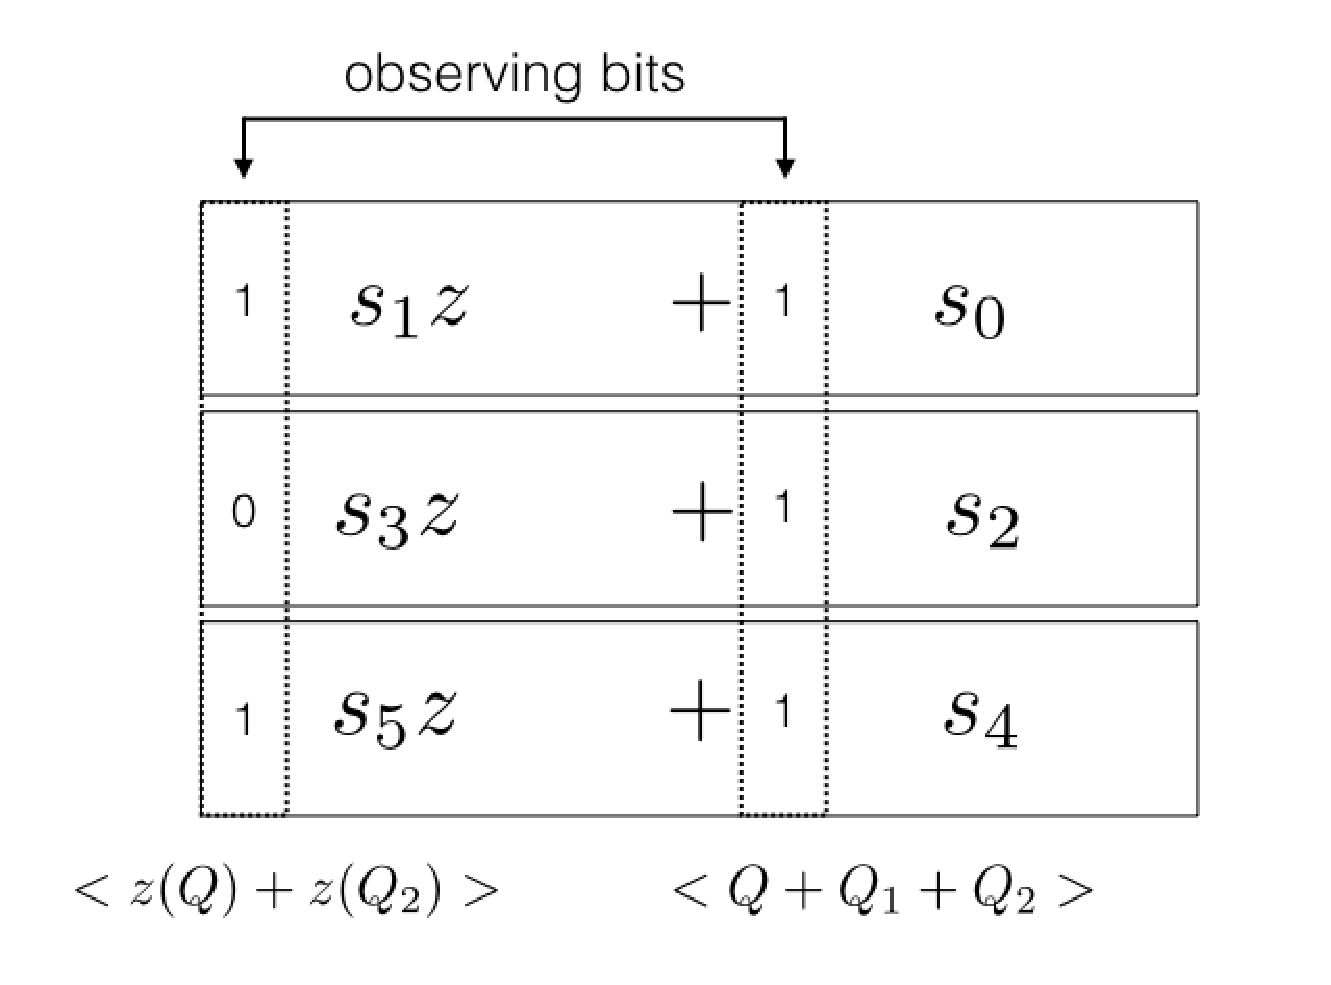
\includegraphics[width=0.8\linewidth, height=\textheight, keepaspectratio]{z_sm.eps}
	\caption{Multi-scalar multiplication of $s$ with Frobenius mapping.}
	\label{eq:fig:z_sml_chapter_g2scm_kss18}
\end{figure}

As shown in Figure \ref{eq:fig:z_sml_chapter_g2scm_kss18}, during scalar multiplication, we are considering 3 pair of coefficients of $z$-adic representation as shown in  \eqref{eq:sclar_final_rep_chapter_g2scm_kss18}. If we consider 6-coefficients for parallelization, it will require $2^6 \times 2$ pre-computed points. The chance of appearing each pre-computed point in the calculation will be once that causes redundancy.  

\subsubsection{Re-mapping Rational Points from \texorpdfstring{$E'(\FQTH)$}{} to  \texorpdfstring{$E(\FQEN)$}{}}
After the multi-scalar multiplication, we need to remap the result to $\FQEN$. For example let us consider re-mapping of $Q' =(x',y') \in E'(\FQTH)$ to $Q =(Av\theta,Bv) \in E(\FQEN)$. From \eqref{eq:thta2_4_chapter_g2scm_kss18}, \eqref{eq:thta_3_chapter_g2scm_kss18} and \eqref{eq:sextic_div_theta_chapter_g2scm_kss18} it can be obtained as follows:
\begin{subequations}
	\begin{eqnarray}
	x i^{-1}\theta^{4} & = & Av\theta, \nonumber \\
	y i^{-1}\theta^{3} & = & Bv, \nonumber
	\end{eqnarray}
\end{subequations}
which resembles that $Q= (Av\theta, Bv)$. Therefore it means that multiplying $i^{-1}$ with the $Q'$ coordinates and placing the resulted coefficients in the corresponding position of the coefficients in $Q$, will map $Q'$ to $Q$.
This mapping costs one $\FQTH$ inversion of $i$ which can be pre-computed and one $\Fp$ multiplication.

\section{Simulation Result}
This section shows the experimental result with the calculation cost.
In the experiment, we have compared the proposed method with three well-studied methods of scalar multiplication named binary method, sliding-window method, and non-adjacent form (NAF) method. 
The mother parameter $z$ is  selected according to the suggestion of Scott et al. \cite{IMA:Scott11} to obtain $p = 508 \approx 511$-bit and $r =  376 \approx 384$-bit  to simulate in 192-bit security level.
Table \ref{table:parameters_chapter_g2scm_kss18} shows the parameter settings considered for the simulation.

\renewcommand{\baselinestretch}{1.5}
\begin{table}[htb]
	\begin{center}
		\caption{Parameter settings used in the experiment.}
		%\resizebox{0.7\columnwidth}{!}{
		\begin{tabular}{|c|c|}
			\hline
			Defined KSS-18 curve & $y^2 = x^3 + 11$ \\ \hline
			Mother parameter $z$ & 65-bit \\ \hline
			Characteristics  $p(z)$ & 511-bit \\ \hline
			Order  $r(z)$ & 376-bit \\ \hline
			Frobenius trace $t(z)$ & 255-bit \\ \hline
			Persuadable security level & 192-bit \\ \hline
		\end{tabular}
		%}
		\label{table:parameters_chapter_g2scm_kss18}
	\end{center}
\end{table}
\renewcommand{\baselinestretch}{1.0}

Table \ref{table:comEnvironment_chapter_g2scm_kss18} shows the environment, used to experiment and evaluate the proposed method.  
\renewcommand{\baselinestretch}{1.5}
\begin{table}[!ht]
	\renewcommand{\arraystretch}{1.3}
	\centering
	\caption{ Computational environment.}
	\label{table:comEnvironment_chapter_g2scm_kss18}
	\resizebox{\columnwidth}{!}{
		\begin{tabular}{|c|c|c|}
			\hline 
			& PC & iPhone6s \\ 
			\hline \hline 
			CPU {\textsuperscript{*}} & \quad 2.7 GHz Intel Core i5 \quad & \quad Apple A9 Dual-core 1.84 GHz \quad \\ 
			\hline 
			Memory & 16 GB & 2 GB \\ 
			\hline 
			OS & Mac OS X 10.11.6 &  iOS 10.0 \\ 
			\hline 
			Compiler & gcc 4.2.1 & gcc 4.2.1 \\ 
			\hline 
			\quad Programming Language \quad  & C & Objective-C, C \\ 
			\hline 
			Library &  GMP 6.1.0 & GMP 6.1.0\\ 
			\hline 
			\multicolumn{3}{l}{\textsuperscript{*}\footnotesize{Only single core is used from two cores.}}\\
		\end{tabular} 
	}
\end{table}
\renewcommand{\baselinestretch}{1.0}

In experiment 100 random scalar numbers of size less than order $r$ ( 378-bit) is generated.
13  ECA counted for pre-computed rational points is taken into account while the average is calculated for the proposed method.
A window size of 4-bit is considered for the sliding-window method. 
Therefore 14 pre-computed ECA is required. 
Besides, the average execution time of the proposed method and the three other methods are also compared along with the operation count.

In what follows, ``\textit{\textbf{With isomorphic mapping}}'' refers that skew Frobenius mapping technique is applied for Binary, Sliding-window, and NAF methods. Therefore the scalar multiplication is calculated in $\FQTH$ extension field.
Moreover, for the Proposed method, it is skew Frobenius mapping with multi-scalar multiplication. 
On the other hand ``\textit{\textbf{Without isomorphic mapping}}'' denotes that Frobenius map is not applied for any of the methods.
In this case, all the scalar multiplication is calculated in $\FQEN$ extension field.

%\medskip\noindent
\renewcommand{\baselinestretch}{1.5}
\begin{table}[ht]
	\centering
	\caption{Comparison of average number of ECA and ECD for $\g{2}$ SCM in KSS-18.}
	\label{table:operationcount_chapter_g2scm_kss18}
	%\resizebox{\columnwidth}{!}{
	\begin{tabular}{l|l|l|}
		\cline{2-3}
		& \multicolumn{2}{l|}{Count of average number of ECA, ECD} \\ \hline
		\multicolumn{1}{|l|}{Methods}        & ECA      \quad     \quad       \quad \quad     \quad       \quad       & ECD                        \\ \hline
		\multicolumn{1}{|l|}{Binary}         & 186                         & 375                        \\ \hline
		\multicolumn{1}{|l|}{Sliding-window} & 102                         & 376                        \\ \hline
		\multicolumn{1}{|l|}{NAF}            & 127                         & 377                        \\ \hline
		\multicolumn{1}{|l|}{Proposed}       & 123                         & 64                         \\ \hline
	\end{tabular}
	%}
\end{table}
\renewcommand{\baselinestretch}{1.0}
In Table \ref{table:operationcount_chapter_g2scm_kss18} the operations of the \textit{Proposed} method are counted in $\FQTH$. On the other hand for Binary, Sliding-window and NAF method, the operations are counted in $\FQEN$.  The table clearly shows that in the \textit{Proposed} method requires about 6 times less ECD than any other methods.
The number of ECA has also reduced in the \textit{Proposed} method by about 30\% than binary method and the almost the same number of ECA of NAF. 

\renewcommand{\baselinestretch}{1.5}
\begin{table}[!ht]
	\centering
	\caption{Comparison of execution time in [ms] for scalar multiplication in KSS-18 curve.}
	\label{table:tab_executiontime_chapter_g2scm_kss18}
	\resizebox{\columnwidth}{!}{
		\begin{tabular}{|c|c|c|c|c|}
			\cline{2-5}
			\multicolumn{1}{c|}{} & 
			\multicolumn{4}{c|}{Execution time in [ms] }\\
			\cline{2-5}
			\multicolumn{1}{c|}{} & 
			\multicolumn{2}{c|}{With isomorphic mapping}&
			\multicolumn{2}{c|}{Without isomorphic mapping }\\
			\hline
			Methods & 
			PC &  iPhone6s &
			PC &  iPhone6s \\
			\hline
			Binary  
			&  $5.4 \times 10^1$  &  $8.4 \times 10^1$ 
			&  $1.2 \times 10^3$  &  $1.8 \times 10^3$ \\
			\hline
			Sliding-window 
			&  $4.8 \times 10^1$  &  $7.5 \times 10^1$ 
			&  $1.0 \times 10^3$  &  $1.6 \times 10^3$ \\
			\hline
			NAF
			&  $5.3 \times 10^1$  &  $7.7 \times 10^1$ 
			&  $1.6 \times 10^3$  &  $1.7 \times 10^3$ \\
			\hline
			Proposed
			&  $1.6 \times 10^1$  &  $2.4 \times 10^1$ 
			&  -  &  - \\
			\hline
			Multi-scalar  (only)
			&  -  &  -
			&  $3.4 \times 10^2$  &  $5.5 \times 10^2$ \\
			\hline
		\end{tabular}
	}
\end{table}
\renewcommand{\baselinestretch}{1.0}

Analyzing  Table \ref{table:tab_executiontime_chapter_g2scm_kss18}, we can find that when isomorphic mapping and skew Frobenius mapping is not adapted for  Binary, Sliding-window, and NAF, then the scalar multiplication of proposed method is more than 60 times faster than other methods. However when the isomorphic mapping is applied for the other methods, then our proposed technique is more than 3 times faster. Another essential comparison shows that when only multi-scalar multiplication is applied, then our proposed methods is about 20 times faster. 
In every scenario, our proposed method is faster than the other commonly used approaches.


The main focus of this experiment is to evaluate the acceleration ratio of scalar multiplication by applying the proposed approach on $\g2$ rational point group of  KSS curve of embedding degree 18. The experiment does not focus on efficiently implementing scalar multiplication for a particular environment. 

\section{Summary}
In this chapter, we have proposed an efficient method to calculate elliptic curve scalar multiplication using skew Frobenius mapping over KSS-18 curve in the context of pairing-based cryptography. 
Utilizing the skew Frobenius map along with the multi-scalar multiplication procedure, an efficient scalar multiplication method for KSS-18 curve is proposed in the chapter.
In addition to the theoretic proposal, this chapter has also presented a comparative simulation of the proposed approach with the plain binary method, sliding window method and non-adjacent form (NAF) for scalar multiplication. 
%The simulation shows that the proposed method is about 60 times faster than the plain implementation of other compared methods.
We have also applied $(t-1)$-adic and $z$-adic representation on the scalar and have applied multi-scalar multiplication technique to calculate scalar multiplication in parallel. 
We have evaluated and analyzed the improvement by implementing an experiment for the large size integer in 192-bit security level. 
According to the simulation result multi-scalar multiplication after applying skew Frobenius mapping in $\g2'$ can accelerate the scalar multiplication in $\g2 \subset E(\FQEN)$ by more than 60 times than scalar multiplication of $\g2$ rational point directly in $\FQEN$. 
 

%%=============CANDAR 2016 IJNC/JICCE sparse is Chapter5====================
%\chapter{CANDAR 2016} 
%
        \title{Isomorphic Mapping for Ate-based Pairing over KSS Curve of Embedding Degree 18}

        
        

        Pairing based cryptography is considered as the next generation of security for which it attracts many researcher to work on faster and efficient pairing to make it practical. Among the several challenges of efficient pairing; efficient scalar multiplication of rational point defined over extension field of degree $k \geq 12$ is important. 
        %In Ate-based pairing, efficient arithmetic operation over the higher degree rational point groups reflects on the efficiency of the pairing calculation. Arithmetic over higher degree takes more time than arithmetic over lower degree groups. 
        However, there exists isomorphic rational point group defined over relatively lower degree extension field.
        %The important part of this process is mapping from higher degree group to lower degree isomorphic group and its reverse mapping. 
        Exploiting such property, this paper has showed a mapping technique between isomorphic rational point groups in the context of Ate-based pairing with Kachisa-Schaefer-Scott (KSS) pairing friendly curve of embedding degree $k = 18$. In the case of KSS curve, there exists sub-field sextic twisted curve that includes sextic twisted isomorphic rational point group defined over $\FQTH$. This paper has showed the mapping procedure from  certain $\FQEN$ rational point group to its sub-field isomorphic rational point group in $\FQTH$ and vice versa. This paper has also showed that scalar multiplication is about 20 times faster after applying the proposed mapping  which in-turns resembles that the impact of this mapping will greatly enhance the pairing operation in KSS curve.
        
        \section{Introduction}
         At the advent of this century, Sakai et al. \cite{sakai} and Joux et al. \cite{joux} independently proposed a cryptosystem based on elliptic curve pairing. Since then, pairing based cryptography has attracted many researchers and it has been considered as the basis of next generation security. Many researchers have proposed several innovative pairing based cryptographic applications such as ID-based encryption \cite{sakai}, broadcast encryption \cite{boradcast} and group signature authentication \cite{group_sign_1} that upsurge the popularity of pairing based cryptography.
        In such outcome, Ate-based pairings such as Ate \cite{ate}, R-ate \cite{r_ate}, Optimal-ate \cite{op_ate_p}, twisted Ate  \cite{twisted_ate} and $\chi$-Ate \cite{chibasedBN} pairings have gained much attention since they have achieved quite efficient pairing calculation. 
        There is no alternative of efficient and fast pairing calculation for deploying pairing-based cryptographic applications in practical case. 
        This paper focuses on a peripheral technique of Ate-based pairings with Kachisa-Schaefer-Scott (KSS) curve \cite{kss}. 
        
        In general, pairing is a bilinear map from two rational point group $\g1$ and $\g2$ to a multiplicative group $\g3$ \cite{Silverman}, typically denoted by $\g1 \times \g2 \rightarrow \g3$.
        In the context of Ate-based pairing, $\g1$, $\g2$ and $\g3$ are defined as follows:
        \begin{eqnarray}\label{eq:g_1}
        \g1 & = &  E(\F{p}{k}) [r] \cap \text{Ker}(\pi_p - [1]), \nonumber \\
        \g2 & = &  E(\F{p}{k}) [r] \cap \text{Ker}(\pi_p - [p]), \nonumber \\
        \g3 & = & \mF{p}{k}/(\mF{p}{k})^r, \nonumber
        \end{eqnarray}
        \begin{equation}
        \alpha : \g1 \times \g2 \rightarrow \g3,  \nonumber
        \end{equation}
        where $\alpha$ denotes Ate pairing. Pairings are often found in certain extension field $\FQK$, where $p$ is the prime number, also know as characteristics  and the minimum extension degree $k$ is called \textit{embedding} degree. 
        The rational points $E(\FQK)$ are defined over a certain pairing friendly curve $E$ of embedded extension field of degree $k$.
        This paper has considered Kachisa-Schaefer-Scott (KSS) \cite{kss} pairing friendly curves of emebdding degree $k=18$ described in \cite{taxonomy}. 
        
        %Pairing on KSS curve satisfies 192-bit security level which is considered to be the basis of next generation security. 
        In Ate-based pairing with KSS curve, where $k = 18$,  pairing computations are done in higher degree extension field $\FQEN$. However, KSS curves defined over $\FQEN$ have the sextic twisted isomorphism over $\FQTH$. Therefore we can execute computations in the sub-field $\FQTH$. Exploiting such a property, different arithmetic operation of Ate-based pairing can be efficiently performed in $\g2$. In this paper we have mainly focused on mapping $\g2$ rational point from extension field $\FQEN$ to its sextic twisted sub-field $\FQTH$ and its reverse procedure. 
        
        The advantage of such mapping is examined by performing scalar multiplication on $\g2 \subset E(\FQEN)$ rational point, since scalar multiplication is required repeatedly in cryptographic calculation. 
        We have considered sub-field sextic twisted curve of KSS curve, denoted as $E'$. It includes sextic twisted isomorphic rational point group denoted as $\g2' \subset E(\FQTH)$. In KSS curve, $\g2$ is defined over $\FQEN$ whereas its sub-field isomorphic group $\g2'$ is defined over $\FQTH$. Then the proposed mapping technique is applied to map rational points of $\g2$ to its isomorphic $\g2'$. After that the scalar multiplication in $\g2'$ performed and the resulted points are re-mapped to $\g2$ in $\FQEN$.
        The experiment result shows  that efficiency of binary scalar multiplication is increased by more than 20 times in sub-field sextic twisted curve than scalar multiplication in $\FQEN$ without applying proposed mapping. The mapping and remapping requires one bit wise shifting in $\Fp$, one $\FQTH$ inversion which can be pre-computed and one $\Fp$ multiplication; hence the mapping procedure has no expensive arithmetic operation.
        
        The rest of the paper is organized as follows. 
        The fundamentals of elliptic curve arithmetic, scalar multiplication along with KSS curve over $\FQEN$ extension field and \textit{sextic twist} of KSS curve are described in section \Romannum{2}.
        In section \Romannum{3}, this paper describes the isomorphic mapping between the rational point $Q$ and $Q'$ in details. The experimental result is presented in section \Romannum{4} which shows that our scalar multiplication on $\g2$ point can be accelerated by 20 times by applying the proposed mapping technique in KSS curve. Finally section \Romannum{5} draws the conclusion with some outline how this work can be enhanced more as a future work.
        
        \section{Preliminaries}
        In this section this paper briefly overviews the fundamentals of elliptic curve operations. Elliptic curve scalar multiplication is reviewed briefly. Pairing friendly curve of embedded degree $k=18$, i.e., KSS curve and its properties are introduced in combination  with its construction procedure by towering.
        % Rational point groups for Ate-based pairing is introduced briefly. 
        \subsection{Elliptic curve}
        Let $\Fp$ be a prime field and $\Fq$ be its extension field. An elliptic curve \cite{ecc_book} defined over $\Fp$ is generally represented by \textit{affine coordinates} \cite{Silverman} as follows;
        \begin{equation}\label{ec_curve}
        E/\Fp : y^2=x^3+ax+b,
        \end{equation}
        where $ 4a^3+27b^2 \neq 0$ and $a,b \in \Fp$. A pair of coordinates $x$ and $y$ that satisfy \eqref{ec_curve} are known as \textit{rational points} on the curve. 
        
        $E(\F{q}{k})$ denotes an elliptic curve group where the definition field is $\F{q}{k}$ and $\#E(\F{q}{k})$ denotes its order. When the definition field is prime field $\Fp$ then $\#E(\Fp)$ can be represented as,
        \begin{equation}\label{order}
        \#E(\Fp) = p+1-t,
        \end{equation} 
        where $t$ is called the Frobenius trace of $E(\Fp)$.
        
        Let $E(\f{p})$ be the set of all rational points on the curve defined over $\Fp$ and it includes the point at infinity denoted by $\mathcal{O}$. 
        The order of $\EFP$ is denoted by $\SEFP$ where $\EFP$ forms an additive group for the elliptic addition. The set of rational points over $\Fq$, including $\mathcal{O}$ satisfying \eqref{ec_curve} is denoted by $E(\Fq)$. The order of $E(\Fq)$ is denoted by $\#E(\Fq)$.
        
        Let us consider two rational points using affine coordinates as $P_1= (x_1, y_1)$, $P_2 = (x_2, y_2)$, and their addition $R = P_1 + P_2$, where $\textit{R} = (x_3, y_3)$ and $P_1, P_2, R \in E(\Fq)$. Then the $x$ and $y$ coordinates of $R$ are calculated as follows:
        
        \begin{subequations}
        \begin{eqnarray}\label{eq:point_add}
        x_3 & = & \lambda^2-x_1-x_2 ,\\
         y_3 & = &(x_1-x_3)\lambda - y_1, 
        \end{eqnarray}
        where \mbox{$\lambda$} is given as follows:
        \begin{equation}\label{eq:point_solpe}
        \textstyle \lambda = 
        \begin{cases}
         \textstyle \frac{y_2 - y_1}{ x_2 -x_1}; \quad \mbox{$P_1 \neq P_2$},\\
         \textstyle \frac{3x_1^2+a}{2y_1}; \quad  \mbox{$P_1 = P_2$},\\
        \end{cases}
        \end{equation}
        \end{subequations}
        $\lambda$ is the tangent at the point on the curve and $\cal O$ is the additive unity in $E(\f{q})$. When $P_1 \neq P_2$ then $P_1+P_2$ is called elliptic curve addition (ECA). If $P_1=P_2$ then $P_1+P_2=2P_1$, which is known as elliptic curve doubling (ECD). 
        %\subsubsection{Scalar multiplication.}
        
        Let $[s]P_1$ be the scalar multiplication for the rational point $P_1$ with scalar $s$ as,
        
        \begin{equation}\label{scalar_mul}
        [s]P_1 = \sum_{i=0}^{s-1} P_1, \quad \text{$0 \leq s < r$},
        \end{equation}
        where $r$ is the order of the target rational point group. If $s = r$, where $r$ is the order of the curve then $[r]P_1 = \mathcal{O}$. When $[s]P_1 = P_2$, if $s$ is unknown, then the solving $s$ from $P_1$ and $P_2$ is known as elliptic curve discrete logarithm problem (ECDLP). The security of elliptic curve cryptography depends on the difficulty of solving ECDLP.
        
        The binary method is a widely recognized method for calculating the elliptic curve scalar multiplication. Algorithm \ref{alg:bin} shows the binary scalar multiplication algorithm. This algorithm scans the bits of scalar $s$ from  most significant bit to least significant bit. When $s[i] = 1$, it will perform ECA and ECD otherwise only ECD will be calculated. But this method is not resistant to side channel attack \cite{sca}.  
        
         \begin{algorithm}[H]
          \caption{Left-to-right binary algorithm for elliptic curve scalar multiplication}
          \label{alg:bin}
          \DontPrintSemicolon
          \hspace{-3ex}
          \KwIn{ $P$, $s$}\;
          \hspace{-3ex}
          \KwOut{$[s]P$} \;%output
          \nl $T$ $ \leftarrow$ $0$ \;
          \nl \For{$i = \lfloor \log_2 s \rfloor$ {\bf to} $0$} {\;
                  $T \leftarrow T  + T$\;
             \If{ $s[i] = 1$}{
                  $ T \leftarrow T + P$\;
                    } }\;
          \nl \text{return} $T$\;
          \end{algorithm}
        
        On the other hand Montgomery ladder algorithm is said to be resistant of side channel attack. Algorithm \ref{alg:mont} shows the Montgomery ladder algorithm for scalar multiplication. Montgomery ladder has some similarity with binary method except in each iteration it performs ECA and ECD. 
        
         \begin{algorithm}[H]
          \caption{Montgomery ladder algorithm for elliptic curve scalar multiplication}
          \label{alg:mont}
          \DontPrintSemicolon
          \hspace{-3ex}
          \KwIn{ $P$, $s$}\;
          \hspace{-3ex}
          \KwOut{$[s]P$} \;%output
          \nl $T_0$ $ \leftarrow$ $0$, $T_1$ $\leftarrow$ $P$ \;
          \nl \For{$i = \lfloor \log_2 s \rfloor$ {\bf to} $0$} {\;
         
             \If{ $s[i] =1$}{
                  $ T_0 \leftarrow T_0 + T_1$\;
                    $T_1 \leftarrow T_1 + T_1$\;
                    }
                    {\ElseIf{$s[i] = 0$}{ 
                    $T_1 \leftarrow T_0 + T_1$\;
                           $T_0 \leftarrow T_0 + T_0$\;}
                }
          }\;
          \nl \text{return} $T_0$\;
        \end{algorithm}
        This paper has considered left-to-right binary scalar multiplication for evaluating the efficiency of the proposed mapping operation. But from the view point of security binary method is vulnarable to side channel attack. Therefore this paper has also experimented with Montgomery ladder \cite{Silverman} for scalar multiplication evaluation.
        
        \subsection{KSS curve}
        Kachisa-Schaefer-Scott (KSS) curve \cite{kss} is a non super-singular pairing friendly elliptic curve of embedding degree 18, defined over $\FQEN$ as follows: 
        \begin{equation}\label{eq:KSS_curve}
        E/\FQEN:Y^2=X^3+b, \quad \mbox{$b \in \Fp$},
        \end{equation}
        where $b \neq 0$ and $X,Y \in \FQEN$. Its characteristic $p$, Frobenius trace $t$ and order $r$ are given systematically by using an integer variable $u$ as follows:
        \begin{subequations}
        \begin{eqnarray}
        p(u) &= & (u^8 +5u^7 +7u^6 +37u^5 +188u^4 +259u^3 \nonumber \\
        & & + 343u^2 +1763u+2401)/21,\\\label{eq:kss_char}
        r(u) &= &(u^6 + 37u^3 + 343)/343,\label{eq:kss_degree}  \\
        t(u) &=& (u^4 + 16u + 7)/7, \label{eq:kss_trace} 
        \end{eqnarray}
        \end{subequations} 
        
        where $u$ is such that $u \equiv 14$ (mod $42$) and the $\rho$ value is $\rho = (\log_2 p/\log_2 r) \approx 1.33$.
        
        %The order of rational points $\#E(\FQEN)$ on KSS curve can be obtained by the following relation.
        %\begin{equation}\label{eq:order_relation}
        %\#E(\FQEN) = p^{18}+1-t_{18},
        %\end{equation}
        %where $t_{18} = \alpha^{18}+\beta^{18}$ and $\alpha$, $\beta$ are complex numbers such that $\alpha+\beta = t$ and $\alpha\beta=p$.
        
        
        \subsection{$\FQEN$ extension field arithmetic}
        In pairing, arithmetic  operations are performed in higher degree extension fields, such as $\FQK$  for moderate value of $k$ \cite{Silverman}. Concequently, such higher extension field needs to be constructed as tower of extension fields \cite{const_ext} to perform arithmetic operation cost effectively.
        
        This paper has  represented extension field $\FQEN$ as a tower of sub-field to improve arithmetic operations. It has also used irreducible binomials introduced by Bailey et al. \cite{JC:BaiPaa01}. In what follows, this paper considers $3|(p-1)$ and $c$ is a quadratic and cubic non residue in $\Fp$. In context  of KSS-curve \cite{kss}, where $k=18$, $\FQEN$ is constructed as tower field with irreducible binomial as follows:
        \begin{equation}\label{eq:KSS_towering}
        \begin{cases}
        \F{p}{3} = \F{p}{}[i]/(i^3-c),  \\ 
        \F{p}{6} = \F{p}{3}[v]/(v^2-i),  \\ 
        \F{p}{18} = \F{p}{6}[\theta]/(\theta^3-v), \\ 
        \end{cases}
        \end{equation}
        where $c = 2$ is considered to be the best choice for efficient arithmetic.
        From the above towering construction we can find that $i=v^2=\theta^6$, where $i$ is the basis element of the base extension field $\FQTH$. 
        In the previous work of Aranha et al. \cite{PAIRING:AFKMR12}, explained the base extension field $\FQTH$ for the \textit{sextic twist} of KSS curve.
        
        \subsection{\g1, \g2 and \g3 groups.} In the context of pairing-based cryptography, especially on KSS curve, three groups $\g1, \g2$ and $\mathbb{G}_3$ are considered. From \cite{mori}, we define $\g1$, $\g2$ and $\g3$ as follows:
        \begin{eqnarray}\label{eq:g1}
        \g1 & = &  E(\F{p}{18}) [r] \cap \text{Ker}(\pi_p - [1]), \nonumber \\
        \g2 & = &  E(\F{p}{18}) [r] \cap \text{Ker}(\pi_p - [p]), \nonumber \\
        \g3 & = & \mF{p}{18}/(\mF{p}{18})^r, \nonumber
        \end{eqnarray}
        \begin{equation}
        \alpha : \g1 \times \g2 \rightarrow \g3,
        \end{equation}
        where $\alpha$ denotes Ate pairing. In the case of KSS curve, $\g1, \g2$ are rational point groups and $\mathbb{G}_3$ is the multiplicative group in $\FQEN$. They have the same order $r$. 
        
        \subsection{Sextic twist of KSS curve}
        %When the embedding degree $k = 2e$, where $e$ is positive integer, from \eqref{ec_curve} the quadratic twisted elliptic curve $E'_2$ is given as follows:
        %\begin{equation}\label{eq:quad_twist}
        %E'_2:y^2=x^3+az^{-2}+bz^{-3}, \quad a,b \in \F{p},
        %\end{equation}
        %where $z$ is a quadratic non residue in $\F{p}{e}$. Then, between $E'_2(\F{p}{e})$ and $E(\F{p}{2e})$, the following isomorphism is given.
        %\begin{eqnarray}
        %\psi_2 : \begin{cases}
        %E'_2(\F{p}{e}) \rightarrow E(\F{p}{2e}),\\
        %(x,y) \quad \mapsto (xz,yz^{3/2}),
        %\end{cases}
        %\end{eqnarray}
        %where $x, y$ are the coordinates of rational point. In this case, $E'_2$ is called \textit{quadratic-twisted} curve. In the same, 
        
        When the embedding degree $k = 6e$, where $e$ is positive integer, \textit{sextic} twist is given as follows:
        \begin{eqnarray}
        E:  \quad y^2 & = & x^3+b, \quad b \in \Fp, \\
        E'_6: \quad y^2 & =  & x^3+bz^{-1},
        \end{eqnarray}  
        where $z$ is a quadratic and cubic non residue in $E(\F{p}{e})$ and $3|(p^e-1)$.  Isomorphism between $E'_6(\F{p}{e})$ and $E(\F{p}{6e})$, is given as follows:
        \begin{eqnarray}
        \psi_6 : \begin{cases}
        E'_6(\F{p}{e}) \rightarrow E(\F{p}{6e}),\\
        (x,y) \quad \mapsto (xz^{1/2},yz^{1/2}).
        \end{cases}
        \end{eqnarray}
        In context of Ate-based pairing for KSS curve of embedding degree 18, sextic twist is considered to be the most efficient. This papers considers mapping of sextic twisted sub-field isomorphic group of $\FQEN$. 
        
        \section{Isomorphic mapping between $Q$ and $Q'$}
        This section introduces our proposal of mapping procedure of $\g2$ rational point group to its sextic twisted isomorphic group $\g2'$ for Ate-based pairing with KSS curve. 
        
        Figure \ref{fig:sextic} shows an overview of sextic twisted curve $E'(\FQTH)$ of $E(\FQEN)$.
        \begin{figure*}
        \centering
        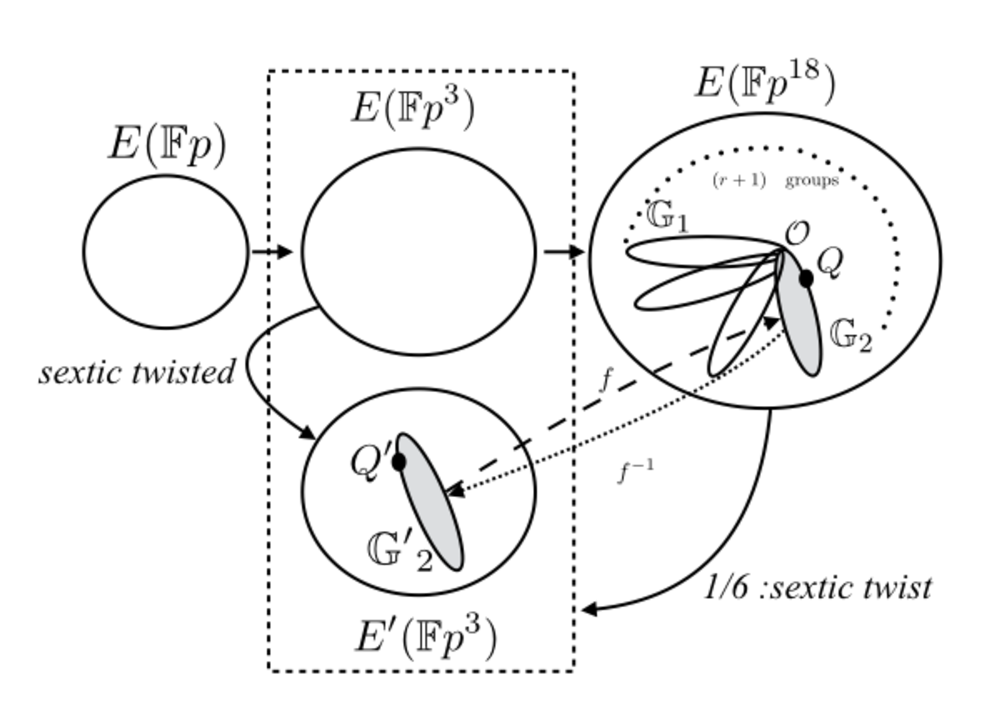
\includegraphics[width=3.5in]{twist.eps}
        \caption{\textit{sextic twist} in KSS curve.}
        \label{fig:sextic}
        \end{figure*}
        Let us consider $E$ is the KSS curve in base field $\FQTH$  and $E'$ is sextic twist of $E'$ given as follows: 
        \begin{eqnarray}
        E:y^2 & = &x^3+b,\\
        E':y^2 & = & x^3+bi, \label{eq:KSS_Twist}
        \end{eqnarray}
        where $b \in \Fp$; $x, y, i \in \FQTH$ and basis element $i$ is the quadratic and cubic non residue in $\FQTH$.
        
        In context of KSS curve, let us consider a rational point $Q\in \g2 \subset E(\F{p}{18})$.
        $Q$ has a  special vector representation with 18 $\Fp$ elements for each $x_Q$ and $y_Q$ coordinates.
        Figure \ref{fig:Q_structure} shows the structure of the coefficients of $Q \in \FQEN$ and its sextic twisted isomorphic rational point $Q' \in \FQTH$ in KSS curve.
        \begin{figure*}
        \centering
        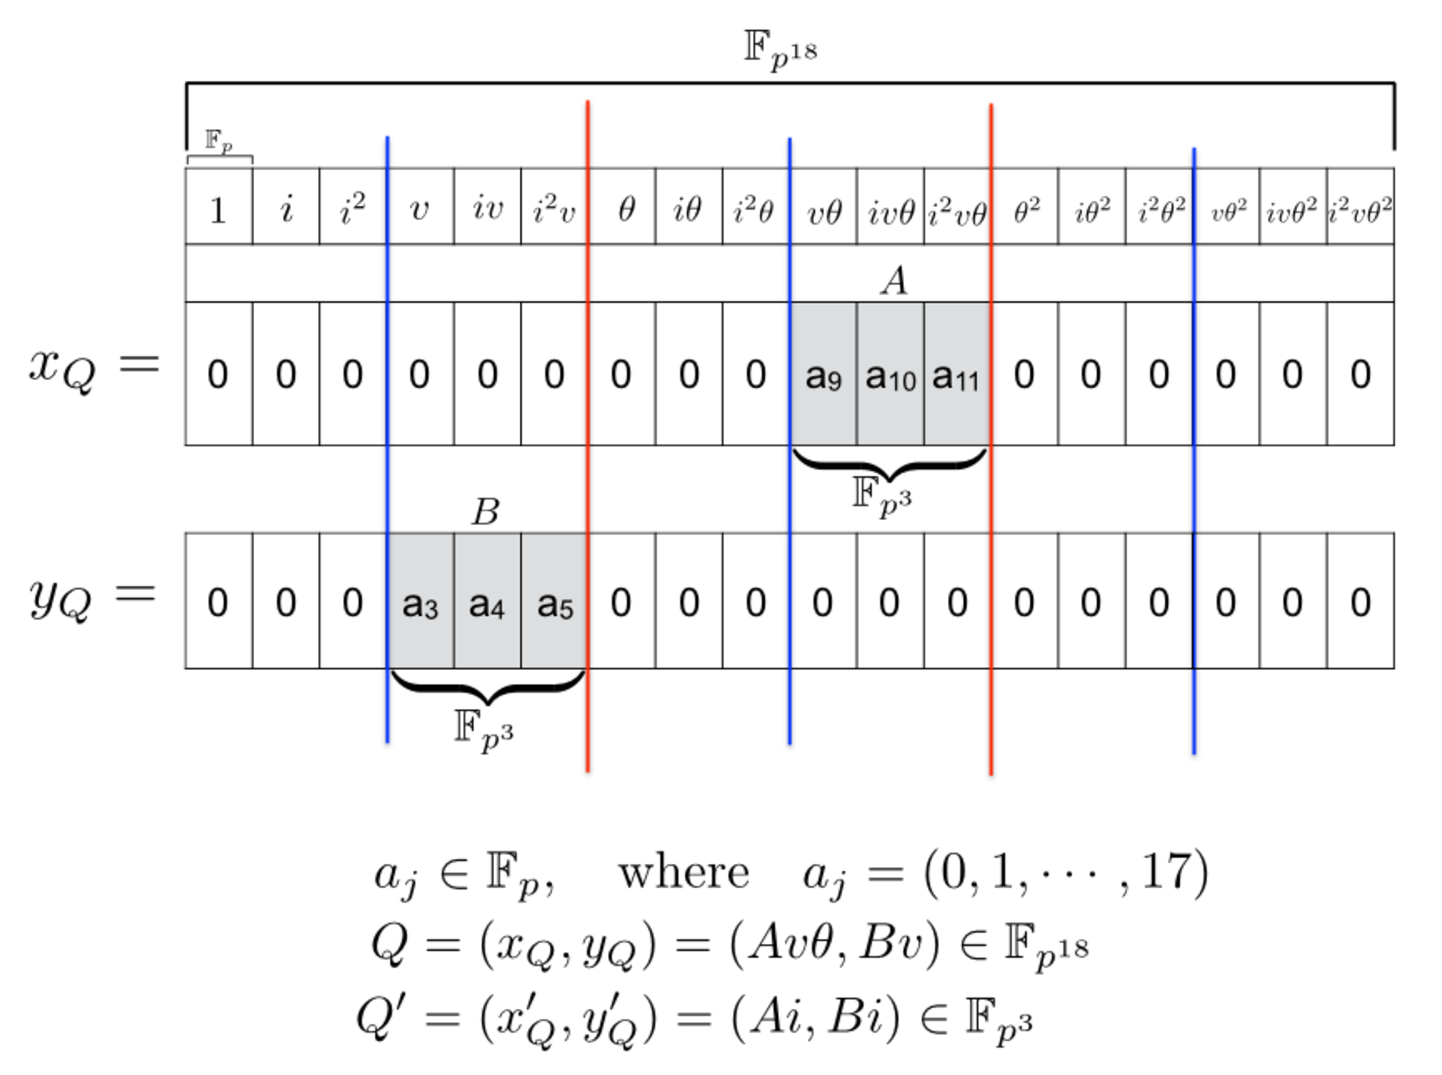
\includegraphics[width=4.5in]{structure.eps}
        \caption{ $Q \in \FQEN$ and its sextic twisted isomorphic rational point $Q' \in \FQTH$ structure in KSS curve.}
        \label{fig:Q_structure}
        \end{figure*}
        Among 18 elements, there are 3 continuous nonzero $\Fp$ elements. The others are zero.
        However the set of these nonzero elements belongs to $\FQTH$. 
        
        This paper considers the mother parameter of KSS curve $u=65$-bit and characteristics $p=511$-bit. In such consideration, $Q$ is given as $Q = (Av\theta, Bv)$,  showed in Figure \ref{fig:Q_structure}, where $A, B \in \FQTH$ and $v$ and $\theta$ are the basis elements of $\F{p}{6}$ and $\FQEN$ respectively. 
        
        Let us consider the sextic twisted isomorphic sub-field rational point of $Q$ as $Q' \in \g2' \subset E'(\F{p}{3})$.
        Considering $x'$ and $y'$ as the coordinates of $Q'$, we can map the rational point $Q = (Av\theta, Bv)$  to the rational point  $Q' = (x',y')$ as follows.
        
        Multiplying both side of \eqref{eq:KSS_Twist} with $\theta^{-6}$, where $i=\theta^6$ and $v = \theta^3$.
        \begin{equation}\label{eq.sextic_div_theta}
        E':  \Big(\frac{y}{\theta^3}\Big)^2  = \Big(\frac{x}{\theta^2}\Big)^3+ b.
        \end{equation}
         $\theta^{-2}$ of  \eqref{eq.sextic_div_theta} can be represented as follows:
         \begin{subequations}
         \begin{eqnarray}
         \theta^{-2} & = & i^{-1}i \theta^{-2}, \nonumber \\
         &  = & i^{-1}\theta^{4}, \label{thta2_4}
         \end{eqnarray}
         and multiplying $i$ with both sides.
         \begin{equation} \label{the4_2}
         \theta^4 = i\theta^{-2}.
         \end{equation}
        Similarly $\theta^{-3}$ can be represented as follows:
         \begin{eqnarray}
         \theta^{-3} & = & i^{-1}i \theta^{-3} \nonumber \\
         &   = & i^{-1}\theta^{3}.\label{thta_3} 
         \end{eqnarray}
         Multiplying $i$ with both sides of \eqref{thta_3} we get $\theta^3$ as,
         \begin{equation}\label{thta_3_3}
         \theta^3 = i\theta^{-3},
         \end{equation}
         \end{subequations}
        
        \subsubsection{$Q$ to $Q'$ mapping}
        Let us represent $Q = (Av\theta, Bv)$  as follows:
        \begin{equation}\label{18_to3}
        Q  =  (A\theta^4, B\theta^3), \quad \text{where $v=\theta^3$}.
        \end{equation}
        From \eqref{the4_2} and \eqref{thta_3_3}, we substitute $ \theta^4 = i\theta^{-2}$ and $\theta^3 = i\theta^{-3}$  in \eqref{18_to3}  as 
        follows:
        \begin{equation}\label{18_to3.1}
        Q  =  (Ai\theta^{-2}, Bi\theta^{-3}),
        \end{equation}
        where $Ai = x'$ and $Bi = y'$ are the coordinates of $Q' =(x',y') \in \FQTH$. Which implies that we can map $Q \in \FQEN$ to $Q' \in \FQTH$ by first selecting the $3$ nonzero $\Fp$ coefficients of each coordinates of $Q$. Then these nonzero $\Fp$ elements form an $\FQTH$ element. After that multiplying the basis element $i$ with that $\FQTH$ element, we get the final $Q' \in \FQTH$. From the structure of $\FQEN$, given in \eqref{eq:KSS_towering}, this mapping has required no expensive arithmetic operation.  Multiplication by the basis element $i$ in $\FQTH$ can be done by 1 bit wise left shifting since $c=2$ is considered for towering in \eqref{eq:KSS_towering}.
        
        \subsubsection{$Q'$ to $Q$ mapping}
         The reverse mapping $Q' =(x',y') \in \FQTH$ to $Q =(Av\theta,Bv) \in \FQEN$ can be obtained as from \eqref{thta2_4}, \eqref{thta_3} and \eqref{eq.sextic_div_theta} as follows:
         \begin{subequations}
         \begin{eqnarray}
         x i^{-1}\theta^{4} & = & Av\theta, \nonumber \\
         y i^{-1}\theta^{3} & = & Bv, \nonumber
         \end{eqnarray}
         \end{subequations}
          which resembles that $Q= (Av\theta, Bv)$. Therefore it means that multiplying $i^{-1}$ with the $Q'$ coordinates and placing the resulted coefficients in the corresponding position of the coefficients in $Q$, will map $Q'$ to $Q$.
        This mapping costs one $\FQTH$ inversion of $i$ which can be pre-computed and one $\Fp$ multiplication.
        
        
        \section{Result Analysis}
        In order to determine the advantage of the proposal, first we have applied the proposed mapping technique to map rational point $Q \in \g2 \subset E(\F{p}{18})$ to its isomorphic point $Q' \in \g2' \subset E'(\F{p}{3})$. After that we performed the scalar multiplication of $Q'$. Then the resulted points are re-mapped to $\g2$ in $\FQEN$. On the other hand we performed scalar multiplication of $Q$ without mapping. In the experiment, 100 scalar numbers of size (about 377-bit) less than order $r$ is generated randomly and then scalar multiplication is calculated for both case. Average value of execution time is considered for comparison.
        The comparative result is shown in Table \ref{tab_opeation}.
        
        In the experiment, mother parameter $u$ is also selected accordingly to find out $\g2$ rational point $Q$. In addition $p=511$-bit is considered, since Scott et al. \cite{kss_param} has proposed the size of the characteristics $p$ to be 508 to 511-bit with order $r$ of 384-bit for 192-bit security level.
        
        In the experiment, KSS curve over $\FQEN$ is given as $y^2 = x^3 + 11$, considering the following parameters
        \begin{eqnarray}
        u & = & 65   \mbox{-bit},  \nonumber \\ 
        p  & = & 511 \mbox{-bit},  \nonumber \\ 
        r  & = & 378 \mbox{-bit} ,\nonumber \\ 
        t  & = & 255  \mbox{-bit}. \nonumber
        \end{eqnarray}
        
        Table \ref{tab1} shows the experiment environment, used to evaluate usefulness of the proposed mapping.  
        \renewcommand{\baselinestretch}{1.5}
        \begin{table*}
        \renewcommand{\arraystretch}{1.3}
        \centering
        \caption{ Computational Environment}
        \label{tab1}
        \begin{tabular}{|c|c|c|}
        \hline 
        • & PC & iPhone6s \\ 
        \hline \hline 
        CPU {\textsuperscript{*}} & \quad 2.7 GHz Intel Core i5 \quad & \quad Apple A9 Dual-core 1.84 GHz \quad \\ 
        \hline 
        Memory & 16 GB & 2 GB \\ 
        \hline 
        OS & Mac OS X 10.11.4 &  iOS 9.3.1 \\ 
        \hline 
        Compiler & gcc 4.2.1 & gcc 4.2.1 \\ 
        \hline 
        \quad Programming Language \quad  & C & Objective-C, C \\ 
        \hline 
        Library & GNU MP \cite{gmp} & GNU MP \\ 
        \hline 
        \multicolumn{3}{l}{\textsuperscript{*}\footnotesize{Only single core is used from two cores.}}\\
        \end{tabular} 
        \end{table*}
        \renewcommand{\baselinestretch}{1.0}
        
        \renewcommand{\baselinestretch}{1.5}
        \begin{table*}
        %\renewcommand{\arraystretch}{1.3}
        \centering
        \caption{ Comparative result of average execution time in [ms] for scalar multiplication}
        \label{tab_opeation}
        \begin{tabular}{|c|c|c|c|}
        \hline
         & \multicolumn{3}{|c|}{\quad Average execution time [ms] comparison \quad} \\ \hline
        & PC & \multicolumn{2}{|c|}{iPhone 6s}  \\ 
         \hline \hline
         & \quad Execution time \quad & \multicolumn{2}{|c|}{\quad Execution time}\\ 
         \hline
        Binary method  with mapping &  $5.4 \times 10^1 $  &  \multicolumn{2}{|c|} { $6.4 \times 10^1$}\\ \hline
        Binary method  without mapping  &  $1.1 \times 10^3$  &  \multicolumn{2}{|c|} { $1.2 \times 10^3$}\\ \hline
        Montgomery ladder  with mapping &  $6.8 \times 10^1 $  &  \multicolumn{2}{|c|} { $8.4 \times 10^1$}\\ \hline
        Montgomery ladder  without mapping  &  $1.5 \times 10^3$  &  \multicolumn{2}{|c|} { $1.6 \times 10^3$}\\ \hline
        \end{tabular} 
        \end{table*}
        \renewcommand{\baselinestretch}{1.0}
        
        Analyzing  Table \ref{tab_opeation}, we can find that scalar multiplication using the proposed  mapping technique  is more than 20 times faster than scalar multiplication without the proposed mapping. It this experiment we used binary method and Montgomery ladder for scalar multiplication in both case. In the previous work of Nogami et al. \cite{nogami}, has showed the procedure to apply Frobenious mapping on twisted elliptic curve for Ate-based pairing. This multiplication can be done more efficiently if skew Frobenius mapping is applied on sextic twisted isomorphic rational point after applying the proposed mapping. 
        
        In the experiment we have used two execution environments; such as PC and iPhone with different CPU frequencies. In both environments only one processor core is utilized. The result also shows that the ratio of execution time of PC and iPhone without mapping  of both methods is about 0.9. On the other hand the ratio of execution time with mapping  of both methods is about 0.8. But the ratio of CPU frequencies of  iPhone and PC is about $1.84 / 2.7 \approx 0.68$. Since PC and iPhone has different processor architectures therefore it's frequency ratio has no relation with the execution time ratio. 
        
        The main focus of this experiment is to evaluate the  acceleration ratio of scalar multiplication by applying the proposed mapping on $\g2$ rational point group of  KSS curve of embedding degree 18. The experiment does not focus on efficiently implementing scalar multiplication for certain environment. There are other pairing friendly curves such as BLS-12, BLS-24 \cite{taxonomy} where sextic twist is available. We will try to apply the proposed mapping on those curves as our future work.
        
        \section{Conclusion and future work}
        In this paper we have proposed mapping procedure of $\g2$ rational point group to its sextic twisted sub-field isomorphic rational point group $\g2'$  and its reverse mapping on KSS curve in context of Ate based pairing. 
        We have also presented the advantages of such mapping by applying binary scalar multiplication and Montgomery ladder on sextic twisted isomorphic rational points in $\g2'$. 
        Then result of  scalar multiplication in $\g2'$ can accelerate the scalar multiplication in $\g2 \subset E(\FQEN)$ by more than 20 times than scalar multiplication of $\g2$ rational point directly in $\FQEN$. In the previous work of Sakemi et al. \cite{sakemi_skew} has proposed skew Frobenious map for $\g1$ rational point defined over BN curve. As a future work we would like to apply such approach on $\g1$ rational point defined over KSS curve. Together with the proposed mapping and the skew Frobenius mapping of $\g1$ will remarkably accelerate scalar multiplication over KSS curve in the context of pairing based cryptography.  
        
        %As a future work we would like to enhance the scalar multiplication in  sub-field isomorphic rational point group by applying Frobenius mapping and some multi-scalar multiplication technique.  
        
        
        \section*{Acknowledgment}
        This work was partially supported by the Strategic Information and Communications R\&D Promotion Programme (SCOPE) of Ministry of Internal Affairs and Communications, Japan.
        
        
          // Merged in IJNC
\chapter{Mapping over Quartic and Sextic twisted KSS Curves}
\label{ch:ijnc2017}
\section{Introduction}
\subsection{Background and Motivation}
In Ate-based pairing with KSS curve,  pairing computations are done in higher degree extension field $\FPK$.
However, KSS curves defined over $\FPEN$ have the sextic twisted isomorphic rational point group defined over $\FPTH$ and KSS curves defined over $\FPSN$ have the quartic twisted  isomorphism over $\FPFR$. 
Therefore we can execute computations in the subfield $\FPKD$ where $d$ is the twist degree. 
Exploiting such a property, different arithmetic operations of Ate-based pairing can be efficiently performed in $\g2$.  
However, performing elliptic curve operations in small extension field brings security issue since they are vulnerable to small subgroup attack \cite{C:LimLee97}. 
Recently Barreto et al. \cite{LC:BCMNPZ15} have studied the resistance of  KSS-18 curves to small subgroup attacks. 
Such resistible KSS-16 curve is also studied by Loubna et al. \cite{EPRINT:GhaFou16b} at 192-bit security level. 
Therefore isomorphic mapping of KSS-18 and KSS-16 curves and implementing arithmetic operation can be done securely in subfield twisted curves for 192-bit security level.
This chapter has mainly focused on isomorphic mapping of $\g2$ rational points from extension field $\FPK$ to its twisted (sextic and quartic) subfield $\FPKD$ and its reverse procedure for both KSS-18 and KSS-16 curves. 

The advantage of such isomorphic mapping is examined by performing scalar multiplication on $\g2 \subset E(\FPK)$ rational point, since scalar multiplication is required repeatedly in cryptographic calculation. 
Three well-known scalar multiplication algorithms are considered for the comprehensive experimental implementation named as binary method, Montgomery ladder and sliding-window method.
This chapter has considered subfield  twisted curve of both  KSS-16 and KSS-18 curve, denoted as $E'$. 
KSS-18 curve $E'$ includes sextic twisted isomorphic rational point group denoted as $\g2' \subset E'(\FPTH)$, whereas  for KSS-16 curve $E'$ contains the quartic twisted  isomorphic rational point group denoted as $\g2' \subset E'(\FPFR)$.
% In KSS curve, $\g2$ is defined over $\FPEN$ whereas its subfield isomorphic group $\g2'$ is defined over $\FPTH$.
Then the proposed mapping technique is applied to map rational points of $\g2$ to its isomorphic $\g2'$. 
After that the scalar multiplication  is performed  in $\g2'$ and then resulted points are re-mapped to $\g2$.

The experiment result shows  that efficiency of  scalar multiplication is increased by more than 20 to 10 times in subfield  twisted curve $E'$ than scalar multiplication in $E(\FPEN)$ and $E(\FPSN)$ respectively without applying the proposed mapping. The mapping and remapping for sextic twisted curves requires one bit wise shifting in $\Fp$, one $\FPTH$ inversion which can be pre-computed and one $\Fp$ multiplication; hence the sextic twisted mapping procedure has no expensive arithmetic operation. On the other hand, quartic twisted mapping requires no arithmetic operation rather it needs some attention since elliptic curve doubling in the twisted curve has a tricky part. The experiment also reveals that sextic twist is preferable since it gives better performance than quartic twist. 
Performance of such isomorphic mapping can be fully realized when it is applied in some pairing-based protocols. 
It is obvious that efficiency of Ate-based pairing protocols depends not only on improved scalar multiplication but also on efficient Miller's algorithm  and final exponentiation implementation. 

\subsection{Related Works}
Pairings are often found in certain extension field $\FPK$, where $p$ is the prime number, also know as characteristics of the field and the minimum extension degree $k$ is called \textit{embedding} degree. 
The rational points $E(\FPK)$ are defined over a certain pairing-friendly curve $E$ of embedded extension field of degree $k$. 
In \cite{PAIRING:AFKMR12}, Aranha et al. have presented pairing calculation for 192-bit security level where  KSS curve of embedding degree 18 is regarded as one of the good candidates for 192-bit security level.
Recently Zhang et al. \cite{INDOCRYPT:ZhaLin12} have shown that the KSS curve of embedding degree 16 are more suitable for 192-bit security level.
Therefore this chapter has considered KSS pairing-friendly curves of embedding degree $k=16$ and $18$.

\subsection{Contribution Outline}
Implementing asynchronous pairing operation on  a certain pairing-friendly non-supersingular curve requires two rational points typically denoted as $P$ and $Q$. 
Generally, $P$ is spotted on the curve  $\EFP$, defined over the prime field $\FP$ and $Q$ is placed in a group of rational points on the curve $E(\FPK)$, defined over $\FPK$, where $k$ is the \textit{embedding degree} of the pairing-friendly curve. 
In the case of  Kachisa-Schaefer-Scott (KSS) pairing-friendly curve family, $k \geq 16$.
Therefore performing pairing calculation on such curves requires calculating elliptic curve operations in higher degree extension field, which is regarded as one of the major bottlenecks to the efficient pairing operation. 
However, there exists a \textit{twisted} curve of $E(\FPK)$, denoted as  $E'(\FPKD)$, where $d$ is the twist degree, on which calculation is faster than the $k$-th degree extension field. 
Rational points group defined over such twisted curve has an isomorphic group in $E(\FPK)$. 
This chapter explicitly shows the mapping  procedure between the isomorphic groups in the context of Ate-based pairing over KSS family of pairing-friendly curves. 
This chapter considers \textit{quartic twist} and \textit{sextic twist} for KSS curve of embedding degree $k =16$ and $k=18$ receptively. 
To evaluate the performance enhancement of isomorphic mapping, this chapter shows the experimental result by comparing the scalar multiplication. 
The result shows that scalar multiplication in $E(\FPKD)$ is 10 to 20  times faster than scalar multiplication in $E(\FPK)$. 
It also shows that sextic twist is faster than the quartic twist for KSS curve when parameter settings for 192-bit security level are considered. 

%In our recent work \cite{ICISC:KONSD16}, presented in ICISC'16 shows the  efficient Miller's algorithm implementation for Ate-based pairings. 
%As a future work, we would also like to apply this isomorphic mapping  in \cite{ICISC:KONSD16} with real pairing-based protocols implementation and evaluate its advantage. 
%
%A part of this work, isomorphic mapping of KSS curve of embedding degree 18, has been presented at CANDAR'16 \cite{self_candar}.
%In this chapter, we have additionally considered quartic twist for  KSS-16 curve. 
%We have chosen the parameter of KSS-16 curve from \cite{EPRINT:GhaFou16b} for 192-bit security.
%The quartic twist is also compared with sextic twist of KSS-18 curve with detailed implementation procedure. 
%The main focus of this chapter is to demonstrate the details implementation procedure of sextic and quartic twist on KSS-18 and KSS-16 curve respectively at 192-bit security level. 
%
%The rest of the chapter is organized as follows: section 2  briefly overviews the fundamentals of elliptic curve arithmetic, scalar multiplication and the construction of  KSS curves over $\FPEN$ and $\FPSN$ extension field. The rational point groups for asynchronous pairing and the twist (quartic, sextic) property is also discussed in this section.  
%In section 3, the proposed isomorphic mapping technique between rational point $Q$ and $Q'$ over the twisted KSS curves is described in details. 
%The experimental result is presented in section 4, which shows that scalar multiplication on $\g2$ point can be accelerated by 10 to 20 times by applying the proposed mapping technique in both KSS-16 and KSS-18. The result also shows that the sextic twist of KSS-18 is faster than the quartic twist of the KSS-16 curve. 
%The chapter concludes in section 5  with an outline of future enhancement.

\section{Fundamentals}
Most of the fundamentals related to this chapter is already discussed in the previous chapters.
In this section we briefly recall KSS family of pairing-friendly curves and twisted property of KSS curve.

\subsection{Kachisa-Schaefer-Scott (KSS) Curve Family}
 In \cite{EPRINT:KacSchSco07}, Kachisa, Schaefer, and Scott proposed a family of non super-singular Brezing-Weng pairing-friendly elliptic curves of embedding degree $k = \left\lbrace16, 18, 32, 36, 40\right\rbrace$, using elements in the cyclotomic field. Similar to other pairing-friendly curves,  \textit{characteristic} $p$, \textit{Frobenius trace} $t$ and \textit{order} $r$ of these curves are given systematically by using an integer variable also known as mother parameter. In what follows, this chapter considers two curves of this family named as \textit{KSS-16} of embedding degree $k =16$  and \textit{KSS-18} of $k=18$. 

KSS-18 curve, defined over $\FPEN$, is given by the following equation
\begin{equation}\label{eq:KSS_curve_18_chap_ijnc2017_chap_ijnc2017}
E/\FPEN:Y^2=X^3+b, \quad \mbox{$b \in \Fp$ and $b \neq 0$ },
\end{equation}
where  $X,Y \in \FPEN$. KSS-18 curve is parameterized by an integer variable $u$ as follows:
\begin{subequations}
\begin{eqnarray}
p(u)  &= &(u^8 +5u^7 +7u^6 +37u^5 +188u^4 +259u^3 + 343u^2 +1763u \nonumber \\
& &   +2401)/21,              \label{eq:kss_char_chap_ijnc2017} \\
r(u) & =&  (u^6 + 37u^3 + 343)/343, \label{eq:kss_degree_chap_ijnc2017}  \\
t(u) &=&  (u^4 + 16u + 7)/7. \label{eq:kss18_trace_chap_ijnc2017} 
\end{eqnarray}
\end{subequations} 
The necessary condition for $u$ is $u \equiv 14$ (mod $42$) and the $\rho$ value is $\rho = (\log_2 p/\log_2 r) \approx 1.33$.

On the other hand, KSS-16 curve is defined over $\FPSN$, represented by the following equation
\begin{equation}\label{eq:KSS_16_trace_chap_ijnc2017}
E/\FPSN:Y^2=X^3+aX, \quad \mbox{($a \in \Fp$) and  $a \neq 0$},
\end{equation}
 where $X,Y \in \FPSN$. Its characteristic $p$, Frobenius trace $t$ and order $r$ are given the integer variable $u$ as follows:
\begin{subequations}
\begin{eqnarray}
p(u) &= & (u^{10} +2u^9 +5u^8 +48u^6 +152u^5 +240u^4 +625u^2 +2398u \nonumber \\
&& +3125)/980,  \\\label{eq:kss_16_char_trace_chap_ijnc2017}
r(u) &= & u^8 +48u^4 +625,\label{eq:kss_16_degree_chap_ijnc2017}  \\
t(u) &=& (2u^5 +41u+35)/35, \label{eq:kss_16_trace_chap_ijnc2017} 
\end{eqnarray}
\end{subequations} 
where $u$ is such that $u \equiv 25$ or $45$ (mod $70$) and the $\rho$ value is $\rho = (\log_2 p/\log_2 r) \approx 1.25$.

%KSS-16 and KSS-18 both curves are good candidate for realizing 128-bit security 
%
%In the previous work of  Aranha et al. \cite{PAIRING:AFKMR12} and Scott et al. \cite{IMA:Scott11} has mentioned that the size of the characteristics $p$ to be 508 to 511-bit with order $r$ of 384-bit  for 192-bit security level.  
%Therefore this chapter used parameter settings according to the suggestion of \cite{PAIRING:AFKMR12} for 192 bit security on KSS curve in the simulation implementation. In the recent work, Kim et al. \cite{C:KimBar16} has suggested to update the key sizes in pairing-based cryptography due to the  development of new discrete logarithm problem over finite field. The parameter settings used in this chapter doesn't completely end up at the 192 bit security level according to \cite{C:KimBar16}. However, the parameter settings used in this chapter in order to show the resemblance of the



\subsection{Extension Field Construction for KSS Curves}
Pairing-based cryptography requires  performing the arithmetic operation in extension fields of degree $k \geq 6$ \cite{Silverman}. 
We recall \secref{sec:ch:icisc:kss18curve} for the extension field construction of KSS-18 curve.
Since this chapter uses two curves of different extension degree, therefore, the construction process of $\FPEN$ and $\FPSN$ are represented in the following as a tower of subfields. 

\subsubsection{Towering of \texorpdfstring{$\FPEN$}{} Extension Field}
Let $3|(p-1)$, where $p$ is the characteristics of KSS-18 and $c$ is a quadratic and cubic non residue in $\Fp$. In the context  of KSS-18, where $k=18$, $\FPEN$ is constructed as tower field with irreducible binomial as follows:
\begin{equation}\label{eq:KSS-18_towering_chap_ijnc2017}
\begin{cases}
\F{p}{3} = \F{p}{}[i]/(i^3-c),  \\ 
\F{p}{6} = \F{p}{3}[v]/(v^2-i),  \\ 
\F{p}{18} = \F{p}{6}[\theta]/(\theta^3-v). \\ 
\end{cases}
\end{equation}
Here $c = 2$ is considered to be the best choice for efficient extension field arithmetic.
From the above towering construction we can find that $i=v^2=\theta^6$, where $i$ is the basis element of the base extension field $\FPTH$. 

\subsubsection{Towering of \texorpdfstring{$\FPSN$}{} Extension Field}
Let the characteristics $p$ of KSS-16 is such that  $4|(p-1)$  and $z$ is a quadratic non residue in $\Fp$. By using irreducible binomials, $\FPSN$ is constructed for KSS-16 curve  as follows:
\begin{equation}\label{eq_KSS16_towering_towering_chap_ijnc2017}
\begin{cases}
\F{p}{2} = \F{p}{}[\alpha]/(\alpha^2-z),  \\ 
\F{p}{4} = \F{p}{2}[\beta]/(\beta^2-\alpha),  \\ 
\F{p}{8} = \F{p}{4}[\gamma]/(\gamma^2-\beta), \\ 
\F{p}{16} = \F{p}{8}[\omega]/(\omega^2-\gamma), \\ 
\end{cases}
\end{equation}
Here $z = 11$ is chosen along with the value of mother parameter $u$ as given in \tbref{table_KSS16_param_chap_ijnc2017}.

\subsection{\texorpdfstring{\g1}{G1}, \texorpdfstring{\g2}{G2} and \texorpdfstring{\g3}{G3} Groups} In the context of pairing-based cryptography, especially on KSS curve, two addititive rational point groups $\g1, \g2$ and a multiplicative group $\mathbb{G}_3$ of order $r$ are considered. From \cite{PAIRING:MANS13},  $\g1$, $\g2$ and $\g3$ are defined as follows:
\begin{eqnarray}\label{eq:groupsg1g2g3_chap_ijnc2017}
\g1 & = &  E(\F{p}{k}) [r] \cap \text{Ker}(\pi_p - [1]), \nonumber \\
\g2 & = &  E(\F{p}{k}) [r] \cap \text{Ker}(\pi_p - [p]), \nonumber \\
\g3 & = & \mF{p}{k}/(\mF{p}{k})^r, \nonumber
\end{eqnarray}
\begin{equation}
\xi : \g1 \times \g2 \rightarrow \g3,
\end{equation}
where $\xi$ denotes Ate pairing. In the case of KSS curves, the above $\g1$ is just $E(\FP)$. In what follows, rest of this chapter considers 
 $P \in \g1 \subset E(\FP)$ and  $Q \in \g2$ where  $\g2$ is a subset of $E(\FPSN)$ and $E(\FPEN)$ for KSS-16 and KSS-18 curves respectively. 

\subsection{Twist of KSS Curves}
Let us consider performing an asynchronous type of pairing operation on KSS curves.  Let it be the Ate pairing $\xi(P,Q)$, one of asynchronous variants. $P$  is defined over the prime field $\FP$ and  $Q$ is typically placed on the $k$-th degree extension field $\FPK$ on the defined KSS curve. There exists a \textit{twisted curve} with a group of rational points of order $r$ which are isomorphic to the group where rational point $Q \in  E(\FPK)$  belongs to. This subfield isomorphic rational point group includes a twisted isomorphic point of $Q$, typically denoted as $Q' \in E'(\FPKD)$, where $k$ is the embedding degree and $d$ is the twist degree.  

Since points on the twisted curve are defined over a smaller field than $\FPK$, therefore ECA and ECD becomes faster. 
However, when required in the pairing calculation such as  for line evaluation  they can be quickly mapped to a point on $E(\FPK )$. 
Defining such mapping and re-mapping techniques is the main focus of this  chapter. Since the pairing-friendly KSS-16 \cite{EPRINT:KacSchSco07} curve has CM discriminant of $D = 1$ and $4|k$, therefore quartic twist is available. For sextic twist, the curve should have $D = 3$ and $6|k$, which exists in KSS-18.

\subsubsection{Sextic Twist of KSS-18 Curve}
%When the embedding degree $k = 2e$, where $e$ is positive integer, from \eqref{ec_curve} the quadratic twisted elliptic curve $E'_2$ is given as follows:
%\begin{equation}\label{eq:quad_twist}
%E'_2:y^2=x^3+az^{-2}+bz^{-3}, \quad a,b \in \F{p},
%\end{equation}
%where $z$ is a quadratic non residue in $\F{p}{e}$. Then, between $E'_2(\F{p}{e})$ and $E(\F{p}{2e})$, the following isomorphism is given.
%\begin{eqnarray}
%\psi_2 : \begin{cases}
%E'_2(\F{p}{e}) \rightarrow E(\F{p}{2e}),\\
%(x,y) \quad \mapsto (xz,yz^{3/2}),
%\end{cases}
%\end{eqnarray}
%where $x, y$ are the coordinates of rational point. In this case, $E'_2$ is called \textit{quadratic-twisted} curve. In the same, 

When the embedding degree $k = 6e$, where $e$ is positive integer, \textit{sextic} twist  is given as follows:
\begin{eqnarray}
E:  \quad y^2 & = & x^3+b, \quad b \in \Fp, \\
E'_6: \quad y^2 & =  & x^3+b\nu^{-1},
\end{eqnarray}  
where $\nu$ is a quadratic and cubic non residue in $E(\F{p}{e})$ and $3|(p^e-1)$.  For KSS-18 curve $e=3$. Isomorphism between $E'_6(\F{p}{e})$ and $E(\F{p}{6e})$, is given as follows:
\begin{eqnarray}
\psi_6 : \begin{cases}
E'_6(\F{p}{e}) \rightarrow E(\F{p}{6e}),\\
(x,y) \quad \mapsto (x\nu^{1/3},y\nu^{1/2}).
\end{cases}
\end{eqnarray}

%In the context of Ate-based pairing for KSS curve of embedding degree 18, sextic twist is considered to be the most efficient. This chapter considers mapping of sextic twisted subfield isomorphic group of $\FPEN$. 

\subsubsection{Quartic Twist of KSS-16 Curve}
\label{sec:ch:ijnc:kss16twist}
The quartic twist of KSS-16 curve is given as  follows:
\begin{eqnarray}
E:  \quad y^2 & = & x^3+ax, \quad a \in \Fp, \\
E'_4: \quad y^2 & =  & x^3+a\sigma^{-1}x,
\end{eqnarray}  
where $\sigma$ is a quadratic non residue in $E(\F{p}{4})$ and $4|(p-1)$.  The Isomorphism between $E'_4(\F{p}{4})$ and $E(\F{p}{16})$, is given as follows:
\begin{eqnarray}
\psi_4 : \begin{cases}
E'_4(\F{p}{4}) \rightarrow E(\F{p}{16}),\\
(x,y) \quad \mapsto (x\sigma^{1/2},y\sigma^{3/4}).
\end{cases}
\end{eqnarray}

\section{Isomorphic Mapping between \texorpdfstring{$Q$}{Q} and \texorpdfstring{$Q'$}{Q'}}
This section introduces the derived mapping procedure of $\g2$ rational point group to its twisted (quartic and  sextic) isomorphic group $\g2'$ for Ate-based pairing for the considered KSS curves. 
The idea of isomorphic mapping for KSS-18  is already defined in  \secref{sec:ch:ieice2016:mappingQtoQprime} of \chref{Chapter_IEICE}. 
In this section we recall this mapping to for more comprehensive reading along with the newly introduced idea of aquatic twist.

\subsection{Sextic twisted Isomorphic Mapping between \texorpdfstring{$Q \in \g2 \subset E(\FPEN)$}{} and \texorpdfstring{$Q' \in \g2' \subset E'(\FPTH)$}{}}
Figure \ref{fig:sextickss18_chap_ijnc2017} shows an overview of sextic twisted curve $E'(\FPTH)$ of $E(\FPEN)$.
\begin{figure*}
\centering
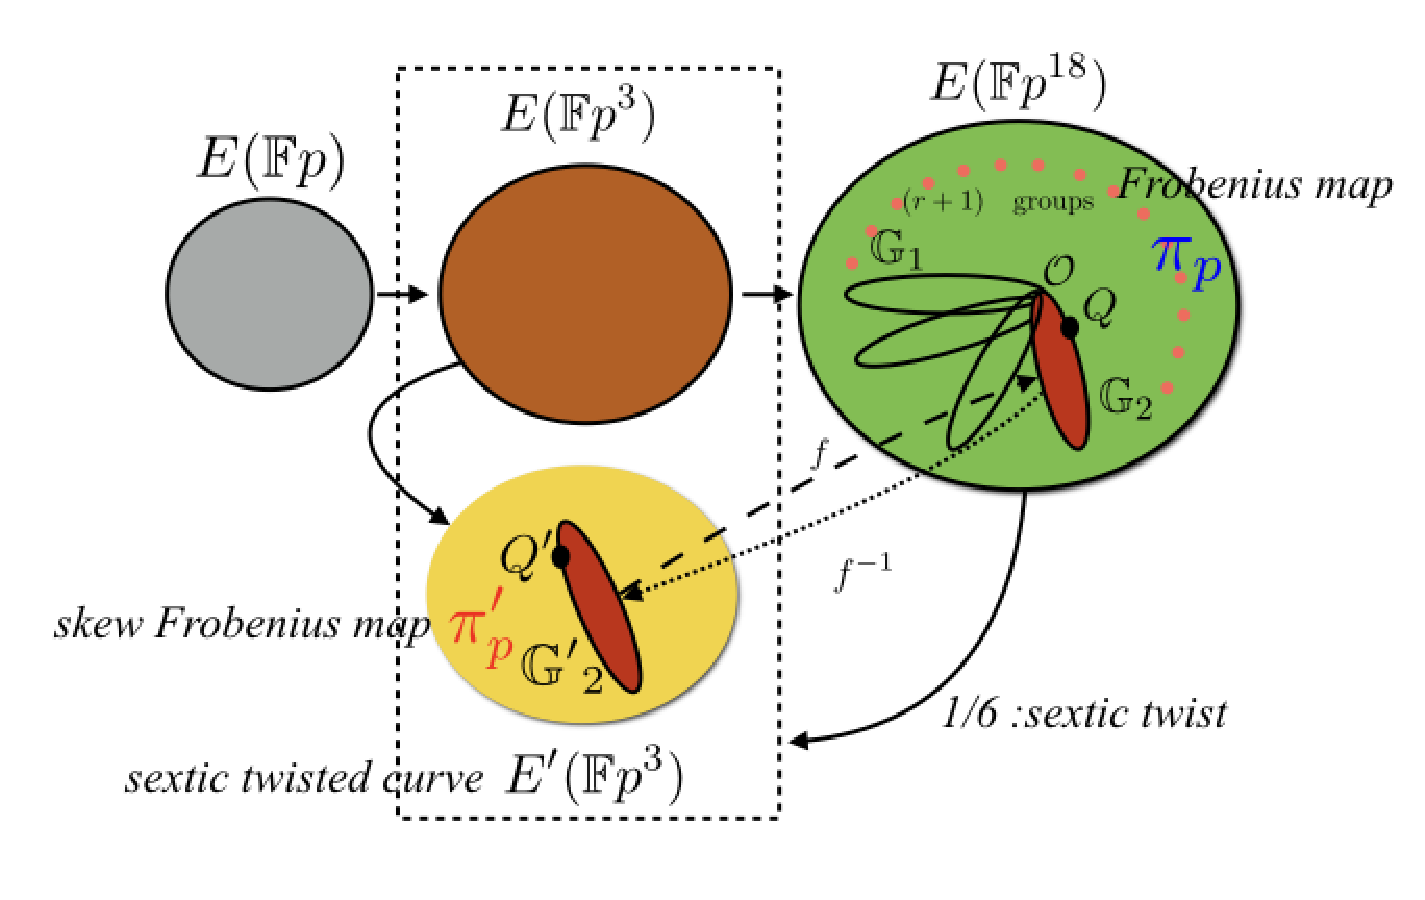
\includegraphics[width=3.5in]{sfm.eps}
\caption{\textit{sextic twist} in KSS-18 curve.}
\label{fig:sextickss18_chap_ijnc2017}
\end{figure*}

Let us consider $E$ be the KSS-18 curve in base field $\FPTH$  and $E'$ is sextic twist of $E'$ given as follows: 
\begin{eqnarray}
E:y^2 & = &x^3+b,\\
E':y^2 & = & x^3+bi, \label{eq:KSS18_Twist_chap_ijnc2017}
\end{eqnarray}
where $b \in \Fp$; $x, y, i \in \FPTH$ and basis element $i$ is the quadratic and cubic non residue in $\FPTH$.

In the context of KSS-18 curve, let us consider a rational point $Q\in \g2 \subset E(\F{p}{18})$.
$Q$ has a  special vector representation with 18 $\Fp$ elements for each $x_Q$ and $y_Q$ coordinate.
Figure \ref{fig:Q_structureKSS18_chap_ijnc2017} shows the structure of the coefficients of $Q \in \FPEN$ and its sextic twisted isomorphic rational point $Q' \in \FPTH$ in KSS-18 curve.
\begin{figure*}
\centering
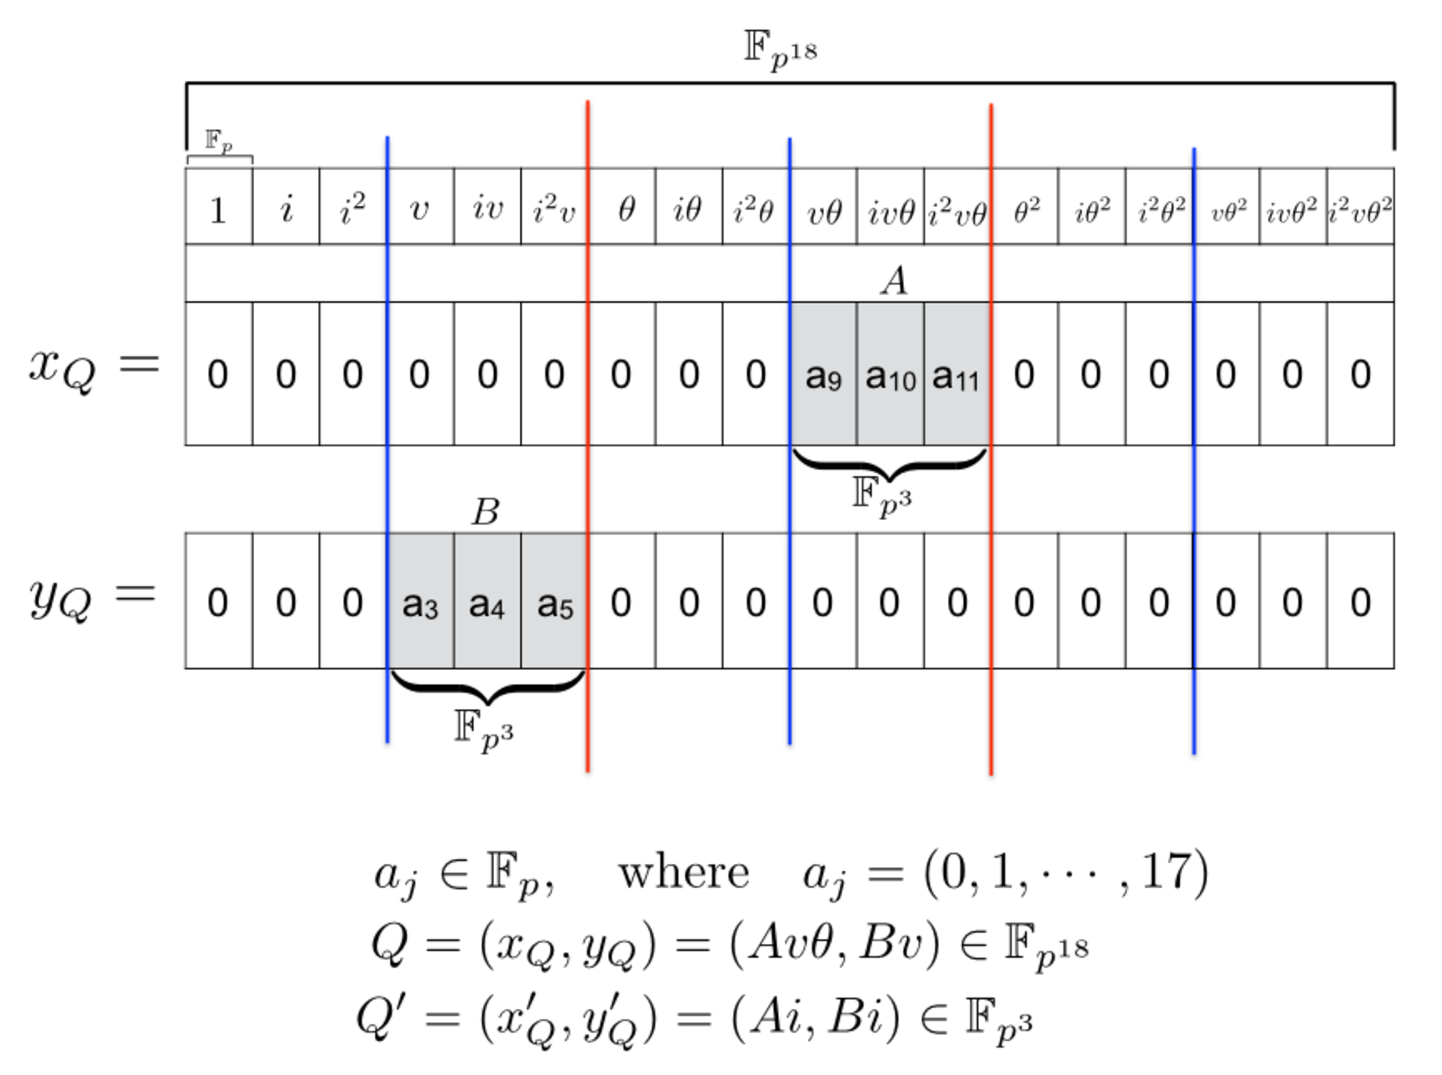
\includegraphics[width=4.5in]{structure.eps}
\caption{ $Q \in \FPEN$ and its sextic twisted isomorphic rational point $Q' \in \FPTH$ structure in KSS-18 curve.}
\label{fig:Q_structureKSS18_chap_ijnc2017}
\end{figure*}
Among 18 elements, there are 3 continuous nonzero $\Fp$ elements. The others are zero.
However, the set of these nonzero elements belongs to a $\FPTH$ field. 

This chapter considers parameter given in \tbref{table_KSS18_param_chap_ijnc2017} for KSS-18 curve where mother parameter $u=65$-bit and characteristics $p=511$-bit. In such consideration, $Q$ is given as $Q = (Av\theta, Bv)$,  showed in Figure \ref{fig:Q_structureKSS18_chap_ijnc2017}, where $A, B \in \FPTH$ and $v$ and $\theta$ are the basis elements of $\F{p}{6}$ and $\FPEN$ respectively. 

Let us consider the sextic twisted isomorphic subfield rational point of $Q$ as $Q' \in \g2' \subset E'(\F{p}{3})$.
Considering $x'$ and $y'$ as the coordinates of $Q'$, we can map the rational point $Q = (Av\theta, Bv)$  to the rational point  $Q' = (x',y')$ as follows.

Multiplying both side of \eqref{eq:KSS18_Twist_chap_ijnc2017} with $\theta^{-6}$, where $i=\theta^6$ and $v = \theta^3$.
\begin{equation}\label{eq:sextic_div_thetaKSS18_chap_ijnc2017}
E':  \Big(\frac{y}{\theta^3}\Big)^2  = \Big(\frac{x}{\theta^2}\Big)^3+ b.
\end{equation}
 $\theta^{-2}$ of  \eqref{eq:sextic_div_thetaKSS18_chap_ijnc2017} can be represented as follows:
 \begin{subequations}
 \begin{eqnarray}
 \theta^{-2} & = & i^{-1}i \theta^{-2}, \nonumber \\
 &  = & i^{-1}\theta^{4}, \label{eq:thta2_4KSS18_chap_ijnc2017}
 \end{eqnarray}
 and multiplying $i$ with both sides.
 \begin{equation} \label{eq:tthe4_2KSS18_chap_ijnc2017}
 \theta^4 = i\theta^{-2}.
 \end{equation}
Similarly $\theta^{-3}$ can be represented as follows:
 \begin{eqnarray}
 \theta^{-3} & = & i^{-1}i \theta^{-3}, \nonumber \\
 &   = & i^{-1}\theta^{3}.\label{eq:theta_3KSS18_chap_ijnc2017} 
 \end{eqnarray}
 Multiplying $i$ with both sides of \eqref{eq:theta_3KSS18_chap_ijnc2017} we get $\theta^3$ as,
 \begin{equation}\label{eq:thta_3_3KSS18_chap_ijnc2017}
 \theta^3 = i\theta^{-3},
 \end{equation}
 \end{subequations}

\subsubsection{\texorpdfstring{$Q$}{} to \texorpdfstring{$Q'$}{} Mapping in KSS-18}
Let us represent $Q = (Av\theta, Bv)$  as follows:
\begin{equation}\label{eq:map18_to3KSS18_chap_ijnc2017}
Q  =  (A\theta^4, B\theta^3), \quad \text{where $v=\theta^3$}.
\end{equation}
From \eqref{eq:tthe4_2KSS18_chap_ijnc2017} and \eqref{eq:thta_3_3KSS18_chap_ijnc2017}, we substitute $ \theta^4 = i\theta^{-2}$ and $\theta^3 = i\theta^{-3}$  in \eqref{eq:map18_to3KSS18_chap_ijnc2017}  as 
follows:
\begin{equation}\label{eq:map18_to3KSS18_chap_ijnc2017.1}
Q  =  (Ai\theta^{-2}, Bi\theta^{-3}),
\end{equation}
where $Ai = x'$ and $Bi = y'$ are the coordinates of $Q' =(x',y') \in \FPTH$. Which implies that we can map $Q \in \FPEN$ to $Q' \in \FPTH$ by first selecting the $3$ nonzero $\Fp$ coefficients of each coordinate of $Q$. Then these nonzero $\Fp$ elements form a $\FPTH$ element. After that multiplying the basis element $i$ with that $\FPTH$ element, we get the final $Q' \in \FPTH$. From the structure of $\FPEN$, given in \eqref{eq:KSS-18_towering_chap_ijnc2017}, this mapping has required no expensive arithmetic operation.  Multiplication by the basis element $i$ in $\FPTH$ can be done by 1 bitwise left shifting since $c=2$ is considered for towering in \eqref{eq:KSS-18_towering_chap_ijnc2017}.

\subsubsection{\texorpdfstring{$Q'$}{} to \texorpdfstring{$Q$}{} Mapping in KSS-18}
 The reverse mapping $Q' =(x',y') \in \FPTH$ to $Q =(Av\theta,Bv) \in \FPEN$ can be obtained as from \eqref{eq:thta2_4KSS18_chap_ijnc2017}, \eqref{eq:theta_3KSS18_chap_ijnc2017} and \eqref{eq:sextic_div_thetaKSS18_chap_ijnc2017} as follows:
 \begin{subequations}
 \begin{eqnarray}
 x i^{-1}\theta^{4} & = & Av\theta, \nonumber \\
 y i^{-1}\theta^{3} & = & Bv, \nonumber
 \end{eqnarray}
 \end{subequations}
  which resembles that $Q= (Av\theta, Bv)$. Therefore it means that multiplying $i^{-1}$ with the $Q'$ coordinates and placing the resulted coefficients in the corresponding position of the coefficients in $Q$, will map $Q'$ to $Q$.
This mapping costs one $\FPTH$ inversion of $i$ which can be pre-computed and one $\Fp$ multiplication.

\subsection{Quartic Twisted Isomorphic Mapping}
\label{sec:ch:ijnc:kss16twist_isomorphicmap}

For quartic twisted mapping first we need to obtain certain ration point  $Q \in \g2 \subset E(\FPSN)$ of subgroup order $r$. 
One necessary condition for obtaining such $Q$ is $r^2 \mid \#E(\FPSN)$, where $\#E(\FPSN)$ is the number of rational points in $E(\FPSN)$.  But it is carefully observed that $\#E(\FPSN)$ is not divisible by $r^2$ when $r$ is given by \eqref{eq:kss_16_degree_chap_ijnc2017}.
 Therefore polynomial of $r$, given in \cite{EPRINT:KacSchSco07} is divided as follows:
\begin{equation}
r(u) =  (u^8 +48u^4 +625)/61250,
\end{equation}
to make it dive  $\#E(\FPSN)$ completely.

Let us consider the rational point $Q \in \g2 \subset E(\FPSN)$ and its quartic twisted rational point $Q' \in \g2 \subset E'(\FPFR)$. Rational point $Q$ has a special vector representation given in  \tbref{table:QKSS-16_chap_ijnc2017}.

\renewcommand{\baselinestretch}{1.5}
\begin{table}[ht] 
	\begin{center}
		\caption{Vector representation of $Q = (x_Q,y_Q) \in \FPSN$}
		\resizebox{\columnwidth}{!}{
		\begin{tabular}{|c|c|c|c|c|c|c|c|c|c|c|c|c|c|c|c|c|c|}
			\hline 
			   & 1 & $\alpha$ & $\beta$ & $\alpha \beta$ & $\gamma$ & $\alpha \gamma$ & $\beta \gamma$ & $\alpha \beta \gamma$ & $\omega$ & $\alpha \omega$ & $ \beta \omega$ & $\alpha \beta \omega$ & $\gamma \omega$ & $\alpha \gamma \omega$ &$ \beta \gamma \omega$ & $\alpha \beta \gamma \omega$\\ \hline 
			$x_Q$ & 0 & 0 & 0 & 0 & $n_4$ & $n_5$ &$ n_6$ & $n_7$ & 0 & 0 & 0 & 0 & 0 & 0 & 0& 0\\ \hline 
			$y_Q$ & 0 & 0 & 0 & 0 & 0 & 0 & 0 & 0 & 0 & 0 & 0 & 0 & $n_{12}$ & $n_{13}$ & $n_{14}$ & $n_{15}$\\\hline 
		\end{tabular}\label{table:QKSS-16_chap_ijnc2017}
	}
	\end{center}
\end{table}
\renewcommand{\baselinestretch}{1.0}

From  \tbref{table:QKSS-16_chap_ijnc2017} co-ordinates of  $Q = (x_Q,y_Q) \in \FPEN$ is obtained as $Q = (x_Q,y_Q) = (\gamma x_{Q'}, \omega \gamma y_{Q'}) $ where $x_{Q'},y_{Q'}$ are the co-ordinates of the rational point $Q'$ in the twisted curve. Now let's find the twisted curve of \eqref{eq:KSS_16_trace_chap_ijnc2017} in $\FPFR$ as follows:
\begin{eqnarray}
(\omega\gamma y_{Q'} )^2 & = & (\gamma x_{Q'})^3 + a (\gamma x_{Q'}), \nonumber \\
\gamma \beta y_{Q'}^2 & = & \gamma \beta x_{Q'}^3 + a \gamma x_{Q'}, \nonumber \\
y_{Q'}^2 & = & x_{Q'}^3 + a \beta^{-1}x_{Q'}, \quad  \mbox{multiplying $(\gamma \beta)^{-1}$ both sides.}
\end{eqnarray}
 The twisted curve of $E'$ is obtained as $y^2  =  x^3 + a \beta^{-1}x$ where $\beta$ is the basis element in $\FPFR$. 
 There is a tricky part that needs attention when calculating the ECD in $E'(\FPFR)$ presented in the following equation.
 \begin{equation}
 \lambda =   (3x_{Q'}^2+\textbf{a})(2y_{Q'})^{-1},
 \end{equation}
 where $\textbf{a} \in \FPFR$, since $\textbf{a} = a \beta^{-1}$ and $\beta \in \FPFR$. The calculation of $\textbf{a} = a \beta^{-1}$
 is given as follows:
 \begin{eqnarray}
  a \beta^{-1} & = & (a + 0\alpha + 0 \beta + 0 \alpha \beta) \beta ^{-1}, \nonumber \\
  & & = z^{-1} a \alpha \beta \quad \mbox{where $\alpha^2 = z$}
 \end{eqnarray}
 
 Now let us denote the quartic mapping as follows:
 \begin{equation}
Q = (x_Q,y_Q) = (\gamma x_{Q'}, \omega \gamma y_{Q'}) \in \g2 \subset E(\FPSN)   \longmapsto  Q' = (x_{Q'},y_{Q'}) \in \g2'  \subset E'(\FPFR).  \nonumber
 \end{equation}
 
 For mapping from $Q$ to $Q'$ no extra calculation is required. By picking the non-zero coefficients  of $Q$ and placing it to the corresponding basis position is enough to get $Q'$. Similarly, re-mapping from $Q'$ to $Q$  can also be done without any calculation rather multiplying with basis elements.  

\section{Result Analysis}
The main focus of this proposed mapping is to find out the isomorphic mapping of two well-known pairing-friendly curves, KSS-16 and KSS-18. In order to determine the advantage of the proposal, this chapter has implemented 3 well-known elliptic curve scalar multiplication method named as the binary method, Montgomery ladder method, and sliding-window method.

For the experiment first we have applied the proposed mapping technique to map rational point $Q \in \g2 \subset E(\F{p}{k})$ to its isomorphic point $Q' \in \g2' \subset E'(\FPKD)$ in both KSS curves. After that we performed the scalar multiplication of $Q'$. Then the resulted points are re-mapped to $\g2$ in $\FPK$. Lets define this strategy as \textit{\textbf{with mapping}}.
On the other hand, we have performed scalar multiplication of $Q$ without mapping which is denoted as \textit{\textbf{w/o mapping}}.

In the experiment, after many careful searches, the mother parameter $u$ is selected to find out $\g2$ rational point $Q$ for KSS-18 curve. On the other hand, for KSS-16 curve, parameters are given by Loubna et al. \cite{EPRINT:GhaFou16b}.
In pairing-based cryptosystems, both KSS-16 and KSS-18 are regarded as good candidates for implementing 192-bit security.
Therefore, while choosing parameters for the experiment, this chapter has adapted 192-bit security level. 
But the main focus of this chapter is not to find out efficient parameters for certain security levels. 
The main purpose of the selected the parameters is to compare the twisted isomorphic mappings on the nominated curves at standard security levels. 

 \tbref{table_KSS18_param_chap_ijnc2017} and  \tbref{table_KSS16_param_chap_ijnc2017} show the parameters used in the experiment.
  \tbref{table_comenv_twist_chap_ijnc2017} shows the experiment environment, used to evaluate the usefulness of the proposed mapping.  
In the experiment, 100 scalar numbers of size less than order $r$ is generated randomly and then scalar multiplication is calculated for both cases. Average value of execution time in [ms] is considered for comparison. 
 \tbref{table_additional_twist_chap_ijnc2017} shows the  settings considered during the experiment.
 The comparative result is shown in  \tbref{table_opeationcomp_chap_ijnc2017}.

Parameter of KSS curves are given in decimal value used for evaluating the mapping efficiency in the experiment.

	\renewcommand{\arraystretch}{1.2}{
\begin{table}[ht]
	\centering
	\caption{KSS-18 Parameters}
	\label{table_KSS18_param_chap_ijnc2017}
	\resizebox{\columnwidth}{!}{
	\begin{tabular}{|l|l|l|}
		\hline
		$y^2 =$ & $x^3 + 11$                                                                                                                                                                                                 & bit size \\ \hline
		$u =$   & $23058430092138432950$                                                                                                                                                                                     & 65       \\ \hline
		$p=$    & \begin{tabular}[c]{@{}l@{}}$380556013753003852484338059727997572538865139076812$\\ $970560732143111526346817611942575176069026109216559$\\ $8021019048849831001675531254097766654664544068613131$\end{tabular} & 511      \\ \hline
		$r=$    & \begin{tabular}[c]{@{}l@{}}$4382120271066581232104344084955320374849908135951851$\\ $5268755202336574860904936668100704293777799119708528$\\ $7495125001$\end{tabular}                                         & 378      \\ \hline
		$t=$    & \begin{tabular}[c]{@{}l@{}}$4038507576637353290391809403638366577735736214369368$\\ $5385569578231170388739601$\end{tabular}                                                                                 & 255      \\ \hline
	\end{tabular}
}
\end{table}
}

\begin{table}[ht]
	\caption{KSS-16 Parameters}
	\label{table_KSS16_param_chap_ijnc2017}
	\resizebox{\columnwidth}{!}{
	\begin{tabular}{|l|l|l|}
		\hline
		$y^2 =$ & $x^3 + 17x$                                                                                                                                                                                               & bit size \\ \hline
		$u =$   & $1266366845779935$                                                                                                                                                                                        & 51       \\ \hline
		$p=$    & \begin{tabular}[c]{@{}l@{}}$108235379323342249430403752839634417782861787922010$\\ $5831937449880701267192580688017668298801139820714475$\\ $1031509661694254867934067997516170939905853281$\end{tabular} & 492      \\ \hline
		$r=$    & \begin{tabular}[c]{@{}l@{}}$10798667332013548302444682759479306650777434983428752$\\ $081956116352950853566245965258810783523700606376869560$\\ $4209229873$\end{tabular}                                 & 386      \\ \hline
		$t=$    & \begin{tabular}[c]{@{}l@{}}$186105672625714085505985902011330755941369113096635058$\\ $9745550013872708970$\end{tabular}                                                                                  & 247      \\ \hline
	\end{tabular}
}
\end{table}

\renewcommand{\arraystretch}{1.5}{
\begin{table}[ht]
\centering
\caption{ Computational Environment}
\label{table_comenv_twist_chap_ijnc2017}
\resizebox{\columnwidth}{!}{
\begin{tabular}{l|l|l}
\hline 
 & PC & iPhone6s \\ 
\hline \hline 
CPU {\textsuperscript{*}} & \quad 2.7 GHz Intel Core i5 \quad & \quad Apple A9 Dual-core 1.84 GHz \quad \\ 
\hline 
Memory & 16 GB & 2 GB \\ 
\hline 
OS & Mac OS X 10.12.3 &  iOS 10.2.1 \\ 
\hline 
Compiler & gcc 4.2.1 & gcc 4.2.1 \\ 
\hline 
\quad Programming Language \quad  & C & Objective-C, C \\ 
\hline 
Library & GNU MP 6.1.1\cite{gmp} & GNU MP 6.1.1 \\ 
\hline 
\multicolumn{3}{l}{\textsuperscript{*}\footnotesize{Only single core is used from two cores.}}\\
\end{tabular}
}
\end{table}
}

\renewcommand{\arraystretch}{1.3}{
\begin{table}[ht]
	\begin{center}
		\caption{Additional settings used in the experiment}
		\label{table_additional_twist_chap_ijnc2017}
		%\resizebox{\columnwidth}{!}{
		\begin{tabular}{l|l|l}
			\hline 
			 & KSS-18 & KSS-16 \\ \hline
			 Number of sample $s$& 100 & 100\\ \hline
			 Average bit size  of $s$ & 377-bit & 385-bit\\ \hline
			 Average hamming weight of s & 187 & 193\\ \hline
			 Window size for sliding window method & 4 & 4\\ \hline 
			  No. of Pre-computed ECA in sliding window  & 14 & 14\\ \hline 
			  Perceived level of security & 192-bit & 192-bit\\ \hline
		\end{tabular}
		%}
	\end{center}
\end{table}
}
 
\renewcommand{\arraystretch}{1.5}{
\begin{table}[ht]
%\renewcommand{\arraystretch}{1.3}
\centering
\caption{ Comparative result of average execution time in [ms] for scalar multiplication}
\label{table_opeationcomp_chap_ijnc2017}
\resizebox{\columnwidth}{!}{
\begin{tabular}{|l|c|c|c|c|c|c|}
\hline
& \multicolumn{6}{|c|}{\quad Average execution time [ms] comparison \quad} \\ \hline
 & \multicolumn{3}{|c|}{\quad KSS-18 \quad} & \multicolumn{3}{|c|}{\quad  KSS-16 \quad}\\ \hline
&  PC & \multicolumn{2}{|c|}{iPhone 6s}  &  PC & \multicolumn{2}{|c|}{iPhone 6s}\\ 
 \hline \hline
Binary  with mapping &  $5.7 \times 10^1 $  &  \multicolumn{2}{|c|} { $8.2 \times 10^1$} &  $1.3 \times 10^2 $  &  \multicolumn{2}{|c|} { $1.4 \times 10^2$}\\ \hline
Binary   w/o mapping  &  $1.2 \times 10^3$  &  \multicolumn{2}{|c|} { $1.8 \times 10^3$}  &  $1.2 \times 10^3 $  &  \multicolumn{2}{|c|} { $1.3 \times 10^3$}\\ \hline
Montgomery ladder  with mapping &  $7.1 \times 10^1 $  &  \multicolumn{2}{|c|} { $1.1 \times 10^2$} &  $1.7 \times 10^2$  &  \multicolumn{2}{|c|} { $1.8 \times 10^2$}\\ \hline
Montgomery ladder  w/o mapping  &  $1.5 \times 10^3$  &  \multicolumn{2}{|c|} { $ 2.4 \times 10^3$}&  $1.6 \times 10^3 $  &  \multicolumn{2}{|c|} { $1.8 \times 10^3$} \\ \hline
Sliding-window  with mapping &  $4.9 \times 10^1 $  &  \multicolumn{2}{|c|} { $7.5 \times 10^1$} &  $1.0 \times 10^2 $  &  \multicolumn{2}{|c|} { $1.3 \times 10^2$}\\ \hline
Sliding-window  w/o mapping  &  $1.0 \times 10^3$  &  \multicolumn{2}{|c|} { $1.6 \times 10^3$} &  $1.0 \times 10^3 $  &  \multicolumn{2}{|c|} { $1.2 \times 10^3$}\\ \hline
\end{tabular} 
}
\end{table}
}

Analyzing   \tbref{table_opeationcomp_chap_ijnc2017}, we can find that scalar multiplication on the sextic twisted KSS-18 curve using the proposed  mapping technique is more than 20 times faster than scalar multiplication without the proposed mapping. 
On the other hand, in the quartic twisted KSS-16 curve, scalar multiplication becomes at most 10 times faster after applying proposed mapping techniques than no mapping. 
Another important difference is sextic twisted mapped points take less  time for scalar multiplication in both experiment environments. Therefore we can certainly say sextic twist over KSS-18 is more efficient than the quartic twisted KSS-16 curve for implementing  pairing operations.

In the experiment we have used two execution environments; such as PC and iPhone with different CPU frequencies. 
In both environments only one processor core is utilized.
 The ratio of CPU frequencies of  iPhone and PC is about $1.84 / 2.7 \approx 0.68$. 
The result  shows that the ratio of execution time of PC and iPhone without mapping  for KSS-18 curve is around $0.62$ to $0.66$.
Which is close to CPU frequency ratio.
On the other hand, the ratio of execution time with mapping  of KSS-18 curve is also around $0.6$. 
For KSS-16 curve, the ratio with no mapping case is more than $0.8$ and for mapping case it is around $0.7$ to $0.9$.   
Since PC and iPhone has different processor architectures therefore it's frequency ratio has modest relation with the execution time ratio. 
The ratio may also be effected by the other processes, running in certain environment during the experiment time.

The main focus of this experiment is to evaluate the  acceleration ratio of scalar multiplication by applying the proposed mapping on $\g2$ rational point group of the nominated KSS curves. The experiment does not focus on efficiently implementing scalar multiplication for certain environment. There are other pairing-friendly curves such as BLS-12, BLS-24 \cite{JC:FreScoTes10} where sextic twist is available. As our future work, we will try to apply the proposed mapping on those curves.

\section{Conclusion}
In this chapter, we have demonstrated isomorphic mapping procedure of $\g2$ rational point group to its sextic and quartic twisted subfield isomorphic rational point group $\g2'$  and its reverse mapping for KSS-18 and KSS-16 curves in the context of Ate-based pairing. 

We have also evaluated the advantage of such mapping by applying binary scalar multiplication, Montgomery ladder, and sliding- window method on twisted isomorphic rational points in $\g2'$. 
Then result of  scalar multiplication in $\g2'$ can accelerate the scalar multiplication in $\g2 \subset E(\FPEN)$ by   20 to 10 times than scalar multiplication of $\g2$ rational point directly in $\FPEN$ and $\FPSN$. 


%\chapter{ICCIT 2016} 
%A Consideration of Towering Scheme for Efficient Arithmetic Operation over Extension Field of Degree 18

Barreto-Naehrig (BN) curve is a well studied pairing friendly curve of embedding degree 12, that uses arithmetic in $\FQTV$. Therefore the arithmetic of $\FQTV$ extension field is well studied. In this paper, we have proposed an efficient approach of arithmetic operation over the extension field of degree 18 by towering. $\FQEN$ extension field arithmetic is considered to be the basis of implementing the next generation pairing based security protocols. We have proposed to use $\FQ$ element to construct irreducible binomial for building tower of extension field up to $\FQSX$, where conventional approach uses the root of previous irreducible polynomial to create next irreducible polynomials. Therefore using $\FQ$ elements in irreducible binomial construction, reduces the number of multiplications in $\FQ$ to calculate inversion and multiplication over $\FQEN$, which effects acceleration in total arithmetic operation over $\FQEN$.



\section{Introduction}
The emerging information security of computer system stands on the strong base of cryptography. Compared to RSA cryptography, elliptic curve cryptography \cite{ECC_Kob} gained much attention for its faster key generation, shorter key size with same security level and less memory and computing power consumption. Intractability of Elliptic Curve Discrete Logarithm Problem (ECDLP) encourages many innovative cryptographic protocols. At the very beginning of the twenty first century, a cyptosystems based on elliptic curve pairing was proposed independently by Sakai et al. \cite{EPRINT:SakKas03} and Joux \cite{joux}. Since then this pairing based cryptosystem has unlocked several novel ideas to researchers such as Identity based encryption scheme explained by Boneh et al. \cite{C:BonFra01}. In addition, group signature authentication \cite{group_sign_1},\cite{group_sign_2} and broadcast encryption \cite{boradcast} has increased the popularity of pairing based cryptography. Pairings such as Weil\cite{Weil_p}, Tate and Optimal-ate \cite{op_ate_p}, Eta \cite{IEEETIT:HesSmaVer06} and $\chi$-Ate \cite{PAIRING:NASKM08} pairings has gained much attention in recent years. Pairing is a bilinear map from two rational point groups denoted by $\g1$ and $\g2$ to a multiplicative group denoted by $\g3$ \cite{Silverman}. It is generally denoted by $\g1 \times \g2 \rightarrow \g3$. In addition, these groups are defined over a certain extension field $\FQK$, where $p$ is the prime number, also called characteristics  and $k$ is the extension degree, especially called \textit{embedding} degree. 
Therefore it is important to efficiently construct extension field arithmetic in order to make pairing based cryptography efficient.

In prairing based cryptography, rational points are defined over a certain pairing friendly elliptic curve. Let $E(\FQK)$ be a set of rational points such as $(x, y)$,  $x, y \in \FQK$ lies in the elliptic curve $E$, defined over extension field $\FQK$ of embedding degree $k$. Security level of pairing based cryptography depends on the sizes of both $r$ and $p^k$, where $r$ denotes the largest prime number that divides the order of $E(\FQ)$. It is said that the next generation pairing-based cryptography needs $\log_2 r \approx 256$ and $\log_2 p^k \approx 3000$ to $5000$. Supposing the most efficient case of $\rho = (\log_2 p)/(\log_2 r) = 1$, $k$ needs to be $12$ to $20$.  In this paper we are considering $k=18$ and $18$ degree pairing friendly curve described in \cite{EPRINT:FreScoTes06}. 

While using pairing based protocols, it is required to perform arithmetic in higher fields, such as $\FQK$  for moderate value of $k$ \cite{Silverman}. It is important to represent the field in such a way that, the arithmetic can be performed efficiently.  One of the most efficient way is to use the tower of extension field \cite{const_ext}. Which explains that, higher level computations can be calculated as a function of lower level computations. Because of that, efficient implementation of lower level arithmetic results in the good performance of arithmetic in higher degree fields. Recently the implementation of pairing based cryptosystems for different low power and mobile devices are increasing. Moreover, the hardware capabilities of the embedded devices are improving which can make pairing implementations efficient and faster. Therefore efficiency of extension field arithmetic is important to improve the performance of pairing. In this paper we have presented an efficient way to construct $\FQEN$  extension field and performing arithmetic operation on that field. In current approach of constructing extension field by towering, root of previous irreducible polynomial is used to construct the irreducible polynomial for next extension field. In our proposal, element in prime field $\FQ$ is used to construct the irreducible polynomial for the first two extension field and for in the last extension field root of base extension field is used for constructing irreducible polynomial.


\section{Preliminaries}
In this section we will go though the background how tower of extension field is constructed in practice and some basic idea of basis to construct extension field. 
\subsection{Basis of extension field and towering}
In order to construct the arithmetic operations in $\FQK$, we generally need an irreducible polynomial $f(x)$ of degree $k$ over $\FQ$. Let $\omega$ be a zero of $f(x)$, that is $\omega \in \FQK$, then the following set forms a basis of  $\FQK$ over $\FQ$
\begin{equation}\label{basis_fpm}
\left\lbrace 1, \omega, \omega^2 , \cdots, \omega^{k-1} \right\rbrace,
\end{equation}
which is known as polynomial basis. An arbitrary element $A$ in  $\FQK$ is written as
\begin{equation}\label{element_fpm}
A = a_0 +a_1\omega + a_2\omega^2 + \cdots + a_{k-1}\omega^{k-1}. 
\end{equation}
The vector representation of $A$ is   $v_A =(a_0, a_1, a_2, \cdots a_{k-1})$. Multiplication and inversion in  $\FQK$ are carried out by using the relation $f(\omega) = 0$, and therefore $f(x)$ is called the \textit{modular reduction polynomial} of  $\FQK$. Frobenious mapping should be efficient while calculating conjugates of $\omega$. 

Extension field of $\FQK$ with moderate value of $k$, such as $k \geq 6$ needs to be represented as a tower of sub extension field to improve pairing calculation. In \cite{lane2008draft}  explained tower of extension by using irreducible binomial. In case of Barreto-Naehrig (BN) curves  \cite{BN}, where $k=12$, towering extension field with irreducible binomial is represented as follows:
\begin{equation}\label{eq:BN_towering}
\begin{cases}
\F{p}{2} = \F{q}{}[\omega]/(\omega^2-\beta), \mbox{where $\beta = c$ and $c \in \FQ$}.\nonumber \\ 
\F{p}{6} = \F{q}{2}[\tau]/(\tau^3-\xi), \mbox{where $\xi = \omega+1$}.\nonumber \\ 
\F{p}{12} = \F{q}{6}[\theta]/(\theta^2-\tau),\mbox{where $\tau = \xi$}. \nonumber \\ 
\end{cases}
\end{equation}
Here $p$ needs to be prime and $p-1$ needs to be divisible by 4 and $c$ should be quadratic and cubic non residue over $\FQ$.

In this section we will construct the extension field of degree 18 as a tower of three sub extension field. The extension field $\FQTH$ is the sextic twist of $\FQEN$. Therefore its is considered as the base field for constructing $\FQTHTWTH$ extension field in our proposal. Figure \ref{fig_field} shows the top level overview of our proposal to construct the tower of extension fields.

\begin{figure*}
\centering
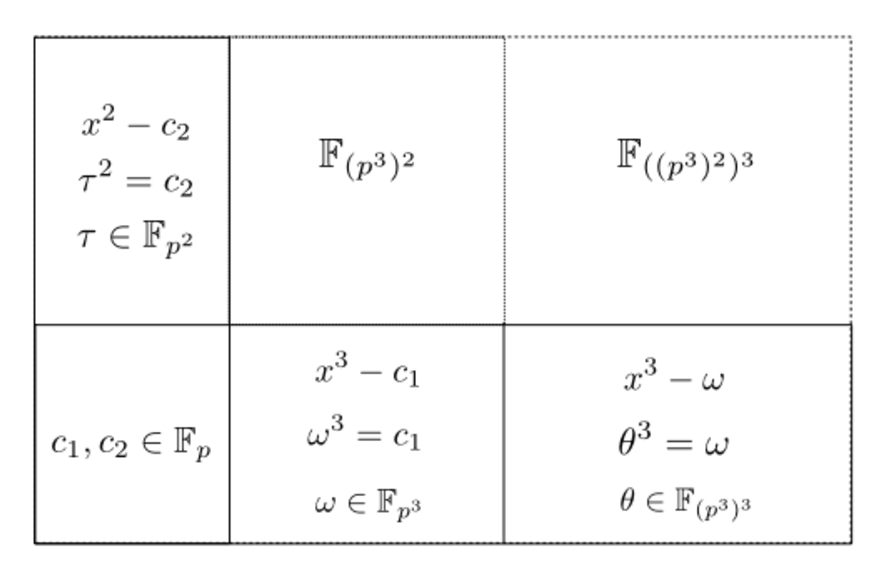
\includegraphics[width=7.5cm, height=4cm]{Field.eps}
\caption{Construction overview of $\FQTHTWTH$}
\label{fig_field}
\end{figure*}

\subsection{Arithmetic operations over extension field $\FQTH$}
At first, let us consider arithmetic operations in $\FQTH$, which is the degree $3$ extension field over $\FQ$. 
In order to perform arithmetic operations in $\FQTH$, we generally need an irreducible polynomial $f(x)$ of degree $3$ over $\FQ$. Specifically irreducible binomial is efficient to use as reduction modular polynomial. In order to obtain such binomial, Legendre symbol $\Leg{c_1}{p}$ is convenient.
Let us consider $3|(p-1)$ and a non-zero element $c_1 \in \FQ$. 
\begin{equation}\label{eq:legndre_3}
c_1^{\frac{p-1}{3}} = 
\begin{cases}
  0 \quad & \mbox{$c_1 = 0$},\\
  1 \quad &\mbox{CPR},\\
  otherwise & \mbox{CPNR},
\end{cases}
\end{equation}
where CPR and CPNR are abbreviations of cubic power residue and cubic power non residue, respectively. If $c_1$ does not have any cubic root in $\FQ$, $f(x) =x^3 - c_1$ becomes an irreducible binomial over $\FQ$. Let $\omega$ be a zero of $f(x)$, which is an element in $\FQTH$. Therefore the set $\left\lbrace 1, \omega, \omega^2 \right\rbrace $ forms a polynomial basis of $\FQTH$ over $\FQ$. Now let us consider two arbitrary element $\textbf{a, b}$ in $\FQTH$, can be represented as follows:
\begin{eqnarray}\label{eq:vec_A_Fq_3}
\textbf{a} & = & a_0 + a_1\omega+ a_2\omega^2,  \nonumber \\ 
\textbf{b} & = & b_0 + b_1\omega+ b_2\omega^2,  \nonumber \\
& & a_i, b_j \in \FQ .  \nonumber
\end{eqnarray} 

\subsubsection{Addition and subtraction in $\FQTH$}
Addition, subtraction within the elements and multiplication by a scalar with any element in $\FQTH$ are carried out by coefficient wise operations over $\f{p}$ as follows,
\begin{eqnarray}\label{eq:add_sub_fq3}
\textbf{a} \pm \textbf{b} & = &  (a_0 \pm b_0, a_1 \pm b_1, a_2 \pm b_2), \\
k\textbf{a} & = &  (ka_0,  ka_1,ka_2),  \mbox{ $k \in \FQ$}.
\end{eqnarray}

\subsubsection{Multiplication in $\FQTH$}
Multiplication of two arbitrary vectors is performed as follows:
%\begin{subequations}
\begin{eqnarray}
\textbf{ab} & = & (a_0 + a_1\omega+ a_2\omega^2)(b_0 + b_1\omega+ b_2\omega^2)\nonumber\\
& = & a_0 b_0 + (a_0 b_1+a_1 b_0)\omega + (a_0 b_2 +a_1 b_1 + a_2 b_0)\omega^2 \nonumber \\ 
&  & + (a_1 b_2+a_2 b_1)\omega^3 +a_2b_2\omega^4.  \label{eq:mul_fq3_a}
%& = &(a_0 b_0 + c_1 a_1 b_2 + c_1 a_2 b_1) + (a_0 b_1+ a_1 b_0 \nonumber \\
%& & + c_1 a_2 b_2)\omega + (a_0 b_2 +a_1 b_1 + a_2 b_0)\omega^2 \label{eq:mul_fq3_b}
\end{eqnarray}
%\end{subequations}
Here in \eqref{eq:mul_fq3_a}, there are 9 multiplications and 4 additions in $\FQ$. To reduce the number of multiplications in \eqref{eq:mul_fq3_a}, we apply Fast Polynomial Multiplication introduced in \cite{OEF} as follows:
\begin{eqnarray}\label{eq:FPM}
A_0 & = & a_0b_0\nonumber \\
A_1 & = & a_1b_1\nonumber \\
A_2 & = & a_2b_2\nonumber \\
A_3 & = & (a_0+ a_1)(b_0+b_1)\nonumber \\
A_4 & = & (a_0+ a_2)(b_0+b_2)\nonumber \\
A_5 & = & (a_1+ a_2)(b_1+b_2), 
\end{eqnarray}
where $A_i, i= 0,1, \cdots, 5$ are the auxiliary products. Let us consider $\textbf{ab} = t(\omega) = \sum_{i=0}^{4} t_i\omega^i$.
Now we can represent the coefficients $t(\omega)$ as only additions and subtractions of  $A_i$,
\begin{eqnarray}\label{eq:FPM1}
t_0 & = & A_0\nonumber \\
t_1 & = & A_3 - A_1 - A_0 \nonumber \\
& = & (a_0b_0 +a_0b_1+a_1b_0+a_1b_1)-a_1b_1-a_0b_0 \nonumber \\
t_2 & = & A_4 - A_2 - A_0 + A_1\nonumber \\
& = & (a_0b_0 +a_2b_0+a_0b_2+a_2b_2)-a_2b_2-a_0b_0 +a_1b_1\nonumber \\
t_3 & = & A_5 - A_1 - A_2\nonumber \\
& = & (a_1b_1 +a_1b_2+a_2b_1+a_2b_2)-a_1b_1-a_2b_2 \nonumber \\
t_4 & = & A_2.
\end{eqnarray}
Considering subtractions as additions, from the above equations we find that only 6 multiplications and 13 additions are required in $\FQ$ for multiplying two arbitrary vectors in $\FQTH$. Therefore, compared to \eqref{eq:mul_fq3_a} the above method will accelerate the vector multiplication, since in most processors multiplication is slower than addition. Substituting $\omega^3 = c_1$ in \eqref{eq:mul_fq3_a}, owing to the fact that $f(\omega) = 0$ of the irreducible binomial $f(x)=x^3-c_1$; $\textbf{ab}$ becomes as follows:
\begin{eqnarray}\label{fq_3_t}
\textbf{ab} & = & t_0 + t_1\omega + t_2\omega^2 + t_3 \omega^3 + t_4\omega^4 \nonumber \\
& = & (t_0 + c_1 t_3 ) + (t_1+c_1 t_4)\omega + t_2\omega^2.
\end{eqnarray}
Here it requires 2 more $\FQ$ additions. Multiplication with  $c_1$  will not increase the number of multiplications in $\FQ$ since $c_1$ is small such as $2$ and it can be achieved using bit wise shifting. Finally 6 multiplications and 15 additions are required in $\FQ$ to multiply two elements in $\FQTH$.

\subsubsection{Squaring in $\FQTH$}
Squaring of an $\FQTH$  element $A$ is performed by applying Chung-Hasan method \cite{chung2007asymmetric} as following.

\begin{eqnarray}\label{chung_h}
A^2 & = & (a_0 + a_1\omega + a_2\omega^2)^2 \nonumber\\
& =  & a_0^2 +2c_1a_1a_2 +[2a_0a_1 +c_1a_2^2]\omega+[(a_0 +a_1 +a_2)^2 \nonumber \\
&&-(a_0^2 + a_2^2 + 2a_1a_2 + 2a_0a_1)]\omega^2.
\end{eqnarray}
In what follows, let us consider \eqref{chung_h} be written as $\textbf{AB} = S_1 +S_2\omega + S_3\omega^2$ and  the coefficients are expressed as \eqref{sq_sub}. The following terms can be pre-calculated to reduce the number of operations. $ T_1= 2a_1$, $T_2 = a_0^2$, $T_3=a_2^2$, $T_4=T_1a_2$, $T_5=T_1a_0$, $T_6 = (a_0+a_1+a_2)^2$.
\begin{subequations} \label{sq_sub}
\begin{eqnarray}
S_1 & = & T_2+c_1T_4, \\
S_2 & = & T_5+c_1T_3,\\
S_3 & = & T_6 - (T_2+T_3+T4+T_5).
\end{eqnarray}
\end{subequations}
When $c_1 = 2$ , the operation cost of a squaring in $\FQTH$ is 2 multiplications, 3 squaring and 8 additions in $\FQ$ and 2 bit wise left shifting.
\subsubsection{Vector inversion in $\FQTH$}
The inverse element $\textbf{a}^{-1} \in \F{p}{3}$, can be easily calculated using Frobenius mapping (FM) $\pi(\textbf{a})$. At first we find the conjugates $\textbf{a}^p$, $\textbf{a}^{p^2}$ of $\textbf{a}$ by applying FM. Then the inverse element $\textbf{a}^{-1}$  is calculated as follows.
\begin{equation}
\textbf{a}^{-1} = n(\textbf{a})^{-1}(\textbf{a}^p\textbf{a}^{p^2}), \label{Inv_Cal_fq3}
\end{equation}
where $n(\textbf{a})= (\textbf{a}\textbf{a}^{p}\textbf{a}^{p^2}) \in \mFp$ is the product of conjugates. Conjugate $\textbf{a}^p=  (a_0+a_1\omega+a_2 \omega^2)^p$ can be easily calculated as follows:
\begin{eqnarray}\label{eq:FM_aq}
(a_0+a_1\omega+a_2 \omega^2)^p& = & (a_0 + a_1 \omega)^p+ (a_2 \omega^2)^p\nonumber\\
& = & a_0+a_1(\omega^3)^{\frac{p-1}{3}}\omega  \nonumber \\ 
& & + a_2 ((\omega^3)^{\frac{p-1}{3}})^2 \omega^2  \nonumber \\ 
& = & a_0+a_1(c_1)^{\frac{p-1}{3}} \omega  \nonumber \\
& & + a_2 ((c_1)^{\frac{p-1}{3}})^2 \omega^2 \nonumber \\
& = & a_0 + a_1 c_1' \omega + a_2 c_1'' \omega^2 \nonumber \\
& = & a_0 + a_1' \omega + a_2' \omega^2,
\end{eqnarray}
where $a_1', a_2' \in \FQ$ and $c_1' = (c_1)^{\frac{p-1}{3}}$ is already known from \eqref{eq:legndre_3} and $c_1'' = (c_1')^2$ can be precalculated. In the above computation, 2 multiplications in $\FQ$ is required. 
Now the other conjugate $\textbf{a}^{p^2}$ can be calculated with the same number of operations according to the above procedure as follows:
\begin{eqnarray}
\textbf{a}^{p^2} & = & (\textbf{a}^p)^p\nonumber \\
& = &  (a_0 + a_1' \omega + a_2' \omega^2)^p\nonumber \\
& = & a_0 + a_1' c_1' \omega + a_2' c_1'' \omega^2 \nonumber \\
& = & a_0 + a_1'' \omega + a_2'' \omega^2,
\end{eqnarray} 
where $a_1'', a_2'' \in \FQ$.
Before calculating $n(\textbf{a})$ we first calculate the multiplication of $(\textbf{a}^p\textbf{a}^{p^2})$ like \eqref{eq:mul_fq3_a} as follows
\begin{eqnarray}\label{eq:mul_aq_aq2}
\textbf{a}^p\textbf{a}^{p^2} & = & (a_0 + a_1'\omega+ a_2'\omega^2)(a_0 + a_1''\omega+ a_2''\omega^2).
%& = & (a_0^2 + c_1a_1' a_2''+c_1a_2' a_1'') + (a_0 a_1' + a_0 a_1'' \nonumber \\
%& & +c_1a_2'a_2'')\omega + (a_0 a_2' +a_1' a_1'' + a_0 a_2'')\omega^2.
\end{eqnarray}
Now let us consider the following representation. \\ $\textbf{T}= \textbf{a}^p\textbf{a}^{p^2}  = (t_0,t_1,t_2), \quad  n(\textbf{a}) =s= \textbf{aT}$,\\
Thereby the inversion of $\textbf{a}$ can be expressed as $\textbf{a}^{-1}= s^{-1}\textbf{T}$.
The vector representation of the non-zero scalar $s$ is written as $s = (s,0,0)$. 
In addition, $\textbf{a}^p$ and $\textbf{a}^{p^2}$ is represented by the following equations by using the relation $c_1'^2+c_1'+1=0$, where $c_1'^3=1$.
\begin{subequations}
\begin{equation}
\textbf{a}^p  =  (a_0, c_1' a_1, c_1'^2 a_2)  =  (a_0, c_1'a_1,-a_2-c_1'a_2),
\end{equation}
\begin{equation}
\textbf{a}^{p^2} =  (a_0, c_1'^2 a_1, c_1' a_2)  =  (a_0, -a_1-c_1'a_1,c_1'a_2).
\end{equation}
\end{subequations}
Now let us consider the variables $T_0 \sim T_5$ as following expressions.
\begin{subequations}
\begin{eqnarray}
 T_0 & = & a_0^2,\nonumber \\
  T_1 & = & a_1^2, \nonumber \\
  T_2 & = & a_2^2, \nonumber \\
 T_3 & = & (c_1'a_1+c_1'^2a_2)(c_1'^2a_1+c_1'a_2)\nonumber \\
 &  = & a_1^2-a_1a_2+a_2^2\nonumber\\
 T_4 & = & (a_0+c_1'a_1)(a_0+c_1'^2a_1)\nonumber\\
 &= &a_0^2-a_0a_1+a_1^2\nonumber\\
 T_5 & = & (a_0+c_1'^2a_2)(a_0+c_1'a_2)\nonumber\\
 &= & a_0^2-a_0a_2+a_2^2.\nonumber
 \end{eqnarray}
\end{subequations}
The elements of $\textbf{T} = (t_0,t_1,t_2)$ can be obtained as follows:
\begin{subequations}
\begin{eqnarray}
t_1  & = &   T_0 + c_1 (T_3 - T_1 - T_2) \nonumber \\
& = & a_0^2 - c_1a_1a_2,\\
t_2 & = & T_4- T_0 - T_1 +c_1 T_2 \nonumber\\
& = & c_1a_2^2 - a_0a_1,\\
t_3 & = & T_5 -T_0 - T_2 +T_1 \nonumber \\
& = & a_1^2 - a_0a_2.
\end{eqnarray}
\end{subequations}
The calculation cost of $t_1,t_2,t_3$ is 3 multiplications, 3 squaring, 3 additions and 2 bit shifting. The vector multiplication for getting $s = \textbf{aT} =(s,0,0)$ can be done by calculating $s = a_0b_0+c_1(a_1b_2+a_2b_1)$ which costs 3 multiplication, 2 additions and 1 bit shifting. 

Finally the inversion of the scalar $s$ and multiplication by the inverse of scalar $s$ with vector $\textbf{T}= \textbf{a}^p\textbf{a}^{p^2}$ can be obtained by distributive law which takes 1 inversion and 3 multiplication in $\FQ$. Therefore the total cost of inversion is 9 multiplications, 3 squaring, 5 additions, 3 bit shifting and 1 inversion in $\Fp$. 

%This result can be saved for further use. Thus \eqref{eq:mul_aq_aq2} has 6 multiplications and 15 additions in $\FQ$ according to \eqref{eq:FPM} and \eqref{eq:FPM1}. Similarly multiplying $\textbf{a}$ with \eqref{eq:mul_aq_aq2} yields $n(\textbf{a})$ which will have no $\omega$ terms. That is $n(\textbf{a})$  will be a scalar. The total calculation cost for $n(\textbf{a})$ is 16 multiplications and 26 additions. Therefore the inversion of $\textbf{a} \in \FQTH$ can be easily calculated from \eqref{Inv_Cal_fq3} with 19 multiplications, 26 additions and 1 inversion in $\FQ$. 

\subsection{Arithmetic operations over extension field $\FQTHTW$}
$\FQTHTW$ is constructed with the irreducible binomial $g(x)=x^2-c_2$ where $c_2 \in \FQ$. Here it differs from the existing method to towering. Existing method uses $x^2-\omega$ as the irreducible polynomial in $\FQSX$; that is the root of irreducible binomial of $\FQTH$ is used to construct irreducible binomial in $\FQSX$. In this proposed approach, such binomial can be easily obtained by applying Legendre Symbol $\Leg{c_2}{p}$ over $\FQ$. Then let its zero be $\tau$,$\tau \in \FQTHTW$, therefore the set $\left\lbrace 1, \tau \right\rbrace $ forms the polynomial basis in $\FQTHTW$. If we choose $p$ such that $p \equiv 3$ (mod $4$), that will accelerate the arithmetic operation significantly; since multiplication by $c_2=-1$ will be calculated only by substitution. Let us consider $\textbf{m},\textbf{n}$ as two arbitrary elements in $\FQTHTW$ as follows:

\begin{eqnarray}\label{eq:vec_mn_Fp3_2}
\textbf{m} & = & \textbf{a}_0 + \textbf{a}_1\tau,  \nonumber \\ 
\textbf{n} & = & \textbf{b}_0+\textbf{b}_1 \tau,  \nonumber \\
& & \textbf{a}_i, \textbf{b}_j \in \F{p}{3}.  \nonumber
\end{eqnarray} 

Addition and Subtraction is done coefficient wise similar to those in $\FQTH$. Multiplication of $\textbf{m},\textbf{n}$ is done as follows:
\begin{eqnarray}\label{eq:mul__Fp_3_2}
\textbf{mn} & = & (\textbf{a}_0+\textbf{a}_1\tau)(\textbf{b}_0+\textbf{b}_1\tau)\nonumber\\
& = & \textbf{a}_0 \textbf{b}_0 + (\textbf{a}_0 \textbf{b}_1+\textbf{a}_1 \textbf{b}_0)\tau + \textbf{a}_1\textbf{b}_1\tau^2 \nonumber \\ 
& = &(\textbf{a}_0 \textbf{b}_0 + c_2 \textbf{a}_1 \textbf{b}_1)+ (\textbf{a}_0 \textbf{b}_1+\textbf{a}_1 \textbf{b}_0)\tau  \label{eq:mul_Fp_3_2a}\\ 
& = &(\textbf{a}_0 \textbf{b}_0 + c_2 \textbf{a}_1 \textbf{b}_1) + (\textbf{a}_0 +\textbf{a}_1)( \textbf{b}_0 +\textbf{b}_1)\tau \nonumber \\ 
&    &  - (\textbf{a}_0\textbf{b}_0)\tau - (\textbf{a}_1\textbf{b}_1)\tau.
\end{eqnarray}
Here Karatsuba method \cite{Karatsuba} is applied. In this calculation, we have substituted $\tau^2 = c_2$, as $\tau$ is a zero of the irreducible binomial $g(x)=x^2-c_2$. Since prime number $p$ is chosen such that $p \equiv 3$ (mod $4$), therefore $c_2$  is just substituted with $-1$. That means  multiplication with $c_2$ needs no countable computations in $\FQ$. Moreover multiplication of $\textbf{a}_1\textbf{b}_1$ and $\textbf{a}_0\textbf{b}_0$ will be reused. Therefore we need 3 multiplications and 5 additions in $\FQTH$ to multiply two vectors over $\FQTHTW$, where we consider subtractions as additions.

\subsubsection{Vector inversion in $\FQTHTW$}
For calculating the multiplicative inverse vector of a non-zero vector $\textbf{m}\in \FQTHTW$, first we calculate the conjugate of $\textbf{m}$ that is given by  Frobenius mapping  $\pi_{p^3}(\textbf{m}) = \textbf{m}^{p^3}$. Then the inverse of $\textbf{m}$, $\textbf{m}^{-1}$ is calculated as follows:
\begin{equation}\label{InvCal_fq_3_2}
\textbf{m}^{-1} = n(\textbf{m})^{-1}(\textbf{m}^{p^3}), 
\end{equation}
where  $\textbf{m}$, $\textbf{m}^{p^3}$ are the conjugates and $n(\textbf{m})$ is their product. FM of $\textbf{m}$, $\pi_{p^3}(\textbf{m}) =  (\textbf{a}_0+\textbf{a}_1\tau)^{p^3}$ can be easily calculated using the defined irreducible binomial $g(x)$ as follows:
\begin{eqnarray}\label{eq:FM_fq_3_2}
(\textbf{a}_0+\textbf{a}_1\tau)^{p^3} & = & \textbf{a}_0+\textbf{a}_1\tau^{p^3} \nonumber \\
& = & \textbf{a}_0+\textbf{a}_1(\tau^2)^{\frac{p^3-1}{2}}\tau \nonumber \\ 
& = & \textbf{a}_0+\textbf{a}_1(c_2)^{\frac{p^3-1}{2}}\tau \nonumber \\
& = & \textbf{a}_0-\textbf{a}_1\tau,
\end{eqnarray}
where the modular relation $\tau^2 = c_2 $ and $c_2 = -1$ is substituted. In other words, the conjugate of $\textbf{m}$ is given as $\textbf{a}_0-\textbf{a}_1\tau$. No addition and multiplication is required here. Now the calculation procedure for $n(\textbf{m}) = \textbf{m}\textbf{m}^{p^3}$ is as follows:
\begin{eqnarray}\label{eq:Inversion}
n(\textbf{m}) & = & (\textbf{a}_0+\textbf{a}_1\tau)(\textbf{a}_0 -\textbf{a}_1\tau)\nonumber\\
& = & \textbf{a}_0^2 - \textbf{a}_1^2\tau^2 \nonumber \\ 
& = & \textbf{a}_0^2 - c_2\textbf{a}_1^2 \nonumber \\ 
& = & \textbf{a}_0^2 + \textbf{a}_1^2.
\end{eqnarray}
Here 2 squaring and 1 addition is required over $\FQTH$. Since $n(\textbf{m})$ is given without $\tau$, it is found that $n(\textbf{m}) \in \F{p}{3}$. Therefore, the inversion element  $n(\textbf{m})^{-1}$ is calculated using \eqref{Inv_Cal_fq3}  over $\FQTH$. Finally 2 multiplications, 2 squaring, 1 inversion and 1 addition in $\FQTH$ is required to get an inverse element over $\FQTHTW$.

\subsection{Arithmetic operations over extension field $\FQTHTWTH$}
To construct $\FQTHTWTH$ arithmetic operation let us consider irreducible binomial $h(x)=x^3-\omega$ where $\omega \in \F{p}{3}$ and $\omega$ is the root of $f(x)$. Then let $\theta$ be a root of $h(x)$, where $\theta \in \FQTHTWTH$, therefore the set $\left\lbrace 1, \theta, \theta^2 \right\rbrace$ forms the polynomial basis in $\FQTHTWTH$. Let us consider $\textbf{u},\textbf{v}$ as two arbitrary elements in $\FQTHTWTH$ as follows:
\begin{eqnarray}\label{eq:vec_uv_Fp_3_2_3}
\textbf{u} & = & \textbf{m}_0 + \textbf{m}_1\theta + \textbf{m}_2\theta^2,  \nonumber \\ 
\textbf{v} & = & \textbf{n}_0 + \textbf{n}_1\theta+ \textbf{n}_2\theta^2,  \nonumber \\
& &  \textbf{m}_i,  \textbf{n}_j \in  \FQTHTW. \nonumber
\end{eqnarray} 
In  $\FQTHTWTH$, vector addition and subtraction is performed coefficient wise over  $\FQTHTW$. 
Multiplication of  $\textbf{u},\textbf{v}$ is performed by using $h(x)$ as follows:
\begin{eqnarray}\label{eq:mul_fq_3_2_3}
\textbf{uv} & = & (\textbf{m}_0 + \textbf{m}_1\theta + \textbf{m}_2\theta^2)( \textbf{n}_0 + \textbf{n}_1\theta+ \textbf{n}_2\theta^2).
%& = & \textbf{m}_0 \textbf{n}_0 + (\textbf{m}_0 \textbf{n}_1+\textbf{m}_1 \textbf{n}_0)\theta  \nonumber \\ 
%&  & + (\textbf{m}_0 \textbf{n}_2 +\textbf{m}_1 \textbf{n}_1 + \textbf{m}_2 \textbf{n}_0)\theta^2 \nonumber \\ 
%&  & + (\textbf{m}_1 \textbf{n}_2+\textbf{m}_2 \textbf{n}_1)\theta^3 +\textbf{m}_2\textbf{n}_2\theta^4.
%& = &(\textbf{m}_0 \textbf{n}_0 + \omega \textbf{m}_1 \textbf{n}_2 + \omega \textbf{m}_2 \textbf{n}_1)  \nonumber \\
%& & + (\textbf{m}_0 \textbf{n}_1+ \textbf{m}_1 \textbf{n}_0 + \omega \textbf{m}_2 \textbf{n}_2)\theta \nonumber \\
%& & + (\textbf{m}_0 \textbf{n}_2 +\textbf{m}_1 \textbf{n}_1 + \textbf{m}_2 \textbf{n}_0)\theta^2.
\end{eqnarray}
 After applying fast polynomial multiplication according to \eqref{eq:FPM} and \eqref{eq:FPM1}, here we have 6 multiplications and 15 additions in $\FQTHTW$ as follows:
\begin{eqnarray}\label{mul_3_2_3}
\textbf{uv} & = & t_0' + t_1'\theta + t_2'\theta^2 + t_3' \theta^3 + t_4'\theta^4 \nonumber \\
& = & (t_0 + \omega t_3 ) + (t_1+\omega t_4)\theta + t_2'\theta^2.
\end{eqnarray}

%To calculate  $\omega \textbf{m}_i \textbf{n}_j$ terms first we perform multiplication between $\textbf{m}_i \textbf{n}_j$ in $\FQTHTW$ according to \eqref{eq:mul_Fp_3_2a}. After that $\omega$ is multiplied to each coefficient of the resulted vector as follows:
%\begin{eqnarray}\label{eq:mul_omega_3_2}
%\omega \textbf{mn} & = &\omega (\textbf{a}_0 \textbf{b}_0 + c_2 \textbf{a}_1 \textbf{b}_1) + \omega (\textbf{a}_0 +\textbf{a}_1)( \textbf{b}_0 +\textbf{b}_1)\tau \nonumber \\ 
%&    &  - \omega(\textbf{a}_0\textbf{b}_0)\tau - \omega(\textbf{a}_1\textbf{b}_1)\tau.
%\end{eqnarray}
Multiplication of basis element with vector will not effect the calculation since it is comparatively small, which will be calculated as bit wise shifting.

\subsubsection{Vector inversion in $\FQTHTWTH$}
Inversion of $\FQTHTWTH$ vector can be easily carried out by applying the similar steps of $\FQTH$ vector inversion. 
For calculating the multiplicative inverse vector of a non-zero vector $\textbf{v}\in \FQTHTWTH$, at first we find the conjugates $\textbf{v}^{p^6}$, $\textbf{v}^{p^{12}}$ of $\textbf{v}$ applying FM. Then the inverse element $\textbf{v}^{-1}$  is calculated as follows:
\begin{equation}
\textbf{v}^{-1} = n(\textbf{v})^{-1}(\textbf{v}^{p^6}\textbf{v}^{p^{12}}), \label{InvCal_fq_3_2_3}
\end{equation}
where  $\textbf{v}$, $\textbf{v}^{p^6},\textbf{v}^{p^{12}}$ are the conjugates and $n(\textbf{v})$ is their product. Here we first calculate $\pi_{p^6}(\textbf{v})  =  (\textbf{n}_0+\textbf{n}_1\theta + \textbf{n}_2 \theta^2)^{p^6}$ using the defined irreducible binomial $h(x)$ as follows:
\begin{eqnarray}\label{eq:FM_fq_3_2_3}
(\textbf{n}_0+\textbf{n}_1\theta+\textbf{n}_2 \theta^2)^{p^6} & = & (\textbf{n}_0 + \textbf{n}_1 \theta)^{p^6}+ (\textbf{n}_2 \theta^2)^{p^6} \nonumber\\
& = & \textbf{n}_0+\textbf{n}_1(\theta^3)^{\frac{p^6-1}{3}}\theta  \nonumber \\ 
& & + \textbf{n}_2 ((\theta^3)^{\frac{p^6-1}{3}})^2 \theta^2  \nonumber \\ 
& = & \textbf{n}_0+\textbf{n}_1(\omega)^{\frac{p^6-1}{3}} \theta  \nonumber \\
& & + \textbf{n}_2 ((\omega)^{\frac{p^6-1}{3}})^2 \theta^2 \nonumber \\
& = & \textbf{n}_0+\textbf{n}_1(\omega^3)^{\frac{p^6-1}{9}} \theta  \nonumber \\
& & + \textbf{n}_2 ((\omega^3)^{\frac{p^6-1}{9}})^2 \theta^2 \nonumber \\
& = & \textbf{n}_0+\textbf{n}_1(c_1)^{\frac{p^6-1}{9}} \theta  \nonumber \\
& & + \textbf{n}_2 ((c_1)^{\frac{p^6-1}{9}})^2 \theta^2 \nonumber \\
& = & \textbf{n}_0 + \textbf{n}_1 c_{\omega}' \theta + \textbf{n}_2 c_{\omega}'' \theta^2 \nonumber \\
& = & \textbf{n}_0 + \textbf{n}_1' \theta + \textbf{n}_2' \theta^2 ,
\end{eqnarray}
%Here we have 2 multiplication in $\FQTHTW$ and 1 squaring in $\FQTH$.

where $n_1', n_2' \in \FQTHTW$ and $c_{\omega}' = (c_1)^{\frac{p^6-1}{9}}$, $c_{\omega}'' = (c_{\omega}')^2$ can be precalculated. Therefore only 6 multiplications in $\FQ$ is required in the above calculation. 
Now the other conjugate  $\textbf{v}^{p^{12}}$ can be calculated according to the above procedure with the same number of operations as follows: 
\begin{eqnarray}\label{fm_fq_12}
\textbf{v}^{(p^6)^2} & = & (\textbf{v}^{p^{12}}) \nonumber \\
& = &  (\textbf{n}_0 + \textbf{n}_1' \theta + \textbf{n}_2' \theta^2)^{p^{6}} \nonumber \\
& = & \textbf{n}_0 + \textbf{n}_1' c_{\omega}' \theta + \textbf{n}_2' c_{\omega}'' \theta^2 \nonumber \\
& = & \textbf{n}_0 + \textbf{n}_1'' \theta + \textbf{n}_2'' \theta^2 .
\end{eqnarray} 
%Above result will be multiplied with $\textbf{v}$ to calculate $n(\textbf{v})$, where $n(\textbf{v}) \in \FQTH$. Therefore  $n(\textbf{v})^{-1}$ will be calculated according to  \eqref{Inv_Cal_fq3} in $\FQTH$. 
Now computation of $(\textbf{v}^{p^6}\textbf{v}^{p^{12}})$ according to \eqref{mul_3_2_3} will cost 6 multiplication and 15 additions in $\FQTHTW$ as follows: 
\begin{eqnarray}\label{eq:mul_v6_v12}
\textbf{v}^{p^6}\textbf{v}^{p^{12}} & = & (\textbf{n}_0 + \textbf{n}_1' \theta + \textbf{n}_2' \theta^2)(\textbf{n}_0 + \textbf{n}_1'' \theta + \textbf{n}_2'' \theta^2).
%& = & (a_0^2 + c_1a_1' a_2''+c_1a_2' a_1'') + (a_0 a_1' + a_0 a_1'' \nonumber \\
%& & +c_1a_2'a_2'')\omega + (a_0 a_2' +a_1' a_1'' + a_0 a_2'')\omega^2.
\end{eqnarray}
The next calculation procedure is identical of $\FQTH$ vector inversion which also results the same number of operation counts in $\FQSX$.
Finally the total cost of 1 vector inversion in $\FQEN$ is 9 multiplications, 3 squaring, 5 additions, 3 bit shifting and 1 inversion in $\FQSX$. 

%Similarly $\textbf{v}$ is multiplied to \eqref{eq:mul_v6_v12} to calculate $n(\textbf{v})$. It costs same number of operations as \eqref{eq:mul_v6_v12}. Since  $n(\textbf{v}) \in \FQSX$, therefore  $n(\textbf{v})^{-1}$ will be calculated according to  \eqref{InvCal_fq_3_2} in $\FQSX$. Finally we need 12 multiplications, 30 additions and 1 inversion in $\FQTHTW$; 12 multiplications in $\FQ$ to calculate an inverse element in $\FQTHTWTH$.

%Similarly $\textbf{v}$ is multiplied to \eqref{eq:mul_v6_v12} to calculate $n(\textbf{v})$. It costs same number of operations as \eqref{eq:mul_v6_v12}. Since  $n(\textbf{v}) \in \FQTH$, therefore  $n(\textbf{v})^{-1}$ will be calculated according to  \eqref{Inv_Cal_fq3} in $\FQTH$. Finally we need 12 multiplications, 26 additions in $\FQTHTW$; 1 inversion, 6 multiplications in $\FQTH$ and 12 multiplications in $\FQ$ to calculate an inverse element in $\FQTHTWTH$.

\section{Result evaluation}
The main focus of this proposal is to show the construction procedure of $\FQEN$ extension field in a new approach of towering that will lead to efficient arithmetic operation. We can also apply sub-field isomorphic group arithmetic or Cyclic Vector Multiplication Algorithm (CVMA) to reduce the number of additions and multiplication in each extension field which will make this towering construction more efficient. But that is not focused in this paper.

Table \ref{tab11} shows the environment, used to experiment and evaluate the proposed method.  
\renewcommand{\baselinestretch}{1.5}
\begin{table}[!ht]
\renewcommand{\arraystretch}{1.3}
\centering
\caption{ Computational Environment}
\label{tab11}
\begin{tabular}{|c|c|}
\hline 
• & PC \\ 
\hline \hline 
CPU {\textsuperscript{*}} & \quad 2.7 GHz Intel Core i5 \quad \\ 
\hline 
Memory & 16 GB \\ 
\hline 
OS & Mac OS X 10.11.4  \\ 
\hline 
Compiler & gcc 4.2.1 \\ 
\hline 
\quad Programming Language \quad  & C \\ 
\hline 
Library & GNU MP\\ 
\hline 
\multicolumn{2}{l}{\textsuperscript{*}\footnotesize{Only single core is used from two cores.}}\\
\end{tabular} 
\end{table}
\renewcommand{\baselinestretch}{1.0}

In the experiment we have used  Kachisa-Schaefer-Scott (KSS) \cite{kss} pairing friendly curves with embedding degree $k = 18$ at the 192-bit security level. The prime number $p = 511$-bit is considered and the curve is defined as $y^2=x^3+11$.

In what follows, let us consider $m,s,a$ and $i$ to denote the times of multiplication, squaring, addition and inversion respectively. The bit wise shifting operation is not taken into account during the final operation count.
Table \ref{tab1} shows the calculation cost in the context of  operation count and Table \ref{tab3} shows the execution time.
\renewcommand{\baselinestretch}{1.5}
\begin{table}[!ht]
\renewcommand{\arraystretch}{1.3}
\centering
\caption{$\FQTHTWTH$ operation count}
\label{tab1}
\resizebox{\columnwidth}{!}{
\begin{tabular}{c||c|c}
\hline 
 Operation in & 1 inversion in $\FQEN$ & 1 multiplication in $\FQEN$\\ 
\hline\hline 
%$\FQSX$ & $9m+3s+5a+1i$ &  $9m+3s+5a+1i$ \\ \hline 
%$\FQTH$ & $9m+3s+5a+1i$ &  $9m+3s+5a+1i$ \\ \hline 
$\FQ$ & $199m+9s+660a+1i$ &  $108m+402a$ \\ 
\hline 
\end{tabular} 
}
\end{table}

%\begin{table}[!ht]
%\renewcommand{\arraystretch}{1.3}
%\centering
%\caption{Number of multiplication and addition for multiplication of two elements in $\FQTHTWTH$}
%\label{tab2}
%\begin{tabular}{c||c|c}
%\hline 
%Extension Field Type & \#MUL in $\FQ$ & \#ADD in ${\FQ}$\\ 
%\hline\hline 
%$\FQTHTWTH$ & 108 & 402 \\
%\hline 
%\end{tabular}
%\end{table}

\begin{table}[!ht]
\renewcommand{\arraystretch}{1.3}
\centering
\caption{Execution time [ms] for inversion and multiplication in $\FQTHTWTH$}
\label{tab3}
\begin{tabular}{c|c}
\hline 
Operation & Execution time[ms] \\ 
\hline\hline 
Inversion &  $5.4 \times  10^{-1}$ \\
\hline
Multiplication & $3.3 \times  10^{-1}$ \\
\hline  
\end{tabular}
\end{table}
\renewcommand{\baselinestretch}{1.0}
From Table \ref{tab1} we find that only 199 multiplication, 9 squaring, 660 additions and 1 inversion is required in $\Fp$ to perform 1 inversion in $\FQEN$.
There exist a competitive toweting scheme prsented by Aranha et al. \cite{aranha} that uses sub-field isomorphic group to reduce number of arithmetic operation. Such isomorphic sub-field isomorphic rational point group technique can also be applied in the proposed towering approach which will be presented as our future work.
\section{Conclusion and future work}
In this paper we have presented a new towering scheme to construct $\FQEN$ extension field arithmetic. This towering approach is one of the most important step for constructing the basis of pairing based cryptography defined over extension field of degree 18. This paper also presented the mathematical derivation for efficiently constructing the $\FQTHTWTH$ extension field to accelerate arithmetic operation in $\FQEN$. The main focus of this paper was to present the new towering technique along with its implementation procedure that can be used for performing operation efficiently in the context of pairing based cryptography. As our future work, we would like to reduce the number of arithmetic operation by applying sub-field isomorphic rational point group technique in the proposed towering approach along with some pairing algorithms implementation in practical case.
 %:  NO NEED s

Efficient Optimal Ate Pairing at 128-bit Security Level.

Following the emergence of Kim and Barbulescu's new number field sieve (exTNFS) algorithm at CRYPTO'16 \cite{kim_ecdlp} for solving discrete logarithm problem (DLP) over the finite field; pairing-based cryptography researchers are intrigued to find new parameters that confirm standard security levels against exTNFS. 
Recently, Barbulescu and Duquesne have suggested new parameters \cite{sylvain_new_param} for well-studied pairing-friendly curves i.e., Barreto-Naehrig (BN) \cite{BN}, Barreto-Lynn-Scott (BLS-12) \cite{ec_ex} and Kachisa-Schaefer-Scott (KSS-16) \cite{kss} curves at 128-bit security level (twist and sub-group attack secure). 
They have also concluded that in the context of Optimal-Ate pairing with their suggested parameters, BLS-12 and KSS-16 curves are more efficient choices than BN curves. 
Therefore, this paper selects the atypical and less studied pairing-friendly curve in literature, i.e., KSS-16 which offers quartic twist, while BN and BLS-12 curves have sextic twist.
In this paper, the authors optimize Miller's algorithm of Optimal-Ate pairing for the KSS-16 curve by deriving efficient sparse multiplication and implement them.
Furthermore, this paper concentrates on the Miller's algorithm to experimentally verify Barbulescu et al.'s estimation.
The result shows that Miller's algorithm time with the derived pseudo 8-sparse multiplication is most efficient for KSS-16 than other two curves.
Therefore, this paper defends Barbulescu and Duquesne's conclusion for 128-bit security.


\section{Introduction}
Since the inception by Sakai et al. \cite{sakai2000cryptosystems}, pairing-based cryptography has gained much attention to cryptographic researchers as well as  to mathematicians. It gives flexibility to protocol researcher to innovate applications with provable security and at the same time to mathematicians and cryptography engineers to find efficient algorithms to make pairing implementation more efficient and practical.
This paper tries to efficiently carry out the basic operation of a specific type of pairing calculation over certain pairing-friendly curves. 

Generally, a pairing is a bilinear map $e$ typically defined as  $\g1 \times \g2 \to \g3$, where $\g1$ and $\g2$ are additive cyclic sub-groups of  order $r$  on a certain elliptic curve $E$ over a finite extension field $\FPK$ and $\g3$ is a multiplicative cyclic group of order $r$ in $\mF{p}{k}$.
Let $E(\Fp)$ be the set of rational points over the prime field $\Fp$ which forms an additive Abelian group together with the point at infinity $\cal{O}$. The total number of rational points is denoted as $\#E(\Fp)$. Here, the order $r$ is a large prime number such that $r | \#E(\Fp)$ and gcd$(r,p)=1$. The embedding degree $k$ is the smallest positive integer such that $r | (p^k -1)$.
 Two basic properties of pairing are
 \begin{itemize}
 \item bilinearity is such that $\forall P_i \in \g1$ and $\forall Q_i \in \g2$, where $i= 1, 2$, then $e(Q_1+Q_2,P_1) = e(Q_1,P_1). e(Q_2,P_1)$ and $e(Q_1,P_1+P_2) = e(Q_1,P_1). e(Q_1,P_2)$,
 \item and $e$ is non-degenerate means $\forall P \in \g1$ there is a $Q \in \g2$ such that  $e(Q,P) \neq 1$ and $\forall Q \in \g2$ there is a $P \in \g1$ such that $e(P,Q) \neq 1$.
 \end{itemize}
Such properties allows researchers to come up with various cryptographic applications including ID-based encryption \cite{C:BonFra01}, group signature authentication \cite{group_sign_1}, and functional encryption \cite{okamoto2010fully}.  However, the security of pairing-based cryptosystems depends  on 
\begin{itemize}
\item  the difficulty of solving elliptic curve discrete logarithm problem (ECDLP) in the groups of order $r$ over $\Fp$,
\item  the infeasibility of solving the discrete logarithm problem (DLP) in the multiplicative group $\g3 \in \mF{p}{k}$,
\item and the difficulty of pairing inversion.
\end{itemize}
To maintain the same security level in both groups, the size of the order $r$ and extension field $p^k$ is chosen accordingly. If the desired security level is $\delta$ then $\log_2 r  \geq 2\delta$ is desirable due to Pollard's rho algorithm.  For efficient pairing, the ratio $\rho = \log_2 p^k/ \log_2 r \approx 1$,   is expected (usually  $1\leq  \rho  \leq 2$). In practice, elliptic curves with small embedding degrees $k$ and large $r$ are selected and commonly are knows as ``pairing-friendly" elliptic curves.

Galbraith et al. \cite{galbraith2008pairings} have classified pairings as three major categories based on the underlying group's structure as 
\begin{itemize}
\item Type 1, where $\g1 = \g2$, also known as symmetric pairing. 
\item Type 2, where $\g1 \neq \g2$, known as asymmetric pairing. There exists an efficiently computable isomorphism $\psi : \g2 \to \g1$ but none in reverse direction.
\item Type 3, which is also asymmetric pairing, i.e., $\g1 \neq \g2$. But no efficiently computable isomorphism is known in either direction  between $\g1$ and $\g2$.
\end{itemize}
This paper chooses one of the Type 3 variants of pairing named as Optimal-Ate \cite{op_ate_p} with Kachisa-Schaefer-Scott (KSS) \cite{kss} pairing-friendly curve of embedding degree $k=16$. 
Few previous works have been done on this  curve. 
Zhang et al. \cite{zhang_L12} have shown the computational estimation of the Miller's loop and proposed efficient final exponentiation for 192-bit security level in the context of Optimal-Ate pairing over KSS-16 curve. 
A few years later Ghammam et al. \cite{loubna_kss16} have shown that KSS-16 is the best suited for multi-pairing (i.e., the product and/or the quotient) when the number of pairing is more than two. 
Ghammam et al. \cite{loubna_kss16} also corrected the flaws of proposed final exponentiation algorithm by Zhang et al. \cite{zhang_L12} and proposed a new one and showed the vulnerability of Zhang's parameter settings against small subgroup attack. 
The recent development of NFS by Kim and Barbulescu \cite{kim_ecdlp} requires updating the parameter selection for all the existing pairings over the well known pairing-friendly curve families such as BN \cite{BN}, BLS \cite{EPRINT:FreScoTes06} and KSS \cite{kss}.
The most recent study by Barbulescu et al. \cite{sylvain_new_param} have shown the security estimation of the current parameter settings used in well-studied curves and proposed new parameters, resistant to small subgroup attack.

Barbulescu and Duquesne's study finds that the current parameter settings for 128-bit security level on BN-curve studied in literature can withstand for 100-bit security. 
Moreover, they proposed that BLS-12 and surprisingly KSS-16 are the most efficient choice for Optimal-Ate pairing at the 128-bit security level. Therefore, the authors focus on the efficient implementation of the less studied KSS-16 curve for Optimal-Ate pairing by applying the most recent parameters.
Mori et al. \cite{mori} and Khandaker et al. \cite{self_ICISC} have shown a specific type of sparse multiplication for BN and KSS-18 curve respectively where both of the curves supports sextic twist. 
The authors have extended the previous works for quartic twisted KSS-16 curve and derived pseudo-8 sparse multiplication for line evaluation step in the Miller's algorithm. 
As a consequence, the authors made the choice to concentrate on Miller's algorithm's execution time and computational complexity to verify the claim of \cite{sylvain_new_param}.
The implementation shows that Miller's algorithm time has a tiny difference between KSS-16 and BLS-12 curves. However, they both are more efficient and faster than BN curve. 



\section{Fundamentals of Elliptic Curve and Pairing}
\subsection{Kachisa-Schaefer-Scott (KSS) Curve}
In \cite{kss}, Kachisa, Schaefer, and Scott proposed a family of non super-singular pairing-friendly elliptic curves of embedding degree $k = \left\lbrace16, 18, 32, 36, 40\right\rbrace$, using elements in the cyclotomic field. 
 In what follows, this paper considers  the curve of embedding degree $k =16$, named as \textit{KSS-16}, defined over extension field $\FPSN$ as follows:
\begin{equation}\label{eq:KSS_16}
E/\FPSN:Y^2=X^3+aX, \quad \mbox{($a \in \Fp$) and  $a \neq 0$},
\end{equation}
 where $X,Y \in \FPSN$. Similar to other pairing-friendly curves,  \textit{characteristic} $p$, \textit{Frobenius trace} $t$ and \textit{order} $r$ of this curve are given by the following polynomials of  integer variable $u$.
\begin{subequations}
\begin{eqnarray}
p(u) &= & (u^{10} +2u^9 +5u^8 +48u^6 +152u^5 +240u^4 +625u^2  \nonumber \\ 
&& +2398u +3125)/980,  \\\label{eq:kss_16_char}
r(u) &= & (u^8 +48u^4 +625)/61255, \label{eq:kss_16_degree}  \\
t(u) &=& (2u^5 +41u+35)/35, \label{eq:kss_16_trace} 
\end{eqnarray}
\end{subequations} 
where $u$ is such that $u \equiv 25$ or $45$ (mod $70$) and the $\rho$ value is $\rho = (\log_2 p/\log_2 r) \approx 1.25$. 
The total number of rational points $\#E(\Fp)$ is given by Hasse's theorem as, $\#E(\Fp) = p+1-t$. 
When the definition field is the $k$-th degree extension field $\FPK$, rational points on the curve $E$ also form an additive Abelian group denoted as $E(\FPK)$. Total number of rational points $\#E(\FPK)$ is given by  Weil's theorem \cite{weil1949numbers} as 
$\#E(\FPK) = p^k +1- t_k$, where $t_k =  \alpha^k + \beta^k$.  $\alpha$ and $\beta$ are  complex conjugate numbers.


\subsection{Extension Field Arithmetic and Towering}
Pairing-based cryptography requires  performing the arithmetic operation in extension fields of degree $k \geq 6$ \cite{Silverman}.
Consequently, such higher degree extension field needs to be constructed as a tower of  sub-fields \cite{const_ext} to perform arithmetic operation cost efficiently. Bailey et al. \cite{OEF} have explained optimal extension field by towering by using irreducible binomials.
\subsubsection{Towering of $\FPSN$ extension field:}
 For KSS-16 curve, $\FPSN$ construction process given as follows using tower of sub-fields. 
\begin{equation}\label{towering}
\begin{cases}
\F{p}{2} = \F{p}{}[\alpha]/(\alpha^2-c),  \\ 
\F{p}{4} = \F{p}{2}[\beta]/(\beta^2-\alpha),  \\ 
\F{p}{8} = \F{p}{4}[\gamma]/(\gamma^2-\beta), \\ 
\F{p}{16} = \F{p}{8}[\omega]/(\omega^2-\gamma), \\ 
\end{cases}
\end{equation}
where  $p \equiv 5 \bmod 8$  and $c$ is a quadratic non residue in $\Fp$. This paper considers  $c = 2$ along with the value of 
the parameter $u$ as given in \cite{sylvain_new_param}. 

\subsubsection*{Towering of $\FPTV$ extension field:}
Let $6|(p-1)$, where $p$ is the characteristics of BN or BLS-12 curve and $-1$ is a quadratic and cubic non-residue in $\Fp$ since $p \equiv 3 \bmod 4$. 
In the context of BN or BLS-12, where $k=12$, $\FPTV$ is constructed as  a tower of sub-fields with irreducible binomials as follows:
\begin{equation}\label{BN_towering}
\begin{cases}
\F{p}{2} = \F{p}{}[\alpha]/(\alpha^2+1),  \\ 
\F{p}{6} = \F{p}{2}[\beta]/(\beta^3-(\alpha+1)),  \\ 
\F{p}{12} = \F{p}{6}[\gamma]/(\gamma^2-\beta). \\ 
\end{cases}
\end{equation}

\subsubsection*{Extension Field Arithmetic  of $\FPSN$ and $\FPTV$}
Among the arithmetic operations multiplication, squaring and inversion are regarded as expensive operation than addition/subtraction. The calculation cost, based on number of prime field multiplication $M_p$ and squaring $S_p$ is given in Table \ref{tab_ffoperation}. The arithmetic operations in $\Fp$ are denoted as $M_p$ for a multiplication, $S_p$ for a squaring, $I_p$ for an inversion and $m$ with suffix denotes multiplication with basis element.
\begin{table*}[t]
\caption{Number of arithmetic operations in  $\FPSN$ based on \eqref{towering}}
\label{tab_ffoperation}
\centering
\resizebox{\columnwidth}{!}{
\begin{tabular}{|l|l|}
\hline 
$M_{p^2} = 3M_p + 5A_p+1m_\alpha \rightarrow 3M_p $ &  $S_{p^2} = 3S_p+4A_p+1m_\alpha \rightarrow 3S_p $\\ 
$M_{p^4} = 3M_{p^2}+5A_{p^2}+1m_\beta \rightarrow 9M_p $ &  $S_{p^4} = 3S_{p^2}+4A_p{p^2}+1m_\beta \rightarrow 9S_p $\\ 
$M_{p^8} = 3M_{p^4}+5A_{p^4}+1m_\gamma \rightarrow 27M_p $ &  $S_{p^8} = 3S_{p^4}+4A_{p^4}+1m_\gamma \rightarrow 27S_p $\\ 
$M_{p^{16}} = 3M_{p^8}+5A_{p^8}+1m_\omega \rightarrow 81M_p $ &  $S_{p^{16}} = 3M_{p^8}+4A_{p^8}+1m_\omega \rightarrow 81S_p $\\ 
\hline 
\end{tabular} 
}
\end{table*}
However, squaring is more optimized by using Devegili et al.'s \cite{devegili2006multiplication} complex squaring technique which cost $2M_p+4A_p+2m_\alpha$ for one squaring operation in $\FPT$. In total it costs $54M_p$ for one squaring in $\FPSN$. Table \ref{tab_ffoperation} shows the operation estimation for $\FPSN$.

Table \ref{tab_f12_op_count} shows the operation estimation for $\FPTV$ according to the towering shown in \eqref{BN_towering}. The algorithms for $\FPT$ and $\FPTH$ multiplication and squaring given in \cite{sylvain_bn} have be used in this paper to construct the $\FPTV$ extension field arithmetic. 

\begin{table*}[t]
\caption{Number of arithmetic operations in $\FPTV$ based on \eqref{BN_towering}}
\label{tab_f12_op_count}
\centering
\resizebox{\columnwidth}{!}{
\begin{tabular}{|l|l|}
\hline 
$M_{p^2} = 3M_p + 5A_p+1m_\alpha \rightarrow 3M_p $ &  $S_{p^2} = 2S_p+3A_p \rightarrow 2S_p $\\ 
$M_{p^6} = 6M_{p^2}+15A_{p^2}+2m_\beta \rightarrow 18M_p $ &  $S_{p^6} = 2M_{p^2}+3S_{p^2}+9A_{p^2}+2m_\beta \rightarrow 12S_p $\\ 
$M_{p^{12}} = 3M_{p^6}+5A_{p^6}+1m_\gamma \rightarrow 54M_p $ &  $S_{p^{12}} = 2M_{p^6}+5A_{p^6}+2m_\gamma \rightarrow 36S_p $\\ 
\hline 
\end{tabular} 
}
\end{table*}

\subsection{Ate and Optimal-Ate On KSS-16, BN, BLS-12 Curve}
A brief of pairing and it's properties are described in Sect.1.  
In the context of pairing on the targeted pairing-friendly curves, two additive rational point groups $\g1, \g2$ and a multiplicative group $\g3$ of order $r$ are considered. 
$\g1$, $\g2$ and $\g3$ are defined as follows:
\begin{eqnarray}\label{eq:g1}
\g1 & = &  E(\FP) [r] \cap \text{Ker}(\pi_p - [1]), \nonumber \\
\g2 & = &  E(\F{p}{k}) [r] \cap \text{Ker}(\pi_p - [p]), \nonumber \\
\g3 & = & \mF{p}{k}/(\mF{p}{k})^r, \nonumber \\
 e & : &\g1 \times \g2 \rightarrow \g3,
\end{eqnarray}
where $e$ denotes Ate pairing \cite{ate}. $E(\F{p}{k})[r]$ denotes rational points of order $r$ and $[n]$ denotes $n$ times scalar multiplication for a rational point. 
$\pi_p$ denotes the Frobenius endomorphism given as $\pi_p: (x,y) \mapsto (x^p,y^p)$.

\subsubsection*{KSS-16 Curve:}
In what follows, we consider $P \in \g1 \subset E(\FP)$ and  $Q \in \g2 \subset  E(\FPSN)$ for KSS-16 curves.
Ate pairing $e(Q,P)$ is given as follows:
\begin{equation}
	e(Q,P)=f_{t-1,Q}(P)^{\frac{p^{16}-1}{r}},
\end{equation}
where $f_{t-1,Q}(P)$ symbolizes the output of Miller's algorithm and $\lfloor \log_2 (t-1) \rfloor$ is the loop length. The bilinearity of Ate pairing is satisfied after calculating the final exponentiation $(p^k-1)/r$.

Vercauteren proposed more efficient variant of Ate pairing named as Optimal-Ate pairing \cite{op_ate_p} where the Miller's loop length reduced to $\lfloor \log_2 u \rfloor$.
The previous work of Zhang et al. \cite{zhang_L12} has derived the optimal Ate pairing on the KSS-16 curve which is defined as follows with $f_{u,Q}(P)$ is the Miller function evaluated on $P$:
\begin{equation}
	e_{opt}(Q,P)=((f_{u,Q}(P)\cdot l_{[u]Q,[p]Q}(P))^{p^3}\cdot l_{Q,Q}(P))^{\frac{p^{16}-1}{r}}\label{pairing}.
\end{equation}
The formulas for Optimal-Ate pairing for the target curves are given in Table \ref{tab_opt_ate}. 
\renewcommand{\baselinestretch}{1.5}
\begin{table*}[t]
\centering
\caption{Optimal Ate pairing formulas for target curves}
\label{tab_opt_ate}
\begin{tabular}{|l|l|l|}
\hline
Curve  & Miller's Algo.                                                             & Final Exp.             \\ \hline
KSS-16 & $(f_{u,Q}(P)\cdot l_{[u]Q,[p]Q}(P))^{p^3}\cdot l_{Q,Q}(P)$                        & $(p^{16}-1)/r$ \\ \hline
BN     & $f_{6u+2,Q}(P )\cdot l_{[6u+2]Q,[p]Q} (P ) \cdot l_{[6u+2+p]Q,[-p^2]Q} (P)$ & $(p^{12}-1)/r$         \\ \hline
BLS-12 & $f_{u,Q}(P )$                                                              & $(p^{12}-1)/r$       \\ \hline
\end{tabular}
\end{table*}
\renewcommand{\baselinestretch}{1.0}

The naive calculation procedure of Optimal-Ate pairing is shown in Alg. \ref{optimal_algo}.
In what follows, the calculation steps from 1 to 11, shown in Alg.\ref{optimal_algo}, is identified as Miller's Algorithm (MA) and step 12 is the final exponentiation (FE).
Steps 2-7 are specially named as Miller's loop.
Steps 3, 5, 7 are the line evaluation together with elliptic curve doubling (ECD) and addition (ECA) inside the Miller's loop and steps 9, 11 are the line evaluation outside the loop.
These line evaluation steps are the key steps to accelerate the loop calculation. 
The authors extended the work of \cite{mori},\cite{self_ICISC} for KSS-16 curve to calculate \textit{pseudo 8-sparse multiplication} described in Sect. 3. The ECA and ECD are also calculated efficiently in the twisted curve. 
The $Q_2 \leftarrow [p]Q$ term of step 8 is calculated by applying one skew Frobenius map over $\FPFR$ and $f_1\leftarrow f^{p^3}$ of step 10 is calculated by applying one Frobenius map in $\FPSN$. 
Step 12, FE is calculated by applying Ghammam et al.'s work for KSS-16 curve \cite{loubna_kss16}.

\begin{algorithm}[H]
	\caption{Optimal Ate pairing on KSS-16 curve}
	\label{optimal_algo}
	\DontPrintSemicolon

	\hspace{-3ex}
	\KwIn{$u,P\in\g1,Q\in\g2'$}%input
\hspace{-3ex}
\KwOut{$(Q,P)$} %output
	
	\nl $f \leftarrow 1,T \leftarrow Q$\;
	\nl \For{$i = \lfloor \log_2 (u)\rfloor $ {\bf downto} $1$} {
	\nl $f\leftarrow f^2\cdot l_{T,T}(P)$, $T\leftarrow [2]T$\;

	\nl \If{$u[i]=1$} {
	\nl $f\leftarrow f\cdot l_{T,Q}(P)$, $T\leftarrow T+Q$}
    \nl \If{$u[i]=-1$} {
	\nl $f\leftarrow f\cdot l_{T,-Q}(P)$, $T\leftarrow T-Q$}}
  
	\nl $Q_1\leftarrow [u]Q$, $Q_2\leftarrow [p]Q$\;
	\nl $f\leftarrow f\cdot l_{Q_1,Q_2}(P)$\;
	\nl $f_1\leftarrow f^{p^3}$, $f\leftarrow f\cdot f_1$\;
	\nl $f\leftarrow f\cdot l_{Q,Q}(P)$\;
	\nl $f\leftarrow f^{\frac{p^{16}-1}{r}}$\;
	\nl {\bf return} $f$\;
\end{algorithm}
\vspace{-0.6em}


\subsection{Twist of KSS-16 Curves} 
In the context of  Type 3 pairing, there exists a \textit{twisted curve} with a group of rational points of order $r$, isomorphic to the group where rational point $Q \in  E(\F{p}{k}) [r] \cap \text{Ker}(\pi_p - [p])$  belongs to. This sub-field isomorphic rational point group includes a twisted isomorphic point of $Q$, typically denoted as $Q' \in E'(\FPKD)$, where $k$ is the embedding degree and $d$ is the twist degree.  

Since points on the twisted curve are defined over a smaller field than $\FPK$, therefore ECA and ECD become faster. 
However, when required in the Miller's algorithm's line evaluation, the points can be quickly mapped to points on $E(\FPK )$. 
Since the pairing-friendly KSS-16 \cite{kss} curve has CM discriminant of $D = 1$ and $4|k$; therefore, quartic twist is available.
\subsubsection{Quartic twist} \label{Quartic_twist}
Let $\beta$ be a certain quadratic non-residue in $\FPFR$.  The quartic twisted curve $E'$ of KSS-16  curve $E$ defined in \eqref{eq:KSS_16} and  their isomorphic mapping $\psi_4$ are given as follows:
\begin{eqnarray}
	E'&:&y^2=x^3+ax\beta^{-1},\;\;\;a\in\Fp, \nonumber\\
	\psi_4&:&E'(\FPFR)[r] \longmapsto E(\FPSN)[r]\cap {\rm Ker}(\pi_p-[p]),\nonumber\\
	&&(x,y)\longmapsto (\beta^{1/2}x,\beta^{3/4}y),\label{map1}
\end{eqnarray}
where Ker($\cdot$) denotes the kernel of the mapping and $\pi_p$ denotes Frobenius mapping  for rational point.

Table \ref{tab_Q} shows the vector representation of $Q = (x_{Q},y_Q) = (\beta^{1/2}x_{Q'},\beta^{3/4}y_{Q'}) \in \FPSN$ according to the given towering in \eqref{towering}. Here, $x_{Q'}$ and $y_{Q'}$ are the coordinates of rational point $Q'$ on quartic twisted curve $E'$. 
\renewcommand{\baselinestretch}{1.5}
\begin{table*}[t]
\caption{Vector representation of $Q = (x_Q,y_Q) \in \g2 \subset E(\mathbb{F}_{p^{16}})$}
\label{tab_Q}
\centering
\resizebox{\columnwidth}{!}{
\begin{tabular}{|*{17}{c|}}
\hline 
 & 1 & $\alpha$ & $\beta$ & $\alpha \beta$ & $\gamma$ & $\alpha \gamma$ & $\beta \gamma$ & $\alpha \beta \gamma$ & $\omega$ & $\alpha \omega$ & $ \beta \omega$ & $\alpha \beta \omega$ & $\gamma \omega$ & $\alpha \gamma \omega$ &$ \beta \gamma \omega$ & $\alpha \beta \gamma \omega$\\
  \hline 
$x_Q$ & 0 & 0 & 0 & 0 & $b_4$ & $b_5$ &$ b_6$ & $b_7$ & 0 & 0 & 0 & 0 & 0 & 0 & 0& 0\\
 \hline 
$y_Q$ & 0 & 0 & 0 & 0 & 0 & 0 & 0 & 0 & 0 & 0 & 0 & 0 & $b_{12}$ & $b_{13}$ & $b_{14}$ & $b_{15}$\\
\hline 
\end{tabular}
}
\end{table*}
\renewcommand{\baselinestretch}{1.0}
%-----------------------------------------------------------------------------------------------------------------------------------
\section{Proposal}
\subsection{Overview: Sparse and Pseudo-Sparse Multiplication}
Aranha et al. \cite[Section 4]{aranha2011faster} and Costello et al. \cite{costello2010faster} have  well optimized the Miller's algorithm in Jacobian coordinates by 6-sparse multiplication \footnote{\label{6sparse}{6-Sparse refers the state when in a vector (multiplier/multiplicand), among the 12 coefficients 6 of them are zero.}} for BN curve. 
Mori et al. \cite{mori} have  shown the pseudo  8-sparse multiplication \footnote{\label{pseudo8sparse}{Pseudo 8-sparse refers to a certain length of vector's coefficients where instead of 8 zero coefficients, there are seven  0's and one 1 as coefficients.}} for BN curve by adapting affine coordinates where the sextic twist is available. 
It is found that pseudo 8-sparse was efficient than 7-sparse and 6-sparse in Jacobian coordinates. 

Let us consider  $T=(\gamma x_{T'},\gamma \omega y_{T'})$, $Q=(\gamma x_{Q'}, \gamma \omega y_{Q'})$  and  $P=(x_P,y_P) $, where $x_p, y_p \in \Fp$ given in affine coordinates on the curve $E(\FPSN)$ such that $T'=(x_{T'},y_{T'})$, $Q'=(x_{Q'},y_{Q'})$ are in the twisted curve $E'$ defined over $\FPFR$.
Let the elliptic curve doubling of $T+T = R(x_R, y_R)$. 
The 7-sparse multiplication for KSS-16 can be derived as follows.
\begin{eqnarray}
 & l_{T,T}(P) = (y_p-y_{T'} \gamma \omega)- \lambda_{T,T}(x_P-x_{T'}\gamma),   \quad \text{when $T = Q$,}  \nonumber\\
 &\lambda_{T,T}= \frac{ 3x_{T'}^2 \gamma^2+a}{2 y_{T'} \gamma \omega} = \frac{ 3x_{T'}^2 \gamma \omega^{-1}+a (\gamma \omega)^{-1} }{2 y_{T'}}= \frac{ (3x_{T'}^2 +a c^{-1} \alpha\beta)\omega}{2 y_{T'}} = \lambda'_{T,T} \omega, \nonumber\\
 & \text{since } \gamma \omega^{-1} = \omega, (\gamma \omega)^{-1} = \omega \beta^{-1}, \quad \text{and}\nonumber\\
 & a \beta^{-1} = (a + 0\alpha + 0 \beta + 0 \alpha \beta) \beta ^{-1}=a \beta^{-1} = ac^{-1} \alpha \beta, \quad \text{where $\alpha^2=c$}. \nonumber
\end{eqnarray}
Now the line evaluation and ECD are obtained as follows:
\begin{eqnarray}
& l_{T,T}(P) = y_p- x_p \lambda'_{T,T}\omega + (x_{T'}\lambda'_{T,T}- y_{T'})\gamma \omega, \nonumber \\
 & x_{2T'} = (\lambda'_{T,T})^2 \omega^2 \ - 2x_{T'}\gamma   = ((\lambda'_{T,T})^2  \ - 2x_{T'})\gamma \nonumber \\
 & y_{2T'}= (x_{T'} \gamma-x_{2T'} \gamma)\lambda'_{T,T} \omega-y_{T'}\gamma\omega = (x_{T'}\lambda'_{T,T} -x_{2T'}\lambda'_{T,T}-y_{T'})\gamma \omega \nonumber.
\end{eqnarray}
The above calculations can be optimized as follows:
\begin{eqnarray}
&A=\frac{1}{2y_{T'}}, B=3x_{T'}^2+ac^{-1}, C=AB, D=2x_{T'}, x_{2T'}=C^2-D,\nonumber\\
& E= Cx_{T'}-y_{T'}, y_{2T'}=E-Cx_{2T'},\nonumber\\
&l_{T,T}(P)= y_P+E \gamma \omega-Cx_P\omega = y_P+F\omega+E \gamma \omega,   \label{sparse_dbl}
\end{eqnarray}
where $F=-Cx_P$. 

The elliptic curve addition phase \texorpdfstring{($T\neq Q$)}{} and line evaluation of $ l_{T,Q}(P)$ can also be optimized similar to the above procedure. Let the elliptic curve addition of $T+Q = R(x_R, y_R)$.
\begin{eqnarray}
&  l_{T,Q}(P) = (y_p-y_{T'} \gamma \omega)- \lambda_{T,Q}(x_P-x_{T'}\gamma),  \quad \text{$T \neq Q$,} \nonumber \\
&\lambda_{T,Q}= \frac{( y_{Q'}-y_{T'})\gamma \omega}{( x_{Q'}-x_{T'})\gamma} = \frac{( y_{Q'}-y_{T'}) \omega}{x_{Q'}-x_{T'}} = \lambda'_{T,Q} \omega, \nonumber\\
& x_{R} = (\lambda'_{T,Q})^2 \omega^2 \ - x_{T'}\gamma -  x_{Q'}\gamma = ((\lambda'_{T,Q})^2  \ - x_{T'} -x_{Q'})\gamma \nonumber \\
 & y_{R}= (x_{T'} \gamma-x_{R} \gamma)\lambda'_{T,Q} \omega-y_{T'}\gamma\omega = (x_{T'}\lambda'_{T,Q} -x_{R'}\lambda'_{T,Q}-y_{T'})\gamma \omega \nonumber.
\end{eqnarray}
Representing the above line equations using variables as following :
\begin{eqnarray}
&A=\frac{1}{x_{Q'}-x_{T'}}, B=y_{Q'}-y_{T'}, C=AB, D=x_{T'}+x_{Q'},\nonumber\\
 & x_{R'}=C^2-D, E= Cx_{T'}-y_{T'}, y_{R'}=E-Cx_{R'},\nonumber\\
&l_{T,Q}(P)= y_P+E \gamma \omega-Cx_P\omega = y_P+F\omega+E \gamma \omega, \label{sparse_add}\\
 & F=-Cx_P,  \nonumber
\end{eqnarray}
Here all the variables $(A,B,C, D, E, F)$  are calculated as $\FPFR$ elements.
The  position of the $y_P$, $E$ and $F$ in $\FPSN$ vector representation is defined by the basis element $1$, $\gamma\omega $ and $\omega$ as shown in Table \ref{tab_Q}. 
Therefore,  among the 16 coefficients of  $l_{T,T}(P)$ and $l_{T,Q}(P)\in \FPSN$, only 9 coefficients $y_P\in \Fp$, $Cx_P\in \FPFR$ and $E\in \FPFR$ are  non-zero. The remaining 7 zero coefficients leads to an efficient multiplication, usually called sparse multiplication. This particular instance in KSS-16 curve is named as 7-sparse multiplication.


\subsection{Pseudo 8-Sparse Multiplication for BN and BLS-12 Curve}
Here we have followed Mori et al.'s \cite{mori} procedure to derive pseudo 8-sparse multiplication for the parameter settings of \cite{sylvain_new_param} for BN and BLS-12 curves. 
For the new parameter settings, the towering is given as \eqref{BN_towering} for both BN and BLS-12 curve.
However, the curve form $E:y^2=x^3+b, ~b \in \Fp$ is identical for both BN and BLS-12 curve.
The sextic twist obtained for these curves are also identical.
Therefore, in what follows this paper will denote both of them as $E_b$ defined over $\FPTV$.

\subsubsection{Sextic twist of BN and BLS-12 curve:} \label{sextic_twist}
Let $(\alpha+1)$ be a certain quadratic and cubic non-residue in $\FPT$.  The sextic twisted curve $E_b'$ of  curve $E_b$ and their isomorphic mapping $\psi_6$ are given as follows:
\begin{eqnarray}
	E_b'&:&y^2=x^3+b(\alpha+1),\;\;\;b\in\Fp, \nonumber\\
	\psi_6&:&E_b'(\FPT)[r] \longmapsto E_b(\FPTV)[r]\cap {\rm Ker}(\pi_p-[p]),\nonumber\\
	&&(x,y)\longmapsto ((\alpha+1)^{-1}x\beta^2,(\alpha+1)^{-1}y \beta \gamma).\label{map_bn}
\end{eqnarray}

\renewcommand{\baselinestretch}{1.5}
\begin{table*}[t]
	\caption{Vector representation of $Q = (x_Q,y_Q) \in \mathbb{G}_2 \subset E(\mathbb{F}_{p^{12}})$}
	\label{tab_Q_in12}
	\centering
	\resizebox{\columnwidth}{!}{
		\begin{tabular}{|*{13}{c|}}
			\hline 
			& 1 & $\alpha$ & $\beta$ & $\alpha \beta$ & $\beta^2$ & $\alpha \beta^2$ & $\gamma$ & $\alpha \gamma$ & $\beta \gamma$ & $\alpha \beta \gamma$ & $ \beta^2 \gamma $ & $\alpha \beta^2 \gamma$ \\
			\hline 
			$x_Q$ & 0 & 0 & 0 & 0 & $b_4$ & $b_5$ & 0 & 0 & 0 & 0 & 0 & 0 \\
			\hline 
			$y_Q$ & 0 & 0 & 0 & 0 & 0 & 0 & 0 & 0 & $b_8$ & $b_{9}$ & 0 & 0 \\
			\hline 
		\end{tabular}
	}
\end{table*}
\renewcommand{\baselinestretch}{1.0}

The line evaluation and ECD/ECA can be obtained in affine coordinate for the rational point $P$ and $Q', T' \in E_b'(\FPT)$ as follows:

\paragraph*{Elliptic curve addition when $T' \neq Q'$ and $T'+Q'=R'(x_{R'},y_{R'})$}
\begin{subequations}
	\begin{eqnarray}
		&A=\frac{1}{x_{Q'}-x_{T'}}, B=y_{Q'}-y_{T'}, C=AB, D=x_{T'}+x_{Q'},\nonumber\\
		& x_{R'}=C^2-D, E= Cx_{T'}-y_{T'}, y_{R'}=E-Cx_{R'},\nonumber\\
		&l_{T',Q'}(P)= y_P+(\alpha+1)^{-1}E\beta\gamma-(\alpha+1)^{-1}Cx_P\beta^2 \gamma, \label{sparse_add_bn_1} \\
		&y_{P}^{-1}l_{T',Q'}(P)= 1+(\alpha+1)^{-1}Ey_{P}^{-1}\beta\gamma-(\alpha+1)^{-1}Cx_Py_{P}^{-1}\beta^2 \gamma, \label{sparse_add_bn_2}
	\end{eqnarray}
\end{subequations}

\paragraph*{Elliptic curve doubling when $T'=Q'$}
\begin{subequations}
	\begin{eqnarray}
		&A=\frac{1}{2y_{T'}}, B=3x_{T'}^2, C=AB, D=2x_{T'}, x_{2T'}=C^2-D,\nonumber\\
		& E= Cx_{T'}-y_{T'}, y_{2T'}=E-Cx_{2T'},\nonumber\\
		&l_{T',T'}(P)= y_P+(\alpha+1)^{-1}E\beta\gamma-(\alpha+1)^{-1}Cx_P\beta^2 \gamma, \label{sparse_dbl_bn_1} \\
		&y_{P}^{-1}l_{T',T'}(P)= 1+(\alpha+1)^{-1}Ey_{P}^{-1}\beta\gamma-(\alpha+1)^{-1}Cx_Py_{P}^{-1}\beta^2 \gamma, \label{sparse_dbl_bn_2}
	\end{eqnarray}
\end{subequations}
The line evaluations of \eqref{sparse_add_bn_2} and \eqref{sparse_dbl_bn_2} are identical and more sparse than \eqref{sparse_add_bn_1} and \eqref{sparse_dbl_bn_1}. Such sparse form comes with a cost of computation overhead. But such overhead can be minimized by the following isomorphic mapping, which also accelerates the Miller's loop iteration.
\paragraph*{Isomorphic mapping of $P \in  \g1 \mapsto \hat{P} \in \g1':$}
\begin{eqnarray}
	\hat{E}&:&y^2=x^3+b\hat{z},\nonumber\\
	&&\hat{E}(\FP)[r]\longmapsto E(\FP)[r],\nonumber\\
	&&(x,y)\longmapsto (\hat{z}^{-1}x,\hat{z}^{-3/2}y),\label{map_bn_p}
\end{eqnarray}
where $\hat{z} \in \Fp$ is a quadratic and cubic residue in $\Fp$.
\eqref{map_bn_p} maps rational point $P$ to $\hat{P}(x_{\hat{P}},y_{\hat{P}})$ such that $(x_{\hat{P}},y_{\hat{P}}^{-1})=1$.
The twist parameter $\hat{z}$ is obtained as:
\begin{equation}\label{z_bn}
	\hat{z}=(x_Py_P^{-1})^6.
\end{equation}
From the \eqref{z_bn} $\hat{P}$ and $\hat{Q'}$ is given as
\begin{subequations}
	\begin{eqnarray}
		\hat{P}(x_{\hat{P}}, y_{\hat{P}})&=& (x_P z^{-1},y_P z^{-3/2}) =(x_P^3y_P^{-2},x_P^3y_P^{-2}), \label{P_hat} \\ 
		\hat{Q'}(x_{\hat{Q'}}, y_{\hat{Q'}})&=&(x_P^2y_P^{-2}x_{Q'},x_P^3y_P^{-3}y_{Q'}). \label{Q_hat}
	\end{eqnarray}
\end{subequations}
Using \eqref{P_hat} and \eqref{Q_hat} the line evaluation of \eqref{sparse_dbl_bn_2} becomes 
\begin{subequations}
	\begin{eqnarray}
		y_{\hat{P}}^{-1}l_{\hat{T'},\hat{T'}}(\hat{P})&=& 1+(\alpha+1)^{-1}Ey_{\hat{P}}^{-1}\beta\gamma-(\alpha+1)^{-1}Cx_{\hat{P}}y_{\hat{P}}^{-1}\beta^2 \gamma, \nonumber \\
		\hat{l}_{\hat{T'},\hat{T'}}(\hat{P})&=& 1+(\alpha+1)^{-1}Ey_{\hat{P}}^{-1}\beta\gamma-(\alpha+1)^{-1}C\beta^2 \gamma. 
		\label{psparse_dbl_bn_2} 
	\end{eqnarray}
\end{subequations}
The \eqref{sparse_add_bn_2} becomes similar to \eqref{psparse_dbl_bn_2}. The calculation overhead can be reduced by pre-computation of $(\alpha+1)^{-1}$, $y_{\hat{P}}^{-1}$ and $\hat{P}$, $\hat{Q'}$ mapping using $x_{P}^{-1}$ and $y_{P}^{-1}$ as shown by Mori et al. \cite{mori}. 

Finally, pseudo 8-sparse multiplication for BN and BLS-12 is given in 

\begin{algorithm}[htbp]
	\caption{Pseudo 8-sparse multiplication for BN and BLS-12 curves}
	\label{sparse_mul}
	\DontPrintSemicolon
	
	\hspace{-3ex}
	\KwIn{$a,b\in \Fpxii$\\
		$a=(a_0+a_1\beta+a_2\beta^2)+(a_3+a_4\beta+a_5\beta^2)\gamma$, $b=1+b_4\beta\gamma+b_5\beta^2\gamma$\\
		{\bf where} $a_i,b_j, c_i\in \Fpii(i=0,\cdot\cdot\cdot,5,j=4,5)$}%input
	\hspace{-3ex}
	\KwOut{$c=ab=(c_0+c_1\beta+c_2\beta^2)+(c_3+c_4\beta+c_5\beta^2)\gamma\in \Fpxii$} %output
	%
	\nl $c_4\leftarrow a_0\times b_4$, $t_1\leftarrow a_1\times b_5$, $t_2\leftarrow a_0+a_1$, $S_0\leftarrow b_4+b_5$\;
	\nl $c_5\leftarrow t_2\times S_0-(c_4+t_1)$, $t_2\leftarrow a_2 \times b_5$, $t_2 \leftarrow t_2 \times (\alpha+1)$\;
	\nl $c_4\leftarrow c_4+t_2$, $t_0 \leftarrow a_2 \times b_4$, $t_0 \leftarrow t_0+t_1$\;
	\nl $c_3 \leftarrow t_0 \times (\alpha+1)$, $t_0\leftarrow a_3 \times b_4$, $t_1\leftarrow a_4\times b_5$, $t_2\leftarrow a_3+a_4$\;
	\nl $t_2 \leftarrow t_2 \times S_0-(t_0+t_1)$\;
	\nl $c_0 \leftarrow t_2 \times (\alpha+1)$, $t_2 \leftarrow a_5 \times b_4$, $t_2 \leftarrow t_1+t_2$\;
	\nl $c_1 \leftarrow t_2 \times (\alpha+1)$, $t_1 \leftarrow a_5 \times b_5$, $t_1 \leftarrow t_1 \times (\alpha+1)$\;
	\nl $c_2 \leftarrow t_0+t_1$\;
	\nl $c\leftarrow c+a$\;
	\nl return $c=(c_0+c_1\beta+c_2\beta^2)+(c_3+c_4\beta+c_5\beta^2)\gamma$
\end{algorithm}
\vspace{-0.6em}


\subsection{Pseudo 8-sparse Multiplication for KSS-16 Curve}
The main idea of  \textit{pseudo 8-sparse multiplication} is finding more sparse form  of \eqref{sparse_dbl} and \eqref{sparse_add}, which allows to reduce the number of multiplication of $\FPSN$ vector during Miller's algorithm evaluation.  To obtains the same, $y_P^{-1}$ is multiplied to both side of  \eqref{sparse_dbl} and \eqref{sparse_add}, since $y_P$  remains the same through the Miller's algorithms loop calculation.
\begin{subequations}
\begin{eqnarray}
y_{P}^{-1}l_{T,T}(P)& =  1 -Cx_{P}y_{P}^{-1}\omega+E y_{P}^{-1}\gamma \omega,  \label{ps_8_dbl}\\
y_{P}^{-1}l_{T,Q}(P)& =  1 -Cx_{P}y_{P}^{-1}\omega+E y_{P}^{-1}\gamma \omega, \label{ps_8_add}
\end{eqnarray}
\end{subequations}
Although the \eqref{ps_8_dbl} and \eqref{ps_8_add} do not get more sparse, but 1st coefficient becomes 1. 
Such vector is titled as \textit{pseudo sparse form} in this paper. This form realizes more efficient $\FPSN$ vectors  multiplication in Miller's loop.  
However, the \eqref{ps_8_add} creates more computation overhead than \eqref{sparse_add}, i.e., computing $y_{P}^{-1}l_{T,Q}(P)$ in the left side and $x_Py_{P}^{-1}$, $Ey_P^{-1}$ on the right. 
The same goes between \eqref{ps_8_dbl} and \eqref{sparse_dbl}. 
Since the computation of \eqref{ps_8_dbl} and \eqref{ps_8_add} are almost identical, therefore the rest of the paper shows the optimization technique for \eqref{ps_8_dbl}.
To overcome these overhead computations, the following techniques can be applied.
\begin{itemize}
\item $x_{P}y_{P}^{-1}$ is omitted by applying further isomorphic mapping of $P \in \g1$.
\item  $y_P^{-1} $ can be pre-computed. Therefore, the overhead calculation of $Ey_P^{-1}$ will cost only 2 $\Fp$ multiplication.
\item  $y_{P}^{-1}l_{T,T}(P)$  doesn't effect the pairing calculation cost since the final exponentiation cancels this multiplication by $y_{P}^{-1} \in \Fp$.
\end{itemize}

To overcome the $Cx_{P}y_{P}^{-1}$  calculation cost, $x_{P}y_{P}^{-1} =1 $ is expected. 
To obtain $x_{P}y_{P}^{-1} = 1$, the following isomorphic mapping of $P=(x_P,y_P) \in \g1$ is introduced. 


\subsubsection*{Isomorphic map of $P=(x_P,y_P) \to \bar P=(x_{\bar P},y_{\bar P})$.}
Although the KSS-16 curve is typically defined over $\FPSN$ as $E(\FPSN)$, but for efficient implementation of Optimal-Ate pairing, certain operations are carried out in a quartic twisted isomorphic curve $E'$ defined over $\FPFR$ as shown in Sec. \ref{Quartic_twist}. 
For the same, let us consider $\bar{E}(\FPFR)$ is isomorphic to $E(\FPFR)$ and certain $z \in \Fp$ as a quadratic residue (QR) in $\FPFR$. 
A generalized mapping between $E(\FPFR)$ and $\bar{E}(\FPFR)$ can be given as follows:
\begin{eqnarray}
	\bar{E}&:&y^2=x^3+az^{-2}x,\nonumber\\
	&&\bar{E}(\FPFR)[r]\longmapsto E(\FPFR)[r],\nonumber\\
	&&(x,y)\longmapsto (z^{-1}x,z^{-3/2}y),\label{map2}\nonumber\\
	&&{\bf where} \;z, z^{-1},z^{-3/2}\in \Fp.
\end{eqnarray}
The mapping considers $z \in \Fp$ is a quadratic residue over $\FPFR$ which can be shown by the fact that $z^{(p^4-1)/2} = 1$ as follows:
\begin{eqnarray}
 z^{(p^4-1)/2}& = &z^{(p-1)(p^3+p^2+p+1)/2 } \nonumber \\
& = &1^{(p^3+p^2+p+1)/2 } \nonumber \\
& = & 1 \quad \text{QR $\in \FPFR$}.
\end{eqnarray}
Therefore, $z$ is a quadratic residue over $\FPFR$.\\
Now  based on $P= (x_P, y_P)$ be the rational point on curve $E$, the considered isomorphic mapping of \eqref{map2}  can find a certain isomorphic rational point $\bar P = (x_{\bar P}, y_{\bar P})$ on curve $\bar E$ as follows:
\begin{eqnarray}\label{bar_P}
y_P^2 & = & x_P^3+ax_P, \nonumber \\
y_P^2 z^{-3}& = & x_P^3 z^{-3} +ax_Pz^{-3}, \nonumber \\
(y_P z^{-3/2})^2& = & (x_Pz^{-1})^3 +az^{-2} x_Pz^{-1},
\end{eqnarray}
where $\bar P = (x_{\bar P}, y_{\bar P}) = (x_P z^{-1},y_P z^{-3/2})$ and the general form of the curve $\bar E$ is given as follows:
\begin{equation}\label{isomorphic_E_bar}
y^2 = x^3+az^{-2}x.
\end{equation}
To obtain the target relation $x_{\bar P}y_{\bar P}^{-1} = 1$ from  above isomorphic map and rational point $\bar P$, let us find isomorphic twist parameter $z$ as follows:
\begin{eqnarray}
x_{\bar P}y_{\bar P}^{-1}& =& 1 \nonumber \\
z^{-1}x_P (z^{-3/2}y_P)^{-1} &=& 1 \nonumber \\
z^{1/2}(x_P.y_P^{-1})&=&1\nonumber \\
z &= &(x_P^{-1}y_P)^2.
\end{eqnarray}
Now using $z = (x_P^{-1}y_P)^2$ and \eqref{bar_P}, $\bar P$ can be obtained as
\begin{equation}
\bar{P}(x_{\bar{P}}, y_{\bar{P}})= (x_P z^{-1},y_P z^{-3/2})=(x_P^3y_P^{-2},x_P^3y_P^{-2}),
\end{equation}
where the $x$ and $y$ coordinates of $\bar{P}$ are equal. For the same isomorphic map we can obtain $\bar{Q}$ on curve $\bar{E}$ defined over $\FPSN$ as follows:
\begin{equation} \label{Q_bar}
\bar{Q}(x_{\bar{Q}}, y_{\bar{Q}}) = (z^{-1}x_{Q'}\gamma, z^{-3/2}y_{Q'}\gamma \omega),
\end{equation} 
where from \eqref{map1}, $Q'(x_{Q'},y_{Q'})$ is obtained in quartic twisted curve $E'$. 

At this point, to use $\bar{Q}$ with $\bar{P}$ in line evaluation we need to find another isomorphic map that will map $\bar{Q} \mapsto \bar{Q'}$, where $\bar{Q'}$ is the rational point on curve  $\bar{E'}$ defined over $\FPFR$. Such $\bar{Q'}$ and $\bar{E'}$ can be obtained from $\bar{Q}$ of \eqref{Q_bar} and curve $\bar{E}$ from \eqref{isomorphic_E_bar} as follows:
\begin{eqnarray} 
(z^{-3/2}y_{Q'}\gamma \omega )^2 &=& (z^{-1}x_{Q'}\gamma)^3+az^{-2}z^{-1}x_{Q'}\gamma, \nonumber \\
(z^{-3/2}y_{Q'})^2\gamma^2 \omega^2 &=& (z^{-1}x_{Q'})^3\gamma^3+az^{-2}z^{-1}x_{Q'}\gamma, \nonumber \\
(z^{-3/2}y_{Q'})^2 \beta \gamma &=& (z^{-1}x_{Q'})^3 \beta \gamma+az^{-2}z^{-1}x_{Q'}\gamma, \nonumber \\
(z^{-3/2}y_{Q'})^2  &=& (z^{-1}x_{Q'})^3+az^{-2}\beta^{-1} z^{-1}x_{Q'}. \nonumber
\end{eqnarray}
From the above equations, $\bar{E'}$ and $\bar{Q'}$ are given as,
\begin{eqnarray}
\bar{E'}: ~y_{\bar{Q'}}^2 & = & x_{\bar{Q'}}^3+a(z^2\beta)^{-1}x_{\bar{Q'}}. \label{E_bar_prime}\\
\bar{Q'}(x_{\bar{Q'}}, y_{\bar{Q'}}) & = & (z^{-1}x_{Q'}, z^{-3/2}y_{Q'}), \nonumber \\
& = &(x_{Q'} x_P^2y_P^{-2},y_{Q'} x_P^3y_{P}^{-3}) \label{Q_bar_prime}. 
\end{eqnarray}
Now, applying $\bar{P}$ and $\bar{Q'}$, the line evaluation of  \eqref{ps_8_add} becomes as follows:
\begin{eqnarray}
y_{\bar{P}}^{-1} l_{\bar{T'},\bar{Q'}}(\bar{P})&=& 1-C(x_{\bar{P}}y_{\bar{P}}^{-1})\gamma+E y_{\bar{P}}^{-1}\gamma \omega,  \nonumber \\
\bar{l}_{\bar{T'},\bar{Q'}}(\bar{P}) &=& 1 -C\gamma+E (x_{P}^{-3} y_{P}^2)\gamma \omega, \label{ps_8_add_twist}
\end{eqnarray}
where $x_{\bar{P}}y_{\bar{P}}^{-1}=1$ and $y_{\bar{P}}^{-1} = z^{3/2}y_{P}^{-1}=(x_{P}^{-3} y_{P}^2)$. The \eqref{ps_8_dbl} becomes the same as \eqref{ps_8_add_twist}. 
Compared to \eqref{ps_8_add}, the \eqref{ps_8_add_twist} will be faster while using in Miller's loop in combination of the pseudo 8-sparse multiplication shown in Alg.\ref{sparse_mul}.
However, to get the above form, we need the following pre-computations once in every Miller's Algorithm execution.
\begin{itemize}
\item Computing $\bar{P}$ and $\bar{Q'}$,
\item $(x_{P}^{-3} y_{P}^{2})$ and
\item $z^{-2}$ term from curve $\bar{E'}$ of \eqref{E_bar_prime}.
\end{itemize}
The above terms can be computed from $x_{P}^{-1}$ and $y_P^{-1}$ by utilizing Montgomery trick \cite{mont_trick}, as shown in Alg. \ref{pre_calc_Algo}. 
The pre-computation requires 21 multiplication, 2 squaring and 1 inversion in $\Fp$ and 2 multiplication, 3 squaring  in $\FPFR$.

\begin{algorithm}[H]
	\caption{Pre-calculation and mapping $P \mapsto\bar{P}$ and $Q'\mapsto \bar{Q'}$}
	\label{pre_calc_Algo}
	\DontPrintSemicolon
	\hspace{-3ex}
	\KwIn{$P=(x_P,y_P) \in\g1,Q'=(x_{Q'},y_{Q'})\in\g2'$}%input
\hspace{-3ex}
\KwOut{$\bar{Q'},\bar{P},y_{P}^{-1}, (z)^{-2}$} %output
	
	\nl $A \leftarrow (x_Py_P)^{-1}$\;
    \nl $B \leftarrow Ax_P^{2}$\;
    \nl $C \leftarrow Ay_P$\;
    \nl $D \leftarrow B^2$\;
    \nl $x_{\bar{Q'}} \leftarrow Dx_{Q'}$\;
    \nl $y_{\bar{Q'}} \leftarrow BDy_{Q'}$\;
    \nl $x_{\bar{P}}, y_{\bar{P}} \leftarrow Dx_P$\;
    \nl $y_P^{-1} \leftarrow C^3y_{P}^2$\;
    \nl $z^{-2} \leftarrow D^2$\;
	\nl {\bf return} $\bar{Q'}=(x_{\bar{Q'}},y_{\bar{Q'}}),\bar{P} = (x_{\bar{P}}, y_{\bar{P}}), y_{P}^{-1}, z^{-2}$\;
\end{algorithm}
\vspace{-0.6em}

The overall mapping  and the curve obtained in the twisting process is shown in the Fig. \ref{fig:process}.
\begin{figure*}
\centering
\includegraphics[width=\textwidth]{overall.eps}
%\includegraphics[width=4.5in]{overall.eps}
\caption{ Overview of the twisting process to get pseudo sparse form in KSS-16 curve.}
\label{fig:process}
\end{figure*}

Finally the Alg.\ref{algo_sparse_mul_kss16} shows the derived pseudo 8-sparse multiplication.
\begin{algorithm}[htbp]
	\caption{Pseudo 8-sparse multiplication for KSS-16 curve}
	\label{algo_sparse_mul_kss16}
	\DontPrintSemicolon
	\hspace{-3ex}
	\KwIn{$a,b\in \FPSN$\\
	$a=(a_0+a_1\gamma) +(a_2+a_3\gamma)\omega$, $b=1+(b_2+b_3\gamma)\omega$\\
	$a=(a_0+a_1\omega +a_2\omega^2+a_3\omega^3)$, $b=1+b_2\omega+b_3\omega^3$}
	\hspace{-3ex}
	\KwOut{$c=ab=(c_0+c_1\gamma)+(c_3+c_4\gamma)\omega \in \FPSN$} %output
	%
	\nl $t_0 \leftarrow a_3 \times b_3 \times \beta, t_1 \leftarrow a_2\times b_2,  t_4\leftarrow b_2+b_3, c_0 \leftarrow (a_2+a_3) \times t_4-t_1-t_0$\;
	\nl $c_1\leftarrow t_1+ t_0 \times \beta$\;
	\nl $t_2\leftarrow a_1\times b_3 ,t_3\leftarrow a_0\times b_2, c_2\leftarrow t_3+t_2 \times \beta$\;
	\nl $t_4\leftarrow (b_2+b_3), c_3 \leftarrow (a_0+a_1)\times t_4-t_3 - t_2 $\;
	\nl $c\leftarrow c+a$\;
	\nl return $c=(c_0+c_1\gamma)+(c_3+c_4\gamma)\omega$
\end{algorithm}
\vspace{-0.6em}

\subsection{Final Exponentiation}
Scott et al. \cite{PAIRING:SBCDK09} show the process of efficient final exponentiation (FE) $f^{p^k-1/r}$ by decomposing the exponent using cyclotomic polynomial $\Phi_{k}$ as 
\begin{equation}\label{scott_dec}
(p^k-1)/r = (p^{k/2}-1) \cdot(p^{k/2}+1)/\Phi_{k}(p)\cdot \Phi_{k}(p)/r.
\end{equation}
The 1st two terms of the right part are denoted as easy part since it can be easily calculated by Frobenius mapping and one inversion in affine coordinates. 
The last term is called hard part which mostly affects the computation performance.
According to \eqref{scott_dec}, the exponent decomposition of the target curves is shown in Table \ref{fe_decomp}.
\renewcommand{\baselinestretch}{1.5}
\begin{table}[htb]
\centering
\caption{Exponents of final exponentiation in pairing}
\label{fe_decomp}
%\resizebox{\columnwidth}{!}{
%\begin{adjustbox}{width=1.0\textwidth}
\begin{tabular}{l|c|c|c}
\hline
Curve      & \quad Final exponent                \quad  & \quad Easy part    \quad                   &   \quad Hard part     \quad                                        \\ \hline
KSS-16     & \quad $\frac{p^{16}-1}{r}$ \quad & \quad $p^8-1$                           \quad     & \quad $\frac{p^8+1}{r}$      \quad                                         \\ \hline
BN, BLS-12 \quad \quad &  \quad $\frac{p^{12}-1}{r}$ \quad & \quad $(p^6-1)(p^2+1)$ \quad & \quad $\frac{p^4-p^2+1}{r}$  \quad\\
\hline
\end{tabular}
%}
%\end{adjustbox}
\end{table}
\renewcommand{\baselinestretch}{1.0}

This paper carefully concentrates on Miller's algorithm for comparison and making pairing efficient. However, to verify the correctness of the bilinearity property,  the authors made a ``not state-of-art" implementation of  Fuentes et al.'s work \cite{FuentesBN} for  BN curve case and  Ghammam's et al.'s works \cite{loubna_kss16,loubna_bls12} for KSS-16 and BLS-12 curves.
For scalar multiplication by prime $p$, i.e., $p[Q]$ or $[p^2]Q$, skew Frobenius map technique by Sakemi et al. \cite{sakemi_skew} is adapted.



\section{Experimental Result Evaluation}
This section gives details of the experimental implementation. The source code can be found in Github\footnote{\label{source}https://github.com/eNipu/pairingma128.git}. 
The code  is not an optimal code, and the sole purpose of it compare the Miller's algorithm among the curve families and validate the estimation of \cite{sylvain_new_param}.
Table \ref{exp_tab} shows implementation environment.  
\renewcommand{\baselinestretch}{1.5}
\begin{table}[!h]
\centering
\caption{Computational Environment}
\label{exp_tab}
\resizebox{\columnwidth}{!}{
\begin{tabular}{|l|c|l|l|c|l|}
\hline
CPU{\textsuperscript{*}}                                                                               & Memory & Compiler  & OS               & Language & Library     \\ \hline
\begin{tabular}[c]{@{}l@{}}Intel(R) Core(TM)\\ i5-6500 CPU @ 3.20GHz\end{tabular} & 4GB    & GCC 5.4.0 & Ubuntu 16.04 LTS & C        & GMP v 6.1.0 \cite{gmp} \\ \hline
\multicolumn{6}{l}{\textsuperscript{*}\footnotesize{Only single core is used from two cores.}}\\
\end{tabular}
}
\end{table}
\renewcommand{\baselinestretch}{1.0}
Parameters chosen from \cite{sylvain_new_param} is shown in Table \ref{parameters}.
\renewcommand{\baselinestretch}{1.5}
\begin{table}[!h]
\caption{Selected parameters for 128-bit security level \cite{sylvain_new_param}}
\label{parameters}
\begin{center}		 
\resizebox{\columnwidth}{!}{
\begin{tabular}{|l|l|c|c|c|c|c|}
\hline
Curve & ~~~~~~~~~~~~~$u$& HW(u) & $\lfloor\log_2 u \rfloor$ & $\lfloor\log_2 p(u) \rfloor$ & $\lfloor\log_2 r(u) \rfloor$& $\lfloor\log_2 p^k \rfloor$ \\ \hline
KSS-16 & $u=2^{35}-2^{32}-2^{18}+2^{8}+1$ & $5$& $35$ & $339$ & $263$& $5424$\\ \hline
BN & $u=2^{114}+2^{101}-2^{14}-1$ & $4$& $115$ & $462$ & $462$& $5535$\\ \hline
BLS-12 & $u=-2^{77}+2^{50}+2^{33}$ & $3$& $77$ & $461$ & $308$& $5532$\\ \hline
\end{tabular}
}
\end{center}
\end{table}
\renewcommand{\baselinestretch}{1.0}
Table \ref{result_table} shows execution time for Miller's algorithm implementation in millisecond for a single Optimal-Ate pairing. Results here are the average of 10 pairing operation.
\renewcommand{\baselinestretch}{1.5}
\begin{table}[h!]
\centering
\caption{Comparative results of Miller's Algorithm in [ms].}
\label{result_table}
%\resizebox{\columnwidth}{!}{
\begin{tabular}{l|c|c|c|}
\cline{2-4}
                                         & KSS-16 & \quad BN   \quad  & BLS-12 \\ \hline
\multicolumn{1}{|l|}{Miller's Algorithm} & $4.41$ & $7.53$ & $4.91$ \\ \hline
\end{tabular}
%}
\end{table}
\renewcommand{\baselinestretch}{1.0}
From the result, we find that Miller's algorithm took the least time for  KSS-16. 
And the time is almost closer to BLS-12.
The Miller's algorithm is about 1.7 times faster in KSS-16 than BN curve. 
Table \ref{com_com} shows that the complexity of this implementation concerning the number of $\Fp$ multiplication and squaring and the estimation of \cite{sylvain_new_param} are almost coherent for Miller's algorithm. 
Table \ref{com_com} also show that our derived pseudo 8-sparse multiplication for KSS-16 takes fewer $\Fp$ multiplication than Zhang et al.'s estimation \cite{zhang_L12}.
The execution time of Miller's algorithm also goes with this estimation \cite{sylvain_new_param}, that means KSS-16 and BLS-12 are more efficient than BN curve.
Table \ref{operation_count} shows the complexity of Miller's algorithm for the target curves in$\Fp$ operations count.

The operation counted in Table \ref{operation_count} are based on the counter in implementation code. For the implementation of big integer arithmetic  \texttt{mpz\_t} data type of GMP \cite{gmp} library has been used. 
For example, multiplication between 2 \texttt{mpz\_t} variables are counted as $\Fp$  multiplication and  multiplication between one \texttt{mpz\_t} and one ``unsigned long" integer can also be treated as $\FP$ multiplication.
Basis multiplication refers to the vector multiplication such as $(a_o+a_1\alpha)\alpha$ where $a_0,a_1\in \Fp $ and $\alpha$ is the basis element in $\FPT$. 

\renewcommand{\baselinestretch}{1.5}
\begin{table}[!h]
	\centering
	\caption{Complexity of this implementation in $\Fp$ for Miller's algorithm [single pairing operation]}
	\label{operation_count}
\resizebox{\columnwidth}{!}{
\begin{tabular}{l|c|c|c|c|c|c|}
	\cline{2-7}
	& \multicolumn{2}{c|}{Multiplication}                & \multirow{2}{*}{Squaring} & \multirow{2}{*}{\begin{tabular}[c]{@{}c@{}}Addition/\\ Subtraction\end{tabular}} & \multirow{2}{*}{Basis Multiplication} & \multirow{2}{*}{Inversion} \\ \cline{2-3}
	& mpz\_t * mpz\_t & \multicolumn{1}{l|}{mpz\_t * ui} &                           &                                                                                 &                                      &                            \\ \hline
	\multicolumn{1}{|l|}{KSS-16} & 6162            & 144                              & 903                       & 23956                                                                           & 3174                                 & 43                         \\ \hline
	\multicolumn{1}{|l|}{BN}     & 10725           & 232                              & 157                       & 35424                                                                           & 3132                                 & 125                        \\ \hline
	\multicolumn{1}{|l|}{BLS-12}    & 6935            & 154                              & 113                       & 23062                                                                           & 2030                                 & 80                         \\ \hline
\end{tabular}
}
\end{table}
\renewcommand{\baselinestretch}{1.0}


As said before, this work is focused on Miller's algorithm. However, the authors made a ``not state-of-art" implementation of some  final exponentiation algorithms \cite{loubna_kss16,FuentesBN,loubna_bls12}. 
Table \ref{com_fe} shows the total final exponentiation time in [ms].
Here final exponentiation of KSS-16 is slower than BN and BLS-12.  
We have applied square and multiply technique for exponentiation by integer $u$ in the hard part since the integer $u$ given in the sparse form.
However, Barbulescu et al. \cite{sylvain_new_param} mentioned that availability of compressed squaring \cite{aranha2011faster} for KSS-16 will lead a fair comparison using final exponentiation.
\renewcommand{\baselinestretch}{1.5}
\begin{table}[!h]
\centering
\caption{Final exponentiation time (not state-of-art) in [ms] }
\label{com_fe}
\begin{tabular}{l|c|c|c|}
\cline{2-4}
                                           & ~KSS-16~   & ~BN~       & ~BLS-12~   \\ \hline
\multicolumn{1}{|l|}{Final exponentiation} & ~$17.32 $~ & ~$11.65 $~ & ~$12.03 $~ \\ \hline
\end{tabular}
\end{table}
\renewcommand{\baselinestretch}{1.0}

\renewcommand{\baselinestretch}{1.5}
\begin{table}[!h]
	\centering
	\caption{Complexity comparison of Miller's algorithm between this implementation and Barbulescu et al.'s \cite{sylvain_new_param} estimation [Multiplication + Squaring in $\Fp$]}
	\label{com_com}
	\begin{tabular}{l|l|l|l|}
		\cline{2-4}
		& KSS-16     & BN          & BLS-12      \\ \hline
		\multicolumn{1}{|l|}{Barbulescu et al. \cite{sylvain_new_param}} & $ 7534 M_p$ & $12068 M_p$ & $7708 M_p$ \\ \hline
		\multicolumn{1}{|l|}{This implementation}         &     $7209 M_p$       &   $11114 M_p$          &        $7202 M_p$   \\ \hline
	\end{tabular}
\end{table}
\renewcommand{\baselinestretch}{1.0}

\section{Conclusion and Future Work}
This paper has presented two major ideas.
\begin{itemize}
\item Finding efficient Miller's algorithm implementation technique for Optimal-Ate pairing for the less studied KSS-16 curve. The author's presented pseudo 8-sparse multiplication technique for KSS-16. They also extended such multiplication for BN and BLS-12 according to \cite{mori} for the new parameter. 
\item Verifying Barbulescu and Duquesne's conclusion \cite{sylvain_new_param} for calculating Optimal-Ate pairing at 128-bit security level; that is, BLS-12 and less studied KSS-16 curves are more efficient choices than well studied BN curves for new parameters. 
This paper finds that Barbulescu and Duquesne's conclusion on BLS-12 is correct as it takes the less time for Miller's algorithm.
Applying the derived pseudo 8-sparse multiplication, Miller's algorithm in KSS-16 is also more efficient than BN.
\end{itemize}
As a prospective work authors would like to evaluate the performance by finding compressed squaring for KSS-16's final exponentiation along with scalar multiplication of $\g1$, $\g2$ and exponentiation of $\g3$. The execution time for the target environment can be improved by a careful implementation using assembly language for prime field arithmetic.  

\chapter{Improved Optimal-Ate Pairing Using CVMA over KSS-16 Curve} 
\label{ch:cvma_indocrypt}
Finding efficiently computable underlying finite field arithmetic is one of the major bottlenecks for faster pairing operation.
In this thesis, the authors exhibit efficiently computable extension field operation for Optimal-Ate pairing in Kachisa-Schaefer-Scott curve of embedding degree 16. 
The recent suggestion of escalating parameter's size by Barbulescu and Duquesne due to improved Kim and Barbulescu's new number field sieve (exTNFS) have taken into account while selecting the parameter for 128-bit  level AES security.
The authors revisited their idea of $\PESM$ for line evaluation in Miller's algorithm presented in IndoCrypt'2017, with more efficient base field arithmetic by applying cyclic vector multiplication algorithm (CVMA) in the $\FPFR$ extension field.
To compare the complexity of this work with the previous one,
the base extension field $\FPFR$ is constructed in two different bases.
Moreover, the state-of-the-art final exponentiation algorithm is optimized with cyclotomic squaring technique. 
The comparative results find that the CVMA has a clear advantage over Karatsuba based operation.

\section{Introduction}
\label{intro}
Pairing-Based Cryptography (PBC) provides several protocols, for example, short signature protocols and hierarchical encryption,   \cite{C:Shamir84}, making it a promising tool for the Internet of things (IoT) or cloud computing.
The inception of  pairing-based cryptography by the independent work of Sakai et al. \cite{sakai2000cryptosystems}, and Joux \cite{JC:Joux04} has begun a new era in cryptographic protocol innovation.
A major breakthrough came when the parameterized pairing-friendly curves are given as polynomial formulas by Barreto et al. \cite{SAC:BarNae05}. 
Over the years, distinct families of pairing-friendly elliptic curves are introduced e.g. Barreto-Lynn-Scott (BLS) \cite{SCN:BarLynSco02} and Kachisa-Schaefer-Scott (KSS) \cite{EPRINT:KacSchSco07} curves. 
At the same time, the pairing has also evolved towards a more methodical direction bringing several variants of Weil's pairing i.e. Ate \cite{DBLP:reference/crc/2005ehcc}, R-ate\cite{r_ate}, $\chi$-ate \cite{PAIRING:NASKM08} pairings. 
In 2010 Vercauteren proposed the Optimal-Ate pairing \cite{DBLP:journals/tit/Vercauteren10} as the best pairing in terms of efficiently. 
In this work, we are interested in improving the Optimal-Ate pairing for the KSS-16 elliptic curve. 

Let $\g1$ and $\g2$ be two additive cyclic sub-groups and $\g3$ is a multiplicative cyclic group of prime order $r$.
Also assuming that a large set of points of an elliptic curve $E$ of order $r$ is defined over a finite extension field $\FPK$, where, $p$ is the base field characteristic and $k$ is called the embedding degree.
 The embedding degree $k$ is the most significant complexity parameter of a pairing-friendly elliptic curve, which is defined as the smallest integer such that $r|p^k-1$. 
By definition the pairing is a non-degenerate bilinear map  $e$ with $e: \g1 \times \g2 \to \g3 $.

The bilinearity property allows many novel protocols with provable security such as  ID-based encryption \cite{AC:BonLynSha01},  group signature authentication \cite{C:BonBoySha04}.
For any cryptographic protocols, we have to check its security, in this context, we present the three main problems on which the security of pairing-based protocols depends.
\begin{itemize}
	\item  Infeasibility of solving the elliptic curve discrete logarithm problem (ECDLP) in the groups of order $r$ over $\Fp$.
	\item The  difficulty of solving discrete logarithm problem (DLP) in the multiplicative group $\g3 \in \mF{p}{k}$,
	\item and the difficulty of pairing inversion.
\end{itemize}
For a security level $\lambda$, $\g1$ should have order of size $\log_2 r \geq 2\lambda$.  
In the case of parameterized curves, to balance the security and efficiency of pairing implementation a ratio index denoted as $\rho = \log_2 p/ \log_2 r$ is often used.
It's value ranges $1\leq  \rho  \leq 2$, yet $\rho=1$ is sought after for efficiency purpose. 
In practice, elliptic curves with small embedding degrees $k$ and highest twist degree $d$ are desired.
For the case of a KSS-16 elliptic curve, the curve that we study in this thesis, $\rho$ is equal to  $ \approx 1.25$. \\
In general, to obtain 128-bit AES level security it is expected that the order $r$ of $\g1$ should be equal to $2\lambda $ ($256$-bit prime).
Then the field size  of  $\g1$ should be at least $\rho*256 = 320$-bit and the lower limit of extension field size of $\g3$ should be about $\rho*k*256= 5120$-bit.
Since,  $d=4$ is the maximum twist degree for KSS-16, hence the field size of $\g2 \subset E'(\mathbb{F}_{p^{k/d}})$ after twist is  equal to $5120/d=1280$-bit, where, $E'$ is the twist curve of $E$.

As the parameterized pairing-friendly curve gives advantage on optimization of Miller's algorithm (MA) and final exponentiation (FE), it also comes with a cost of security. 
In \cite{DBLP:journals/moc/Schirokauer10}, Schirokauer mentioned that the Number Field Sieve (NFS) for solving DLP in $\g3$ would be easier for parameterized form prime. 
At CRYPTO'16, Kim and Barbulescu proposed extended tower number field sieve (SexTNFS) algorithm\cite{C:KimBar16}.
Their optimization on resolving the discrete logarithm problem in $\mathbb{F}_{p^k}$ is based on the fact that the base field characteristic is presented as a polynomial.
Their results intrigued researchers to find new parameters for pairing-friendly elliptic curves since the security level has changed.
In response, Barbulescu and Duquesne have analyzed the security of popular pairing-friendly curve families against the NFS variants and suggested new parameters \cite{EPRINT:BarDuq17} holding twist security and immune to sub-group attack for standard security levels. 
In the context of Optimal-Ate pairing, they concluded that holding existing parameters, BN curve, that is the most used in practice, can endure at most 100-bit security against the exTNFS.  
Using their recommended new parameters, they found BLS-12 and KSS-16 curves are efficient choices over BN curve.
As both BLS-12 and BN curves have the same embedding degree and both support sextic twist; therefore competitiveness between these two can be determinable from the length of integer parameter.
However, the KSS-16 seems an atypical choice since the highest embedding degree supported is 4 and hasn't studied much as BN or BLS curves.

In \cite{INDOCRYPT:KNGDNK17} the authors showed that Miller's loop for KSS-16 with the suggested parameter proposed in \cite{EPRINT:BarDuq17} is faster than for BN and BLS-12 with their proposed pseudo 8-sparse multiplication in Karatsuba based implementation \cite{INDOCRYPT:KNGDNK17}.
In this thesis, we explored to find a more efficient implementation of Optimal-Ate pairing. 
Therefore, we revisited the pseudo 8-sparse multiplication with cyclic vector multiplication algorithm (CVMA) \cite{cvma_kato}.
This thesis adopts two different approaches of towering to construct $\FPSN$ extension field. 
In what follows let's denote them as Type-I $\FPTTTT$ and Type-II  $\FPFRTT$.
The Type-I is also characterized as optimal extension field (OEF) \cite{JC:BaiPaa01}.
Since OEF uses Karatsuba based polynomial multiplication and irreducible binomial as the modular polynomial;  multiplications are efficiently carried out in OEF. 
In Type-II,  the base extension field $\FPFR$ is constructed with the optimal normal basis to employ cyclic vector multiplication where the modular polynomial is a degree 5 cyclotomic polynomial.
We also applied Ghammam et al's \cite{EPRINT:GhaFou16b} final exponentiation algorithm with cyclotomic squaring \cite{DBLP:journals/moc/Karabina13} for a fair comparison.
We found that Optimal-Ate in KSS-16 curve pairing using CVMA is about 30\% faster than Karatsuba based implementation.

The thesis is organized into 5 sections with relevant subsections.
Section \ref{intro} surveys the pairing in brief with related background works.
Section \ref{sec:1} overviews the related fundamentals.
In section \ref{sec:3} we present the main contribution.
Section \ref{sec:4} and \ref{sec:5} gives the result evaluation and final words respectively. \\
In the rest of this thesis, we use the following notations.
 \begin{itemize}
   \item $M_{p^k}$ is a multiplication in  $\mathbb{F}_{p^{k}}$.
   \item $S_{p^k}$ is a squaring in  $\mathbb{F}_{p^{k}}$.
   \item $F_{p^k}$ is a Frobenius map application in  $\mathbb{F}_{p^{k}}$.
   \item $I_{p_k}$ is an inversion in  $\mathbb{F}_{p^{k}}$.
  % \item $w_e$ is the Hamming weight of  an integer $\mid e \mid$.
  % \item $l_e$ is the length of $\mid e \mid$ in base $2$.
\end{itemize}
%For simplicity, we use $M,S$ and $I$ instead of $M_1, S_1$ and $I_1$.\\
Without any additional explanation, lower and upper case letters show elements in prime field and extension field, respectively, and a lower case Greek alphabet denotes a zero of a modular polynomial.\\
For simplicity, we use $M_p, S_p, I_p, A_p$ instead of $M_1, S_1$ and $I_1$ and 
the $m$ with lower case Greek suffix denotes multiplication with basis element.



%-----------------------------------------------------------------
\section{Fundamentals of Elliptic Curve and Pairing}\label{sec:1}
\subsection{Extension Field Arithmetic for Pairing}
While implementing pairing, a major speedup comes from the efficient finite field implementation. 
Calculation of pairing requires executing the arithmetic operation in the extension field {of degree greater than 6}\cite{EPRINT:BenSco09}.
In what follows, the aforementioned towering procedure of  $\FPSN$ extension field is given with the irreducible polynomials.
%On the other hand Nekado et al. \cite{cvma_kato} showed efficient  Cyclic Vector Multiplication Algorithm (CVMA) for extension field multiplication.

\subsubsection{Type-I towering}
Efficient extension field $\FPFR$ with the Karatsuba-based method is constructed by a towering technique such as $\FPTT$. 
For such construction, in addition with $4|p-1$, $p$ satisfies $p \equiv 3, 5 \bmod 8$.  
\begin{equation}\label{towering_1}
\begin{cases}
\F{p}{2} = \F{p}{}[\alpha]/(\alpha^2-c_0),  \\ 
\F{p}{4} = \F{p}{2}[\beta]/(\beta^2-\alpha),  \\ 
\F{p}{8} = \F{p}{4}[\gamma]/(\gamma^2-\beta), \\ 
\F{p}{16} = \F{p}{8}[\omega]/(\omega^2-\gamma), \\ 
\end{cases}
\end{equation}
where  $c_0$ is a quadratic non-residue  ($\QNR$) in $\Fp$. 
This thesis considers  $c_0 = 2$ , where $X^{16}-2$ is irreducible in $\FPSN$.

\subsubsection{Type-II towering}
An additional condition $p \equiv 2, 3 \bmod 5$ is required to construct this towering. 
\begin{equation}\label{towering_2}
\begin{cases}
\F{p}{4} = \F{p}{}[\alpha]/(\alpha^4+\alpha^3+\alpha^2+\alpha+1),  \\ 
\F{p}{8} = \F{p}{4}[\beta]/(\beta^2-(\alpha \pm c_1)),  \\ 
\F{p}{16} = \F{p}{8}[\gamma]/(\gamma^2-\beta). \\ 
\end{cases}
\end{equation}
Here the $\Phi_{5}(x) = (x^{5}-1)/(x-1)$ is irreducible over $\FPFR$ and $(\alpha \pm c_1)$ should be the $\QNR$ in $\FPFR$.
%In what follows, we call the $\ref{towering_1}$ as Type-I  and $\ref{towering_1}$ as Type-II towering.
In what follows, when the basis elements are implicitly known, the vector representation  $A=(a_0,a_1,a_2,a_3) \in \FPFR$ refers to the same element represented as $A=a_0 \alpha+ a_1\alpha^2+ a_2\alpha^3+a_3\alpha^4$.

%----------------------------------------------------------------
\subsubsection{Field Arithmetic  of \texorpdfstring{$\FPSN$}{}}
For any platform, multiplication, squaring and inversion are regarded as computationally expensive than addition or subtraction. 
For convenient estimation of the total pairing cost, we count operations in $\Fp$ for extension field arithmetic.
The following table, Table \ref{tab_fpoperation} shows operation count for Karatsuba based multiplication and squaring.
\renewcommand{\baselinestretch}{1.5}
\begin{table}[ht]
	%\caption{Number of arithmetic operations in  $\FPSN$ based on Type-I towering \eqref{towering_1}.}
	\centering
	\resizebox{\columnwidth}{!}{
		\begin{tabular}{|l|l|}
			\hline 
			Multiplication & Squaring \\
			\hline 
			$M_{p^2} = 3M_p + 5A_p+1m_\alpha \rightarrow 3M_p $ &  $S_{p^2} = 2M_p+6A_p+ \rightarrow 2M_p $\\ 
			$M_{p^4} = 2M_{p^2}+5A_{p^2}+1m_\beta \rightarrow 9M_p $ &  $S_{p^4} = 2M_{p^2}+5A_{p^2}+2m_\beta \rightarrow 6M_p $\\ 
			$M_{p^8} = 3M_{p^4}+5A_{p^4}+1m_\gamma \rightarrow 27M_p $ &  $S_{p^8} = 2M_{p^4}+5A_{p^4}+2m_\gamma \rightarrow 18M_p $\\ 
			$M_{p^{16}} = 3M_{p^8}+5A_{p^8}+1m_\omega \rightarrow 81M_p $ &  $S_{p^{16}} = 2M_{p^8}+5A_{p^8}+2m_\omega \rightarrow 54M_p $\\ 
			\hline 
		\end{tabular} }
		\caption{Number of arithmetic operations in  $\FPSN$ based on Type-I towering \eqref{towering_1}.}
		\label{tab_fpoperation}
\end{table}
\renewcommand{\baselinestretch}{1.0}
The squaring is optimized by using Devegili et al.'s \cite{EPRINT:DOSD06} complex squaring technique which costs $2M_p+4A_p+2m_\alpha$ for one squaring operation in $\FPT$. 
Since, $c_0=2$ in \eqref{towering_1}, therefore, the multiplication by the basis element $\alpha$ is carried out by 1 addition in $\Fp$.

%-------------------------------------------------------------------------------
\subsection{Optimal-Ate Pairing on KSS-16 Curve}
In the context of pairing on the KSS-16 curves, the valid bilinear map $e:\g1 \times \g2 \rightarrow \g3$ takes input from two additive rational point groups $\g1, \g2$ 
and output an element in the multiplicative group $\g3$ of order $r$. 
$\g1$, $\g2$ and $\g3$ are defined as follows:
\begin{eqnarray}
\g1 & = &  E(\FP) [r] \cap \text{Ker}(\pi_p - [1]), \nonumber \\
\g2 & = &  E(\F{p}{k}) [r] \cap \text{Ker}(\pi_p - [p]), \nonumber \\
\g3 & = & \mF{p}{k}/(\mF{p}{k})^r, \nonumber
\end{eqnarray}
where $E(\F{p}{k})[r]$ denotes rational points of order $r$ and $[n]$ is scalar multiplication for a rational point. 
Let $\pi_p$ denotes the Frobenius endomorphism given as $\pi_p: (x,y) \mapsto (x^p,y^p)$.

Unless otherwise stated, rest of the thesis considers $P \in \g1 \subset E(\FP)$ and  $Q \in \g2 \subset  E(\FPSN)$. The map $e$ involves two major steps named Miller's loop followed by the final exponentiation.
The Optimal-Ate pairing \cite{DBLP:journals/tit/Vercauteren10} proposed by Vercauteren reduces the Miller's loop length  to $\lfloor \log_2 u \rfloor = \frac{\lfloor \log_2 r \rfloor }{\varphi(k)} $, where $\varphi$ is the Euler's totient function.
The choice of the parameter $u$ is an important factor for efficient Miller's algorithm since the smaller hamming weight of $u$ adds advantage by reducing elliptic curve doubling (ECD) inside the loop.

The Optimal-Ate pairing on KSS-16 elliptic curve is given by Zhang et al. \cite{INDOCRYPT:ZhaLin12} and presented by the following map.
\begin{eqnarray*}
  e_{opt}: \g1\times \g2 &\rightarrow & \g3 \\
  (P,Q) &\longmapsto &\left(( f_{u,Q}(P)l_{[u]Q,[p]Q}(P))^{p^3}l_{Q,Q}(P)\right)^{\frac{p^{16}-1}{r}}
\end{eqnarray*}
The rational function $f_{u,Q}(P)$ is computed thanks to Miller algorithm which is included in the first step of computing the Optimal-Ate pairing. Then, we have the second step which is the computation of the exponent $\frac{p^{16}-1}{r}$ named the Final Exponentiation.\\
The calculation of the Optimal-Ate pairing in KSS-16 elliptic curve is given by the following algorithm \ref{cvma_kss16_optimal_algo}.
\begin{algorithm}[ht]
	\caption{The Optimal-Ate pairing algorithm for KSS-16 curve}
	\label{cvma_kss16_optimal_algo}
	\DontPrintSemicolon
	\hspace{-3ex}
	\KwIn{$u,P\in\g1,Q\in\g2'$}%input
	\hspace{-3ex}
	\KwOut{$(Q,P)$} %output
	\nl $f \leftarrow 1,T \leftarrow Q$
	
	\nl \For{$i = \lfloor \log_2 (u)\rfloor $ {\bf downto} $1$} {
		\nl $f\leftarrow f^2\cdot l_{T,T}(P)$, $T\leftarrow [2]T$ \Comment*[r]{see \eqref{cvma_kss16_sparse_dbl}}
		\nl \If{$u[i]=1$} {
			\nl $f\leftarrow f\cdot l_{T,Q}(P)$, $T\leftarrow T+Q$ \Comment*[r]{see \eqref{cvma_kss16_sparse_add}}}
		\nl \If{$u[i]=-1$} {
			\nl $f\leftarrow f\cdot l_{T,-Q}(P)$, $T\leftarrow T-Q$\Comment*[r]{see \eqref{cvma_kss16_sparse_add}}} } 
	\nl $Q_1\leftarrow [u]Q$, $Q_2\leftarrow [p]Q$ \;
	\nl $f\leftarrow f\cdot l_{Q_1,Q_2}(P)$ \;
	\nl $f_1\leftarrow f^{p^3}$, $f\leftarrow f\cdot f_1$ \;
	\nl $f\leftarrow f\cdot l_{Q,Q}(P)$ \;
	\nl $f\leftarrow f^{\frac{p^{16}-1}{r}}$\;
	\nl {\bf return} $f$\;
\end{algorithm}
%\vspace{6mm}

Steps between  1 to 11 are identified as Miller's algorithm and step 12 is the FE.
Optimization scopes of the thesis are the line evaluation of steps 3, 5, 7, 9, 11 together with ECD and ECA.
These line evaluation steps are the key steps to accelerate the Miller loop calculation. \\
In \cite{INDOCRYPT:KNGDNK17}, the authors showed an efficient technique for the above steps by \textit{pseudo 8-sparse multiplication} in the optimal extension field. 
The calculations were carried out in affine coordinates using Karatsuba based multiplications in Type-I towering. \\
In the next sections, we will show the revision of \textit{pseudo 8-sparse multiplication} by using CVMA based multiplication.
In addition authors also optimize the step 12 calculation: the final exponentiation  by cyclotomic squaring \cite{PKC:GraSco10} in Ghammam et al.'s \cite{EPRINT:GhaFou16b} final exponentiation algorithm.

%%------------------------------------------------------------------------------------------------------------
\section{Finding Efficient Line Evaluation in Type-II Towering and Sparse Multiplication}
\label{sec:3}
This section describes the main idea of obtaining efficient line evaluation for the proposed towering \eqref{towering_2} with the combination of $\PESM$.
In \cite{INDOCRYPT:KNGDNK17}, the authors showed the $\PESM$ for towering \eqref{towering_1}. 
In this thesis, the parameter and consequently the settings of KSS-16 curve is different than \cite{INDOCRYPT:KNGDNK17}. 
Most importantly the basis representation and underlying finite field arithmetic are also changed. 
Therefore, in this section, the authors will revisit \cite{INDOCRYPT:KNGDNK17} by using CVMA.
The overall process is as follows:
\begin{enumerate}
	\item Finding efficient finite field operation in $\FPFR$.
	\begin{itemize}
		\item efficient  inversion, multiplication, squaring and Frobenius map using CVMA.
	\end{itemize}
	\item Finding the quartic twisted curve $E'(\FPFR)$ of $E(\FPSN)$ and define the isomorphic mapping $\g2 \subset E(\FPSN) \mapsto \g2' \subset E'(\FPFR)$ between the rational points.
	\item Obtaining the line equation in $E(\FPSN)$, nevertheless, the actual calculation is in $\FPFR$.
	\item Finding the more sparse line representation by:
		\begin{itemize}
		\item using isomorphic map of $\g1 \mapsto \bar{\g1}' \subset \bar{E}(\FP)$ and $\g2 \mapsto \bar{\g2}$.
		\item Finding another twisted map $\bar{\g2} \mapsto \bar{\g2'}$. 
		\item Rational points from the $\bar{\g2'} \subset \bar{E'}(\FPFR)$  and $\bar{\g1'} \subset \bar{E}(\FP)$ act as the input of the Miller's algorithm.
	\end{itemize}
	\item Deriving $\PESM$ using the sparse form obtained in step 4.
	\item Computing the final exponentiation by using algorithm in \cite{EPRINT:GhaFou16b} together with cyclotomic squaring \cite{PKC:GraSco10}.
	\item  Finally, we compare the proposed implementation with \cite{INDOCRYPT:KNGDNK17}'s approach.
\end{enumerate}
%-----------------------------------------------------------------------------------
\subsection{\texorpdfstring{$\FPFR$ }{}arithmetic in Type-II towering}
In \cite{cvma_sanada} (Japanese), Sanada et al. primarily focus on the $\FPFR$ finite field operation.
They reduced 5 and 3 prime field additions for a single $\FPFR$ multiplication and squaring respectively than Karatsuba method.
However, $\FPFR$ inversion in \cite{cvma_sanada} requires $(31 M_p +66A_p+1I_p)$.
In contrast, the authors applied Karatsuba based $\FPFR$ inversion in \cite{INDOCRYPT:KNGDNK17} which costs $(14 M_p +29A_p+1I_p)$.
In this thesis, the authors derived a better $\FPFR$ inversion than \cite{cvma_sanada} that reduces the cost to $(16M_p+26A_p+1I_p)$. 
The comparative operation count is shown in Table \ref{tab_fp4_operation}.
\renewcommand{\baselinestretch}{1.5}
\begin{table*}[ht]
	\centering
	%\resizebox{\columnwidth}{!}{
	\begin{tabular}{|c|c|c|}
		\hline
		$\FPFR  $ operations & Karatsuba method               & CVMA  method \\
		\hline
		Multiplication    & $9M_p + 29A_p$     & $9M_p+22A_p$       \\ \hline
		Squaring          & $6M_p+24A_p$       & $6M_p+14A_p$       \\ \hline
		Inversion         & $14M_p+29A_p+1I_p$ & $16M_p+26A_p+1I_p$ \\ \hline
	\end{tabular}
	%}
	\caption{Number of $\Fp$ operations in the field $\FPFR$ based on Type-I and Type-II towering.}
	\label{tab_fp4_operation}
\end{table*}
\renewcommand{\baselinestretch}{1.0}
%---------------------------------------------------------------------------------------------
\subsubsection{Multiplication in \texorpdfstring{$\FPFR$}{} using CVMA}
Let's consider $A,B$, two elements in $ \FPFR$ based on \eqref{towering_2} as follows:
\begin{eqnarray*}
	A&=&a_0\alpha+a_1\alpha^2+a_2\alpha^3+a_3\alpha^4,\\
	B&=&b_0\alpha+b_1\alpha^2+b_2\alpha^3+b_3\alpha^4,
\end{eqnarray*}
where $a_i, b_i \in \Fp$ and $i={0,1,2,3}$.
%Since, $\alpha^5=1=-\alpha-\alpha^2-\alpha^3-\alpha^4$, multiplication between $A$ and $B$ denoted as $A\times B$ can be calculated as follows:.
\begin{eqnarray}
A\!\times\!B&= &(a_2b_2\!+a_1b_3\!+a_3b_1\!-a_0b_3\!-a_1b_2-a_2b_1\!-a_3b_0)\alpha \nonumber\\
&&+(a_0b_0\!+a_2b_3\!+a_3b_2\!-a_0b_3\!-a_1b_2-a_2b_1\!-a_3b_0)\alpha^2 \nonumber\\
&&+(a_3b_3\!+a_0b_1\!+a_1b_0\!-a_0b_3\!-a_1b_2-a_2b_1\!-a_3b_0)\alpha^3 \nonumber\\
&&+(a_1b_1\!+a_0b_2\!+a_2b_0\!-a_0b_3\!-a_1b_2-a_2b_1\!-a_3b_0)\alpha^4. \label{cvma4}
\end{eqnarray}
By noticing that each term of \eqref{cvma4}  shares the common term $-a_0b_3-a_1b_2-a_2b_1-a_3b_0$; we can  consider this fact in the following expression $U_1$:
\begin{eqnarray}
U_1=(a_0-a_3)(b_0-b_3)+(a_1-a_2)(b_1-b_2)\label{cvma_mul_1}.
\end{eqnarray}
By using the \eqref{cvma_mul_1}, \eqref{cvma4} can be expressed as follows:
\begin{eqnarray}\label{cvma5}
A\!\times\!B&=&\{U_1-(a_1-a_3)(b_1-b_3)-a_0b_0\}\alpha\nonumber\\
&&+\{U_1-(a_2-a_3)(b_2-b_3)-a_1b_1\}\alpha^2\nonumber\\
&&+\{U_1-(a_0-a_1)(b_0-b_1)-a_2b_2\}\alpha^3\nonumber\\
&&+\{U_1-(a_0-a_2)(b_0-b_2)-a_3b_3\}\alpha^4.
\end{eqnarray}
Here, the \eqref{cvma_mul_1} can be optimized more and expressed as $U_2$:
\begin{eqnarray*}
U_2&=&(a_0-a_3)(b_0-b_3)+(a_1-a_2)(b_1-b_2),\\
&=&(a_0+a_1-a_2-a_3)(b_0+b_1-b_2-b_3)\{(a_0-a_3)(b_1-b_2)+(b_0-b_3)(a_1-a_2)\},\\
&=&(a_0+a_1-a_2-a_3)(b_0+b_1-b_2-b_3)+(a_0-a_1)(b_0-b_1)-(a_0-a_2)(b_0-b_2)\\
&&-(a_1-a_3)(b_1-b_3)+(a_2-a_3)(b_2-b_3).
\end{eqnarray*}
Now let us replace $U_1$ in \eqref{cvma5} with $U_2$ and express $A\times B=S_1\alpha+S_2\alpha^2+S_3\alpha^3+S_4\alpha^4$, where $S_1,S_2,S_3,S_4$ coefficients are given as follows:
\begin{eqnarray*}
{S_1}&=&U_2-T_5-a_0b_0,\ \ \hspace{0.5mm}S_2=U_2-T_8-a_1b_1, \\ 
S_3&=&U_2-T_7-a_2b_2, \ \ \hspace{0.5mm} S_4=U_2-T_6-a_3b_3,\\
\text{With}\\
U_2&=&(T_1+T_2)(T_3+T_4)-T_5-T_6+T_7+T_8,\ \
T_1=a_0-a_2,\ \ T_2=a_1-a_3,\ \ T_3=b_0-b_2,\\
T_4&=&b_1-b_3,\ \  \hspace{0.5mm}T_5=T_2T_4,\ \ \hspace{0.5mm}T_6=T_1T_3,\ \
T_7=(a_0-a_1)(b_0-b_1),\
T_8=(a_2-a_3)(b_2-b_3).
\end{eqnarray*}
The cost of each computed term is given in the following Table \ref{tab_cmva_mul_cost}.
\renewcommand{\baselinestretch}{1.2}
\begin{table*}[ht]
	\centering
	%\resizebox{\columnwidth}{!}{
	\begin{tabular}{|c|c|}
		\hline
		 Computed  Terms & Cost of each term      \\ 
		 \hline
		$T_1$, $T_2$, $T_3$, $T_4$   & $ A_p$    \\ \hline
		$T_5$, $T_6$            &  $ M_p$     \\ \hline
		$T_7$, $T_8$          & $M_p+2A_p$   \\ \hline
		$U_2$ & $M_p+6A_p$ \\ \hline
		$S_1$, $S_2$, $S_3$, $S_4$ & $ M_p+2A_p$\\ \hline
	\end{tabular}
	%}
	\caption{The detailed cost of a multiplication in $\FPFR$ using CVMA technique.}
	\label{tab_cmva_mul_cost}
\end{table*}
\renewcommand{\baselinestretch}{1.0}
In total the multiplication in $\FPFR$ costs $9M_p+22A_p$, which saves $5A_p$ compared to Karatsuba based multiplication for elements in $\FPFR$.
%---------------------------------------------------------------------------------------------

\subsubsection{Squaring in \texorpdfstring{$\FPFR$}{} using CVMA}
To compute the squaring of $A \in \FPFR$, we will replace the $b_i$ terms in \eqref{cvma4} by $a_i$, with $i \in \{0, 1, 2, 3\}$ obtaining $A^2$ as follows:
\begin{eqnarray}
A^2&=&(2a_1a_3-2a_0a_3-2a_1a_2+a_2^2)\alpha\nonumber
+(2a_2a_3-2a_0a_3-2a_1a_2+a_0^2)\alpha^2\nonumber\\
&&+(2a_0a_1-2a_0a_3-2a_1a_2+a_3^2)\alpha^3\nonumber
+(2a_0a_2-2a_0a_3-2a_1a_2+a_1^2)\alpha^4\nonumber,\\
&=&\{2(a_0-a_1)(a_2-a_3)-2a_0a_2+a_2^2\}\alpha\nonumber
+\{2(a_0-a_2)(a_1-a_3)-2a_0a_1+a_0^2\}\alpha^2\nonumber\\
&&+\{2(a_0-a_2)(a_1-a_3)-2a_2a_3+a_3^2\}\alpha^3\nonumber
+\{2(a_0-a_1)(a_2-a_3)-2a_1a_3+a_1^2\}\alpha^4\nonumber,\\
&=&\{2(a_0-a_1)(a_2-a_3)-a_2(2a_0-a_2)\}\alpha\nonumber 
+\{2(a_0-a_2)(a_1-a_3)-a_0(2a_1-a_0)\}\alpha^2\nonumber\\
&&+\{2(a_0-a_2)(a_1-a_3)-a_3(2a_2-a_3)\}\alpha^3
+\{2(a_0-a_1)(a_2-a_3)\nonumber\\
&&-a_1(2a_3-a_1)\}\alpha^4\label{cvma_sqr_fp4_1}.
\end{eqnarray}
Let $A^2=S_1\alpha+S_2\alpha^2+S_3\alpha^3+S_4\alpha^4$. 
From \eqref{cvma_sqr_fp4_1}, $S_1,S_2,S_3,S_4$ can be obtained as follows.
\begin{eqnarray*}
S_1&=&T_5-a_2(a_0+T_1),S_2=T_6-a_0(a_1-T_2),\\
S_3&=&T_6-a_3(a_2+T_3),S_4=T_5-a_1(a_3-T_4).\\
\text{With}\\
T_1&=&a_0-a_2,\ T_2=a_0-a_1,\ \ T_3=a_2-a_3,\ T_4=a_1-a_3,\ \ T_5=2T_2T_3,\  T_6=2T_1T_4.
\end{eqnarray*}
The cost of each computed term is given in the following Table \ref{tab_cvma_sqr_cost_computedterms}.
\renewcommand{\baselinestretch}{1.2}
\begin{table}[ht]
	\centering
	%\resizebox{\columnwidth}{!}{
	\begin{tabular}{|c|c|}
		\hline
		 Computed  Terms & Cost       \\ 
		 \hline
		$T_1$, $T_2$, $T_3$, $T_4$   & $ A_p$    \\ \hline
		$T_5$, $T_6$            &  $ M_p+A_p$     \\ \hline
		$S_1$, $S_2$, $S_3$, $S_4$ & $ M_p+2A_p$\\ \hline
	\end{tabular}
	%}
	\caption{The detailed cost of a squaring in $\FPFR$ using CVMA.}
	\label{tab_cvma_sqr_cost_computedterms}
\end{table}
\renewcommand{\baselinestretch}{1.0}
The overall cost for computing a squaring by CVMA is then $6M_p+14A_p$. It saves $10A_p$ than Karatsuba based squaring for $\FPFR$ elements.
%------------------------------------------------------------------------------------------
\subsubsection{Frobenius mapping in \texorpdfstring{$\FPFR$}{} using CVMA}
Since, $\alpha^5=1$, then, $\alpha^p=(\alpha^5)^{\frac{p-2}{5} }\alpha^2=\alpha^2$. 
Recall that the Frobenius map, denoted as $\pi_p : (A) = (a_0 \alpha +a_1\alpha^2+a_2\alpha^3+a_3\alpha^4)^p$, is the $p$-th power of the vector which can be derived as follows:
\begin{eqnarray}
	A^p & = & (a_0\alpha+ a_1\alpha^2 + a_2\alpha^3 +a_3\alpha^4)^p \nonumber\\ 
	    & = & a_0^p\alpha^p+ a_1^p\alpha^{2p} + a_2^p\alpha^{3p} +a_3^p\alpha^{4p}\nonumber\\ 
	    & = & a_0\alpha^2+ a_1\alpha^{4} + a_2\alpha +a_3\alpha^{3}\nonumber \\ 
		& = & a_2\alpha+ a_0\alpha^{2} + a_3\alpha^3 +a_1\alpha^{4} \nonumber \\ 
		& = & (a_2, a_0, a_3,a_1) \label{fp4frob}.
\end{eqnarray}
From the above procedure it is clear that the Frobenius map on an $\FPFR$ element by applying CVMA is free of cost.

%-----------------------------------------------------------------------------------------------------------
\subsubsection{Inversion in \texorpdfstring{$\FPFR$} used in \texorpdfstring{\cite{cvma_sanada}}{}}
Let $L$ be an $\mathbb{F}_{p^4}$ element, which is the result of the product of the Frobenius maps $A^p, A^{p^2}, A^{p^3}$.
The inversion of $A$ can be obtained as follows.
\begin{eqnarray}
&L=A^p A^{p^2} A^{p^3}, ~ s=AL \in \mathbb{F}_p, \nonumber \\
&A^{-1}=s^{-1}L, \nonumber
\end{eqnarray}
where $s \in \mathbb{F}_p$ element represented as $(-s,-s,-s,-s)$ in normal basis.
The calculation cost becomes $((9M_p+22A_p)\times3M_p)+4M_p+I_p=31M_p+66A_p+I_p$.
%---------------------------------------------------------------------------------------------
\subsubsection{Optimized  \texorpdfstring{$\FPFR$} Inversion using CVMA}
Let $A=(a_0,a_1,a_2,a_3)$ be an element in $\mathbb{F}_{p^4}$.
The proposed optimized method applies subfield calculation in $\FPT$ as 
\begin{eqnarray}
B&=&AA^{p^2} \in \mathbb{F}_{p^2}, \nonumber \\
A^{-1}&=&B^{-1}A^{p^2}, \nonumber
\end{eqnarray}
where, $B \in \mathbb{F}_{p^2} = (b_0,b_1,b_1,b_0)$ in the normal basis.
While $p \equiv 2~(\bmod~5)$,  Frobenius mapping $A^{p^2}$ is equal to $(a_3,a_2,a_1,a_0)$, i.e. coefficients only change the basis position without costing any $\Fp$ operation.
Therefore, $b_0$ and $b_1$ are given as follows: 
\begin{alignat}{3}
b_0 &=-(a_0+a_1-a_2-a_3)^2+3(a_0-a_2)(a_1-a_3)-2(a_0-a_1)(a_2-a_3)-a_0a_3, \nonumber \\
b_1 &=-(a_0+a_1-a_2-a_3)^2+2(a_0-a_2)(a_1-a_3) -(a_0-a_1)(a_2-a_3)-a_1a_2, \nonumber
\end{alignat}
which costs $(4M_P+S_p+12A_p)$.
Then, $B^{-1}$ can be calculated as follows:
\begin{eqnarray}
s&=&BB^{p} \in \mathbb{F}_p, \nonumber \\
B^{-1}&=&s^{-1}B^{p}, \nonumber
\end{eqnarray}
where $s = (-s,-s,-s,-s)$ in the normal basis defined in \eqref{towering_2}.
The Frobenius mapping $B^{p}$ becomes $(b_1,b_0,b_0,b_1)$ and $s$ can be expressed as $s=-(b_0-b_1)^2+b_0b_1$.
%\begin{align}
%u=-(b_0-b_1)^2+b_0b_1. \nonumber
%\end{align}
Therefore, one inversion cost over $\mathbb{F}_{p^2}$ is $3M_p+S_p+2A_p+I_p$.
If $B^{-1}$ is represented as $(b'_0,b'_1,b'_1,b'_0)$, $A^{-1}=B^{-1}A^{p^2}=(a'_0,a'_1,a'_2,a'_3)$ is calculated as follows with a cost $(7M_p+12A_p)$.
\begin{alignat}{3}
a'_0 &= (b'_0-b'_1)(a_1-a_0)-b'_0a_0+(b'_0-b'_1)(a_0-a_3), \nonumber \\
a'_1 &=(b'_0-b'_1)(a_1-a_0)-b'_1a_1+(b'_0-b'_1)(a_0-a_3)+(b'_0-b'_1)(a_2-a_1), \nonumber \\
a'_2 &= (b'_0-b'_1)(a_1-a_0)-b'_1a_2, \nonumber \\
a'_3 &=(b'_0-b'_1)(a_1-a_0)-b'_0a_3+(b'_0-b'_1)(a_2-a_1). \nonumber
\end{alignat}
Then, by applying this method, inversion cost over $\mathbb{F}_{p^4}$ becomes $14M_p+2S_p+26A_p+I_p$. 
In what follows, this thesis considers the cost of one $\FP$ squaring, as a similar cost of one $\FP$ multiplication.
The details of CVMA based operations in $\FPT$ for the above inversion is described in following sections.

%-------------------------------------------------------------------------------------------------------
\subsubsection{Calculation over \texorpdfstring{$\mathbb{F}_{p^2}$}{} based on towering \texorpdfstring{\eqref{towering_2}}{}}
Let $X=(x_0,x_1,x_1,x_0)$ and $Y=(y_0,y_1,y_1,y_0)$ be  two $\mathbb{F}_{p^2}$ elements.  In this paragraph, we present the cost of the multiplication of $X$ and $Y$, the squaring of $X$ and its Frobenius.
\paragraph{\bf{Multiplication:} }
Let $R$ be the result of computing the multiplication $X Y$, $R=(r_0,r_1,r_1,r_0)$ is calculated as follows:
\begin{align}
r_0&= -(x_0-x_1)(y_0-y_1)-x_0y_0, \nonumber \\
r_1&=-(x_0-x_1)(y_0-y_1)-x_1y_1. \nonumber
\end{align}
It is simple to verify that the cost of computing $R=XY$ is ($3M_p+4A_p$).
\paragraph{\bf{Squaring:}}
Let $R$ be the result of computing the squaring of $X$. $R=X^2=(r_0,r_1,r_1,r_0)$ can be computed  as follows. 
\begin{align}
r_0&= -(x_0-x_1)^2-{x_0}^2, \nonumber \\
r_1&= -(x_0-x_1)^2-{x_1}^2. \nonumber
\end{align}
This calculation costs ($3S_p+5A_p$).
\paragraph{\bf{Frobenius map:}}
According to \eqref{fp4frob}, Frobenius mapping $X^{p}$ is calculated with no-cost. It consists only in changing the positions of the $X_i$ as $X^{p}=(x_1,x_0,x_0,x_1)$.
\paragraph{\bf{Inversion:}}
The inversion of $X$ denoted  $R=X^{-1}=(r_0,r_1,r_1,r_0)$ is calculated using the following steps.
\begin{eqnarray}
&u=XX^{p}, \nonumber \\
&X^{-1}=u^{-1}X^{p}, \nonumber
\end{eqnarray}
where $u=(-u,-u,-u,-u)$ is given by $u=-(x_0-x_1)^2+x_0x_1$
%\begin{align}
%u=-(x_0-x_1)^2+x_0x_1. \nonumber
%\end{align}
Therefore, the inversion in $\mathbb{F}_{p^2}$ requires  ($3M_p+S_p+2A_p+I_p$).
%------------------------------------------------------------------------------------

\subsubsection{Frobenius mapping in \texorpdfstring{$\FPSN$}{} using CVMA}\label{fobenius_map}
Let $A=(a_0+a_1\beta+a_2\gamma+a_3\beta \gamma)$ be certain vector in $\FPSN$ where $a_0,a_1,a_2, a_3 \in \FPFR$.
By the definition, Frobenius map of $A$, i.e. $\pi_p : (A) = (a_0+a_1\beta+a_2\gamma+a_3\beta \gamma)^p$, can be computed as Frobenius map of each $\FPFR$ vector separately according to \eqref{fp4frob}. 
The Frobenius map of $a_0$  is obtained as $(x_0\alpha+ x_1\alpha^2 + x_2\alpha^3 +x_3\alpha^4)^p = (x_2\alpha+ x_0\alpha^2 + x_3\alpha^3 +x_1\alpha^4)$, where $x_i \in \FP$.
Similarly, for $a_1$, $a_2$ and $a_3$, it  will be obtained by swapping the coefficients position.
The Frobenius map of the basis elements $\beta^p, \gamma^p, (\beta\gamma)^p$ can be obtained as follows:

\begin{equation*}
\begin{aligned}[c]
\beta^p&=(\beta^2)^{\frac{p-1}{2}}\beta \\
 &=(\alpha-1)^{\frac{p-1}{2}}\beta,
\end{aligned}
\qquad
\begin{aligned}[c]
\gamma^p&=(\gamma^2)^{\frac{p-1}{2}}\gamma \nonumber \\
&=(\beta)^{\frac{p-1}{2}}\gamma \nonumber \\
&=(\beta^2)^{\frac{p-1}{4}}\gamma \nonumber \\
&=(\alpha-1)^{\frac{p-1}{4}}\gamma, \nonumber \\
\end{aligned}
\qquad 
\begin{aligned}[c]
\beta^p \gamma^p &= (\alpha-1)^{\frac{p-1}{2}}\beta (\alpha-1)^{\frac{p-1}{4}}\gamma \nonumber \\
&=(\alpha-1)^{\frac{3(p-1)}{4}} \beta \gamma. \nonumber 
\end{aligned}
\end{equation*}
Using the above calculations, the Frobenius map for $A^p$ is obtained as follows:
\begin{eqnarray}\label{fp16_frobenius}
A^p &=&  ( x_2 \alpha+x_0 \alpha^2+ x_3 \alpha^3+x_1\alpha^4) \nonumber \\
&& + ( x_6 \alpha+x_4 \alpha^2+ x_7 \alpha^3+x_5\alpha^4)(\alpha-1)^{\frac{(p-1)}{2}}\beta \nonumber \\
& & +  ( x_{10} \alpha+x_8 \alpha^2+ x_{11} \alpha^3+x_9\alpha^4)(\alpha-1)^{\frac{(p-1)}{4}}\gamma \nonumber \\
&&+ ( x_{14} \alpha+x_{12} \alpha^2+ x_{15} \alpha^3+x_{13}\alpha^4)(\alpha-1)^{\frac{3(p-1)}{4}}\beta \gamma.
\end{eqnarray}
 Here, it requires 3 multiplication of $\FPFR$ elements $(\alpha-1)^{\frac{(p-1)}{2}}, (\alpha-1)^{\frac{(p-1)}{4}}, (\alpha-1)^{\frac{3(p-1)}{4}}$, with the 2nd, 3rd and 4th term of \eqref{fp16_frobenius} respectively; costing 27 $\Fp$ multiplication, whereas in Karatsuba case it is just 14 $\Fp$ multiplication.
%------------------------------------------------------------------------------------------------

%------------------------------------------------------------------------------------------------
\subsection{Quartic Twist of KSS-16 Curves}  \label{eq:quartic_twist_cvma_kss16}
The KSS-16 elliptic curve has CM discriminant of $D = 1$ and it's embedding degree $k=16$ is a multiple of 4. 
Therefore, the maximum twist available for KSS-16 is the quartic twist or degree $d=4$ twist.
Let $(\alpha-1)$ has no square root in $\FPFR$.  
Then, the quartic twisted curve $E'$ of curve $E$  and their isomorphic mapping $\psi_4$ can be given as follows:
\begin{align}
%E ': & y^2=  x^3+ax(\alpha-1)^{-1},\;\;\;a\in\Fp, \nonumber\\
\psi_4: & E'(\FPFR)[r] \longmapsto E(\FPSN)[r]\cap {\rm Ker}(\pi_p-[p]),\nonumber\\
& (x,y)\longmapsto  ((\alpha-1)^{1/2}x,(\alpha-1)^{3/4}y),\label{twist_q_to_q'}
\end{align}
recall that $E$ is defined in \eqref{eq:KSS_16} and $E'$ is the twisted elliptic curve defined as $y^2=  x^3+ax(\alpha-1)^{-1},\;\;\;a\in\Fp$.
Since points on the twisted curve are defined over a smaller field than $\FPSN$, therefore, their vector representation becomes shorter, resulting in faster ECA and ECD during Miller's loop. 
\paragraph{\bf{Rational points: }} 
Let, $Q'=(x',y')$ be a rational point in $E'(\FPFR)$. 
From \eqref{towering_2}, we have  $(\alpha-1)^{1/2}=\beta$ and $(\alpha-1)^{3/4}=\beta\gamma$.
Therefore, the map given in  \eqref{twist_q_to_q'} enables toll free mapping and remapping between $Q=(x,y)$ and $Q'=(x',y')$.
Table \ref{table:indo_kss16_Qing2} shows the vector representation of $Q = (x_{Q},y_Q) = ((\alpha-1)^{1/2}x_{Q'},(\alpha-1)^{3/4}y_{Q'}) \in \FPSN$ according to \eqref{towering_2}. 

It's important here to show that $(\alpha-1)$ is a $\QNR$ in $\FPFR$. 
From the definition of \eqref{towering_2}, $\alpha$ is one of the zeros of $\Phi_{5}(x)$, therefore $\alpha^5=1$.
As a result, Frobenius map $\alpha^p = \alpha^2(\alpha^5)^{(\frac{p-2}{5})}=\alpha^2$, since $p \equiv 2 \bmod 5$.
\begin{eqnarray}
(\alpha-1)^{\frac{p^4-1}{2}} & = & (\alpha-1)^{(p^2+1)(\frac{p^2-1}{2})} \nonumber \\
& & = ((\alpha-1)(\alpha-1)^{p^2})^{(\frac{p^2-1}{2})} \nonumber \\
& & = ((\alpha-1)(\alpha^4-1))^{(\frac{p^2-1}{2})} \nonumber \\
& & = ((\alpha^5-\alpha^4-\alpha+1)^{(\frac{p^2-1}{2})} \nonumber \\
& & = ((-\alpha^4-\alpha+2)^{(p+1)(\frac{p-1}{2})}  \nonumber \\
& & = ((-\alpha^4-\alpha+2)(-\alpha^4-\alpha+2)^p)^{(\frac{p-1}{2})}  \nonumber \\
& & = (-\alpha-\alpha^2-\alpha^3-\alpha^4+4)^{(\frac{p-1}{2})}  \nonumber \\
& & =5^{(\frac{p-1}{2})},  \nonumber
\end{eqnarray}
where, $5^{(\frac{p-1}{2})}$ is the Legendre symbol $(5/p) = -1$, which refers $(\alpha-1)$ is a $\QNR$ in $\FPFR$.

%----------------------------------------------------------------------------------------------------------------------
\subsection{Overview: Sparse and Pseudo-Sparse Multiplication}
Pseudo 8-sparse refers to a certain length of vector's coefficients where instead of 8 zero coefficients, there are seven  0's and one 1 as coefficients.
Mori et al. \cite{PAIRING:MANS13}  shown the pseudo 8-sparse multiplication for BN curve in affine coordinates where the sextic twist is available. In \cite{PAIRING:MANS13}, pseudo 8-sparse is found a little more efficient than 7-sparse in similar coordinates and 6-sparse in Jacobian coordinates. 

Let us consider  $T=(x_{T'} \beta, y_{T'} \beta \gamma)$, $Q=(x_{Q'} \beta, y_{Q'}\beta \gamma)$  and  $P=(x_P,y_P) $, where $x_p, y_p \in \Fp$ given in affine coordinates on the curve $E(\FPSN)$ such that $T'=(x_{T'},y_{T'})$, $Q'=(x_{Q'},y_{Q'})$ are in the twisted curve $E'$ defined over $\FPFR$.

\paragraph{\bf{7-Sparse Multiplication:}}
We start this paragraph by presenting the 7-sparse multiplication of the elliptic curve doubling of $T+T = R(x_R, y_R)$ given in \cite{EC:AKLGL11, SAC:GALHJ12}. 
%The 7-sparse multiplication for KSS-16 can be derived as follows.
\begin{alignat}{3}
l_{T,T}(P) &= (y_p-y_{T'} \beta\gamma)- \lambda(x_P-x_{T'}\beta),  \nonumber\\
\lambda_{T,T} &= \frac{ 3x_{T'}^2 \beta^2+a}{2 y_{T'} \beta \gamma } = \frac{ 3x_{T'}^2 \beta \gamma^{-1}+a (\beta \gamma)^{-1} }{2 y_{T'}}
= \frac{ (3x_{T'}^2 +a(\alpha-1)^{-1})\gamma}{2 y_{T'}} = \lambda' \gamma  \label{lamda_tt}
\end{alignat}
Here $\lambda_{T,T}$ is the gradient of the line going through the rational points $T, P$. 
Let, $a(\alpha-1)^{-1}= \delta \in \FPFR$.
Since $a$ and $(\alpha-1)$ is already know at this stage, therefore, $a(\alpha-1)^{-1}$ can be pre-calculated.
It will save calculation cost during ECD inside the Miller's loop.
Now the line evaluation and ECD are obtained as follows:
\begin{alignat}{3}
\begin{cases}\label{line_7ecd}
l_{T,T}(P) &= y_p- x_p \lambda'_{T,T}\gamma + (x_{T'}\lambda'_{T,T}- y_{T'})\beta\gamma, \\
x_{2T'}& = (\lambda'_{T,T})^2 \gamma^2 \ - 2x_{T'}\beta   = ((\lambda'_{T,T})^2  \ - 2x_{T'})\beta  \\
y_{2T'} &= (x_{T'} \beta-x_{2T'} \beta)\lambda'_{T,T}\gamma-y_{T'}\beta\gamma  =(x_{T'}\lambda'_{T,T} -x_{2T'}\lambda'_{T,T}-y_{T'})\beta\gamma 
\end{cases}
\end{alignat}
Calculations of \eqref{lamda_tt} and \eqref{line_7ecd} can be optimized as follows:
\begin{alignat}{3}
&A                = \frac{1}{2y_{T'}}, B =3x_{T'}^2+\delta, C =AB, D=2x_{T'},&\nonumber\\
&x_{2T'}      = C^2-D,  E= Cx_{T'}-y_{T'}, y_{2T'}=E-Cx_{2T'}, F=-Cx_P &\nonumber\\
&l_{T,T}(P)   = y_P+F \beta +E\beta \gamma&   \label{cvma_kss16_sparse_dbl}
\end{alignat}

The elliptic curve addition phase ($T\neq Q$) and line evaluation of $ l_{T,Q}(P)$ can also be optimized similarly to the above procedure.
Let the elliptic curve addition of $T+Q = R(x_R, y_R)$ computed as follows.
\begin{alignat}{3}
\begin{cases}\label{line7_eca}
l_{T,Q}(P)& = (y_p-y_{T'}\beta \gamma)- \lambda_{T,Q}(x_P-x_{T'}\beta),\\
\lambda_{T,Q} &= \frac{( y_{Q'}-y_{T'})\beta\gamma }{( x_{Q'}-x_{T'})\gamma} = \frac{( y_{Q'}-y_{T'}) \gamma}{x_{Q'}-x_{T'}} = \lambda'_{T,Q} \gamma, \\
x_{R} &= ((\lambda'_{T,Q})^2  \ - x_{T'} -x_{Q'})\beta  \\
y_{R} &= (x_{T'}\lambda'_{T,Q} -x_{R'}\lambda'_{T,Q}-y_{T'})\beta \gamma.
\end{cases}
\end{alignat}
The common calculations in \eqref{line7_eca} can be reduced as follows: 
\begin{alignat}{3}
&A=\frac{1}{x_{Q'}-x_{T'}}, B=y_{Q'}-y_{T'}, C=AB, D=x_{T'}+x_{Q'},&\nonumber\\
& x_{R'}=C^2-D, E= Cx_{T'}-y_{T'}, y_{R'}=E-Cx_{R'},  F=-Cx_P &\nonumber\\
&l_{T,Q}(P)= y_P-Cx_P\gamma +E \beta\gamma = y_P+F\beta+E\beta \gamma. &\label{cvma_kss16_sparse_add}
\end{alignat}
Comparing with Table \ref{table:indo_kss16_Qing2}, it can be noticed that $y_P$, $F$ and $E$ in \eqref{cvma_kss16_sparse_dbl} and \eqref{cvma_kss16_sparse_add} are coefficients in the basis position of $\alpha$, $\beta$, and $\beta\gamma$ of an $\FPSN$ vector.
Therefore,  among the 16 coefficients of  $l_{T,T}(P)$ and $l_{T,Q}(P)\in \FPSN$, only 9 coefficients $y_P\in \Fp$, $Cx_P\in \FPFR$ and $E\in \FPFR$ are  non-zero.
The remaining 7 zero coefficients leads to an efficient multiplication, which we call 7-sparse multiplication in KSS-16 curve. 
Another important thing is, vectors $A,B,C, D, E, F$  are calculated in $\FPFR$ extension field while performing operations in $\FPSN$.
%----------------------------------------------------------------------------------------------
\subsection{Pseudo 8-sparse Multiplication for KSS-16 Curve using Type-II Towering}
The main idea of  \textit{pseudo 8-sparse multiplication} is finding a more sparse form  of \eqref{cvma_kss16_sparse_dbl} and \eqref{cvma_kss16_sparse_add}, which allows reducing the number of multiplication of $\FPSN$ vector during Miller's algorithm evaluation. 
To simplify both of \eqref{cvma_kss16_sparse_dbl} and \eqref{cvma_kss16_sparse_add}, $y_P^{-1}$ is multiplied to both side of  these two equations since $y_P$  remains the same through the Miller's algorithms loop calculation.
We get the following equations.
\begin{subequations}
	\begin{eqnarray}
	y_{P}^{-1}l_{T,T}(P)& =  1 -Cx_{P}y_{P}^{-1}\gamma+E y_{P}^{-1}\beta\gamma ,  \label{eq:cvma_kss16_ps_8_dbl}\\
	y_{P}^{-1}l_{T,Q}(P)& =  1 -Cx_{P}y_{P}^{-1}\gamma+E y_{P}^{-1}\beta\gamma , \label{eq:cvma_kss16_ps_8_add}
	\end{eqnarray}
\end{subequations}
Although the \eqref{eq:cvma_kss16_ps_8_dbl} and \eqref{eq:cvma_kss16_ps_8_add} do not get more sparse, but 1st coefficient becomes 1. 
Such vector is defined as \textit{pseudo sparse form} in this thesis. 
This form realizes more efficient $\FPSN$ vectors  multiplication in Miller's loop.  
However, it is clear that the \eqref{eq:cvma_kss16_ps_8_add} creates computation overhead than \eqref{cvma_kss16_sparse_add}. We have to compute $y_{P}^{-1}l_{T,Q}(P)$ in the left side and $x_Py_{P}^{-1}$, $Ey_P^{-1}$ on the right. 
The same goes between \eqref{eq:cvma_kss16_ps_8_dbl} and \eqref{cvma_kss16_sparse_dbl}. 
Since the computation of \eqref{eq:cvma_kss16_ps_8_dbl} and \eqref{eq:cvma_kss16_ps_8_add} are almost identical, therefore the rest of the thesis shows the optimization technique for \eqref{eq:cvma_kss16_ps_8_dbl}.
To overcome these overhead computations, the following techniques can be applied.
\begin{itemize}
	\item $x_{P}y_{P}^{-1}$ is omitted by applying further isomorphic mapping of $P \in \g1$.
	\item  $y_P^{-1} $ can be pre-computed. Therefore, the overhead calculation of $Ey_P^{-1}$ will cost only 4 $\Fp$ multiplication.
	\item  $y_{P}^{-1}l_{T,T}(P)$  doesn't effect the pairing calculation cost since the final exponentiation cancels this multiplication by $y_{P}^{-1} \in \Fp$.
\end{itemize}
To overcome the $Cx_{P}y_{P}^{-1}$  calculation cost, $x_{P}y_{P}^{-1} =1 $ is expected. 
To obtain $x_{P}y_{P}^{-1} = 1$, the following isomorphic mapping of $P=(x_P,y_P) \in \g1$ is introduced. 

%----------------------------------------------------------------------------------------------
\subsubsection{Isomorphic map of  \texorpdfstring{$P=(x_P,y_P) \to \bar P=(x_{\bar P},y_{\bar P})$}{}.}
Although the KSS-16 curve is typically defined over $\FPSN$ as $E(\FPSN)$, for efficient implementation of Optimal-Ate pairing, certain operations are carried out in a quartic twisted isomorphic curve $E'$ defined over $\FPFR$ as shown in Sec. \ref{eq:quartic_twist_cvma_kss16}. 
For the same, let us consider $\bar{E}(\FPFR)$ is isomorphic to $E(\FPFR)$ and certain $z \in \Fp$ as a quadratic residue (QR) in $\FPFR$. 
A generalized mapping between $E(\FPFR)$ and $\bar{E}(\FPFR)$ can be given as follows:
\begin{eqnarray}
&&\bar{E}(\FPFR)[r]\longmapsto E(\FPFR)[r],\nonumber\\
&&(x,y)\longmapsto (z^{-1}x,z^{-3/2}y),\label{cvma_kss16_isomap}\nonumber
\end{eqnarray}
where,  $\bar{E}$ is the elliptic curve defined by  $ y^2=x^3+az^{-2}x,$ and $z, z^{-1},z^{-3/2}\in \Fp$.\\
The mapping considers $z \in \Fp$ is a quadratic residue over $\FPFR$ which can be shown by the fact that $z^{(p^4-1)/2} = 1$ as follows:
\begin{eqnarray}
z^{(p^4-1)/2}& = &z^{(p-1)(p^3+p^2+p+1)/2 } \nonumber \\
& = &1^{(p^3+p^2+p+1)/2 } \nonumber \\
& = & 1 \quad \text{QR $\in \FPFR$}.
\end{eqnarray}
Therefore, $z$ is a quadratic residue over $\FPFR$.\\
Now  based on $P= (x_P, y_P)$ be the rational point on curve $E$, the considered isomorphic mapping of \eqref{cvma_kss16_isomap}  can find a certain isomorphic rational point $\bar P = (x_{\bar P}, y_{\bar P})$ on the curve $\bar E$ as follows:
\begin{eqnarray}\label{eq:cvma_kss16_bar_P}
y_P^2 & = & x_P^3+ax_P, \nonumber \\
y_P^2 z^{-3}& = & x_P^3 z^{-3} +ax_Pz^{-3}, \nonumber \\
(y_P z^{-3/2})^2& = & (x_Pz^{-1})^3 +az^{-2} x_Pz^{-1},
\end{eqnarray}
where $\bar P = (x_{\bar P}, y_{\bar P}) = (x_P z^{-1},y_P z^{-3/2})$ and recall that the general form of the curve $\bar E$ is given as follows:
\begin{equation}\label{eq:cvma_kss16_isomorphic_E_bar}
y^2 = x^3+az^{-2}x.
\end{equation}
To obtain the target relation $x_{\bar P}y_{\bar P}^{-1} = 1$ from  above isomorphic map and rational point $\bar P$, let us find twist parameter $z$ as follows:
\begin{eqnarray}
x_{\bar P}y_{\bar P}^{-1}& =& 1 \nonumber \\
z^{-1}x_P (z^{-3/2}y_P)^{-1} &=& 1 \nonumber \\
z^{1/2}(x_P.y_P^{-1})&=&1\nonumber \\
\text{So, } z &= &(x_P^{-1}y_P)^2.
\end{eqnarray}
Now using $z = (x_P^{-1}y_P)^2$ and \eqref{eq:cvma_kss16_bar_P}, $\bar P$ can be obtained as
\begin{equation}
\bar{P}(x_{\bar{P}}, y_{\bar{P}})= (x_P z^{-1},y_P z^{-3/2})=(x_P^3y_P^{-2},x_P^3y_P^{-2}),
\end{equation}
%where the $x$ and $y$ coordinates of $\bar{P}$ are equal. 
For the same isomorphic map we can obtain $\bar{Q}$ on curve $\bar{E}$ defined over $\FPSN$ as follows:
\begin{equation} \label{eq:cvma_kss16_Q_bar}
\bar{Q}(x_{\bar{Q}}, y_{\bar{Q}}) = (z^{-1}x_{Q'}\beta, z^{-3/2}y_{Q'}\beta\gamma),
\end{equation} 
where from \eqref{twist_q_to_q'}, $Q'(x_{Q'},y_{Q'}) \in E'$.% is obtained in quartic twisted curve $E'$. 

At this point, to use $\bar{Q}$ with $\bar{P}$ in line evaluation we need to find another isomorphic map that will map $\bar{Q} \mapsto \bar{Q'}$, where $\bar{Q'}$ is the rational point on curve  $\bar{E'}$ defined over $\FPFR$. Such $\bar{Q'}$ and $\bar{E'}$ can be obtained from $\bar{Q}$ of \eqref{eq:cvma_kss16_Q_bar} and curve $\bar{E}$ from \eqref{eq:cvma_kss16_isomorphic_E_bar} as follows:
\begin{eqnarray} 
(z^{-3/2}y_{Q'}\beta\gamma )^2 &=& (z^{-1}x_{Q'}\beta)^3+az^{-2}z^{-1}x_{Q'}\beta, \nonumber \\
(z^{-3/2}y_{Q'})^2 \beta^2 \gamma^2 &=& (z^{-1}x_{Q'})^3\beta^3+az^{-2}z^{-1}x_{Q'}\beta, \nonumber \\
(z^{-3/2}y_{Q'})^2  &=& (z^{-1}x_{Q'})^3+z^{-1}x_{Q'}a(z\beta)^{-2}. \nonumber
%(z^{-3/2}y_{Q'})^2  &=& (z^{-1}x_{Q'})^3+az^{-2}\beta^{-1} z^{-1}x_{Q'}. \nonumber
\end{eqnarray}
From the above equations, $\bar{E'}$ and $\bar{Q'}$ are given as,
\begin{eqnarray}
\bar{E'}: ~y_{\bar{Q'}}^2 & = & x_{\bar{Q'}}^3+a(z\beta)^{-2}x_{\bar{Q'}}. \label{eq:cvma_kss16_E_bar_prime}\\
\bar{Q'}(x_{\bar{Q'}}, y_{\bar{Q'}}) & = & (z^{-1}x_{Q'}, z^{-3/2}y_{Q'})= 
(x_{Q'} x_P^2y_P^{-2},y_{Q'} x_P^3y_{P}^{-3}) \label{eq:cvma_kss16_Q_bar_prime}. 
\end{eqnarray}
Now, by applying $\bar{P}$ and $\bar{Q'}$, the line evaluation of  \eqref{eq:cvma_kss16_ps_8_add} becomes:
\begin{eqnarray}
y_{\bar{P}}^{-1} l_{\bar{T'},\bar{Q'}}(\bar{P})&=& 1-C(x_{\bar{P}}y_{\bar{P}}^{-1})\gamma+E y_{\bar{P}}^{-1}\beta\gamma,  \nonumber \\
\bar{l}_{\bar{T'},\bar{Q'}}(\bar{P}) &=& 1 -C\gamma+E (x_{P}^{-3} y_{P}^2)\beta\gamma , \label{eq:cvma_kss16_ps_8_add_twist}
\end{eqnarray}
where $x_{\bar{P}}y_{\bar{P}}^{-1}=1$ and $y_{\bar{P}}^{-1} = z^{3/2}y_{P}^{-1}=(x_{P}^{-3} y_{P}^2)$. The \eqref{eq:cvma_kss16_ps_8_dbl} becomes the same as \eqref{eq:cvma_kss16_ps_8_add_twist}. 
Compared to \eqref{eq:cvma_kss16_ps_8_add}, the \eqref{eq:cvma_kss16_ps_8_add_twist} will be faster while using in Miller's loop in combination of the pseudo 8-sparse multiplication recalled in Alg.~\ref{algo_sparse_mul_kss16_cvma}.

\vspace{0.6em}
\begin{algorithm}[ht]
	\caption{Pseudo 8-sparse multiplication for KSS-16 curve}
	\label{algo_sparse_mul_kss16_cvma}
	\DontPrintSemicolon
	\hspace{-3ex}
	\KwIn{$A,B\in \FPSN$\\
		$A=(a_0+a_1\beta) +(a_2+a_3\beta)\gamma$, $B=1+(b_2+b_3\beta)\gamma$\\
		$A=a_0+a_2\gamma +a_1\gamma^2+a_3\gamma^3$, $B=1+b_2\gamma+b_3\gamma^3$\\
		$a_i,b_i \in \FPFR$ where $i={0,1,2,3}$ }
	\hspace{-3ex}
	\KwOut{$C=AB=(c_0+c_1\beta)+(c_3+c_4\beta)\gamma \in \FPSN$} %output
	%
	\nl $t_0 \leftarrow a_3 \times b_3, t_1 \leftarrow a_2\times b_2,  t_4\leftarrow b_2+b_3$ \Comment*[r]{18$M_p$} 
	\nl $c_0 \leftarrow (a_2+a_3) \times t_4-t_1-t_0, c_0 \leftarrow c_0 \times (\alpha-1)$ \Comment*[r]{9$M_p$}
	\nl $c_1\leftarrow t_1+ t_0 \times (\alpha-1)$\;
	\nl $t_2\leftarrow a_1\times b_3 ,t_3\leftarrow a_0\times b_2, c_2\leftarrow t_3+t_2 \times (\alpha-1)$ \Comment*[r]{18$M_p$}
	\nl $ c_3 \leftarrow (a_0+a_1)\times t_4-t_3 - t_2 $  \Comment*[r]{9$M_p$}
	\nl $C \leftarrow C+A$\;
	\nl return $C=(c_0+c_1\gamma)+(c_3+c_4\gamma)\beta$ \Comment*[r]{Total 54$M_p$} 
\end{algorithm}
\vspace{0.8mm}
However, to apply \eqref{eq:cvma_kss16_ps_8_add_twist} in Miller's algorithm, we need the following pre-computations once in every Miller's Algorithm execution.
\begin{itemize}
	\item Computing $\bar{P}$ and $\bar{Q'}$,
	\item Computing $y_{\bar{P}}^{-1}=(x_{P}^{-3} y_{P}^{2})$ and
	\item Deducing the $z^{-2}$ term from curve $\bar{E'}$ of \eqref{eq:cvma_kss16_E_bar_prime}.
	\item Calculating $az^{-2}(\alpha-1)^{-1} = z^{-2}\delta$ used during ECD of curve $\bar{E'}$.
\end{itemize}
Among the above terms $a=1$ and $\delta=(\alpha-1)^{-1}$ is pre-calculated during parameter setup. Rest of the operations are calculated as follows using Alg. \ref{pre_calc_Algo_cvma_kss16}.
\begin{algorithm}[!htp]
	\caption{Pre-calculation and mapping $P \mapsto\bar{P}$ and $Q'\mapsto \bar{Q'}$}
	\label{pre_calc_Algo_cvma_kss16}
	\DontPrintSemicolon
	\hspace{-3ex}
	\KwIn{$P=(x_P,y_P) \in\g1,Q'=(x_{Q'},y_{Q'})\in\g2'$}%input
	\hspace{-3ex}
	\KwOut{$\bar{Q'},\bar{P},y_{P}^{-1}, z^{-2}, z^{-2}\delta$} %output
	
	\nl $A \leftarrow x_Py_P^{-1}$ \Comment*[r]{$1I_{p^4}+1M_{p^4}$}
	\nl $B \leftarrow A^{2}$  \Comment*[r]{$1S_{p^4}$}
	\nl $x_{\bar{P}}, y_{\bar{P}} \leftarrow Bx_P$  \Comment*[r]{$1M_{p^4}$}
	\nl $x_{\bar{Q'}} \leftarrow Bx_{Q'}$ \Comment*[r]{$1M_{p^4}$}
	\nl $y_{\bar{Q'}} \leftarrow ABy_{Q'}$ \Comment*[r]{$2M_{p^4}$}
	\nl $y_P^{-1} \leftarrow y_{\bar{P}}^{-1}$ \Comment*[r]{$1I_{p^4}$}
	\nl $z^{-2} \leftarrow B^2$ \Comment*[r]{$1S_{p^4}$}
	\nl $z^{-2} \leftarrow z^{-2}\delta$  \Comment*[r]{used during ECD in \eqref{eq:cvma_kss16_E_bar_prime}; $1M_{p^4}$}
	\nl {\bf return} $\bar{Q'}=(x_{\bar{Q'}},y_{\bar{Q'}}),\bar{P} = (x_{\bar{P}}, y_{\bar{P}}), y_{P}^{-1}, z^{-2},  z^{-2}\delta $\;
\end{algorithm}
\vspace{8mm}
The remaining part of the Miller's algorithm i.e. the multiplication by prime $p[Q]$ or $[p^2]Q$ can be evaluated by applying skew Frobenius map  \cite{CANS:SNOKM08}.
%-----------------------------------------
\subsubsection{Skew Frobenius Map to Compute \texorpdfstring{$[p]\bar{Q'}$}{}}\label{sec:skew_fm_cvmakss16}
From the definition of $Q \in \g2$ we recall that $Q$ satisfies $[\pi_p -p]Q = \cal O$ or $\pi_p(Q) = [p]Q$, which is also applicable for $\bar{Q'}$.
Applying skew Frobenius map we can optimize $[p]\bar{Q'}$ calculation in Miller's algorithm as follows:
\begin{equation*}
\begin{aligned}[c]
(x_{\bar{Q'}}\beta)^p  &=  (x_{\bar{Q'}})^p \beta^p, \nonumber
\end{aligned}
\qquad
\begin{aligned}[c]
(y_{\bar{Q'}}\beta\gamma )^p  &=   (y_{\bar{Q'}})^p \beta^p \gamma^p.  \nonumber 
\end{aligned}
\end{equation*}
After remapping the above terms tern as follows:
\begin{equation*}
\begin{aligned}[c]
(x_{\bar{Q'}})^p \beta^{p-1} & =   (x_{\bar{Q'}})^p (\beta^2)^{\frac{p-1}{2}},
\end{aligned}
\qquad
\begin{aligned}[c]
 (y_{\bar{Q'}})^p \beta^{p-1} \gamma^{p-1}  & = (y_{\bar{Q'}})^p (\beta^2)^{\frac{p-1}{2}} (\gamma^2)^{\frac{p-1}{2}}.
\end{aligned}
\end{equation*}
The above $(x_{\bar{Q'}})^p$ and $(y_{\bar{Q'}})^p$ terms can be computed using \eqref{fp4frob} without any costs.
The rest can be done similar to Sect. \ref{fobenius_map} with a cost of $18M_p$.

%-----------------------------------------
\subsection{Final Exponentiation}
Thanks to the cyclotomic polynomial and the definitions of $r$ and $k$, the exponent $\frac{p^{16}-1}{r}$  broken down into two parts. We have,
$$\frac{p^{16}-1}{r}=(p^8-1)\frac{(p^8+1)}{r}.$$
The first part, $(p^8-1)$ is the simple part of the final exponentiation
because it is easy to be performed thanks to a Frobenius operation, an inversion and a multiplication (in $\mathbb{F}_{p^{16}}$. 
However, it has an important consequence for the computation of the second part of the final exponentiation. 
Indeed, powering $f$, the result of Miller loop,  to the ${p^8-1}$ makes the result unitary \cite{C:ScoBar04}. So during the hard part of the final exponentiation, which consists on computing $f^{\frac{p^8+1}{r}}$), all the elements involved are unitary.
This  simplifies computations, for example, any future inversion can be implemented as a Frobenius operator, more precisely $f^{-1}=f^{p^8}$ which is just a conjugation \cite{C:ScoBar04}, \cite{CHES:StaLen02}. \\
The hard part $\frac{(p^8+1)}{r}$ can be efficiently calculated using Ghammam's et al.'s works \cite{EPRINT:GhaFou16b} addition chain algorithm.\\
In this thesis, we  reduce the number of temporary variables used in the  \cite{EPRINT:GhaFou16b} to calculate $f_1^{857500{\frac{(p^8+1)}{r}}}$, where   $f_1 $ is the result of computing the first part of the final exponentiation. 
The  number $d=857500$, chosen in  \cite{EPRINT:GhaFou16b}  results efficient addition chain calculation  that ultimately helps efficient hard part evaluation.
Alg. \ref{algo_final}  shows the space-optimized final exponentiation. \\
The squaring during hard part computation is the most operation used, it can be efficiently carried out using Granger et Scott  \cite{PKC:GraSco10} cyclotomic squaring. Their method consists of:
%After the easy part evaluation, the $\g3$ element is actually in a cyclotomic subfield. 
Let $A$ be a $\g3$ element that is actually  in a cyclotomic subfield.  So $A = (a_0+a_1\gamma) \in \mF{p}{16}$, it verifies $A^{(p^8+1)}=1$. Therefore,  $(a_0+a_1\gamma) (a_0-a_1\gamma)=1$ or $a_0^2=1+a_1^2\gamma^2 =  1+a_1^2\beta$ can be obtained, where  $\bar{A}=(a_0-a_1\gamma)$ is a conjugate of $A$. 
By using this relation we can obtain the cyclotomic squaring as follows:
\begin{eqnarray}
A^2& = &a_0^2+a_1^2 \beta+2a_0a_1\gamma \nonumber \\
&  = & a_0^2+a_1^2 \beta +((a_0+a_1)^2-a_0^2 -a_1^2)  \gamma\nonumber \\
&=& 1+ a_1^2 \beta + a_1^2 + ((a_0+a_1)^2- 1-a_1^2\beta -a_1^2)\gamma \nonumber \\
&=&  (1+ 2a_1^2 \beta)  + ((a_0+a_1)^2- 1-a_1^2(1+\beta) )\gamma \nonumber 
\end{eqnarray}
Here, only two squaring in $\FPET$ where in normal $\FPSN$ squaring requires 2 multiplications in $\FPET$.

\begin{center}
	\begin{table}[!ht]
		\resizebox{!}{.35\paperheight}{%
		\begin{tabular}{l|c|l}
			\hline
			% after \\: \hline or \cline{col1-col2} \cline{col3-col4} ...
			\textbf{Algorithm 4:}    & Operation &Cost   \\
			%& & \\
			\hline
			\textbf{Input:} $f, u, p, r$&\\
			\textbf{Output:} $f_1^{d{\frac{(p^8+1)}{r}}}$&
			\\
			\textbf{Temp.Var:}$t, t_0,t_1, \cdots, t_{14}$& \\
			\hline
			$f_1 \leftarrow f^{p^8}$, $f_1 \leftarrow f_1*f^{-1}$ &  & \\
			
			\hline
			$t_0 \leftarrow f_1^2$, $t_1 \leftarrow t_0^2$ & $f_1^2, f_1^4$  &$2S_{c16}$\\
			$t_2 \leftarrow f_1^{(u+1)}$, 	$t_3 \leftarrow t_2^{(u+1)}$&$f_1^{(u+1)}$, $f_1^{(u+1)^2}$ &2$E_{u}$\\
			$t_4 \leftarrow t_3*t_1$&$f_1^{(u+1)^2+4} =f_1^B$  &$1M_{p^{16}}$\\
			
			\hline
			$t_5 \leftarrow t_4^{u}$, $ t_6 \leftarrow t_4^5$&$f_1^{uB}$, $f_1^{5B}$&$1E_{u}+1M_{p^{16}}+2S_{c16}$\\
			$t_7 \leftarrow t_1^8$, $t_8 \leftarrow t_7^2$& $f_1^{32}, f_1^{64}$&$4S_{c16}$ \\
			$t_9 \leftarrow t7*t_1^{-1}$, $t_{10} \leftarrow t_9^2$ & $f_1^{28}, f_1^{56}$ &$1M_{p^{16}}+1S_{c16}$\\
			$t_{11} \leftarrow t_5^{u}$, $t_{12} \leftarrow t_{11}^{u}$& $f_1^{u^2B}, f_1^{u^3B}$ &$2E_u$\\
			$t_{13} \leftarrow t_{12}*t_9$& $f_1^{(u^3B+56)}=f_1^A$& $1M_{p^{16}}$\\
			
			\hline
			$t_9 \leftarrow t_{13}^{u}$, $t_2 \leftarrow t_9^{-2}$& $f_1^{uA}, f_1^{-2uA}$&$1E_u+1S_{c16}$\\
			$t_{10} \leftarrow t_6^5$, 	$t_{10} \leftarrow t_{10}^5$&$ f_1^{25B}, f_1^{125B}$&$2M_{p^{16}}+2S_{c16}$\\
			$t_{0} \leftarrow t_2*t_{10}^{-1}$&$f_1^{-2uA-125B}=f_1^{c_2}$&$1M_{p^{16}}$\\
			\hline
			$t_{3} \leftarrow t_0^2$, 	$t_2 \leftarrow t_2^4$ & $f_1^{2c_2}$; $f_1^{-8uA}$ & $3S_{c16}$\\
			$t_2 \leftarrow t_2*t_9$ & $f_1^{-7uA}$& $1M_p^{16}$\\
			$t2 \leftarrow t_2*t_3$& $f_1^{2c_2-7uA} = f_1^{c_6}$& $1M_p^{16}$ \\
			$t_3 \leftarrow t_9^{u}$, $t_6 \leftarrow t_3^{u}$ & $f_1^{u^22A}$; $f_1^{u^3A}$ & $2E_u$\\
			$t_7 \leftarrow t_6^{u}$, $t_{10} \leftarrow t_3^{2}$&$f_1^{u^4}$; $f_1^{2u^2A}$& $1E_u + 1S_{c16}$\\
			\hline
			$t_{9} \leftarrow t_5^5$, $t_{9} \leftarrow t_9^5$&$f_1^{5uB}$;$f_1^{25uB}$&$2M_p^{16}+4S_{c16}$\\
			$t_{4} \leftarrow t_9^3$, $t_{9} \leftarrow t_4*t_9$&$f_1^{75uB}$;$f_1^{100uB}$& $1C_{16}+1M_{p^{16}}$\\
			$t_{10} \leftarrow t_{10}^2$& $f_1^{4u^2A}$&$1S_{c16}$\\
			$t_{14} \leftarrow (t_{10}*t_4)^{-1}$ & $f_1^{-4u^2A-75uB}=f_1^{c_1}$ & $1M_{p^{16}}$\\
			$t_{3} \leftarrow t_{10}*t_3^{-1}$& $f_1^{3u^2A}$&$1M_{p^{16}}$\\
			$t_{3} \leftarrow t_3*t_9$ & $f_1^{3u^2A+100xB}=f_1^{c_5}$ & $1M_{p^{16}}$\\
			$t_{11} \leftarrow t_{11}^5$,$t_{9} \leftarrow t_{11}^2$ & $f_1^{5u^2B}$; $f_1^{10u^2B}$ & $1M_{p^{16}} + 3S_{c16}$ \\
			$t_{4} \leftarrow t_{9}*t_{6}$& $f_1^{u^3A+10u^2B}=f_1^{c_4}$ &$1M_{p^{16}}$\\
			\hline
			$t_{6} \leftarrow t_{6}^2$,$t_{9} \leftarrow t_9^5$& $f_1^{2u^3A}$ $f_1^{50u^2B}$ &$1M_p^{16}+3S_{c16}$\\
			$t_{9} \leftarrow t_{9}*t_{11}$,$t_{9} \leftarrow t_{9}*t_{6}$&$f_1^{55u^2B}$;$f_1^{2u^3A-55u^2B}=f_1^{c_0}$&$2M_p^{16}$\\
			$t_{12} \leftarrow t_{12}^{24}$&$f_1^{24u^3B}$& $1C_{16}+3S_{c16}$\\
			$t_{5} \leftarrow t_{7}^{-1}*t_{12}^{-1}$& $f_1^{-u^4A-24u^3B}$& $1M_p^{16}$\\
			$t_{8} \leftarrow t_{8}^3$, $t_{6} \leftarrow t_{8}*t_{1}$&$f_1^{196}$&$1C_{16}+1M_{p^{16}}$\\
			$t_{7} \leftarrow t_{5}*t_{6}$&$f_1^{-u^4A-24u^3B+196}=F_1^{c_3}$&$1M_{p^{16}}$\\
			$t_{8} \leftarrow t_{13}^{7}$&$f_1^{7A}=f_1^{c_7}$&$2M_{p^{16}}+2S_{c16}$\\
			$t_{1} \leftarrow t_{14}^{p}* t_{7}^{p^3}* t_{3}^{p^5}* t_{8}^{p^7}$&$f_1^{c_1p+c_3p^3+c_5p^5+c_7p^7}$&$3M_{p^{16}}+4(15M)$\\
			$t_{2} \leftarrow t_{0}^{p^2}* t_{2}^{p^6}$&$f_1^{c_2p^2+c_6p^6}$&$1M_{p^{16}}+2(12M)$\\
			$t \leftarrow t_{9}*t_{2}*t_{1}*t_{4}^{p^4}$&$f_1^{d{\frac{(p^8+1)}{r}}}$&$3M_{p^{16}}+1(8M)$\\
			\textbf{return} $t$ & &\\
			\hline
		\end{tabular}
		}
		\caption{Final Exponentiation with reduced temporary variables of \cite{EPRINT:GhaFou16b}}
		\label{algo_final}
	\end{table}
\end{center}
\vspace{8mm}


Instead of computing the cyclotomic squaring, Karabina has proposed in \cite{Karabina13Squaring} a new method for computing the squaring in the cyclotomic subgroup. This method is called the compressed squaring. It contains two steps, compression where we compute the squaring of the compressed form of an element in the cyclotomic subgroup of $\mathbb{F}_{p^k}$. Then, before performing another operation except the squaring, we have to use the decompression form of the element in question.
In his thesis, Karabina proved that his method is applicable when the extension degree $k=2^a3^b$ with $a, b \in \mathbb{N}$ and  $a, b>0$ and he presented the example of computing the compressed squaring in the cyclotomic subgroup of $\mathbb{F}_{p^{12}}$.
In this thesis, we are interested in generalizing Karabina's method for  $k=2^a$ and $k=3^b$. In this context, we find the following result.
\begin{prop}
For the case of $k=16$, it is not possible to compute the compressed squaring in the cyclotomic subgroup of $\mathbb{F}_{p^{16}}$. Then, this result is generalized when the extension degree $k=2^a$ and $k=3^b$.
\end{prop}
%\proof
Our proof is based on the fact that \dots 
HERE THE PROOF\\

For this reason, in our work, we consider only the cyclotomic squaring.

The overall optimizations can be seen as the following Alg. \ref{optimal_algo_improved}.

\begin{algorithm}[ht]
	\caption{The improved Optimal-Ate pairing algorithm for KSS-16 curve using CVMA}
	\label{optimal_algo_improved}
	\DontPrintSemicolon
%	\hspace{-3ex}
	\KwIn{$u,P\in \g1 \subset E(\FPFR),Q'\in \g2'  \subset E'(\FPFR)$}%input
%	\hspace{-3ex}
	\KwOut{$e(\bar{Q'},\bar{P})$} %output

	\nl Pre-compute $\bar{Q'},\bar{P},y_{P}^{-1}, z^{-2}, z^{-2}\delta$ \Comment*[r]{see Alg. \ref{pre_calc_Algo_cvma_kss16}}
	
	\nl $f \leftarrow 1, \bar{T'} \leftarrow \bar{Q'}$\;
	\nl \For{$i = \lfloor \log_2 (u)\rfloor $ {\bf downto} $1$} {
		\nl $f\leftarrow f^2\cdot \bar{l}_{\bar{T'},\bar{T'}}(\bar{P}) $, $ \bar{T'} \leftarrow [2] \bar{T'} $ \Comment*[r]{apply Alg. \ref{algo_sparse_mul_kss16_cvma} }
		\nl \If{$u[i]=1$} {
			\nl $f\leftarrow f\cdot \bar{l}_{\bar{T'},\bar{Q'}}(\bar{P})$, $ \bar{T'} \leftarrow  \bar{T'} + \bar{Q'} $ \Comment*[r]{apply Alg.\ref{algo_sparse_mul_kss16_cvma} to solve \eqref{eq:cvma_kss16_ps_8_add_twist}}}
		\nl \If{$u[i]=-1$} {
			\nl $f\leftarrow f\cdot \bar{l}_{\bar{T'},\bar{Q'}}(\bar{P})$, $ \bar{T'} \leftarrow  \bar{T'} - \bar{Q'} $\Comment*[r]{ apply Alg.\ref{algo_sparse_mul_kss16_cvma} to solve \eqref{eq:cvma_kss16_ps_8_add_twist}}}} 
	\nl $Q_1\leftarrow [u]\bar{Q'}$  \Comment*[r]{here $Q_1 = \bar{T'}$}
	\nl $Q_2\leftarrow [p]\bar{Q'}$ \Comment*[r]{Skew Frobenius map Sec. \ref{sec:skew_fm_cvmakss16}}
	\nl $f\leftarrow f\cdot l_{Q_1,Q_2}(\bar{P})$ \Comment*[r]{ Alg.\ref{algo_sparse_mul_kss16_cvma}}
	\nl $f_t\leftarrow f^{p^3}$   \Comment*[r]{Forbenius map of $p^3$}
	\nl $f\leftarrow f\cdot f_t$ \Comment*[r]{Alg.\ref{algo_sparse_mul_kss16_cvma}}
	\nl $f\leftarrow f\cdot l_{\bar{Q'},\bar{Q'}}(\bar{P})$ \Comment*[r]{ Alg.\ref{algo_sparse_mul_kss16_cvma}}
	\nl $f_1\leftarrow f^{(p^{8}-1)}$  \Comment*[r]{$1I_{p^{16}}+1M_{p^{16}}$}
	\nl $f\leftarrow f_1^{d\frac{p^{8}+1}{r}}$  \Comment*[r]{ Alg.\ref{algo_final}}
	\nl {\bf return} $f$\;
\end{algorithm}
%\vspace{6mm}


%------------------------------------------------RESULT----------------------------------------------
\section{Experimental Result Evaluation}\label{sec:4}
This section gives details of the experimental implementation. 
The source code can be found in Github\footnote{\label{source_code_cvma}https://github.com/alaminkhandaker/KSS16-opt-ate}. 
The implemented code is not optimized for any specific platform, rather it is written keeping in mind of scalability with the change of parameters.
The sole purpose of the piece of code is to compare the Optimal-Ate pairing operations between CVMA (this work) and Karatsuba based implementations \cite{INDOCRYPT:KNGDNK17} while applying state-of-art algorithms.

\subsection{Experiment Environment and Assumptions}
Table \ref{table:environemt_cvma_kss16} shows the implementation environment used to evaluate the proposal.  
\renewcommand{\baselinestretch}{1.5}
\begin{table}[ht]
	\centering
	\fontsize{9pt}{9pt}\selectfont
	\resizebox{\columnwidth}{!}{
		\begin{tabular}{|l|c|l|l|c|l|}
			\hline
			CPU{\textsuperscript{*}}                                                                               & Memory & Compiler  & OS               & Language & Library     \\ \hline
			\begin{tabular}[c]{@{}l@{}}Intel(R) Core(TM)\\ i5-6500 CPU @ 3.20GHz\end{tabular} & 4GB    & GCC 5.4.0 & Ubuntu 16.04 LTS & C        & GMP v 6.1.0 \cite{gmp} \\ \hline
		%	\multicolumn{6}{l}{\textsuperscript{*}\footnotesize{Only single core is used from two cores.}}\\
		\end{tabular}
	}
	\caption{Computational Environment}
	\label{table:environemt_cvma_kss16}
\end{table}
\renewcommand{\baselinestretch}{1.0}

The authors made no attempts to utilize multiple cores of the CPU.
The data type of \verb|mpz_t| of GMP is used to define the big integer in $\FP$.
The code is compiled with \verb|-O3| flag in \verb|gcc|.
To compare the prime field operations of pairing, the authors assumed that 8 prime field addition $A_p$ in the above environment is almost equivalent to 1 multiplication($M_p$) in $\FP$ with respect of time.
The assumption is based on the average time of 1 million iterations of $A_p$ and $M_p$ of operand size $\approx 334$-bit. 
The authors also found that for the above settings, the assumptions hold in other environments.
TODO %To compare performance with respect to the passage of time,  \path{int clock_gettime(clockid_t __clock_id, struct timespec *__tp)} function is used with clock type \path{CLOCK_MONOTONIC}, that gives time difference as close to wall clock time in milli-second [ms].
The authors also compare the cycles count of the operations, obtained from CPU's  Time Stamp Counter.
It's worth mentioning that none of the time and cycles promise constant output for certain operation in a certain environment due to several operating system factors. 
 
The parameter is chosen according to \cite{EPRINT:BarDuq17}'s suggestion for to make DLP size secure enough against exTNFS \cite{C:KimBar16} as is shown in Table \ref{table:parameters_cvma_kss16}.
The  chosen parameter is twist secure but doesn't guarantee subgroup security.
However, finding both twist secure and subgroup secure parameters with lowest hamming weight can be a matter of time.
\renewcommand{\baselinestretch}{1.5}
\begin{table}[ht]
	%\caption{Selected parameters for 128-bit security level according to  \cite{EPRINT:BarDuq17}}
	\setlength\tabcolsep{3pt}
	\begin{center}		 
		\resizebox{\columnwidth}{!}{
			\begin{tabular}{|l|l|c|c|c|c|c|}
				\hline
				Curve & Integer $u$& HW(u) & $\lfloor\log_2 u \rfloor$ & $\lfloor\log_2 p(u) \rfloor$ & $\lfloor\log_2 r(u) \rfloor$& $\lfloor\log_2 p^k \rfloor$ \\ \hline
				KSS-16 & $u=-2^{33}-2^{32}-2^{13}-2^{11}+2^6+1$ & $6$& $34$ & $334$ & $259$& $5344$\\ \hline
			\end{tabular}
		}
		\caption{Selected parameters for 128-bit security level according to  \cite{EPRINT:BarDuq17}}
		\label{table:parameters_cvma_kss16}
	\end{center}
\end{table}
\renewcommand{\baselinestretch}{1.0}

%-------------------------------------------------------------------------------

\subsection{Result and Analysis}
Table \ref{fp_op_tablel} shows the total number of operations in $\Fp$ for notable finite field operation applied in pairing calculation. 
The negative value refers to the decrements of operations after applying CVMA technique.
As aforementioned, CVMA reduces the number of $A_p$ for multiplications and squaring over the extension field.
Although the Frobenius map in $\FPFR$ is free of cost; however, the Frobenius map in $\FPSN$ in CVMA costs more than  Karatsuba based constructions.
The inversion in $\FPFR$ is costlier in CVMA. 
But in terms of total operation, the CVMA approach shows better performance than Karatsuba approach.
\renewcommand{\baselinestretch}{1.2}
\begin{table}[ht]
	\centering
	\setlength\tabcolsep{3pt}
	%\fontsize{10pt}{10pt}\selectfont
	
	\begin{tabular}{l|l|l|l|l|l|l|l|l|}
		\cline{2-9}
		& \multicolumn{3}{l|}{CVMA} & \multicolumn{3}{l|}{Karatsuba} & \multirow{2}{*}{\begin{tabular}[c]{@{}l@{}}Increment of $A_p$\\ {[}8$A_p \simeq 1M_p$ in $\Fp${]}\end{tabular}} & \multirow{2}{*}{\begin{tabular}[c]{@{}l@{}}approx \% \\ {[}-ve is  decrement{]}\end{tabular}} \\ 
		\cline{2-7}
		& $M_p$ & $A_p$ & $I_p$ & $M_p$ & $A_p$ & $I_p$ &  &  \\ \hline
		\multicolumn{1}{|l|}{$\FPFR$ inversion} & 16 & 26 & 1 & 14 & 29 & 1 & 13 & 9.2 \\ \hline
		\multicolumn{1}{|l|}{$\FPFR$ multiplication} & 9 & 22 &  & 9 & 29 &  & -7 & -6.9 \\ \hline
		\multicolumn{1}{|l|}{$\FPFR$ squaring} & 6 & 14 &  & 6 & 24 &  & -10 & -13.9 \\ \hline
		\multicolumn{1}{|l|}{$\FPET$ inversion} & 46 & 109 & 1 & 44 & 140 & 1 & -15 & -3 \\ \hline
		\multicolumn{1}{|l|}{$\FPET$ multiplication} & 27 & 93 &  & 27 & 108 &  & -15 & -4.6 \\ \hline
		\multicolumn{1}{|l|}{$\FPET$ squaring} & 18 & 78 &  & 18 & 80 &  & -2 & -0.9 \\ \hline
		\multicolumn{1}{|l|}{$\FPSN$ inversion} & 136 & 466 & 1 & 134 & 525 & 1 & -43 & -2.7 \\ \hline
		\multicolumn{1}{|l|}{$\FPSN$ multiplication} & 81 & 326 &  & 81 & 365 &  & -39 & -3.8 \\ \hline
		\multicolumn{1}{|l|}{$\FPSN$ squaring} & 54 & 240 &  & 54 & 258 &  & -18 & -2.6 \\ \hline
		\multicolumn{1}{|l|}{$\FPSN$ Frobenius} & 27 & 66 &  & 14 &  &  & 170 & 151.7 \\ \hline
		\multicolumn{1}{|l|}{\begin{tabular}[c]{@{}l@{}}$\FPSN$ skew Frob.\end{tabular}} & 18 & 44 &  & 8 &  &  & 124 & 193.8 \\ \hline
	\end{tabular}
	\caption{Operation count in $\FP$ for extension field operations used in pairing}
	\label{fp_op_tablel}
\end{table}
\renewcommand{\baselinestretch}{1.0}

Then, in Table \ref{miller_op_table} we compare   Miller algorithm with CVMA with Miller algorithm with Karatsuba  with respect to operation count.

\renewcommand{\baselinestretch}{1.2}
\begin{table}[ht]
	\centering
	%	\fontsize{10pt}{10pt}\selectfont
	\begin{tabular}{l|l|l|l|l|l|l|l|l|}
		\cline{2-9}
		& \multicolumn{3}{l|}{CVMA} & \multicolumn{3}{l|}{Karatsuba} & \multirow{2}{*}{\begin{tabular}[c]{@{}l@{}}Increment\\ of $A_p$\end{tabular}} & \multirow{2}{*}{\begin{tabular}[c]{@{}l@{}}approx \%\end{tabular}}  \\
		\cline{1-7}
		\multicolumn{1}{|l|}{Operations} & $M_p$ & $A_p$ & $I_p$ & $M_p$ & $A_p$ & $I_p$ &  &  \\ \hline
		\multicolumn{1}{|l|}{MA } & 6679 & 23663 & 41 & 6578 & 27194 & 41 & -2723 & -3.4 \\ \hline
		\multicolumn{1}{|l|}{MA pre-com} & 98 & 212 & 2 & 94 & 280 & 2 & -36 & -3.5 \\ \hline
		%		\multicolumn{1}{|l|}{ML old param} &  &  &  & 6638 & 27448 & 41 &  &  \\ \hline
		%		\multicolumn{1}{|l|}{ML Indocrypt} &  &  &  & 7209 &  &  &  &  \\ \hline
		%		\multicolumn{1}{|l|}{ML Sylvain estm.} &  &  &  & 7534 &  &  &  &  \\ \hline
	\end{tabular}
	\caption{Miller's algorithm (MA) operation comparison with respect to $\FP$ addition}
	\label{miller_op_table}
\end{table}


In the following Table \ref{final_expo_tab} we compare  the final exponentiation with CVMA with Miller algorithm with Karatsuba  with respect to operation count.

\begin{table}[ht]
	\centering
	%	\fontsize{10pt}{10pt}\selectfont
	\setlength\tabcolsep{4pt}
\begin{tabular}{l|l|l|l|l|l|l|}
	\cline{2-7}
	& \multicolumn{2}{l|}{CVMA} & \multicolumn{2}{l|}{Karatsuba} & \multirow{2}{*}{Increment of $A_p$} & \multirow{2}{*}{approx \%} \\ \cline{2-5}
	& $M_p$ & $A_p$ & $M_p$ & $A_p$ &  &  \\ \hline
	\multicolumn{1}{|l|}{Pseudo 8-sparse multiplication} & 54 & 205 & 54 & 229 & -24 & -3.6 \\ \hline
\end{tabular}
	\caption{Comparison in terms of operation count for Final exponentiation (FE)}
\end{table}\label{final_expo_tab}
\renewcommand{\baselinestretch}{1.0}

The Miller's algorithms proposed pre-computation cost is negligible compared to the rest of the computation.
The Karatsuba based implementation takes 101 less $\Fp$ multiplication than CVMA in Miller's algorithm.
However, such advantage is overtaken by the number of reduced addition in CVMA~\index{CVMA} compared to Karatsuba.
The $3.4\%$ improvement is seemingly very insignificant in terms of 1 pairing. 
 \textcolor{red}{However, a real pairing-based protocol requiring multiple pairings can be benefited from it. \textbf{WHY?? Explain}}

Table \ref{time_com_pairing} shows  execution time in millisecond (rounded 2 decimal places) and cycle counts for Optimal-Ate pairing implementation for the Table \ref{table:environemt_cvma_kss16} settings. 
The main purpose of this execution time comparison is to show that the theoretic optimization also reflects in the real implementation.
However, the implementation doesn't guarantee constant time operation which is crucial in the context of the side-channel attack.
The negative value refers to CVMA's efficiency over Karatsuba based implementation. 
The cycle counts are almost coherent with the time performances.
The execution time  also binds with the respective operation counts of Table \ref{miller_op_table}, \ref{final_exp_op_count_table}.
%Since the operation is time negligible compared to Miller' loop we over looked this step.
The total pairing time is significantly influenced by the hard part of final exponentiation. 
It may seem confusing that $0.7\%$ reduction of operation count for the FE hard part in CVMA, results in  relatively more faster execution time.
However, the authors relate this irregularity to cyclotomic squaring operation.
Since towering is involved, therefore, the extension field operations are implemented in top-down order.
Therefore, in CVMA, the $\FPET$ squaring for cyclotomic squaring operation, calls $\FPFR$ squaring; which is more efficient than the Karatsuba counterpart (Table \ref{fp_op_tablel}).
The further time-profile investigation finds that  the number of times GMP library calls its  memory allocation/reallocation impacts in the execution time.

\renewcommand{\baselinestretch}{1.2}
\begin{table}[ht]
	\centering
	%	\fontsize{10pt}{10pt}\selectfont
	\setlength\tabcolsep{4pt}
	\begin{tabular}{l|l|l|l|l|l|l|l|l|}
		\cline{2-9}
		& \multicolumn{3}{l|}{CVMA} & \multicolumn{3}{l|}{Karatsuba} & \multirow{2}{*}{\begin{tabular}[c]{@{}l@{}}Increment \\of $A_p$\end{tabular}} & \multirow{2}{*}{\begin{tabular}[c]{@{}l@{}}approx \%\end{tabular}} \\
		\cline{1-7} 
		\multicolumn{1}{|l|}{Operations} & $M_p$ & $A_p$ & $A_{ui}$ &  $M_p$ & $A_p$ & $A_{ui}$ &  &  \\ \hline
		\multicolumn{1}{|l|}{Final exp. {[}hard{]}} & 19134 & 93933 & 2744 & 19102 & 96129 & 686& -1796 & -0.7\\ \hline
		\multicolumn{1}{|l|}{Final exp. {[}easy{]}} & 217 & 792 &  & 215 & 890 & & -82 & -3.1 \\ \hline
	\end{tabular}
		\caption{Comparison in terms of operation count for Final exponentiation (FE)}
		\label{final_exp_op_count_table}
\end{table}
\renewcommand{\baselinestretch}{1.0}

\renewcommand{\baselinestretch}{1.2}
\begin{table}[ht]
	\centering
	\setlength\tabcolsep{4pt}
	%	\resizebox{\columnwidth}{!}{
	\begin{tabular}{l|l|l|l|l|l|l|}
	\cline{2-7}
	& \multicolumn{2}{l|}{CVMA} & \multicolumn{2}{l|}{Karatsuba} & \multicolumn{2}{l|}{\begin{tabular}[c]{@{}l@{}}Increment in \%\\ {[}-ve refers decrement{]}\end{tabular}} \\ \cline{2-7} 
	& $\approx$ Time {[}ms{]} & Cycles & $\approx$ Time {[}ms{]} & Cycles & Time & Cycles \\ \hline
	\multicolumn{1}{|l|}{\begin{tabular}[c]{@{}l@{}}Pairing pre-\\computation\end{tabular}} & 0.05 & 159161 & 0.05 & 156660 & 0 & 1.6 \\ \hline
	\multicolumn{1}{|l|}{Miller's algo.} & 2.23 & 7125491 & 3.45 & 11010338 & -35.4 & -35.3 \\ \hline
	\multicolumn{1}{|l|}{FE {[}easy{]}} & 0.12 & 378786 & 0.13 & 413408 & -7.7 & -8.4 \\ \hline
	\multicolumn{1}{|l|}{FE {[}hard{]}} & 7.13 & 22765766 & 10.18 & 32507719 & -30.0 & -30.0 \\ \hline
	\multicolumn{1}{|l|}{Total} & 9.53 & 30429204 & 13.81 & 44088125 & -31.0 & -31.0 \\ \hline
\end{tabular}
\caption{Time comparison in  millisecond [ms] of CVMA vs Karatsuba based implementation of Pseudo 8-sparse Optimal-Ate}
\label{time_com_pairing}
\end{table}
\renewcommand{\baselinestretch}{1.0}

%-----------------------------------------------------------------------------
\section{Conclusion and Future Work}\label{sec:5}
This thesis shows several improvement ideas for Optimal-Ate pairing in the less studied KSS-16 curve while revisiting \cite{INDOCRYPT:KNGDNK17} to find more efficient Miller's algorithm implementation technique for Optimal-Ate pairing
\begin{itemize}
	\item applied combination of normal basis  and polynomial basis for $\FPSN$ extension field operation.
%	\item for $\FPFR$ extension field to adapt CVMA and polynomial basis for rest of the extension field operations. 
\item	The selling point for of CVMA in this work is $\FPFR$ extension field operation. 
	It requires fewer $\FP$ additions than its Karatsuba counterparts. 
	However, Inversion and Frobenius map for the $\FPSN$ is still expensive for the applied towering.
	\item The authors optimized inversion operation cost for CVMA approach.
	\item  Optimized the pseudo 8-sparse multiplication for CVMA, which becomes $3.6\%$ efficient than the similar method presented in IndoCrypt'17 \cite{INDOCRYPT:KNGDNK17}.
	\item  The final exponentiation by Ghammam et al \cite{EPRINT:GhaFou16b} is more memory-optimized now. 
\end{itemize}
The main drawback of this CVMA setting is the inversion in $\FPFR$ and Frobenius map in $\FPSN$.
As a future improvement, the authors would like to find settings which can overcome these obstacles. 
The implementation and execution time given here is a comparative purpose. It can be more optimized by careful low-level prime field implementation.

 
% \usepackage[hyphens,spaces,obeyspaces]{url}
% \usepackage{algorithm}
% \usepackage{algorithmic}
% \usepackage[dvips]{graphicx}
% \usepackage{latexsym}
% \usepackage{color}
% \usepackage{amsmath}
% \usepackage{amssymb}
% \usepackage{amsfonts}
% \usepackage{enumerate}
% \usepackage{bm}
% \usepackage{cases}
% \usepackage{latexsym}
% \usepackage{comment}
% \usepackage{listings}
% \usepackage{longtable}
% \usepackage{nogamacro}
% \usepackage{multirow}
% \usepackage{float}

%-----------------------CUSTOM COMMAND-------------------------------
% paper title
% Titles are generally capitalized except for words such as a, an, and, as,
% at, but, by, for, in, nor, of, on, or, the, to and up, which are usually
% not capitalized unless they are the first or last word of the title.
% Linebreaks \\ can be used within to get better formatting as desired.
% Do not put math or special symbols in the title.
\title{A Comparative Implementation of GLV Technique on KSS-16 Curve}

Pairing-based protocols are getting popular in many cryptographic applications. 
Pairing algorithms involve computations on elements in all three pairing groups, $\mathbb{G}_1$, $\mathbb{G}_2$ and $\mathbb{G}_3$; however, most protocols usually require additional scalar multiplication and exponentiation in any of these three groups. 
The Gallant-Lambert-Vanstone (GLV) method is an elegant technique to accelerate the scalar multiplication which can reduce the number of elliptic curve doubling by using Straus-Shamir simultaneous multi-scalar multiplication technique.
However, efficiently computable endomorphisms are required to apply GLV for the elliptic curves. 
This paper shows the GLV technique by deriving efficiently computable endomorphism for Kachisa-Schaefer-Scott (KSS) curve defined over degree 16 extension field.
In addition, the authors show explicit formulas to compute the GLV method together with Straus-Shamir simultaneous multi-scalar multiplication technique for 2, 4 and 8 dimensions in $\g2$ group. 
The comparative implementation shows that dimension 4 gives faster computational time than dimension 8 and 2. 

\section{Introduction}
% The authors in \cite{INDOCRYPT:KNGDNK17}  that KSS-16 is a better alternative for Optimal-Ate pairing than widely studied BN curve.

The independent works of  Sakai et al. \cite{sakai2000cryptosystems} and Joux et al. \cite{JC:Joux04} set up a new type of public key cryptography based on bilinear pairing over the elliptic curve.
Since then it has encouraged to invent several innovative pairing-based cryptographic applications such as Boneh et al.'s short signature \cite{AC:BonLynSha01} and short group signature authentication \cite{C:BonBoySha04}, those have increased the popularity of pairing-based cryptographic research.
However, most pairing-based protocols require additional scalar multiplication (SCM) or exponentiation in the pairing groups beside the pairing.
Moreover, some protocols \cite{AC:Groth10a} require only a single pairing and several scalar multiplications. 
Therefore, we are interested in such peripheral operation that is the scalar multiplication of pairing-based protocols.

In general, pairing is a bilinear map of two rational point groups $\G1$ and $\g2$ to a multiplicative group $\g3$ \cite{Silverman}.
The typical notation of pairing is $\G1 \times \g2 \rightarrow \g3$.
% In  Ate-based pairing, $\G1$, $\g2$ and $\g3$ are defined as:
% \begin{eqnarray}\label{eq:g_1}
% \G1 & = &  E(\F{p}{k}) [r] \cap \text{Ker}(\pi_p - [1]), \nonumber \\
% \g2 & = &  E(\F{p}{k}) [r] \cap \text{Ker}(\pi_p - [p]), \nonumber \\
% \g3 & = & \mF{p}{k}/(\mF{p}{k})^r, \nonumber
% \end{eqnarray}
% \begin{equation}
% \alpha : \G1 \times \g2 \rightarrow \g3,  \nonumber
% \end{equation}
% where $\alpha$ denotes Ate pairing.
Pairings are often defined over a certain extension field $\FPK$, where $p$ is the prime number, also known as characteristics  and $k$  is the minimum extension degree for pairing also called \textit{embedding} degree. 
More importantly, pairing is performed over the special form of elliptic curves typically known as pairing-friendly curves.
There are several widely studied pairing-friendly curve families i.e. Barreto-Naehrig (BN), Barreto-Lynn-Scott (BLS) curves\cite{JC:FreScoTes10}. 
The set of rational points $E(\FPK)$ are defined over a certain pairing-friendly curve of embedded extension field of degree $k$.
This paper has considered Kachisa-Schaefer-Scott (KSS) \cite{EPRINT:KacSchSco07} pairing-friendly curves of embedding degree $k=16$ (KSS-16) in the context of Optimal-ate pairing.
The motivation to work on KSS-16 curve came from the recent work of Barbulescu et al. \cite{sylvain_new_param} and Khandaker et al. \cite{INDOCRYPT:KNGDNK17}, where they concluded that with the recent parameters for pairing-based protocols, KSS-16 curve is a better choice for Optimal-ate pairing over BN curve.

Scalar multiplication dominates the execution time of any elliptic curve cryptography (ECC) algorithms.
The common approach to accelerate scalar multiplication are log-step algorithm such as binary and non-adjacent form (NAF) methods.
However, in the context of asymmetric pairing where there exists no efficiently computable isomorphism between $\G1$ and $\g2$, more efficient approach is to use GLV \cite{CANS:SNOKM08, khandaker2017improvement}.
In order to accelerate scalar multiplication, Gallant-Lambert-Vanstone \cite{C:GalLamVan01} proposed a technique for rational points of prime order known as GLV method.
Fundamentally, it divides the scalar into half of the bit length of the original one that reduces the number of doubling.
The critical point of this technique is, there should have to be an efficiently computable endomorphism. 
Otherwise, the advantage obtained from reduced doubling will have no effect on the acceleration. 


There is a vast literature on GLV decomposition in pairing-friendly curves i.e.  Barreto-Naehrig \cite{SAC:BarNae05}, Kachisa-Schaefer-Scott (KSS) curve of embedding degree 18,  \cite{CANS:SNOKM08, khandaker2017improvement, DBLP:journals/ieicet/NogamiSONAM09, faz2015efficient, JC:GalLinSco11}. 
The common fact of in such literature is, they all applied GLV on sextic twisted curves. 
However, in our knowledge till date, there is no literature on GLV decomposition for  KSS curve of embedding degree 16 where at most degree 4 twist is available.

The major contributions of this paper are (\RNum{1}) obtaining the endomorphism to enable GLV decomposition for $\g2$ rational point in KSS-16 curve. 
(\RNum{2}) Deriving the dimension 2, 4 and 8 GLV decomposition along with finding efficiently computable Frobenius maps. (\RNum{3}) Implementation of the derived techniques and their comparison. 
This paper shows that increasing the dimension of decomposition not necessarily accelerate the scalar multiplication. 
In the case of $\g2$ points of KSS-16 curve, our experiment finds that dimension 4 is the fastest. 
%On the other hand, dimension 8 is faster than dimension 2 but close to dimension 2 with joint sparse form. 

Throughout this paper, $p$ and $k$ denote characteristic and embedding extension degree respectively. $\F{p}{k}$ denotes $k$-th extension field over prime field $\Fp$ and $\mF{p}{k}$ denotes the multiplicative group in $\F{p}{k}$.

%%-----------------------FUNDAMENTAL-------------------------------------------------------
\section{Fundamentals of Elliptic Curve and Pairing}\label{sec:1}
\subsection{Kachisa-Schaefer-Scott (KSS) Curve \cite{EPRINT:KacSchSco07}}
Kachisa, Schaefer, and Scott proposed a new family of  parameterized non super-singular pairing-friendly elliptic curves of embedding degree $k = \left\lbrace 16, 18, 32, 36, 40\right\rbrace$.
In this paper, we are interested in the KSS curve whose embedding degree is 16. 
Unlike mostly used degree 6 twist, this curve offers at most degree 4 twist often named as the \textit{quartic twist}.

In what follows, this paper considers  the KSS curve of embedding degree $k =16$, denoted as \textit{KSS-16}, defined over extension field $\FPSN$ as follows:
\begin{equation}\label{eq:KSS_16}
E/\FPSN:y^2=x^3+ax, \quad \mbox{$a \neq 0$},
\end{equation}
where $x,y \in \FPSN$. 
As a typical feature, its properties are parameterized by the polynomial formulas of integer $u$ as follows:
\begin{subequations}
	\begin{eqnarray}
	p(u) &= & (u^{10} +2u^9 +5u^8 +48u^6 +152u^5 +240u^4   \nonumber \\ 
	&& +625u^2 +2398u +3125)/980,  \\\label{eq:kss_16_char}
	r(u) &= & (u^8 +48u^4 +625)/61255, \label{eq:kss_16_degree}  \\
	t(u) &=& (2u^5 +41u+35)/35, \label{eq:kss_16_trace} 
	\end{eqnarray}
\end{subequations} 
where the tuple $(p,r,t)$ are \textit{characteristic}, \textit{group order} and \textit{Frobenius trace} respectively.
The integer  $u$  denotes the pairing parameter conform to the condition $u \equiv 25$ or $45$ (mod $70$). 

\subsection{Point Addition and Doubling}
Let $E(\f{p^k})$ be the set of all rational points on the curve $E$ including the point at infinity $\mathcal{O}$.
$\#E(\f{p^k})$ denotes the total number of point in $E(\f{p^k})$.
Let us consider two rational points using the affine coordinates as $P_1= (x_1, y_1)$, $P_2 = (x_2, y_2)$, and their addition $R = P_1 + P_2$, where $\textit{R} = (x_3, y_3)$ and $P_1, P_2, R \in E(\FPK)$. Then the $x$ and $y$ coordinates of $R$ are calculated as follows:

\begin{subequations}
\begin{eqnarray}\label{eq:point_add}
x_3 & = & \lambda^2-x_1-x_2 ,\\
 y_3 & = &(x_1-x_3)\lambda - y_1, 
\end{eqnarray}
where $\lambda$ is the tangent at the point on the curve given as follows:
\begin{equation}\label{eq:point_solpe}
\textstyle \lambda = 
\begin{cases}
 \textstyle \frac{y_2 - y_1}{ x_2 -x_1}; \quad \mbox{$P_1 \neq P_2$},\\
 \textstyle \frac{3x_1^2+a}{2y_1}; \quad  \mbox{$P_1 = P_2$},\\
\end{cases}
\end{equation}
\end{subequations}
and $\cal O$ is the additive unity in $E(\f{p^k})$. If $P_1 \neq P_2$ then $P_1+P_2$ is called elliptic curve addition (ECA). If $P_1=P_2$ then $P_1+P_2=2P_1$, which is known as elliptic curve doubling (ECD). 

\subsection{Elliptic Curve Scalar Multiplication}
Let scalar $s$ is $0 \leq s < r$, where $r$ is the order of the target rational point group. Scalar multiplication of rational points $P_1$, denoted as $[s]P_1$ is calculated by $(s-1)$-times additions of $P_1$ as,
\begin{equation}\label{scalar_mul}
[s]P_1 = \sum_{i = 0}^{ s-1 } P_1, \quad \text{$0 \leq s < r$}.
\end{equation}
When $s = r$, then $[r]P_1 = \mathcal{O}$, where $r$ is the order of the curve. Let $[s]P_1 = P_2$, and value of $s$ is not obtained, then the solving $s$ from $P_1$ and $P_2$ is known as the elliptic curve discrete logarithm problem (ECDLP). 
The difficulty level of solving ECDLP defines the security strength of elliptic curve cryptography.

\subsection{Extension Field Arithmetic for Pairing}
While implementing pairing-based protocols, a major speedup comes from the efficient finite field implementation.
Therefore, it is common to apply the towering technique to efficiently carry out the extension field operations.
In what follows, the $\FPSN$ extension field is constructed using the following towering with help of the irreducible binomials given in \eqref{towering_1}.
For such construction, in addition with $4|p-1$, $p$ satisfies $p \equiv 3, 5 \bmod 8$.  
\begin{equation}\label{towering_1}
\begin{cases}
\F{p}{2} = \F{p}{}[\alpha]/(\alpha^2-c),  \\ 
\F{p}{4} = \F{p}{2}[\beta]/(\beta^2-\alpha),  \\ 
\F{p}{8} = \F{p}{4}[\gamma]/(\gamma^2-\beta), \\ 
\F{p}{16} = \F{p}{8}[\omega]/(\omega^2-\gamma), \\ 
\end{cases}
\end{equation}
where  $c$ is a quadratic non-residue  ($\QNR$) in $\Fp$. 
This paper considers  $c = 2$ , where $X^{16}-2$ is irreducible in $\FPSN$.

\subsection{Extension Field Arithmetic of $\FPSN$}
% For any platform, multiplication, squaring and inversion are regarded as computationally expensive than addition or subtraction. 
%For convenient estimation of the total pairing cost, we count operations in $\Fp$ for extension field arithmetic.
Towering allows to efficiently carry out multiplication and squaring operation in the extension fields.
\tbref{tab_fpoperation} shows operation count for Karatsuba based multiplication and Devegili et al.'s \cite{EPRINT:DOSD06} complex squaring technique for squaring. 
\renewcommand{\baselinestretch}{1.5}
\begin{table}[t]
\caption{Number of arithmetic operations in  $\FPSN$ based on Type-I towering \eqref{towering_1}.}
\label{tab_fpoperation}
	%\caption{Number of arithmetic operations in  $\FPSN$ based on Type-I towering \eqref{towering_1}.}
	\centering
	\resizebox{\columnwidth}{!}{
		\begin{tabular}{|l|l|}
			\hline 
			Multiplication & Squaring \\
			\hline 
			$M_{2} = 3M_p + 5A_p+1m_\alpha \rightarrow 3M_p $ &  $S_{2} = 2M_p+6A_p+ \rightarrow 2M_p $\\ 
			$M_{4} = 2M_{2}+5A_{2}+1m_\beta \rightarrow 9M_p $ &  $S_{4} = 2M_{2}+5A_{2}+2m_\beta \rightarrow 6M_p $\\ 
			$M_{8} = 3M_{4}+5A_{4}+1m_\gamma \rightarrow 27M_p $ &  $S_{8} = 2M_{4}+5A_{4}+2m_\gamma \rightarrow 18M_p $\\ 
			$M_{{16}} = 3M_{8}+5A_{8}+1m_\omega \rightarrow 81M_p $ &  $S_{{16}} = 2M_{8}+5A_{8}+2m_\omega \rightarrow 54M_p $\\ 
			\hline 
		\end{tabular} }
\end{table}
\renewcommand{\baselinestretch}{1.0}
The arithmetic operations in $\Fp$ are denoted as $M_p$ for a multiplication, $S_p$ for a squaring, $I_p$ for an inversion.
The $m$ with Greek alphabet and $M$ with numeric suffix denote multiplication with basis element and multiplication in extension field respectively.
Since, $c=2$ in \eqref{towering_1}, therefore, the multiplication by the basis element $\alpha$ is carried out by 1 addition in $\Fp$.

\subsection{Optimal-Ate Pairing on KSS-16 Curve}
In the context of pairing on the KSS-16 curves, the valid bilinear map $e:\G1 \times \g2 \rightarrow \g3$ takes input from two additive rational point groups $\G1, \g2$ 
and output an element in the multiplicative group $\g3$ of order $r$. 
$\G1$, $\g2$ and $\g3$ are defined as follows:
\begin{eqnarray}\label{eq:g1}
\G1 & = &  E(\FP) [r] \cap \text{Ker}(\pi_p - [1]), \nonumber \\
\g2 & = &  E(\F{p}{k}) [r] \cap \text{Ker}(\pi_p - [p]), \nonumber \\
\g3 & = & \mF{p}{k}/(\mF{p}{k})^r, \nonumber
\end{eqnarray}
where $E(\F{p}{k})[r]$ denotes rational points of order $r$ and $[n]$ is scalar multiplication for a rational point. 
Let $\pi_p$ denotes the Frobenius endomorphism given as $\pi_p: (x,y) \mapsto (x^p,y^p)$.

Unless otherwise stated, the rest of the paper considers $P \in \G1 \subset E(\FP)$ and  $Q \in \g2 \subset  E(\FPSN)$, where, $Q$ satisfies $[\pi_p -p]Q = \cal O$.
The map $e$ involves two major steps named Miller's loop followed by the final exponentiation.
%The optimal-ate pairing \cite{DBLP:journals/tit/Vercauteren10} proposed by Vercauteren reduces the Miller's loop length  to $\lfloor \log_2 u \rfloor = \frac{\lfloor \log_2 r \rfloor }{\varphi(k)} $, where $\varphi$ is the Euler's totient function.
%The choice of the parameter $u$ is an important factor for efficient Miller's algorithm since the smaller hamming weight of $u$ adds advantage by reducing elliptic curve doubling (ECD) inside the loop.
The Optimal-ate pairing \cite{DBLP:journals/tit/Vercauteren10} on KSS-16 elliptic curve is given by Zhang et al. \cite{INDOCRYPT:ZhaLin12} and presented by the following map.
\begin{align}
 & e_{opt}: \G1\times \g2 \rightarrow  \g3, \\
&  (P,Q) \longmapsto \left(( f_{u,Q}(P)l_{[u]Q,[p]Q}(P))^{3}l_{Q,Q}(P)\right)^{\frac{{16}-1}{r}}.
\end{align}
The rational function $f_{u,Q}(P)$, line evaluation $l_{[u]Q,[p]Q}$ have computed thanks to the Miller algorithm. 
Then, we have the second step which is the computation of the exponent $\frac{{16}-1}{r}$ named the final exponentiation.

\subsection{Gallant, Lambert, and Vanstone (GLV) Decomposition}
In CRYPTO 2001 \cite{C:GalLamVan01}, Gallant, Lambert, and Vanstone found that any multiple $[s]Q$ of a point $Q$ of prime order $r$ lying on an elliptic curve with a low-degree endomorphism $\Phi$ over $\FP$ can be calculated as follows:
\begin{equation}
    [s]Q = s_1 Q + s_2 \Phi(Q),  
\end{equation}
where $max{|s_1|,|s_2|}  ~\leq C_1 \sqrt{r}$ for some explicit constant $C_1 > 0$.
The main idea of the GLV trick is it exists essentially in an algorithm that finds a decomposition of an arbitrary scalar multiplication $[s]$ for $s \in  [1,r]$ into two scalar multiplications, while the new scalars having only about half the bit length of the original scalar.
This immediately enables the elimination of half the doubling by employing the Straus-Shamir simultaneous multi-scalar point multiplication. 
Later on Galbraith-Lin-Scott (GLS) have shown that over $\FPT$. 
This paper focuses on such a trick for the KSS-16 curve in the context of Optimal-ate pairing. 

%%---------------------------------------------------PROPOSAL----------------
\section{GLV technique for $\g2$ Rational Point on  KSS-16 Curve} \label{Proposal}
As aforementioned, Optimal-ate pairing is computed over a twisted curve. 
Therefore, the following sections will describe the twist property of KSS-16 curve and the procedure to obtain GLV decomposition in the $\g2$ group of a KSS-16 curve.

\subsection{Quartic Twist of KSS-16 Curves} \label{Quartic_twist}
There exists a \textit{twisted curve} with a group of rational points of order $r$ for a KSS-16 curve. 
This isomorphic rational point group includes a twisted isomorphic point of $Q \in \g2 \subset E(\FPK)$, typically denoted as $Q' \in E'(\FPKD)$, where $k$ is the embedding degree and $d$ is the twist degree.  
Since the pairing-friendly KSS-16 \cite{EPRINT:KacSchSco07} curve has CM discriminant of $D = 1$ and $4|k$; therefore, a quartic twist is available.

Let $\beta$ be a certain quadratic non-residue in $\FPFR$.  The quartic twisted curve $E'$ of KSS-16  curve $E$ defined in \eqref{eq:KSS_16} and  their isomorphic mapping $\psi_4$ are given as follows:
\begin{eqnarray} 
	E'&:&y^2=x^3+ax\beta^{-1},\;\;\;a\in\Fp, \label{twisted_E} \\ 
	\psi_4&:&E'(\FPFR)[r] \longmapsto E(\FPSN)[r]\cap {\rm Ker}(\pi_p-[p]),\nonumber\\
	&& \quad \quad (x,y)\longmapsto (\beta^{1/2}x,\beta^{3/4}y),\label{map1}
\end{eqnarray}
where Ker($\cdot$) denotes the kernel of the mapping and $\pi_p$ denotes Frobenius mapping  for rational point.

%\tbref{tab_Q} shows the vector representation of $Q = (x_{Q},y_Q) = (\beta^{1/2}x_{Q'},\beta^{3/4}y_{Q'}) \in \FPSN$ according to the given towering in \eqref{towering_1}.
%For the above mapping, the vector representation of Q ∈ G2 is Q = (xQ, yQ) = (β1/2xQ′ , β3/4yQ′ ) ∈ E(Fp16 ) according to the given towering in Eq.(5).
For the above mapping, the vector representation of $Q = (x_{Q},y_Q) = (\beta^{1/2}x_{Q'},\beta^{3/4}y_{Q'}) \in \FPSN$ is obtained according to the given towering in \eqref{towering_1}.
Here, $x_{Q'}$ and $y_{Q'}$ are the coordinates of rational point $Q'$ on quartic twisted curve $E'$. 


% \renewcommand{\baselinestretch}{1.5}
% \begin{table*}[t]
% \caption{Vector representation of $Q = (x_Q,y_Q) \in \g2 \subset E(\mathbb{F}_{{16}})$}
% \label{tab_Q}
% \centering
% % \resizebox{2\columnwidth}{!}{
% \begin{tabular}{|*{17}{c|}}
% \hline 
%  & 1 & $\alpha$ & $\beta$ & $\alpha \beta$ & $\gamma$ & $\alpha \gamma$ & $\beta \gamma$ & $\alpha \beta \gamma$ & $\omega$ & $\alpha \omega$ & $ \beta \omega$ & $\alpha \beta \omega$ & $\gamma \omega$ & $\alpha \gamma \omega$ &$ \beta \gamma \omega$ & $\alpha \beta \gamma \omega$\\
%   \hline 
% $x_Q$ & 0 & 0 & 0 & 0 & $b_4$ & $b_5$ &$ b_6$ & $b_7$ & 0 & 0 & 0 & 0 & 0 & 0 & 0& 0\\
%  \hline 
% $y_Q$ & 0 & 0 & 0 & 0 & 0 & 0 & 0 & 0 & 0 & 0 & 0 & 0 & $b_{12}$ & $b_{13}$ & $b_{14}$ & $b_{15}$\\
% \hline 
% \end{tabular}
% % }
% \end{table*}
% \renewcommand{\baselinestretch}{1.0}

\subsection{Elliptic Curve Operation in Twisted Curve $E'$}
 Since $E'$ in \eqref{twisted_E} is different from $E$, therefore, the elliptic curve addition and doubling operation slightly changed.
Let us consider  $T=(\gamma x_{T'},\gamma \omega y_{T'})$, $Q=(\gamma x_{Q'}, \gamma \omega y_{Q'})$  and  $P=(x_P,y_P) $, where $x_p, y_p \in \Fp$ given in affine coordinates on the curve $E(\FPSN)$ such that $T'=(x_{T'},y_{T'})$, $Q'=(x_{Q'},y_{Q'})$ are in the twisted curve $E'$ defined over $\FPFR$.
Let the elliptic curve doubling of $T+T = R(x_R, y_R)$. 
% The 7-sparse multiplication for KSS-16 can be derived as follows.
%\begin{alignat}
\begin{alignat}{3}
 \lambda & =  \frac{ 3x_{T'}^2 \gamma^2+a}{2 y_{T'} \gamma \omega} = \frac{ 3x_{T'}^2 \gamma \omega^{-1}+a (\gamma \omega)^{-1} }{2 y_{T'}}, \nonumber \\
 & = \frac{ (3x_{T'}^2 +a c^{-1} \alpha\beta)\omega}{2 y_{T'}} = \lambda' \omega, \nonumber 
 \end{alignat}
since  $\gamma \omega^{-1} = \omega, (\gamma \omega)^{-1} = \omega \beta^{-1}$, and $a \beta^{-1} = (a + 0\alpha + 0 \beta + 0 \alpha \beta) \beta ^{-1}=a \beta^{-1} = ac^{-1} \alpha \beta$, where $\alpha^2=c$.
Now the ECD are obtained as follows:
\begin{eqnarray}
 x_R &=& (\lambda')^2 \omega^2 \ - 2x_{T'}\gamma   = ((\lambda')^2  \ - 2x_{T'})\gamma, \nonumber \\
 y_R &=& (x_{T'}\lambda' -x_{2T'}\lambda'-y_{T'})\gamma \omega \nonumber.
\end{eqnarray}

The elliptic curve addition phase (i.e. $T\neq Q$) can be written as $T+Q = R(x_R, y_R)$.
\begin{eqnarray}
\lambda &=& \frac{( y_{Q'}-y_{T'})\gamma \omega}{( x_{Q'}-x_{T'})\gamma} = \frac{( y_{Q'}-y_{T'}) \omega}{x_{Q'}-x_{T'}} = \lambda' \omega, \nonumber\\
x_{R} & = & ((\lambda')^2  \ - x_{T'} -x_{Q'})\gamma, \nonumber \\
 y_{R} & = &  (x_{T'}\lambda' -x_{R'}\lambda'-y_{T'})\gamma \omega \nonumber.
\end{eqnarray}
%-------
\subsection{Finding  Endomorphism between $p$ and $u$}
Let us find an endomorphism between the prime $p$ and the integer $u$ from using the Hasse's theorem
\begin{eqnarray}
p+1 - t \equiv 0 \bmod r, \nonumber
\end{eqnarray}
as follows:
\begin{eqnarray}
p & \equiv & t-1 \bmod r, \nonumber \\
35p   & \equiv &  2u^5+41u \bmod r. \label{eq_pt1}
\end{eqnarray}
The modulus of order $r$ defined in \eqref{eq:kss_16_degree} can be expressed as 
\begin{equation}
u^8+48u^4+625 \bmod r \equiv  0 .\label{eq_order_mod}
\end{equation}
From the above equation we approach to find the relation between $p$ and $u$ as follows:
\begin{eqnarray}
2u^8+ 96u^4 + 2 \cdot 5^4\bmod r & \equiv & 0, \nonumber \\
35pu^3-41u^4 + 96u^4 + 2 \cdot 5^4 \bmod r & \equiv & 0,\nonumber \\
35pu^3+55u^4+2\cdot5^4 \bmod r & \equiv & 0, \nonumber \\
7pu^3+11u^4+2\cdot5^3 \bmod r & \equiv & 0, \nonumber \\
11u^4+2\cdot5^3 \bmod r & \equiv & -7pu^3, \nonumber \\
11u+2\cdot5^3u^{-3} \bmod r & \equiv & -7p. \label{eq_p_u_1}
\end{eqnarray}
Let us take 4-th power of both side of the \eqref{eq_p_u_1}.
\begin{alignat}{3}
7^4p^4 &  \equiv (11u+2\cdot5^3u^{-3})^4 \bmod r, \nonumber \\
 %&\equiv & 11^4u^4+4\cdot11^3u^{-3}\cdot2\cdot5^3u^{-3}  \nonumber \\
% & & +  6\cdot11^2u^2\cdot4\cdot5^6u^{-6} + 4 \cdot 11u\cdot2^3\cdot5^9\cdotu^{-9} \nonumber \\
% & & + 2^4\cdot 5^{12}u^{-12} \bmod r\nonumber  \\
 & \equiv  11^4u^4 + 8 \cdot 5^3 11^3 + 24\cdot  5^6 11^2 u^{-4} + 32 \cdot 11 \cdot 5^9u^{-8} \nonumber \\
 &  \quad  + 2^4 5^{12}u^{-12} \bmod r. \label{eq_74p4}
\end{alignat}
Multiplying $u^{-12}$ with \eqref{eq_order_mod} result in the following relation.
\begin{equation}
    u^{-4}+48u^{-8}+5^4u^{-12} \bmod r  \equiv   0 \nonumber. \\
\end{equation}
Afterward multiplying $2^4 5^{8}$ with the above equation is obtained as follows:
\begin{equation}
    2^4 5^{8}u^{-4}+ 48 \cdot  2^4 5^{8}u^{-8}+  2^4 5^{12} u^{-12} \bmod r \equiv   0 \nonumber,
\end{equation}
which helps to simplify the \eqref{eq_74p4} as 
%\begin{eqnarray}
% 7^4p^4 &\equiv & 11^4u^4 + 8\cdot 5^3 11^3 + 5^6 11^2 24 u^{-4} +  32 \cdot 5^9 11u^{-8} \nonumber \\
% & &   - 2^4  5^{8}u^{-4} - 2^4 48 \cdot 5^{8}u^{-8}\bmod r, \nonumber \\
% & \equiv & 11^4u^4+ 8 \cdot 5^3  11^3+2504 \cdot 5^6u^{-4}  \nonumber \\
% && +  5^8 992u^{-8} \bmod r. \label{eq_74p4_2}
%\end{eqnarray}
\begin{alignat}{2}
7^4p^4 &\equiv  11^4u^4 + 8\cdot 5^3 11^3 + 24 \cdot 5^6 11^2 u^{-4} +  32 \cdot 11 \cdot 5^9 u^{-8} \nonumber \\
& \quad   - 2^4  5^{8}u^{-4} - 48 \cdot 2^4 5^{8}u^{-8}\bmod r, \nonumber \\
& \equiv 11^4u^4+ 8 \cdot 5^3  11^3+2504 \cdot 5^6u^{-4}  \nonumber \\
& \quad + 992 \cdot 5^8 u^{-8} \bmod r. \label{eq_74p4_2}
\end{alignat}
At this point let us multiply $992 \cdot 5^4u^{-8}$  with \eqref{eq_order_mod} to obtain
\begin{equation}
     992 \cdot 5^4 +  992 \cdot 48 \cdot  5^4 u^{-4}+ 992 \cdot 5^8u^{-8} \bmod r  \equiv   0. \nonumber
\end{equation}
Using the above relation, \eqref{eq_74p4_2} can be expressed as  
\begin{alignat}{3}
 7^4p^4 & \equiv  11^4u^4+ 8 \cdot 5^311^3+2504 \cdot 5^6u^{-4} - 992 \cdot48 \cdot 5^4 u^{-4}  \nonumber \\
 & \quad -992 \cdot 5^4 \bmod r,  \nonumber \\
 & \equiv  11^4x^4+5688 \cdot 5^3 +14984 \cdot 5^4 u^{-4} \bmod r. \label{eq_74p4_3} 
\end{alignat}
Now, let us multiply $14984u^{-4}$ with \eqref{eq_order_mod} to obtain the following equation as
\begin{equation}
    14984u^4+14984 \cdot 48+ 14984 \cdot 5^4 \bmod r \equiv 0.
\end{equation}
Substituting the above equation in \eqref{eq_74p4_3} the final relation can be obtained as follows:
%\begin{eqnarray}
\begin{alignat}{3}
 7^4p^4  & \equiv 11^4x^4 + 5688 \cdot 5^3 - 14984 u^{4} - 14984 \cdot 48 \bmod r, \nonumber \\
  &\equiv  (14641-14984)u^4 + (711000-719232) \bmod r, \nonumber \\
  & \equiv  -343 u^4 -8232 \bmod r, \nonumber \\
  7p^4 & \equiv  -u^4 -24 \bmod r.  \label{eq_p_u_relation}
%\end{eqnarray}
\end{alignat}
Finally, $u^4 \equiv -7p^4-24 \bmod r$ is the endomorphism we are interested in.
Since the relation is obtained for $u^4$, therefore, we can apply it for 2 dimension GLV decomposition.
The reason can be anticipated clearly as the order $r$ is a polynomial of degree 8 of the integer $u$.

\subsection{GLV for the Group Having Order $r(u)$}
We can apply at most $\varphi(16)= 8$ dimension GLV decomposition for $\g2$ rational point group; since the KSS-16 is a curve defined over an extension field of degree 16.
Here $\varphi$ is the Euler's totient function.
However, as discussed in the introduction, there is always a trade-off between the number of pre-computation and the dimension of GLV for any curve. 

In the context of KSS-16, $p^{16}-1$ can be divisible by $r$ from the definition of pairing.  Therefore, we got the following equations.
\begin{subequations}
\begin{alignat}{3}
p^{16} &\equiv 1~(\bmod~r), \\
\label{p8_m1}
p^{8}&\equiv -1~(\bmod~r),\\
\label{p4_i}
p^{4} &\equiv \sqrt{-1} \equiv i~(\bmod~r).
\end{alignat}
\end{subequations}
Since $-1$ is a QNR in $\FP$, therefore, $\sqrt{-1}$ exists in $\Fp$. 
\subsubsection{Dimension 8 GLV decomposition}
Since order $r$ of  the KSS-16 curve defined in \eqref{eq:kss_16_degree} is a degree 8 polynomial of integer $u$, therefore, to obtain dimension 8 GLV decomposition of a scalar $s$ as the following form
\begin{equation}
 s = s_0 + u s_1 + u^2 s_2 + u^3 s_3 + u^4 s_4 + u^5 s_5 + u^6 s_6 + u^7 s_7, \nonumber
\end{equation}
we need to find a relation between above degrees of $u$ and prime $p$. 
Let us first obtain a relation between degree 1 of $u$ and $p$ as follows:
\begin{alignat}{3}
p &\equiv t-1~(\bmod~r), \nonumber \\
35p &\equiv 2u^5+41u~(\bmod~r), ~~(\text{see~Eq.}(\ref{eq_pt1}))\nonumber \\
35p &\equiv u(2u^4+41)~(\bmod~r), \nonumber \\
35p &\equiv u(2(-7p^4-24)+41)~(\bmod~r), ~~(\text{see~Eq.}(\ref{eq_p_u_relation})) \nonumber \\
35p &\equiv u(-14p^4-7)~(\bmod~r), \nonumber \\
5p &\equiv u(-2p^4-1)~(\bmod~r), \nonumber \\
u &\equiv 5p(-2p^4-1)^{-1}~(\bmod~r), \nonumber \\
u &\equiv 5p(-2i-1)^{-1}~(\bmod~r), ~~(\text{see~Eq.}(\ref{p4_i})) \nonumber \\
u &\equiv 5p(-2i-1)^{-1}(-2i-1)(2i-1)/5~(\bmod~r), \nonumber \\
u &\equiv p(2i-1)~(\bmod~r), \nonumber \\
u &\equiv 2p^5-p~(\bmod~r). \label{equ} 
\end{alignat}

\subsubsection{Dimension 4 GLV decomposition}
To obtain the dimension 4 decomposition, we derive the relation between degree 2 of $u$ and $p$ as follows:
\begin {alignat}{3}
u^2 &\equiv p^2(2p^4-1)^2~(\bmod~r), \nonumber \\
%u^2 &\equiv p^2(4p^8-4p^4+1)~(\bmod~r), \nonumber \\
u^2 &\equiv p^2(-4-4p^4+1)~(\bmod~r),  ~~(\text{see~Eq.}(\ref{p8_m1})) \nonumber \\
%u^2 &\equiv p^2(-4p^4-3)~(\bmod~r), \nonumber \\
u^2 &\equiv -4p^6-3p^2~(\bmod~r). \label{equ2}
\end{alignat}


\subsubsection{Dimension 2 GLV decomposition}
 Modular equation for dimension 2 GLV is already obtained in \eqref{eq_p_u_relation}.
However, we can verify that as follows:
\begin{alignat}{3}
u^4 &\equiv p^4(-4p^4-3)^2~(\bmod~r), \nonumber \\
%u^4 &\equiv p^4(16p^8+24p^4+9)~(\bmod~r), \nonumber \\
u^4 &\equiv p^4(-16+24p^4+9)~(\bmod~r),  ~~(\text{see~Eq.}(\ref{p8_m1})) \nonumber \\
%u^4 &\equiv p^4(24p^4-7)~(\bmod~r),\nonumber \\
%u^4 &\equiv 24p^8-7p^4~(\bmod~r), \nonumber \\
u^4 &\equiv -7p^4-24~(\bmod~r). ~~(\text{see~Eq.}(\ref{p8_m1})) \label{equ4}
\end{alignat}

Beside $u, u^2$ and $u^4$ we also need to find the endomorphisms for $u^3, u^5, u^6$ and $u^7$.
Using the above \eqref{equ}, \eqref{equ2} and \eqref{equ4}, they can be given as follows:
\begin{alignat}{3}
 u^3 & \equiv  11p^3-2p^7, \nonumber \\
 u^5 & \equiv 38p -41p^5,\nonumber \\
 u^6 & \equiv  117p^6+44p^2, \nonumber \\
 u^7 & \equiv  -278p^3 -29p^7. \nonumber 
\end{alignat}

\subsubsection{Dimension 2 GLV with Joint Sparse Form}
In \cite{solinas2001JFS}, Solinas proposed a joint sparse form (JSF) for two integers. 
Let say the two integers are $s_0$ and $s_1$. 
The JSF representation of $s_0$ and $s_1$ will ensure that their joint Hamming weight is minimal among all signed binary representations of the same pair of integers. 
Therefore, we combined 2-dimensional GLV with JSF to make the scalar multiplication faster.

\subsection{Applying Straus-Shamir Simultaneous Multi-scalar Multiplication Technique}
In what follows let us denote the 2-dimension as 2-Split, 4-dimension as 4-Split
and 8-dimension as 8-Split scalar multiplication.
In our experimental implementation, we adopted the parameter suggested in \cite{sylvain_new_param}. 
Using \cite{sylvain_new_param}'s settings the integer  $u$ is obtained as $35$-bit and order $r$ as $263$-bit. 
Therefore, the maximum bit length of an $s$ is $\leq 263$-bit.
\subsubsection{2-Split and 4-Split scalar multiplication}
The 2-Split scalar multiplication can be expressed as
\begin{equation}
    [s]Q = [s_0]Q + s_1 [u^4]Q.
\end{equation}
For the above representation, we need at most $2^2$ pre-computed points and 2-bit (one for $s_0$ and another is $s_1$) simultaneous multi-scalar multiplication.
Similarly, 4-Split can be calculated as 
\begin{equation}
    [s]Q = [s_0]Q+s_1[u^2]Q+s_2[u^4]Q+s_3[u^6]Q,
\end{equation}
using $2^4$ pre-computed rational point patterns applied in 4-bit ($s_3,s_2,s_1,s_0$) simultaneous multi-scalar multiplication. 

\subsubsection{8-Split scalar multiplication}
The 8-Split multiplication can be a little bit tricky since the usual way will calculate $2^8$ pre-computed points.
\begin{figure*}
\centering
%\includegraphics[width=1.5\columnwidth]{pre.eps}
	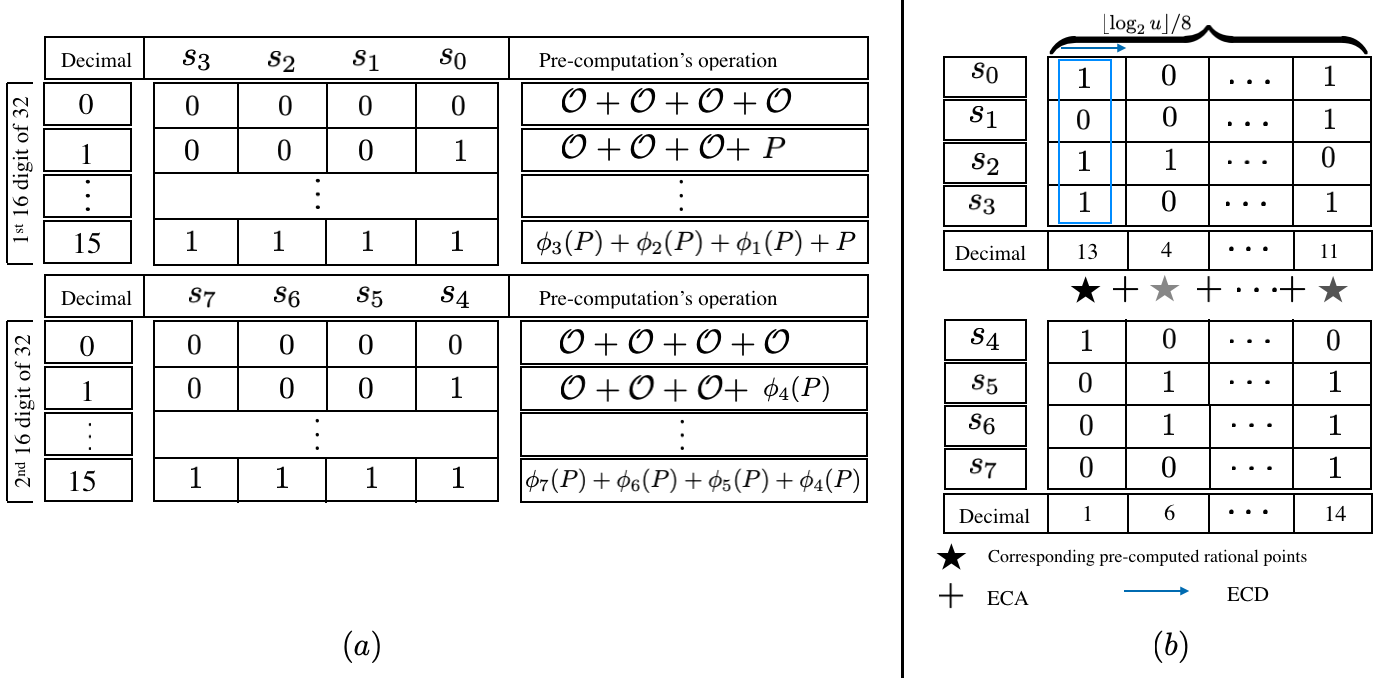
\includegraphics[width=\linewidth,height=.4\textheight, keepaspectratio]{com8split}
\caption{(a) Pre-computation of rational points for dimension 8  GLV. ~ (b) Computation of SCM for dimension 8  GLV.}
\label{precom_figure}
\end{figure*}
 Since $u = 35$-bit,  the maximum length of the scalar after the dimension 8 decomposition will be $\leq 35$-bit.
Therefore, at most 35 pre-computed points will be utilized during the  multi-scalar multiplication.
As a result, we separated the scalar into two groups as $(s_3,s_2,s_1,s_0)$ and $(s_7,s_6,s_5,s_4)$.
Then we pre-computed $2^4 + 2^4 = 32$ rational points.
\fgref{precom_figure}(a) shows the pre-computation steps.  
Among the 32 pre-computed points each of the points will be utilized at least once during multi-scalar multiplication. 
Finally, we combined the result of the two separately  obtained multi-scalar multiplication by one extra elliptic curve addition. 
%\begin{figure}[t]
%\centering
%	\includegraphics[width=\linewidth,height=.4\textheight, keepaspectratio]{com}
%%\includegraphics[scale=0.5]{com.eps}
%\caption{Computation of SCM for dimension 8  GLV.}
%\label{com_figure}
%\end{figure}
As a result we can save $2^8-32 = 224$ pre-computation. 
\fgref{precom_figure}(b) shows the computation of the loop where simultaneous multi-scalar multiplications are carried out. 

To obtain the pre-computed rational points we need to calculate $[p]Q, [p^2]Q, \cdots, [p^7]Q$ as shown in \fgref{precom_figure}(a).
Thanks to Frobenius map which can be calculated with a few multiplications in $\Fp$.
Moreover, since rational points in $\g2$ have isomorphic twisted points in $\g2'\subset E'(\FPFR)$, therefore, skew Frobenius map \cite{CANS:SNOKM08} can be applied as shown in the \secref{sec_tskew_fm}.

\subsection{Skew Frobenius Map to Compute $[p]\bar{Q'}$}
\label{sec_tskew_fm}
From the definition of $Q \in \g2$, we recall that $Q$ satisfies $[\pi_p -p]Q = \cal O$ or $\pi_p(Q) = [p]Q$, which is also applicable for $\bar{Q'}$.
Applying skew Frobenius map we can optimize $[p]\bar{Q'}$ calculation.
The detailed procedure to obtain the skew Frobenius map of $Q' = (x_{Q'}, y_{Q'}) \in \g2' \subset E'(\FPFR)$ is given bellow:
\begin{subequations}
\begin{equation}
(x_{Q'}\gamma )^p  =   (x_{Q'})^p \gamma^p. \nonumber \\
\end{equation}
After remapping 
\begin{eqnarray}
 (x_{Q'})^p \gamma^{p-1} & = &  (x_{Q'})^p (\gamma^2)^{\frac{p-1}{2}}, \nonumber
\end{eqnarray}
 \end{subequations} 
The $(\gamma^2)^{\frac{p-1}{2}} $ term can be simplified as follows:
 \begin{subequations}
 \begin{eqnarray}
 \label{gama1}
(\gamma^2)^{\frac{p-1}{2}} & = & (\beta^2)^{\frac{p-1}{4}}, \mbox{\quad since $p \equiv 5 \bmod 8$,} \nonumber \\
& = & (\alpha)^{\frac{p-1}{4} -1}\alpha, \nonumber \\
& = & (\alpha^2)^{\frac{p-5}{8}}\alpha, \nonumber \\
& = & c^{\frac{p-5}{8}}\alpha.
\end{eqnarray}
Recall that $c=2$ in \eqref{towering_1}. 
% The  $(x_{Q'})^p \in \FPFR$ can be calculated as Frobenius map in $\FPFR$  as 
% \begin{eqnarray}
% x_{Q}^p &=& (a_0+a_1\alpha+a_2\beta+a+3 \alpha\beta)^p \nonumber \\
%  & = & ( -a_1c + a_0 \alpha -a_3c \beta +a_2\alpha \beta) c^{\frac{3p-7}{8}}
% \end{eqnarray} 

Similar way the skew Frobenius map of $y_{Q'}$ is given as,
\begin{equation}\label{skewfm}
(y_{Q'}\gamma \omega )^p  =   (y_{Q'})^p \gamma^p \omega^p. \nonumber \\
\end{equation}
After remapping 
\begin{eqnarray}
 (y_{Q'})^p \gamma^{p-1} \omega^{p-1} & = &  (y_{Q'})^p (\gamma^2)^{\frac{p-1}{2}} (\omega^2)^{\frac{p-1}{2}}. \nonumber
\end{eqnarray}
 $(\gamma^2)^{\frac{p-1}{2}}$ is calculated same as \eqref{gama1}. 
 The $(\omega^2)^{\frac{p-1}{2}}$ term is calculated as follows:
\begin{eqnarray}
(\omega^2)^{\frac{p-1}{2}} & = & (\gamma^2)^{\frac{p-1}{4}},\mbox{\quad since $p \equiv 5 \bmod 8$,}\nonumber \\
& = &  \beta^{\frac{p-1}{4} -1} \beta, \nonumber \\
%& = &  ( \beta^2)^{\frac{p-5}{8}} \beta, \nonumber \\
& = &  ( \alpha)^{\frac{p-5}{8}} \beta, \nonumber \\
& = &  ( \alpha)^{\frac{p-5}{8}-1}  \alpha \beta, \nonumber \\
& = &  ( \alpha^2)^{\frac{p-13}{16}}  \alpha \beta, \nonumber \\
& = &  c^{\frac{p-13}{16}}  \alpha \beta. \nonumber
\end{eqnarray}
 \end{subequations}
 The above constant terms will be pre-calculated.
 Now the $x_{Q'})^p, (y_{Q'})^p \in \FPFR$ can be easily calculated where the coefficients will change positions and sign while multiplying with basis elements. For example  $ (x_{Q'})^p (\gamma^2)^{\frac{p-1}{2}} \in \FPFR$ can be calculated as 
%  The  $(y_{Q'})^p \in \FPFR$ can be calculated as Frobenius map in $\FPFR$ same as 
\begin{eqnarray}
 (x_{Q'})^p (\gamma^2)^{\frac{p-1}{2}} &=& (a_0+a_1\alpha+a_2\beta+a_3 \alpha\beta)^p c^{\frac{p-5}{8}}\alpha, \nonumber \\
 & = & ( -a_1c + a_0 \alpha -a_3c \beta +a_2\alpha \beta) c^{\frac{3p-7}{8}}. \nonumber
\end{eqnarray} 
Here it costs 4 multiplication in $\Fp$.
In the similar way $(y_{Q'})^p (\gamma^2)^{\frac{p-1}{2}} (\omega^2)^{\frac{p-1}{2}}$ can be calculated in costing 4 $M_p$.
Therefore, a single skew Frobenius map will cost 8 multiplications in $\Fp$.

During the pre-computation stage of GLV method we also need to compute $[p^2]Q'$, $[p^3]Q'$, $[p^4]Q'$, $[p^5]Q'$, $[p^6]Q'$, $[p^6]Q'$, and $[p^7]Q'$ skew Frobenius maps. 
The procedure is similar to computing $[p]Q'$.
Interestingly, the coefficients basis positions after the skew Frobenius map is similar for $[p]Q'$ and  $[p^5]Q'$ pair; $[p^3]Q$ and $[p^7]Q'$ pair, $[p^2]Q'$ and $[p^6]Q'$ pair.
Only the constant multiples will be different.  


%%---------------------------------Result Analysis-----------------------------
\section{Experimental Result Analysis}
To determine the advantage of the derived GLV techniques, in one hand we applied the twisted mapping to map rational point $Q \in \g2 \subset E(\F{p}{16})$ to its isomorphic point $Q' \in \g2' \subset E'(\F{p}{4})$. 
After that, we performed the scalar multiplication of $Q'$. Then the resulted points are re-mapped to $\g2$ in $\FPSN$.
On the other hand, we performed scalar multiplication using the GLV techniques derived in \secref{Proposal}.
In the experiment, 100 randomly generated scalars of size $\leq r$ (263-bit) are used to calculate SCM for all the cases.
Average value of execution time presented in the millisecond is considered for comparison.
The source of the experimental implementation can be found in Github \footnote{\footurl}.

In the experiment, KSS-16 curve over $\FPSN$ is obtained as $y^2 = x^3 + 1$ by applying the parameters  of Barbulescu et al. \cite{sylvain_new_param}  for 128-bit security level.
\tbref{environment} shows the experiment environment used for comparative evaluation. 
No optimization is done to execute the program in multithreading.
\renewcommand{\baselinestretch}{1.5}
\begin{table}[t]
\centering
\caption{Curve parameters.}
\begin{tabular}{|l|l|l|l|}
\hline
$u= 35$-bit                 & $p$      & $r$      & $t$      \\ \hline
$2^{35}-2^{32}-2^{18}+2^8+1$ & 339 -bit & 263 -bit & 270 -bit \\ \hline
\end{tabular}
\end{table}
\begin{table}[t]
	\centering
	\fontsize{8pt}{8pt}\selectfont
	\caption{Experimental Implementation Environment.}
	\label{environment}
	\resizebox{\columnwidth}{!}{
		\begin{tabular}{|l|l|l|l|l|}
			\hline
			CPU                                                                          & Memory & Compiler  & OS               & \begin{tabular}[c]{@{}l@{}}Language \&\\ Library\end{tabular} \\ \hline
			\begin{tabular}[c]{@{}l@{}}Intel(R) 2.7 GHz \\Core(TM) i5\end{tabular} & 16GB    & 4.2.1 & \begin{tabular}[c]{@{}l@{}}macOS High \\ Sierra 10.13.6\end{tabular}  &\begin{tabular}[c]{@{}l@{}}C\\GMP v 6.1.0 \cite{gmp}\end{tabular}    \\ \hline
			%	\multicolumn{6}{l}{\textsuperscript{*}\footnotesize{Only single core is used from two cores.}}\\
		\end{tabular}
	}
\end{table}
\begin{table}[t]
\centering
\caption{Maximum length of scalar $s$ after GLV decomposition in different dimensions.}
\label{s_length}
\resizebox{\columnwidth}{!}{
\begin{tabular}{|l|l|l|l|l|l|}
\hline
\multirow{2}{*}{\begin{tabular}[c]{@{}l@{}}Max bit length \\ of $s$ after GLV\end{tabular}} & \begin{tabular}[c]{@{}l@{}}Normal\\  binary\end{tabular} & 2-Split  & 2-Split JSF & 4-Split & 8-Split \\ \cline{2-6} 
                                                                                          & 263-bit                                                  & 139-bit & 139-bit    & 69-bit  & 35-bit  \\ \hline
\end{tabular}
}
\end{table}
\begin{table}[t]
	\centering
	\caption{ECD and ECA cost in $E'(\FPFR)$.}
	\label{ecaecd_fp4}
	\begin{tabular}{|l|l|}
		\hline
		ECD cost in $E'(\FPFR)$           & ECA cost in $E'(\FPFR)$  \\ \hline
		$3 M_4 + 8 A_4 + 1 I_4 + 1 M_p$ & $2 M_4 + 6 A_4 + 1 I_4$ \\ \hline
	\end{tabular}
\end{table}
\renewcommand{\baselinestretch}{1.0}
\tbref{s_length} shows the maximum bit length after applying the GLV technique on a scalar of length $263$-bit.
\tbref{ecaecd_fp4} shows the number of operation required to perform single ECA and ECD in $E'(\FPFR)$.
\tbref{tab_res_time} shows the result with respect to ECA and ECD count and time [ms].
From the results, it is clear that 4-Split is the fastest among the techniques followed by the 8-Split.
It is expected that 8-Split should be faster than the 4-Split since it's loop length is half of the 4-Split.
In other words, 8-Split requires about less than half of 4-Split's ECD during loop execution. 
However, combining two 4-Split for one 8-Split increases the number of ECA.
As a result, the total ECA count in the loop for  8-Split is almost same a 4-Split.
The significant fall back of 8-Split compared to 4-Split comes from its number of pre-computed rational points.
Moreover, the total number of pre-computation also increases the other overhead calculations such as initialization, memory allocation, padding $0$ in MSB of the decomposed scalar smaller than the max length. Which also impacts on the execution time. 
\renewcommand{\baselinestretch
}{1.4}
\begin{table}[t]
\centering
\caption{Comparative result of average execution time in [ms] for scalar multiplication.}
\label{tab_res_time}
\begin{tabular}{l|c|c|c|c|c|}
\cline{2-6}
                                    & \multicolumn{2}{l|}{Pre-computation} & \multicolumn{2}{l|}{\begin{tabular}[c]{@{}l@{}}In SCM\\ Algorithm\end{tabular}} & \multirow{2}{*}{Time {[}ms{]}} \\ \cline{1-5}
\multicolumn{1}{|l|}{Operation}     & \#ECA         & \#ECD         & \#ECA                              & \#ECD                               &                                \\ \hline
\multicolumn{1}{|l|}{Normal binary} & 0            & 0                & 120                                    & 262                         \textbf{}           & 42.81                          \\ \hline
\multicolumn{1}{|l|}{2-Split}       & 5                 	& 6                & 98                                    & 138                                     & 28.48                          \\ \hline
\multicolumn{1}{|l|}{2-Split JSF}   & 8                & 6                & 66                                    & 138                                 & 25.16                          \\ \hline
\multicolumn{1}{|l|}{4-Split}       & 24                  & 20               & 64                                     & 68                                     & 19.09                          \\ \hline
\multicolumn{1}{|l|}{8-Split}       & 52                 & 47               & 67                                     & 34                                     & 21.85                          \\ \hline
\end{tabular}
\end{table}
\renewcommand{\baselinestretch}{1.0}



\section{Conclusion}
This paper shows the detailed formula to apply the GLV decomposition together with Straus-Shamir multi-scalar multiplication technique for efficient $\g2$ scalar multiplication which is a major operation in many pairing-based protocols.
The experimental implementation confirms the correctness of the derived technique.
The comparative implementations show that dimension 4 is faster than 8 and 2. 
There is still scope to make the technique better by optimizing the pre-computation which will reduce the number of ECA and ECD.
As a future work, the authors would like to reduce the pre-computation cost by optimizing Frobenius map calculation together with the application of non-adjacent form (NAF) and evaluate the acceleration in a pairing-based protocol. 

ß


 
%\chapter{CSS 2017} 
%\title{Efficient Optimal-Ate Pairing on BLS-12 Curve Using Pseudo 8-Sparse Multiplication}

This paper shows an efficient Miller's algorithm implementation technique by applying pseudo 8-sparse multiplication over Barreto-Lynn-Scott (BLS12) curve of embedding degree 12. The recent development of exTNFS algorithm for solving discrete logarithm problem urges researchers to update parameter for pairing-based cryptography. Therefore, this papers applies the most recent parameters and also shows a comparative implementation of optimal-Ate pairing between BLS12 curve and  Kachisa-Schaefer-Scott (KSS16) curve. The result finds that pairing in BLS12 curve is faster than KSS16 although the BLS12's Miller loop parameter is twice larger than the KSS16.


\section{Introduction}
At the beginning of this century, Sakai et al. \cite{sakai2000cryptosystems} and Joux \cite{JC:Joux04} independently proposed a cryptosystem that has unlocked many novel ideas to cryptography researchers. 
Many researchers tried to find out security protocol that exploits pairings to remove the need of certification by a trusted authority. 
In this consequence, several ingenious pairing based encryption scheme such as ID-based encryption scheme by  Boneh and Franklin \cite{sakai2000cryptosystems} and group signature authentication by Nakanishi et al. \cite{AC:NakFun05} has come into the focus. 
In such outcome, Ate-based pairings such as Ate \cite{DBLP:reference/crc/2005ehcc}, Optimal-ate \cite{DBLP:journals/tit/Vercauteren10}, twisted Ate \cite{EPRINT:MKHO07} and $\chi$-Ate \cite{PAIRING:NASKM08} pairings and their applications in cryptosystems have caught much attention since they have achieved quite efficient pairing calculation.
But it has always been a challenge for researchers to make pairing calculation more efficient for being used practically as pairing calculation is regarded as quite time consuming operation. 

Generally, a pairing is a bilinear map $e$ typically defined as  $\g1 \times \g2 \to \g3$, where $\g1$ and $\g2$ are additive cyclic sub-groups of  order $r$  on a certain elliptic curve $E$ over a finite extension field $\FPK$ and $\g3$ is a multiplicative cyclic group of order $r$ over $\mF{p}{k}$.
This paper chooses an asymmetric variants of pairing named as Optimal-Ate \cite{DBLP:journals/tit/Vercauteren10} with Barreto-Lynn-Scott (BLS) \cite{SCN:BarLynSco02} pairing friendly curve of embedding degree $k=12$ named as BLS-12.

Acceleration of Optimal-Ate pairing depends not only on the optimization of Miller algorithm's loop parameter but also on efficient elliptic curve arithmetic operation and efficient final exponentiation.  
This paper has proposed a \textit{pseudo 8-sparse multiplication} to accelerate Miller's loop calculation in BLS-12 curve by utilizing the property of  rational point groups.
In addition, this papers has showed an enhancement of the elliptic curve addition and doubling calculation in Miller's algorithm by applying implicit mapping of its sextic twisted isomorphic group. 

The recent development of NFS by Kim and Barbulescu \cite{C:KimBar16} requires to update the parameter selection for all the existing pairings over the well know pairing friendly curve families such as BN \cite{SAC:BarNae05}, BLS \cite{SCN:BarLynSco02} and KSS \cite{EPRINT:KacSchSco07}.
Barbulescu and Sylvain \cite{sylvain_new_param} has proposed new parameters that for 128-bit security level and found BLS-12 is most efficient choice for Optimal-Ate pairing than well studied BN curve. Therefore the authors focuses on efficient implementation of BLS-12 curve for Optimal-Ate pairing by applying most recent parameters. 
The authors also applied final exponentiation algorithm of \cite{EPRINT:GhaFou16a} and compared the simulation result with BN with similar implementation technique.

The simulation result shows that the given \textit{pseudo 8-sparse multiplication} gives more efficient Miller's loop calculation of an Optimal Ate pairing operation along with recommended parameters than pairing calculation without sparse multiplication.

\subsection*{Related works.}
Aranha et al. \cite[Section 4]{EC:AKLGL11} and Costello et al. \cite{PKC:CosLanNae10} have  well optimized the Miller's algorithm in Jacobian coordinates by 6-sparse multiplication \footnote{\label{6sparse}{6-Sparse refers the state when in a vector (multiplier/multiplicand), among the 12 coefficients 6 of them are zero.}} for BN curve. 
Mori et al. \cite{PAIRING:MANS13} and Khandaker et al. \cite{ICISC:KONSD16} have shown  specific type of sparse multiplication for BN curve and KSS-18 curve respectively where both of the curves supports sextic twist.
It is found that pseudo 8-sparse was clearly efficient than 7-sparse and 6-sparse in Jacobian coordinates.
The authors have extended the previous works for sextic twisted BLS-12 curve.


\section{Fundamentals}
\subsection{BLS-12 curve}
Barreto, Lynn and Scott propose polynomial parameterizations by a integer variable $u$ for certain complete pairing-friendly curve families for specific embedding degrees \cite{SCN:BarLynSco02}. The target curve of this paper is such pairing-friendly curve, usually called BLS-12 of embedding degree $k-12$, defined over extension field $\FPSN$ as follows:
\begin{equation}\label{eq:KSS_16}
E/\FPTV:y^2=x^3+b, \quad \mbox{($b \in \Fp$) and  $b \neq 0$},
\end{equation}
 where $x,y \in \FPTV$. Similar to other pairing-friendly curves,  \textit{characteristic} $p$, \textit{Frobenius trace} $t$ and \textit{order} $r$ of this curve are given by the following polynomials of  integer variable $u$ also known as \textit{mother parameter}.
\begin{subequations}
\begin{eqnarray}
p(u) &= & (u-1)^2(u^4-u^2+1)/3+u,  \\\label{eq:kss_16_char}
r(u) &= & (u^4-u^2+1)\label{eq:kss_16_degree}  \\
t(u) &=& u+1, \label{eq:kss_16_trace} 
\end{eqnarray}
\end{subequations} 
where $u$ is such that $6|(p-1)$ and the $\rho$ value is $\rho = (\log_2 p/\log_2 r) \approx 1.25$. 
The total number of rational points $\#E(\Fp)$ is given by Hasse's theorem as, $\#E(\Fp) = p+1-t$. 
When the definition field is the $k$-th degree extension field $\FPK$, rational points on the curve $E$ also forms an additive Abelian group denoted as $E(\FPK)$.

\subsection{Extension Field Arithmetic and Towering}
In extension field arithmetic, higher level computations can be improved by towering. In towering, higher degree extension field is  constructed as a polynomial of lower degree extension fields.
In some previous works, such as Bailey et al. \cite{JC:BaiPaa01} explained tower of extension by using irreducible binomials. 
In what follows, Let $6|(p-1)$, where $p$ is the characteristics of BLS-12 curve and $-1$ is a quadratic and cubic non residue in $\Fp$. 
Since BLS-12 curve is defined over $\FPTV$, this paper has represented extension field  $\FPTV$ as a tower of sub-fields to improve arithmetic operations.
\begin{equation}\label{BN_towering}
\begin{cases}
\F{p}{2} = \F{p}{}[\alpha]/(\alpha^2+1),  \\ 
\F{p}{6} = \F{p}{2}[\beta]/(\beta^3-(\alpha+1)),  \\ 
\F{p}{12} = \F{p}{4}[\gamma]/(\gamma^2-\beta). \\ 
\end{cases}
\end{equation}

\subsubsection*{Extension Field Arithmetic of $\FPTV$}
Among the arithmetic operations multiplication, squaring and inversion are regarded as expensive operation than addition/subtraction. The calculation cost, based on number of prime field multiplication $M_p$ and squaring $S_p$ is given in Table \ref{tab_f12_op_count}. The algorithms for extension field operation are implemented from \cite{EPRINT:DEHR1}. The arithmetic operations in $\Fp$ are denoted as $M_p$ for a multiplication, $S_p$ for a squaring, $I_p$ for an inversion and $m$ with suffix denotes multiplication with basis element.

\begin{table*}[t]
\caption{Number of arithmetic operations in $\FPTV$ based on \eqref{BN_towering}}
\label{tab_f12_op_count}
\centering
\resizebox{\columnwidth}{!}{
\begin{tabular}{|l|l|}
\hline 
$M_{p^2} = 3M_p + 5A_p+1m_\alpha \rightarrow 3M_p $ &  $S_{p^2} = 2S_p+3A_p \rightarrow 2S_p $\\ 
$M_{p^6} = 6M_{p^2}+15A_{p^2}+2m_\beta \rightarrow 18M_p $ &  $S_{p^6} = 2M_{p^2}+3S_{p^2}+9A_{p^2}+2m_\beta \rightarrow 12S_p $\\ 
$M_{p^{12}} = 3M_{p^6}+5A_{p^6}+1m_\gamma \rightarrow 54M_p $ &  $S_{p^{12}} = 2M_{p^6}+5A_{p^6}+2m_\gamma \rightarrow 36S_p $\\ 
\hline 
\end{tabular} 
}
\end{table*}

\subsection{Optimal-Ate pairing on BLS-12 Curve}
In the context of pairing on the targeted pairing-friendly curves, two additive rational point groups $\g1, \g2$ and a multiplicative group $\g3$ of order $r$ are considered. 
$\g1$, $\g2$ and $\g3$ are defined as follows:
\begin{eqnarray}\label{eq:g1}
\g1 & = &  E(\F{p}{k}) [r] \cap \text{Ker}(\pi_p - [1]), \nonumber \\
\g2 & = &  E(\F{p}{k}) [r] \cap \text{Ker}(\pi_p - [p]), \nonumber \\
\g3 & = & \mF{p}{k}/(\mF{p}{k})^r, \nonumber \\
 e & : &\g1 \times \g2 \rightarrow \g3,
\end{eqnarray}
here $e$ denotes Optimal-Ate pairing \cite{DBLP:journals/tit/Vercauteren10}. $E(\F{p}{k})[r]$ denotes rational points of order $r$ and $[i]$ denotes $i$ times scalar multiplication for a rational point. 
$\pi_p$ denotes the Frobenius map given as $\pi_p: (x,y) \mapsto (x^p,y^p)$.

In the case of BLS-12, the above $\g1$ is just $E(\FP)$. 
In what follows, rest of this paper considers $P \in \g1 \subset E(\FP)$ and  $Q \in \g2 \subset  E(\FPTV)$ for BLS-12 curve.
Optimal-Ate pairing $e(Q,P)$ is given as follows:
\begin{equation}
	e(Q,P)=f_{u,Q}(P)^{\frac{p^{12}-1}{r}},
\end{equation}
where $f_{u,Q}(P)$ is the Miller's algorithm's result and $\lfloor \log_2 (u) \rfloor$ is the loop length. The bilinearity of Ate pairing is satisfied after calculating the final exponentiation $\frac{p^{12}-1}{r}$.


The generalized calculation procedure of Opt-Ate pairing is shown in Alg. \ref{optimal_algo}. 
In what follows, the calculation steps from 1 to 7, shown in Alg. \ref{optimal_algo}, is identified as Miller's Algorithm and step 8 is the final exponentiation. Steps 3, 5 and 7 are the line evaluation together with elliptic curve doubling (ECD) and addition (ECA) inside the Miller's loop. These line evaluation steps are the focus point of this paper for acceleration. 
The authors extended the work of \cite{PAIRING:MANS13},\cite{ICISC:KONSD16} for BLS-12 curve to calculate \textit{pseudo 8-sparse multiplication} described in Sect. 3.
The ECA and ECD are also calculated efficiently in the twisted curve. 
Step 8, FE is calculated by applying Ghammam et al.'s final exponentiation algorithm \cite{EPRINT:GhaFou16a}.

\begin{algorithm}[H]
	\caption{Optimal Ate pairing on BLS-12 curve}
	\label{optimal_algo}
	\DontPrintSemicolon

	\hspace{-3ex}
	\KwIn{$u,P\in\g1,Q'\in\g2'$}%input
\hspace{-3ex}
\KwOut{$(Q,P)$} %output
	
	\nl $f \leftarrow 1,T \leftarrow Q'$\;
	\nl \For{$i = \lfloor \log_2 (u)\rfloor $ {\bf downto} $1$} {
	\nl $f\leftarrow f^2\cdot l_{T,T}(P)$, $T\leftarrow [2]T$\;

	\nl \If{$u[i]=1$} {
	\nl $f\leftarrow f\cdot l_{T,Q'}(P)$, $T\leftarrow T+Q'$}
    \nl \If{$u[i]=-1$} {
	\nl $f\leftarrow f\cdot l_{T,-Q'}(P)$, $T\leftarrow T-Q'$}}
	\nl $f\leftarrow f^{\frac{p^{12}-1}{r}}$\;
	\nl {\bf return} $f$\;
\end{algorithm}
\vspace{-0.6em}

\subsection{Sextic Twist of BLS-12 Curve} \label{sextic_twist}
In the context of Optimal-Ate, there exists a \textit{twisted curve} with a group of rational points of order $r$, isomorphic to the group where rational point $Q \in  E(\F{p}{k}) [r] \cap \text{Ker}(\pi_p - [p])$  belongs to. This sub-field isomorphic rational point group includes a twisted isomorphic point of $Q$, typically denoted as $Q' \in E'(\FPKD)$, where $k$ is the embedding degree and $d$ is the twist degree.  

Since points on the twisted curve are defined over a smaller field than $\FPK$, therefore ECA and ECD becomes faster. 
However, when required in the Miller's algorithm's line evaluation, the points can be quickly mapped to points on $E(\FPK )$. 
Since the pairing-friendly BLS-12 \cite{SCN:BarLynSco02} curve has CM discriminant of $D = 3$ and $6|k$, therefore sextic twist is available.
Let $(\alpha+1)$ be a certain quadratic and cubic non residue in $\FPT$.  The sextic twisted curve $E_b'$ of  curve $E_b$ and their isomorphic mapping $\psi_6$ are given as follows:
\begin{eqnarray}
	E_b'&:&y^2=x^3+b(\alpha+1),\;\;\;b\in\Fp, \nonumber\\
	\psi_6&:&E_b'(\FPT)[r] \longmapsto E_b(\FPTV)[r]\cap {\rm Ker}(\pi_p-[p]),\nonumber\\
	&&(x,y)\longmapsto ((\alpha+1)^{-1}x \beta^2,(\alpha+1)^{-1}y\beta\gamma).\label{map_bn}
\end{eqnarray}
where Ker($\cdot$) denotes the kernel of the mapping and $\pi_p$ denotes Frobenius mapping  for rational point.

Table \ref{tab_Q_in12} shows a the vector representation of $Q = (x_{Q},y_Q) = (\alpha+1)^{-1}x_{Q'} \beta^2,(\alpha+1)^{-1}y_{Q'}\beta\gamma \in \FPTV$ according to the given towering in \eqref{BN_towering}. Here, $x_{Q'}$ and $y_{Q'}$ are the coordinates of rational point $Q'$ on sextic twisted curve $E'$ defined over $\FPT$. 

\renewcommand{\baselinestretch}{1.5}
\begin{table*}[t]
\caption{$\g2$ rational point  $Q = (x_Q,y_Q) \in \FPTV$  vector representation}
\label{tab_Q_in12}
\centering
\resizebox{\columnwidth}{!}{
\begin{tabular}{|*{13}{c|}}
\hline 
 & 1 & $\alpha$ & $\beta$ & $\alpha \beta$ & $\beta^2$ & $\alpha \beta^2$ & $\gamma$ & $\alpha \gamma$ & $\beta \gamma$ & $\alpha \beta \gamma$ & $ \beta^2 \gamma $ & $\alpha \beta^2 \gamma$ \\
  \hline 
$x_Q$ & 0 & 0 & 0 & 0 & $b_4$ & $b_5$ & 0 & 0 & 0 & 0 & 0 & 0 \\
 \hline 
$y_Q$ & 0 & 0 & 0 & 0 & 0 & 0 & 0 & 0 & $b_8$ & $b_{9}$ & 0 & 0 \\
\hline 
\end{tabular}
}
\end{table*}
\renewcommand{\baselinestretch}{1.0}
%-----------------------------------------------------------------------------------------------------------------------------------
\section{Proposal Overview}
%\subsection{Overview: Sparse and Pseudo-Sparse Multiplication}
Before going to the details, the overall procedure can be described as follows:
\begin{enumerate}
\item First we define the line equation for rational point $P \in E(\FP)$ and $Q', T'$ of sextic twisted curve $E'(\FPT)$.
\item Next we obtain more sparse form by multiplying $y_{P}^{-1}$ with line equations obtained at step 1.
\item To reduce the computational overhead introduced in step 2, we obtain an isomorphic map of $P \mapsto \bar{P}$ and same map for $Q \mapsto \bar{Q}$ defined over curve $\bar{E}$.
\item $\bar{Q} \in \bar{E}(\FPTV)$ is isomorphic to $E$, however it's sextic twisted $\bar{Q}$ defined over the curve $\bar{E}(\FPT)$ is not isomorphic. Therefore, we again obtain the twisted map of $\bar{Q} \in \bar{E}(\FPTV)$ to $\bar{Q'}$, defined over $\bar{E'}(\FPT)$.
\item The mapping of step 2 and 3 reduces the overhead computation and help us to achieve pseudo 8-sparse multiplication. 
\end{enumerate}

\subsection*{Obtaining line equations}
Let us consider  $T=(\gamma x_{T'},\gamma \omega y_{T'})$, $Q=(\gamma x_{Q'}, \gamma \omega y_{Q'})$  and  $P=(x_P,y_P) $, where $x_p, y_p \in \Fp$ be given in affine coordinates on the curve $E(\FPTV)$ such that $T'=(x_{T'},y_{T'})$, $Q'=(x_{Q'},y_{Q'})$ are in the twisted curve $E'$ defined over $\FPT$.
Let the elliptic curve doubling of $T+T = R(x_R, y_R)$. 
 The 7-sparse multiplication for BLS-12 can be derived as follows.
\begin{eqnarray}
 & l_{T,T}(P) = (y_p-y_{T'} (\alpha+1)^{-1}\beta\gamma)- \lambda_{T,T}(x_P-x_{T'}(\alpha+1)^{-1}\beta^2),   \quad \text{when $T = Q$,}  \nonumber\\
 &\lambda_{T,T}= \frac{ 3x_{T'}^2 \beta\gamma}{2 y_{T'} \beta^2}  = \lambda'_{T,T} \frac{\gamma}{\beta}= \lambda'_{T,T}(\alpha+1)^{-1}\beta^2\gamma
\end{eqnarray}
The line evaluation and ECD are obtained as follows:
\begin{eqnarray}
& l_{T,T}(P) = y_p+ (\lambda'_{T,T}x_{T'}- y_{T'})(\alpha+1)^{-1}\beta\gamma-\lambda'_{T,T}x_{P}(\alpha+1)^{-1}\beta^2\gamma, \nonumber \\
 & x_{2T'} = ((\lambda'_{T,T})^2  - 2x_{T'})(\alpha+1)^{-1}\beta^2 \nonumber \\
 & y_{2T'}= ((x_{T'}-x_{2T'})\lambda'_{T,T}-y_{T'})(\alpha+1)^{-1}\beta\gamma \nonumber.
\end{eqnarray}
The above calculations can be optimized as follows:
\paragraph*{Elliptic curve doubling when $T'=Q'$}
\begin{subequations}
\begin{eqnarray}
&A=\frac{1}{2y_{T'}}, B=3x_{T'}^2, C=AB, D=2x_{T'}, x_{2T'}=C^2-D,\nonumber\\
& E= Cx_{T'}-y_{T'}, y_{2T'}=E-Cx_{2T'},\nonumber\\
&l_{T',T'}(P)= y_P+(\alpha+1)^{-1}E\beta\gamma-(\alpha+1)^{-1}Cx_P\beta^2 \gamma, \label{sparse_dbl_bn_1} \\
&y_{P}^{-1}l_{T',T'}(P)= 1+(\alpha+1)^{-1}Ey_{P}^{-1}\beta\gamma-(\alpha+1)^{-1}Cx_Py_{P}^{-1}\beta^2 \gamma, \label{sparse_dbl_bn_2}
\end{eqnarray}
\end{subequations}

The elliptic curve addition phase \texorpdfstring{($T\neq Q$)}{} and line evaluation of $ l_{T,Q}(P)$ can also be optimized similar to the above procedure. Let the elliptic curve addition of $T+Q = R(x_R, y_R)$.
\begin{eqnarray}
&  l_{T,Q}(P) = (y_p-y_{T'}) (\alpha+1)^{-1}\beta\gamma- \lambda_{T,Q}(x_P-x_{T'}) (\alpha+1)^{-1}\beta^2,  \quad \text{$T \neq Q$,} \nonumber \\
&\lambda_{T,Q}= \frac{( y_{Q'}-y_{T'})(\alpha+1)^{-1}\beta\gamma}{( x_{Q'}-x_{T'})(\alpha+1)^{-1}\beta^2} = \lambda'_{T,Q} (\alpha+1)^{-1}\beta^2\gamma, \nonumber\\
& x_{R} = ((\lambda'_{T,Q})^2  \ - x_{T'} -x_{Q'})(\alpha+1)^{-1}\beta^2 \nonumber \\
 & y_{R}=(x_{T'}\lambda'_{T,Q} -x_{R'}\lambda'_{T,Q}-y_{T'})(\alpha+1)^{-1}\beta \gamma \nonumber.
\end{eqnarray}
Representing the above line equations using variables as following :
\paragraph*{Elliptic curve addition when $T' \neq Q'$ and $T'+Q'=R'(x_{R'},y_{R'})$}
\begin{subequations}
\begin{eqnarray}
&A=\frac{1}{x_{Q'}-x_{T'}}, B=y_{Q'}-y_{T'}, C=AB, D=x_{T'}+x_{Q'},\nonumber\\
 & x_{R'}=C^2-D, E= Cx_{T'}-y_{T'}, y_{R'}=E-Cx_{R'},\nonumber\\
&l_{T',Q'}(P)= y_P+(\alpha+1)^{-1}E\beta\gamma-(\alpha+1)^{-1}Cx_P\beta^2 \gamma, \label{sparse_add_bn_1} \\
&y_{P}^{-1}l_{T',Q'}(P)= 1+(\alpha+1)^{-1}Ey_{P}^{-1}\beta\gamma-(\alpha+1)^{-1}Cx_Py_{P}^{-1}\beta^2 \gamma, \label{sparse_add_bn_2}
\end{eqnarray}
\end{subequations}
 
Here all the variables $(A,B,C, D, E)$  are calculated as $\FPT$ elements.
The  position of the $y_P$, $E$ and $C$ in $\FPTV$ vector representation is defined by the basis element 1, $\beta\gamma$ and $\beta^2\gamma$ as shown in Table \ref{tab_Q_in12}. 
Therefore,  among the 12 coefficients of  $l_{T,T}(P)$ and $l_{T,Q}(P)\in \FPTV$, only 5 coefficients $y_P\in \Fp$, $Cx_Py_{P}^{-1}\in \FPT$ and $Ey_{P}^{-1}\in \FPT$ are  non-zero other 7 coefficients are zero. These zero coefficients leads to an efficient multiplication in Miller's loop usually called sparse multiplication. 

\subsection{Pseudo 8-sparse Multiplication}
The line evaluations of \eqref{sparse_add_bn_2} and \eqref{sparse_dbl_bn_2} are identical and more sparse than \eqref{sparse_add_bn_1} and \eqref{sparse_dbl_bn_1}. Such sparse form comes with a cost of computation overhead i.e., computing $y_{P}^{-1}l_{T,Q}(P)$ in the left side and $x_Py_{P}^{-1}$, $Ey_P^{-1}$ on the right. But such overhead can be minimized by the following isomorphic mapping, which also accelerates the Miller's loop iteration.
\paragraph*{Isomorphic mapping of $P \in  \g1 \mapsto \bar{P} \in \g1':$}
\begin{eqnarray}
	\bar{E}&:&y^2=x^3+b\bar{z},\nonumber\\
	&&\bar{E}(\FP)[r]\longmapsto E(\FP)[r],\nonumber\\
	&&(x,y)\longmapsto (\bar{z}^{-1}x,\bar{z}^{-3/2}y),\label{map_bn_p}
\end{eqnarray}
where $\bar{z} \in \Fp$ is a quadratic and cubic residue in $\Fp$.
The \eqref{map_bn_p} maps rational point $P$ to $\bar{P}(x_{\bar{P}},y_{\bar{P}})$ such that $(x_{\bar{P}},y_{\bar{P}}^{-1})=1$.
The twist parameter $\bar{z}$ is obtained as:
\begin{equation}\label{z_bn}
\bar{z}=(x_Py_P^{-1})^6
\end{equation}
From the \eqref{z_bn} $\bar{P}$ and $\bar{Q'}$ is given as
\begin{subequations}
\begin{eqnarray}
\bar{P}(x_{\bar{P}}, y_{\bar{P}})&=& (x_P z^{-1},y_P z^{-3/2}) =(x_P^3y_P^{-2},x_P^3y_P^{-2}) \label{P_hat} \\ 
\bar{Q'}(x_{\bar{Q'}}, y_{\bar{Q'}})&=&(x_P^2y_P^{-2}x_{Q'},x_P^3y_P^{-3}y_{Q'}) \label{Q_hat}
\end{eqnarray}
\end{subequations}
 Using \eqref{P_hat} and \eqref{Q_hat} the line evaluation of \eqref{sparse_dbl_bn_2} becomes 
 \begin{subequations}
\begin{eqnarray}
y_{\bar{P}}^{-1}l_{\bar{T'},\bar{T'}}(\bar{P})&=& 1+(\alpha+1)^{-1}Ey_{\bar{P}}^{-1}\beta\gamma-(\alpha+1)^{-1}Cx_{\bar{P}}y_{\bar{P}}^{-1}\beta^2 \gamma, \nonumber \\
\bar{l}_{\bar{T'},\bar{T'}}(\bar{P})&=& 1+(\alpha+1)^{-1}E(x_{P}^{-3} y_{P}^{2})\beta\gamma-(\alpha+1)^{-1}C\beta^2 \gamma. 
\label{psparse_dbl_bn_2} 
\end{eqnarray}
\end{subequations}
The \eqref{sparse_add_bn_2} becomes similar to \eqref{psparse_dbl_bn_2}.
However, the to get the above form we need the following pre-computations once in every Miller's Algorithm execution.
\begin{itemize}
\item Computing $\bar{P}$ and $\bar{Q'}$,
\item $(x_{P}^{-3} y_{P}^{2})$
\end{itemize}
The $(\alpha+1)^{-1}$ can precomputed once since it is just inversion of the basis element.
The above terms can be computed from $x_{P}^{-1}$ and $y_P^{-1}$ by utilizing Montgomery trick \cite{mont_trick}, as shown in \textbf{Alg.} \ref{pre_calc_Algo}. 
The pre-computation requires 21 multiplication, 1 squaring and 1 inversion in $\Fp$ and 2 multiplication, 3 squaring  in $\FPFR$.

\begin{algorithm}[H]
	\caption{Pre-calculation and mapping $P \mapsto\bar{P}$ and $Q'\mapsto \bar{Q'}$}
	\label{pre_calc_Algo}
	\DontPrintSemicolon
	\hspace{-3ex}
	\KwIn{$P=(x_P,y_P) \in\g1,Q'=(x_{Q'},y_{Q'})\in\g2'$}%input
\hspace{-3ex}
\KwOut{$\bar{Q'},\bar{P},y_{P}^{-1}$} %output
	
	\nl $A \leftarrow (x_Py_P^{-1})$\;
    \nl $B \leftarrow Ax_P^{2}$\;
    \nl $C \leftarrow Ay_P$\;
    \nl $D \leftarrow Dx_{Q'}$\;
    \nl $x_{\bar{Q'}} \leftarrow Dx_{Q'}$\;
    \nl $y_{\bar{Q'}} \leftarrow BDy_{Q'}$\;
    \nl $x_{\bar{P}}, y_{\bar{P}} \leftarrow Dx_P$\;
    \nl $y_P^{-1} \leftarrow C^3y_{P}^2$\;
	\nl {\bf return} $\bar{Q'}=(x_{\bar{Q'}},y_{\bar{Q'}}),\bar{P} = (x_{\bar{P}}, y_{\bar{P}}), y_{P}^{-1}$\;
\end{algorithm}
\vspace{-0.6em}


Finally, pseudo 8-sparse multiplication for  BLS-12 is given in 
\begin{algorithm}[htbp]
	\caption{Pseudo 8-sparse multiplication for BLS-12 curves}
	\label{sparse_mul}
	\DontPrintSemicolon

	\hspace{-3ex}
	\KwIn{$a,b\in \Fpxii$\\
	$a=(a_0+a_1\beta+a_2\beta^2)+(a_3+a_4\beta+a_5\beta^2)\gamma$, $b=1+b_4\beta\gamma+b_5\beta^2\gamma$\\
	{\bf where} $a_i,b_j, c_i\in \Fpii(i=0,\cdot\cdot\cdot,5,j=4,5)$}%input
	\hspace{-3ex}
	\KwOut{$c=ab=(c_0+c_1\beta+c_2\beta^2)+(c_3+c_4\beta+c_5\beta^2)\gamma\in \Fpxii$} %output
	%
	\nl $c_4\leftarrow a_0\times b_4$, $t_1\leftarrow a_1\times b_5$, $t_2\leftarrow a_0+a_1$, $S_0\leftarrow b_4+b_5$\;
	\nl $c_5\leftarrow t_2\times S_0-(c_4+t_1)$, $t_2\leftarrow a_2 \times b_5$, $t_2 \leftarrow t_2 \times (\alpha+1)$\;
	\nl $c_4\leftarrow c_4+t_2$, $t_0 \leftarrow a_2 \times b_4$, $t_0 \leftarrow t_0+t_1$\;
	\nl $c_3 \leftarrow t_0 \times (\alpha+1)$, $t_0\leftarrow a_3 \times b_4$, $t_1\leftarrow a_4\times b_5$, $t_2\leftarrow a_3+a_4$\;
	\nl $t_2 \leftarrow t_2 \times S_0-(t_0+t_1)$\;
	\nl $c_0 \leftarrow t_2 \times (\alpha+1)$, $t_2 \leftarrow a_5 \times b_4$, $t_2 \leftarrow t_1+t_2$\;
	\nl $c_1 \leftarrow t_2 \times (\alpha+1)$, $t_1 \leftarrow a_5 \times b_5$, $t_1 \leftarrow t_1 \times (\alpha+1)$\;
	\nl $c_2 \leftarrow t_0+t_1$\;
	\nl $c\leftarrow c+a$\;
	\nl return $c=(c_0+c_1\beta+c_2\beta^2)+(c_3+c_4\beta+c_5\beta^2)\gamma$
\end{algorithm}

\vspace{-0.6em}

\subsection{Final Exponentiation}
%\subsubsection*{Final exponentiation of KSS-16 curve}
Scott et al. \cite{PAIRING:SBCDK09a} shows efficient final exponentiation $f^{p^k-1/r}$ by decomposing it using cyclotomic polynomial $\Phi_{k}$ as 
\begin{equation}\label{scott_dec}
(p^k-1)/r = (p^{k/2}-1) \cdot(p^{k/2}+1)/\Phi_{k}(p)\cdot \Phi_{k}(p)/r
\end{equation}
Here, the 1st 2 terms of the right part is denoted as easy part, since it can be easily calculated by Frobenius mapping and 1 inversion in affine coordinates. 
The last term is called hard part which mostly effects the computation performance.
According to \eqref{scott_dec}, the exponent decomposition of the BLS-12 curve is shown in \eqref{bls_final}.
\begin{equation}\label{bls_final}
(p^{12}-1)/r = (p^{6}-1) \cdot(p^{2}+1)\cdot (p^4-p^2+1)/r
\end{equation}
To efficiently carry out FE for the target curves we applied $p$-adic representation as shown in \cite{EPRINT:GhaFou16a}.
For scalar multiplication by prime $p$, i.e., $p[Q]$ or $[p^2]Q$, skew Frobenius map technique by Sakemi et al. \cite{CANS:SNOKM08} has been adapted.

\section{Experimental result evaluation}
This gives details of the experimental implementation.
Table \ref{exp_tab} shows implementation environment.  
\renewcommand{\baselinestretch}{1.5}
\begin{table}[htb]
\centering
\caption{Computational Environment}
\label{exp_tab}
\resizebox{\columnwidth}{!}{
\begin{tabular}{|l|c|l|l|c|l|}
\hline
CPU{\textsuperscript{*}}                                                                               & Memory & Compiler  & OS               & Language & Library     \\ \hline
\begin{tabular}[c]{@{}l@{}}Intel(R) Core(TM)\\ i5-6500 CPU @ 3.20GHz\end{tabular} & 4GB    & GCC 5.4.0 & Ubuntu 16.04 LTS & C        & GMP v 6.1.0 \cite{gmp} \\ \hline
\multicolumn{6}{l}{\textsuperscript{*}\footnotesize{Only single core is used from two cores.}}\\
\end{tabular}
}
\end{table}
\renewcommand{\baselinestretch}{1.0}
Parameters chosen from \cite{sylvain_new_param} is shown in Table \ref{parameters}.
\renewcommand{\baselinestretch}{1.5}
\begin{table}[htb]
\caption{Selected parameters for 128-bit security level \cite{sylvain_new_param}}
\label{parameters}
\begin{center}		 
\resizebox{\columnwidth}{!}{
\begin{tabular}{|l|l|c|c|c|c|c|}
\hline
Curve & ~~~~~~~~~~~~~$u$& HW(u) & $\lfloor\log_2 u \rfloor$ & $\lfloor\log_2 p(u) \rfloor$ & $\lfloor\log_2 r(u) \rfloor$& $\lfloor\log_2 p^k \rfloor$ \\ \hline
BN & $u=2^{114}+2^{101}-2^{14}-1$ & $4$& $115$ & $462$ & $462$& $5535$\\ \hline
BLS-12 & $u=-2^{77}+2^{50}+2^{33}$ & $3$& $77$ & $461$ & $308$& $5532$\\ \hline
\end{tabular}
}
\end{center}
\end{table}
\renewcommand{\baselinestretch}{1.0}
Table \ref{result_table} shows execution time in millisecond for a single Opt-Ate pairing. Results here are the average of 10 pairing.
\renewcommand{\baselinestretch}{1.5}
\begin{table}[htb]
\centering
\caption{Comparative results of Miller's Algorithm and Final Exp. in [ms]}
\label{result_table}
%\resizebox{\columnwidth}{!}{
\begin{tabular}{l|l|l|l|}
\cline{2-4}
                             & \multicolumn{3}{c|}{Pairing}      \\ \cline{2-4} 
                             & Miller Algo. & Final Exp. & Total time [ms] \\ \hline
\multicolumn{1}{|l|}{BN}     & 7.53         & 20.63      &    \textbf{28.16}   \\ \hline
\multicolumn{1}{|l|}{BLS-12} & 9.93        & 37.05      &     46.98  \\ \hline
\end{tabular}
%}
\end{table}
\renewcommand{\baselinestretch}{1.0}
Table \ref{operation_count} shows complexity of Miller's algorithm and final exponentiation. 
From the results we find that Miller's algorithm took least time for BN curve and Most for BLS-12. 
However, the time differences for the Miller's algo. among the curves are not significant as final exponentiation. The major difference is made by the calculation of hard part of the final exp. 
\renewcommand{\baselinestretch}{1.5}
\begin{table}[htb]
\centering
\caption{Operation count in $\Fp$ for 1 single pairing operation}
\label{operation_count}
\begin{tabular}{cl|l|l|l|l|l|}
\cline{3-7}
                                              &                & Multiplication & Squaring     & \begin{tabular}[c]{@{}l@{}}Addition/\\ Subtraction\end{tabular} & \begin{tabular}[c]{@{}l@{}}Basis\\ multiplication\end{tabular} & Inversion    \\ \hline
\multicolumn{1}{|c|}{\multirow{3}{*}{BN}}     & Miller's Algo. & 10957          & 157          & 35424                                                           & 3132                                                           & 125          \\ \cline{2-7} 
\multicolumn{1}{|c|}{}                        & Final exp.     & 29445          & 25           & 126308                                                          & 9808                                                           & 1            \\ \cline{2-7} 
\multicolumn{1}{|c|}{}                        & Total          & 40402          & 182          & 161732                                                          & 12940                                                          & \textbf{126} \\ \hline
\multicolumn{1}{|c|}{\multirow{3}{*}{BLS-12}} & Miller's Algo. & 7178           & 183          & 23768                                                           & 857                                                            & 81           \\ \cline{2-7} 
\multicolumn{1}{|c|}{}                        & Final exp.     & 25708          & 2            & 111157                                                          & 3832                                                           & 1            \\ \cline{2-7} 
\multicolumn{1}{|c|}{}                        & Total          & 32886          & 185          & 134925                                                          & 4689                                                           & 82           \\ \hline
\end{tabular}
\end{table}
\renewcommand{\baselinestretch}{1.0}


 //CHECK table

%%%\part{Works}
%\chapter{ICCE-TW 2016} 
%\chapter{ICCE-TW 2016} 

In elliptic curve cryptography (ECC), a scalar multiplication for rational point is the most time consuming operation. This paper proposes an efficient calculation for a scalar multiplication by applying Frobenious Mapping. Particularly, this paper deals with  Barreto-Naehrig curve defined over extension field $\F{q}{2}$, where $q=p^6$ and $p$ is a large prime.

%Scalar multiplication of rational points on elliptic curve (EC) is the most time costly operation carried out in elliptic curve cryptography (ECC). In this paper an efficient way to calculate the scalar multiplication is proposed by applying Frobenious Mapping (FM) on the rational points on Barreto - Naehrig (BN) curve. This paper considers the BN curve to be defined over extension field $\F{q}{2}$ for a very large value of $p$.

\section{Introduction}
%Since the inception of elliptic curve cryptography (ECC) it has gained wide acceptance mostly due to its smaller key size and greater security. 
%The equation of elliptic curve is defined as
% \begin{equation}\label{eq:eccdef}
%E:y^2 = x^3 + ax + b,
% \end{equation}
% where $4a^3 + 27b^2 \neq 0$. 
In cryptography research, elliptic curve cryptography (ECC) has gained a wide acceptance due to its smaller key size and greater security. 
In ECC, scalar multiplication (SM) is carried out at the encryption and decryption phases. SM is the major operation in ECC. Let us denote a scalar and rational point by  $s$ and $P$, respectively. Then, the SM is denoted by $[s]P$. In real cases $s$ is significantly large number less than the order of rational point group. Since SM needs a complicated calculation over the definition field such as prime field, an efficient algorithm for SM is needed. Recently, ECC defined over extension field $\F{q}{2}$ with a large prime number $p$ such as more than $2000$ bits is used in some ECC based protocols. On the other hand, pairing based cryptography realizes some innovative application protocol. Pairing based cryptography requires pairing friendly curve which is difficult to generate. Barreto-Naehrig (BN) \cite{BN} curve is one of the well known pairing friendly curve\cite{BN_def} whose parameters are able to be systematically given. BN curve is mostly used due to its efficiency to realize pairing based cryptography. Thus, this paper proposes an efficient approach for calculating SM on BN curve particularly defined over extension field $\F{q}{2}$, where $q=p^6$ and $p$ is a prime number by using Frobenious Mapping (FM) for the rational points.
 
\section{Preliminaries}
This section briefly discusses the fundamental arithmetic operations required for elliptic curve cryptography defined over prime field $\Fp$ and its extension field $\F{q}{2}$. In addition, this paper focuses on BN curve defined over $\F{q}{2}$, $q=p^6$.

\subsection{BN curve over prime field $\Fp$}
BN curve is a non\- super-singular (\textit{ordinary}) pairing friendly 
elliptic curve of embedding degree 12\cite{BN_def}. The equation of BN curve defined over $\Fp$ is given by 
\begin{equation}\label{eq:(BN_curve)}
E:y^2=x^3+b, \quad \mbox{($b \in \Fp$)}.
\end{equation}
where $b \neq 0$. Its characteristic $p$, Frobenius trace $t$ and order $r$ are given by using an integer variable $\chi$ as follows:
\begin{eqnarray}
p(\chi) & = & 36\chi^4-36\chi^3+24\chi^2-6\chi+1, \\
r(\chi) & = & 36\chi^4-36\chi^3+18\chi^2-6\chi+1,\label{eq:bn_degree}  \\
t(\chi) & = & 6\chi^2+1.\label{eq:bn_trace} 
\end{eqnarray} 
From \eqref{eq:bn_degree} and \eqref{eq:bn_trace} we find that the bit size of $r$ is two times larger than $t$. Thus, these parameters generally satisfy $t \ll p \approx r$ and the following relation.
\begin{equation}\label{eq:rpt_relation}
r = p+1-t.
\end{equation}

\subsubsection{Point addition}Let $E(\f{p})$ be the set of all rational points on the curve defined over $\f{p}$ and it includes the point at infinity denoted by $\mathcal{O}$.
Let us consider two rational points $P = (x_P, y_P)$, $Q = (x_Q, y_Q)$, and their addition $R = P + Q$, where $\textit{R} = (x_R, y_R)$ and $P, Q, R\in E(\Fp)$. Then, the $x$ and $y$ coordinates of $R$ is calculated as follows.
\begin{subequations}
\begin{equation}\label{eq:point_solpe}
\lambda = 
\begin{cases}
 \frac{y_Q-y_P}{x_Q-x_P} \quad \mbox{($P \neq Q$ and $x_Q \neq x_P$)},\\
  \frac{3x_P^2}{2y_P} \quad  \mbox{($P = Q$ and $y_P\neq 0$)} ,\\
  \phi \quad \mbox{otherwise.}
\end{cases}
\end{equation}

\begin{eqnarray}\label{eq:point_add}
(x_R ,y_R) & = & ((\lambda^2-x_P-x_Q ),\nonumber \\ 
&  &     (x_P-x_R)\lambda-y_P), \mbox{ if $\lambda \neq 0$}.  \\	
(x_R ,y_R) & = & \cal O \quad \mbox{if $\lambda = 0$}.
\end{eqnarray}
\end{subequations}
$\lambda$ is the tangent at the point on EC and $\cal O$ it the additive unity in $E(\f{p})$. When $P=-Q$ then $P+Q=\cal O$ is called elliptic curve addition (ECA). If $P=Q$ then $P+Q=2R$, which is known as elliptic curve doubling (ECD). 


\subsection{Elliptic curve over extension field $\F{q}{2}$}
At first, let us consider arithmetic operations in $\F{q}{2}$, which is the degree $2$ extension field over $\Fq$. In other words extension field $\F{q}{2}$ is the two dimensional vector space over $\Fq$. Let $\left\lbrace v_0, v_1 \right\rbrace $ be a basis of $\F{q}{2}$, an arbitrary element $\textbf{x} \in \F{q}{2}$ is represented as
\begin{equation}\label{eq:vector_withbasis}
\textbf{x} = x_0v_0 +x_1v_1, \ \mbox{ where $x_i \in \Fq$}.
\end{equation} 
When we implicitly know the basis vectors $v_0$ and $v_1$, \eqref{eq:vector_withbasis} is simply expressed as

\begin{equation}\label{eq:vector_reprentation}
\textbf{x} = (x_0,x_1).
\end{equation}

\subsubsection{Addition and subtraction in $\F{q}{2}$}
For vectors, addition, subtraction, and multiplication by a scalar in $\f{q}$ are carried out by coefficient wise operations over $\f{q}$. Let us consider two vectors $\textbf{x}=(x_0,x_1)$ and $\textbf{y}=(y_0,y_1)$. Then,
\begin{eqnarray}
\textbf{x} \pm \textbf{y} & = &  (x_0 \pm y_0, x_1 \pm y_1), \\
k\textbf{x} & = &  (kx_0,  kx_1),  \mbox{ $k \in \Fq$}.
\end{eqnarray}
 
\subsubsection{Vector multiplication in $\F{q}{2}$}
For a vector multiplication, we simply consider a polynomial basis representation. Let  $f(x)$ be an irreducible polynomial of degree 2 over $\Fq$. Particularly, an irreducible binomial is efficient for calculations. In order to obtain an irreducible binomial, Legendre Symbol $\Leg{c}{q}$ is useful. Consider a non-zero element $c \in \Fq$. If $c$ does not have square roots, $f(x) =x^2 - c$ becomes an irreducible binomial over $\Fq$. In order to judge it, Legendre symbol is generally applied. Then, let its zero be $\omega$, $\omega \in \F{q}{2}$, the set $\left\lbrace 1,\omega \right\rbrace $ forms a polynomial basis in $\F{q}{2}$. Using this polynomial basis, the multiplication of two arbitrary vectors is performed as follows:
\begin{eqnarray}
\textbf{xy} & = & (x_0+x_1\omega)(y_0+y_1\omega)\nonumber\\
& = & x_0 y_0 + (x_0 y_1+x_1 y_0)\omega +x_1y_1\omega^2 \nonumber \\ 
& = &(x_0 y_0 + c x_1 y_1)+ (x_0 y_1+x_1 y_0)\omega.
\end{eqnarray}
In this calculation, we have substituted $\omega^2 - c = 0$, since $\omega$ is a zero of the irreducible binomial $f(x)=x^2-c$.

\subsubsection{Vector inversion in $\F{q}{2}$}
For calculating the multiplicative inverse vector of a non-zero vector $\textbf{x}\in \F{q}{2}$, first we calculate the conjugate of $\textbf{x}$ that is given by  Frobenius mapping (FM)
$\pi_q(\textbf{x}) = \textbf{x}^q$. In detail, $\pi_q(\textbf{x})=\textbf{x}^q$ is the conjugate of $\textbf{x}$ to each other. Then the inverse $\textbf{x}^{-1}$ of \textbf{x} is calculated as follows.
\begin{equation}
\textbf{x}^{-1} = n(\textbf{x})^{-1}(\textbf{x}^q), \label{InvCal}
\end{equation}
where  $\textbf{x}$, $\textbf{x}^q$ are the conjugates and $n(\textbf{x}) \in \mFq$ is their
product. FM of $\textbf{x}$, $\pi_q(\textbf{x}) =  (x_0+x_1\omega)^q$ can be easily calculated using an irreducible binomial as follows:
\begin{eqnarray}\label{eq:FM}
(x_0+x_1\omega)^q & = & \sum_{i=0}^{q} {q\choose i} x_0^{(q-i)}(x_1\omega)^i \nonumber\\
%& = & x_0^p + (x_1\omega)^p \nonumber\\
& = & x_0 + x_1\omega^q  \nonumber \\
%\end{eqnarray}
%We can easily calculate $\omega^p$ as follows:
%\begin{eqnarray}\label{eq:omega}
%\omega^p & = & \omega^{p-1} \omega\nonumber\\
& = & x_0+x_1(\omega^2)^{\frac{q-1}{2}}\omega \nonumber \\ 
& = & x_0+x_1(c)^{\frac{q-1}{2}}\omega \nonumber \\
& = & x_0-x_1\omega,
\end{eqnarray}
where we substituted the modular relation $\omega^q = - \omega $. In other words, the conjugate of $\textbf{x}$ is given as $x_0 - x_1\omega$. Therefore, the calculation procedure for $n(\textbf{x}) = \textbf{x}\pi_q(\textbf{x})$ is as follows:
\begin{eqnarray}\label{eq:Inversion}
n(\textbf{x}) & = & (x_0+x_1\omega)(x_0 -x_1\omega)\nonumber\\
& = & x_0^2 - x_1^2\omega^2 \nonumber \\ 
& = & x_0^2 - cx_1^2.
\end{eqnarray}
Since $n(\textbf{x})$ is given without $\omega$, it is found that $n(\textbf{x})$ is a scalar. Finally, the inversion \eqref{InvCal} is efficiently calculated.


\section{Efficient scalar multiplication}
In the context of pairing-based cryptography especially on BN curve, three groups $\g1, \g2$, and $\mathbb{G}_T$ are considered. Among them, $\g1, \g2$ are rational point groups and $\mathbb{G}_T$ is the multiplicative group in the extension field. They have the same order $r$. Let us consider a rational point $Q\in \g2 \subset E(\F{q}{2})$ as $Q(\textbf{x},\textbf{y}) =(x_0+x_1\omega, y_0+y_1\omega)$. In the case of BN curve, it is known that $Q$ satisfies the following relations:
\begin{eqnarray}\label{eq:Q_rel1}
\big[p+1-t\big]Q & = & \cal O \nonumber \\
\big[t-1\big]Q  & = & \big[p\big]Q.
\end{eqnarray}
\begin{eqnarray}\label{eq:Q_rel2}
[\pi_p -p]Q & = &\cal O \nonumber \\
\pi_p(Q) & = & [p]Q.
\end{eqnarray}
Thus, these relations can accelerate a scalar multiplication in $\g2$. From \eqref{eq:Q_rel2} $\pi_p(Q)= [p]Q$. Substituting $[p]Q$ in \eqref{eq:Q_rel1} we find $[t-1]Q = \pi_p(Q)$. 
%The FM of $Q$, $\pi(Q)$ can be easily computed according to \eqref{eq:FM} as 
%\begin{equation}
%\pi(Q)= (x_0 -x_1\omega, y_0-y_1\omega). 
%\end{equation}
Next, let us consider SM $[s]Q$, where $0 \leq s \leq r$. From \eqref{eq:bn_degree} we know $r$ is the order of BN curve  where $[r]Q=\cal O$. Here, the bit size of $s$ is nearly equal to $r$. As previously said, in BN curve $r$ is two times larger than the bit size of $t$. It means that $s$ is two times larger than the bit size of $t-1$. Therefore, let us consider $[t-1]$-adic representation of $s$ as $s = s_0+s_1(t-1)$, where $s$ will be separated into two coefficients $s_0$ and $s_1$ whose size will be nearly equal to or less than the size of $[t-1]$. Then SM  $[s]Q$ is calculated as follows:
\begin{eqnarray}\label{eq:scalar_mul_Q}
[s]Q & =  & [s_0]Q+[s_1(t-1)]Q \nonumber \\
& =  & [s_0]Q+s_1\pi_p(Q).
\end{eqnarray}
Then, applying a multi-scalar multiplication technique, the above calculation will be efficiently carried out.

\section{Conclusion and future work}
%\lipsum[6]
In this paper, we have introduced an acceleration of scalar multiplication on Barreto-Naehrig (BN) curve defined over 2 degree extension field $\F{q}{2}$, $q=p^6$. We have showed that $[t-1]$-adic representation of large scalar number along with Frobenius mapping (FM) on rational points accelerates SM operation significantly, where $t$ is the Frobenius trace of BN curve. As a future work, we would like to evaluate its computational time with a large prime characteristic as a practical situation.


\begin{thebibliography}{1}

\bibitem{BN}
Paulo S. L. M. Barreto and M. Naehrig, ``Pairing-friendly elliptic curves of prime order," Selected Areas in Cryptography, 12th International Workshop, SAC 2005, Kingston, ON, Canada, August 11-12, 2005, Revised Selected Papers, pages 319-331, 2005. Springer LNCS 3897 (2006).
\bibitem{BN_def}
D. Freeman, M. Scott, and E. Teske, ``A taxonomy of pairing-friendly elliptic curves," Cryptography ePrint Archive, Report 2006/372 (2006), http://eprint.iacr.org/2006/372
\bibitem{chibasedBN}
Y. Nogami, M. Akane, Y. Sakemi, H. Katou, and Y. Morikawa, ``Integer Variable chi-Based Ate Pairing," Pairing- Based Cryptography - Pairing 2008, Second International Conference, Egham, UK, September 1-3, 2008. Proceedings, pages 178-191, 2008. Springer LNCS 5209 (2008).


\end{thebibliography}


 % NO NEED
%\chapter{ITC CSCC 2017} 
%% \documentclass[10pt,compsoc,conference, letterpaper]{IEEEtran}
% %\documentclass[10pt,compsoc]{IEEEtran}
% %\usepackage[letterpaper, total={7in, 1in}]{geometry}
% \usepackage{geometry}
% \geometry{
%  letterpaper,
%  top=2.2truecm,
% left=2truecm,
% bottom=2.6truecm,
% right = 2truecm,
% }

% \usepackage{cite}
% %\usepackage{filecontents,lipsum}
% \usepackage{nogamacro}
% %\setcounter{page}{1}
% \usepackage{amsfonts}
% \usepackage{amsmath}
% \usepackage{amssymb}
% % *** MATH PACKAGES ***
% \usepackage{amsmath}
% % *** SPECIALIZED LIST PACKAGES ***
% \usepackage{algorithmic}
% % *** ALIGNMENT PACKAGES ***
% \usepackage{array}
% \usepackage{mdwmath}
% \usepackage{mdwtab}
% \usepackage{eqparbox}
% \usepackage[makeroom]{cancel}
% \usepackage{url}
% % *** SUBFIGURE PACKAGES ***
% %\usepackage[tight,footnotesize]{subfigure}
% \usepackage{caption}
% \usepackage[font=md, labelfont=bf]{caption}
% % correct bad hyphenation here
% \hyphenation{op-tical net-works semi-conduc-tor}


% %%%%%%%%%%%%%%%%%%%%%%%%%%%%%%%%%%%%%%%%%%%%%%%%%%%%%%%%
% \newcommand{\keyword}[1]{\par\addvspace\baselineskip
% \noindent\textbf{Keywords:}\enspace\ignorespaces #1}

% \newcommand{\FP}{\mathbb{F}_p}
% \newcommand{\EFQ}{E(\mathbb{F}_q)}
% \newcommand{\EFP}{E(\mathbb{F}_p)}
% \newcommand{\SEFQ}{\#E(\mathbb{F}_q)}
% \newcommand{\SEFP}{\#E(\mathbb{F}_p)}
% \newcommand{\FPK}{\mathbb{F}_{p^k}}
% \newcommand{\FPKD}{\mathbb{F}_{p^{k/d}}}
% \newcommand{\FPTH}{\mathbb{F}_{p^3}}
% \newcommand{\FPTHTW}{\mathbb{F}_{(p^3)^2}}
% \newcommand{\FPTHTWTH}{\mathbb{F}_{((p^3)^2)^3}}
% \newcommand{\FPSX}{\mathbb{F}_{p^6}}
% \newcommand{\FPTV}{\mathbb{F}_{p^{12}}}
% \newcommand{\FPEN}{\mathbb{F}_{p^{18}}}
% \newcommand{\GT}{\mathbb{G}_T}

% \newcommand{\FPT}{\mathbb{F}_{p^2}}
% \newcommand{\FPTT}{\mathbb{F}_{(p^2)^2}}
% \newcommand{\FPTTT}{\mathbb{F}_{((p^2)^2)^2}}
% \newcommand{\FPTTTT}{\mathbb{F}_{(((p^2)^2)^2)^2}}
% \newcommand{\FPFR}{\mathbb{F}_{p^4}}
% \newcommand{\FPET}{\mathbb{F}_{p^{8}}}
% \newcommand{\FPSN}{\mathbb{F}_{p^{16}}}
%%%%%%%%%%%%%%%%%%%%%%%%%%%%%%%%%%%%%%%%%%%%%%%%%%%%%%%%

%\newgeometry{top=1.0cm,bottom=1.0cm}
%\newgeometry{left=2.0cm,right=2.00cm}
\title{Frobenius Map and Skew Frobenius Map for Ate-based Pairing over KSS Curve of Embedding Degree 16}

In pairing-based cryptography, scalar multiplication is often regarded as one of the major bottlenecks for faster pairing calculations. Frobenius map and skew Frobenius map over the twisted curve, are common techniques to speed up scalar multiplication in a pairing calculation. This paper explicitly shows the detailed procedure to calculate the Frobenius map and skew Frobenius map and their computational complexity in the context of Ate-based pairing over Kachisa-Schaefer-Scott (KSS) curve of embedding degree 16.


\section{Introduction}
Pairing-based cryptography is regarded as the basis of next generation security protocols. From the very beginning, it attracts many researchers which offered us many innovative security protocols till this date. 
But still there exist several major challenges such as efficiently carry out Miller's algorithm, final exponentiation, efficient scalar multiplication and so on, to practically use pairing in cryptography. Among several optimization techniques,  the Frobenius mapping is well-known for efficient scalar multiplication. Sakemi et al. \cite{sakemi_skew} have shown a technique named as skew Frobenius map in a twisted curve for efficiently calculating scalar multiplication.

The main focus of this paper is to explicitly show the implementation procedure of  Frobenius map and skew Frobenius map for KSS curve of embedding degree 16 (KSS16) in the context of optimal Ate pairing. This paper also gives some comparative study between this two procedures. Recently Ghammam et al. \cite{kss_lub} have proposed that KSS16 curve is a strong candidate to implement pairing-based cryptography at 192-bit security level. Therefore the authors selected KSS16 curve to obtain the skew Frobenius map over the quartic twisted curve. Moreover, to our knowledge, till this date, no work has been proposed for efficiently calculating scalar multiplication over KSS16 curve using skew Frobenius map. This paper will give a clear outline to utilize skew Frobenius map for efficient scalar multiplication.

\section{Preliminaries}
Fundamentals of KSS curve and  optimal Ate pairing are briefly given in this section.
\subsection{Kachisa-Schaefer-Scott (KSS) curve \cite{kss}}
 In  \cite{kss}, Kachisa, Schaefer, and Scott proposed a family of non super-singular Brezing-Weng pairing friendly elliptic curves using the elements in the cyclotomic field.  In what follows, this papers considers \textit{KSS16} curve of embedding degree $k =16$, defined over $\FPSN$ as follows:
\begin{equation}\label{eq:KSS_16}
E/\FPSN:Y^2=X^3+aX, \quad \mbox{($a \neq 0 \in \Fp$) },
\end{equation}
 where $X,Y \in \FPSN$. Its characteristic $p$, Frobenius trace $t$ and order $r$ are given by the integer variable $u$ as follows:
\begin{subequations}
\begin{eqnarray}
p(u) &= & (u^{10} +2u^9 +5u^8 +48u^6 +152u^5 +240 \nonumber \\
&&u^4+625u^2 +2398u+3125)/980,  \\\label{eq:kss_16_char}
r(u) &= & u^8 +48u^4 +625,\label{eq:kss_16_degree}  \\
t(u) &=& (2u^5 +41u+35)/35, \label{eq:kss_16_trace} 
\end{eqnarray}
\end{subequations} 
where $u$ is such that $u \equiv 25$ or $45$ (mod $70$).

\subsubsection{Towering of $\FPSN$ extension field}
Let the characteristics $p$ of KSS16 is such that  $p \equiv 5 \bmod 8$  and $c$ is a quadratic non-residue in $\Fp$. By using irreducible binomials, $\FPSN$ is constructed for KSS16 curve  as follows:
\begin{equation}\label{eq_bls_towering}
\begin{cases}
\F{p}{2} = \F{p}{}[\alpha]/(\alpha^2-c),  \\ 
\F{p}{4} = \F{p}{2}[\beta]/(\beta^2-\alpha),  \\ 
\F{p}{8} = \F{p}{4}[\gamma]/(\gamma^2-\beta), \\ 
\F{p}{16} = \F{p}{8}[\omega]/(\omega^2-\gamma), \\ 
\end{cases}
\end{equation}
Here $ c = 2$ will be the most efficient if chosen along with the value of mother parameter $u$.

\subsection{Pairings}
 Asymmetric bilinear pairing requires two rational point groups to be mapped to a multiplicative group.
In what follows,  optimal Ate pairing over KSS curve of embedding degree $k = 16$ can be described as follows.
\subsubsection{Optimal Ate pairing}
Let us consider the following two additive groups as $\g1$ and $\g2$ and a multiplicative group as $\g3$ of the same order $r$. The Ate pairing $\alpha$ is defined as follows:
\begin{eqnarray}
	\g1&=&E(\FPK)[r]\cap {\rm Ker}(\pi_p-[1])\nonumber,\\
	\g2&=&E(\FPK)[r]\cap {\rm Ker}(\pi_p-[p])\nonumber.
\end{eqnarray}
\begin{eqnarray}
	\alpha:\g2\times\g1\longrightarrow\FPK/(\FPK^*)^r.
\end{eqnarray}
where $\g1 \subset E(\FP)$ and $\g2 \subset E(\FPSN)$  in the case of KSS16 curve.

Let $P \in \g1$ and $Q\in\g2$, Ate pairing $\alpha(Q,P)$ is given as follows.
\begin{equation}
	\alpha(Q,P)=f_{t-1,Q}(P)^{\frac{p^k-1}{r}},
\end{equation}
where $f_{t-1,Q}(P)$ symbolizes the output of Miller's algorithm. 

The optimal Ate pairing over the KSS16 curve is represented as,
\begin{equation}
	(Q,P)=((f_{u,Q}\cdot l_{[u]Q,[p]Q})^{p^3}\cdot l_{Q,Q})^{\frac{p^{16}-1}{r}}\label{pairing},
\end{equation}
by  Zhang et al. \cite{kss_zan} utilizing $p^8 +1 \equiv 0 \bmod r$, where $u$ is the mother parameter.
In \eqref{pairing}, line evaluation $l_{[u]Q,[p]Q}$ requires scalar multiplication of $Q$ by $p$. The multiplication of the 1st two terms requires exponentiation by $p^3$. This two calculation can be efficiently carried by Frobenius map and skew Frobenius map which is the major focus of this paper.

\section{Proposal}
This section describes the Frobenius map for the rational points of KSS16 curve and skew Frobenius map for the rational points of quartic twisted curve of KSS16 curve defined over $\FPFR$.

\subsection{Frobenius mapping in $E(\FPSN)$}
Let $(x,y)$ be certain rational point in $E(\FPSN)$. 
By the definition, Frobenius map, denoted as $\pi_p : (x,y) \mapsto  (x^p,y^p)$, is the $p$-th power of the rational point defined over $\FPSN$. 

Since towering is applied to construct the extension field arithmetic for KSS16 curve, therefore a top-down approach can be applied  to calculate the Frobenius map.
Let $Q \in E(\FPSN)$ be a rational point of KSS16 curve E, whose Frobenius map (FM)  is given as $\pi_p(Q) = (x_Q^p, y_Q^p)$. Now the FM of $x_Q^p = (x_0+x_1\omega)^p$, where $x_0,x_1 \in \FPET$ can be calculated as follows:
\begin{equation}
x_Q^p =  x_0^p+x_1^p\omega^p, \nonumber
\end{equation}
where  $x_0^p$, $x_1^p$ are the Frobenius maps in $\FPET$. The $\omega^p$ term can be simplified as follows:
\begin{eqnarray}
\omega^p & = & (\omega^2)^{\frac{p-1}{2}}\omega\nonumber \\
& = & (\gamma^2)^{\frac{p-1}{4}}\omega,  \mbox{\quad since $p \equiv 5 \bmod 8$,} \nonumber \\
& = & (\beta)^{\frac{p-1}{4}-1}\beta\omega \nonumber \\
& = & (\beta^2)^{\frac{p-5}{8}}\beta\omega \nonumber \\
& = & (\alpha)^{\frac{p-5}{8}-1}\alpha\beta \omega\nonumber \\
& = & (\alpha^2)^{\frac{p-13}{16}}\alpha\beta \omega\nonumber \\
& = & c^{\frac{p-13}{16}}\alpha\beta\omega .\nonumber
\end{eqnarray}
Therefore, FM  of $x_Q$ in $\FPSN$ requires FM of  $x_0$, $x_1$ in $\FPET$. The simplified $\omega^p$ shows that 8 $\Fp$ multiplications by  the pre-computed $c^{\frac{p-13}{16}}$ is required with FM of $x_1^p$. Multiplication by the basis element $\alpha\beta$ will change the position of the coefficients. The appearance of $\alpha^2= c$ during the basis multiplication can also be pre-calculated together with $c^{\frac{p-13}{16}}$. Therefore, the number of $\Fp$ multiplication will not increase in this context.

%and a multiplication by the basis element $\alpha\beta$ which requires 6 times 1-bit left shifting since $c=2$ is chosen.  
FM of $x_0^p = (n_0 + n_1 \gamma)^p \in \FPET$, $n_0, n_1 \in \FPFR$, can be obtained as follows:
\begin{equation}
{x_0}^p =  n_0^p+n_1^p\gamma^p, \nonumber
\end{equation}
where $n_0^p$, $n_1^p$ are FM in $\FPFR$ and $\gamma^p$ is simplified as,
\begin{eqnarray}
\gamma^p & = & (\gamma^2)^{\frac{p-1}{2}}\gamma  \nonumber \\
& = & (\beta^2)^{\frac{p-1}{4}}\gamma \nonumber \\
& = & (\alpha)^{\frac{p-1}{4}-1}\alpha\gamma \nonumber \\
& = & (\alpha^2)^{\frac{p-5}{8}}\alpha\gamma \nonumber \\
& = & c^{\frac{p-13}{8}}\alpha\gamma .
\end{eqnarray}
The same procedure is also applicable for $x_1^p \in \FPET$.
 %in $\FPET$ requires 2 FM in $\FPFR$, 
From the above simplification of $\gamma^p$, it is clear that  4 $\Fp$ multiplications by  pre-computed $c^{\frac{p-5}{8}}$ and a multiplication by the basis element $\alpha$ is required. Since they are also part of $\FPET$ vector, therefore the multiplication of $c^{\frac{p-5}{8}}$ can be combined with  $c^{\frac{p-13}{16}}$ during FM of $\FPSN$.
% This basis multiplication is calculated by  4 times 1-bit left shifting, therefore, no expensive operation is  required for this basis multiplication.

FM of $n_0^p = (m_0 + m_1 \beta)^p \in \FPFR$ where $m_0, m_1 \in \FPT$ is calculated as follows:
\begin{equation}
\label{fm4}
 n_0^p  =  m_0^p + m_1^p {\beta}^p,
\end{equation}
 where $m_0^p$ and $m_1^p$ are FM in $\FPT$. The $\beta^p$ is calculated as,
 \begin{eqnarray}
  {\beta}^p  & = & {(\beta^2)}^{\frac{p-1}{2}} \beta \nonumber \\
  &= &{(\alpha^2)}^{\frac{p-1}{4}} \beta \nonumber \\
  & = & c^{\frac{p-1}{4}} \beta. \nonumber
 \end{eqnarray}
 It implies that FM in $\FPFR$ requires 2 FM in $\FPT$ and 2 $\FP$ multiplication by pre-calculated $c^{\frac{p-1}{4}}$. This 2 $\Fp$ multiplications can also be combined with previous pre-calculated multiplications.
 
 And finally FM of $m_0^p = (b_0+b_1 \alpha)^p \in \FPT$, $b_0,b_1 \in \FP$, is given as follows:
\begin{eqnarray}
m_0^p  & = & b_0^p+b_1^p \alpha^p \nonumber \\
&& = b_0 + b_1 (\alpha^2)^{\frac{p-1}{12}} \alpha\nonumber \\
& & =  b_0 + b_1 c^{\frac{p-1}{2}} \alpha\nonumber \\
 & & = b_0 - b_1\alpha, \nonumber
\end{eqnarray}
where except changing the sign, no operations are required since $c$ is quadratic no-residue in $\Fp$. Therefore, during the FM of $x_Q$, the 1st half ($x_0 \in \FPET$) of 16 coefficients, it only takes 6 $\FP$ multiplications and for the 2nd half ($x_1$) it requires 8 $\FP$ multiplications. The total number of operation in $\FP$ for a single FM of  $Q \in \FPSN$ is given in Table \ref{tab2}.

\subsection{Skew Frobenius map}
Similar to Frobenius mapping, skew Frobenius map (SFM) is the $p$-th power of the rational points over the twisted curve. In the context of KSS16 curve, there exists a quartic twisted curve $E'$ of order $r$ defined over $\FPFR$. Let  $Q' = (x',y')$ be a point on the twisted curve $E'$. Then SFM of $Q'$ is given as $ \pi' : (x',y') \mapsto  (x'^p,y'^p)$.
To calculate the SFM, at first let us find the quartic twisted curve of KSS16.

\subsubsection{Quartic twisted mapping}
For quartic twisted mapping first we need to obtain certain ration point  $Q \in \g2 \subset E(\FPSN)$ of subgroup order $r$. 
In what follows, let us consider the rational point $Q \in \g2 \subset E(\FPSN)$ and its quartic twisted rational point $Q' \in \g2' \subset E'(\FPFR)$. Rational point $Q$ has a special vector representation given in  Table \ref{tab_Q}.
From the Table \ref{tab_Q}, coordinates of  $Q = (x_Q,y_Q) \in \FPEN$ are obtained as $Q = (x_Q,y_Q) = (\gamma x_{Q'}, \omega \gamma y_{Q'}) $, where $x_{Q'},y_{Q'}$ are the coordinates of the rational point $Q'$ in the twisted curve. Now let's find the twisted curve of \eqref{eq:KSS_16} in $\FPFR$ as follows:
\begin{eqnarray}
(\omega\gamma y_{Q'} )^2 & = & (\gamma x_{Q'})^3 + a (\gamma x_{Q'}), \nonumber \\
\gamma \beta y_{Q'}^2 & = & \gamma \beta x_{Q'}^3 + a \gamma x_{Q'}, \nonumber \\
 && \mbox{multiplying $(\gamma \beta)^{-1}$ both sides.} \nonumber \\
y_{Q'}^2 & = & x_{Q'}^3 + a \beta^{-1}x_{Q'}, 
\end{eqnarray}
 The twisted curve of $E$ is obtained as $E':y^2  =  x^3 + a \beta^{-1}x$, where $\beta$ is the basis element in $\FPFR$. 
 \renewcommand{\baselinestretch}{1.5}
\begin{table*}[t]
\caption{Vector representation of $Q = (x_Q,y_Q) \in \FPSN$}
\label{tab_Q}
\centering
\begin{tabular}{*{17}{c}}
\hline 
- & 1 & $\alpha$ & $\beta$ & $\alpha \beta$ & $\gamma$ & $\alpha \gamma$ & $\beta \gamma$ & $\alpha \beta \gamma$ & $\omega$ & $\alpha \omega$ & $ \beta \omega$ & $\alpha \beta \omega$ & $\gamma \omega$ & $\alpha \gamma \omega$ &$ \beta \gamma \omega$ & $\alpha \beta \gamma \omega$\\
  \hline 
$x_Q$ & 0 & 0 & 0 & 0 & $b_4$ & $b_5$ &$ b_6$ & $b_7$ & 0 & 0 & 0 & 0 & 0 & 0 & 0& 0\\
 \hline 
$y_Q$ & 0 & 0 & 0 & 0 & 0 & 0 & 0 & 0 & 0 & 0 & 0 & 0 & $b_{12}$ & $b_{13}$ & $b_{14}$ & $b_{15}$\\
\hline 
\end{tabular}
\end{table*}
\renewcommand{\baselinestretch}{1.0}
Therefore  the quartic mapping can be represented as follows:
 \begin{eqnarray}
 Q & = & (x_Q,y_Q) = (\gamma x_{Q'}, \omega \gamma y_{Q'}) \in \g2 \subset E(\FPSN) \nonumber \\
 & &   \longmapsto  Q' = (x_{Q'}, y_{Q'}) \in \g2'  \subset E'(\FPFR)   \nonumber
 \end{eqnarray}
For mapping and remapping between $Q$ to $Q'$ and no extra calculation is required. By picking the non-zero coefficients  of $Q$ and placing it to the corresponding basis position is enough to get $Q'$.

Moreover, in the case of KSS16 curve, it is known that $Q$ satisfies the following relations:
\begin{eqnarray}
[\pi_p -p]Q & = &\cal O \nonumber \\
\pi_p(Q) & = & [p]Q.
\end{eqnarray}
which can be accelerated scalar multiplication in $\g2$. 

\subsubsection{SFM  calculation}
The detailed procedure to obtain the skew Frobenius map of $Q' = (x_{Q'}, y_{Q'}) \in \g2' \subset E'(\FPFR)$ is given bellow:
\begin{subequations}
\begin{equation}
(x_{Q'}\gamma )^p  =   (x_{Q'})^p \gamma^p. \nonumber \\
\end{equation}
After remapping 
\begin{eqnarray}
 (x_{Q'})^p \gamma^{p-1} & = &  (x_{Q'})^p (\gamma^2)^{\frac{p-1}{2}}, \nonumber
\end{eqnarray}
 \end{subequations}
 where  $(x_{Q'})^p \in \FPFR$ can be calculated as Frobenius map in $\FPFR$ same as \eqref{fm4}. The $(\gamma^2)^{\frac{p-1}{2}} $ term can be simplified as follows:
 \begin{subequations}
 \begin{eqnarray}
 \label{gama1}
(\gamma^2)^{\frac{p-1}{2}} & = & (\beta^2)^{\frac{p-1}{4}}, \mbox{\quad since $p \equiv 5 \bmod 8$,} \nonumber \\
& = & (\alpha)^{\frac{p-1}{4} -1}\alpha  \nonumber \\
& = & (\alpha^2)^{\frac{p-5}{8}}\alpha \nonumber \\
& = & c^{\frac{p-5}{8}}\alpha.
\end{eqnarray}
SFM of $y_{Q'}$ is given as,
\begin{equation}\label{skewfm}
(y_{Q'}\gamma \omega )^p  =   (y_{Q'})^p \gamma^p \omega^p. \nonumber \\
\end{equation}
After remapping 
\begin{eqnarray}
 (y_{Q'})^p \gamma^{p-1} \omega^{p-1} & = &  (y_{Q'})^p (\gamma^2)^{\frac{p-1}{2}} (\omega^2)^{\frac{p-1}{2}}, \nonumber
\end{eqnarray}
$(y_{Q'})^p$ is calculated as same of \eqref{fm4} in $\FPFR$ and $(\gamma^2)^{\frac{p-1}{2}}$ is calculated same as \eqref{gama1}. The $(\omega^2)^{\frac{p-1}{2}}$ term is calculated as follows:
\begin{eqnarray}
(\omega^2)^{\frac{p-1}{2}} & = & (\gamma^2)^{\frac{p-1}{4}},\mbox{\quad since $p \equiv 5 \bmod 8$,}\nonumber \\
& = &  \beta^{\frac{p-1}{4} -1} \beta \nonumber \\
& = &  ( \beta^2)^{\frac{p-5}{8}} \beta \nonumber \\
& = &  ( \alpha)^{\frac{p-5}{8}} \beta \nonumber \\
& = &  ( \alpha)^{\frac{p-5}{8}-1}  \alpha \beta \nonumber \\
& = &  ( \alpha^2)^{\frac{p-13}{16}}  \alpha \beta \nonumber \\
& = &  c^{\frac{p-13}{16}}  \alpha \beta. \nonumber
\end{eqnarray}
 \end{subequations}
 Here the multiplications by $c^{\frac{p-13}{16}}$ and $c^{\frac{p-5}{8}}$ together with the basis elements $\alpha$ and $\alpha \beta$ will generate scalars, basically exponents of $c$. Therefore they can be pre-computed since $c$ is known during extension field construction.
Finally, it requires 8 $\Fp$ multiplications by pre-computed values to calculate SFM of $Q' \in \g2'$. 
%Also it takes 2 multiplication by the basis element $\alpha$ and $\beta$ which cost 6 times 1-bit left shifting.

\section{Results evaluation}
This section gives the computational cost comparison of Frobenius map and skew Frobenius map  with respect to operation count and execution time while it has been implemented for calculating optimal Ate pairing over KSS16 curve. Recently, Barbulescu et al. \cite{sulvain_new_param} have presented new parameters for pairing friendly curves. This paper has considered their proposed KSS16 curve as $y^2=x^3+x \in \FPSN$. The mother parameter $ u=2^{35}-2^{32}-2^{18}+2^{8}+1$ and the quadratic non-residue  $c=2$ in $\FP$ of \eqref{eq_bls_towering} is considered accordingly.

Table \ref{tab1} shows the experiment environment used to implement the techniques. Table \ref{tab2} shows the execution time for calculating the $p$-th power, FM and SFM for rational point $Q \in \g2 \subset E(\FPSN)$ where $m$ denotes multiplication in $\FP$.  It is apparent that skew Frobenius map over $Q' \in \g2' \subset E'(\FPFR)$ in the twisted curve is about four times faster than Frobenius mapping in  $Q \in \g2$. In \cite{sakemi_skew}, Sakemi et al. have shown an efficient scalar multiplication by applying skew Frobenius mapping in the context of Ate-based pairing in BN curve of embedding degree $k=12$. Such technique can also be applied in KSS16 curve for the same. Moreover, multi-scalar multiplication technique can also be obtained using the proposed skew Frobenius map.
\renewcommand{\baselinestretch}{1.5}
\begin{table}[!ht]
\centering
\caption{ Computational Environment}
\label{tab1}
\resizebox{\columnwidth}{!}{
\begin{tabular}{|c|c|}
\hline 
• & PC \\ 
\hline \hline 
CPU {\textsuperscript{*}} & \quad 2.7 GHz Intel Core i5 \quad  \\ 
\hline 
Memory & 16 GB  \\ 
\hline 
OS & Mac OS X 10.12.3 \\ 
\hline 
Compiler & gcc 4.2.1 \\ 
\hline 
\quad Programming Language \quad  & C  \\ 
\hline 
Library & GNU MP 6.1.0 \cite{gmp}\\ 
\hline 
\multicolumn{2}{l}{\textsuperscript{*}\footnotesize{Only single core is used from two cores.}}\\
\end{tabular}
}
\end{table}
\begin{table}[!ht]
%\captionsetup{font=scriptsize}
\caption{Computational cost}
\label{tab2}
\resizebox{\columnwidth}{!}{
\begin{tabular}{|c|c|c|}
\hline 
Operation & Execution time [ms] & $\Fp$ operations\\ 
\hline 
p-th power & 343.21 &  -  \\
\hline 
Frobenius map& 0.054 & 28 $m$   \\ 
\hline 
Skew Frobenius map & 0.014 &  8 $m$\\ 
\hline
\end{tabular}
}
\end{table}
\renewcommand{\baselinestretch}{1.0}

\section{Conclusion and future work}
This paper shows the detailed procedure to efficiently carry out Frobenius map and skew Frobenius map in a quartic twisted KSS16 curve in the context of optimal Ate pairing. It is  evident from the experimental implementation that, skew Frobenius map is about 4 times faster than Frobenius map for $\g2$ rational points. As a future work, we would like to extend this work for efficient scalar multiplication together with some pairing-based protocol implementation.



 //Skew FM table
\chapter{General Conclusion}
\label{ch:general_conclusin}
The main objective of this thesis was to contribute to putting pairing-based cryptographies into practical use.
These innovative cryptographies had not yet led to practical use, due to their problem with processing time.
In order to solve these problem, we proposed four methods that can accelerate operations mainly required for pairing-based cryptographies.    
In detail, we propose an efficient scalar multiplication in $\g{2}$ in chapter 3, efficient scalar multiplication in $\g{1}$ in chapter 4, a new pairing that is referred as Xate pairing based on Ate pairing in chapter 5, and a new pairing based on {\it twisted} Ate pairing in chapter 6.
These contents are summarized as follows. 
Chapter 3 proposed an efficient scalar multiplication in $\g{2}$ that is used by Ate and {\it twisted} Ate pairings.
To accelerate a scalar multiplication, it is important that a certain scalar multiplication is calculated by efficiently computable endomorphisms.
A target $\g{2}$ has a property that a certain scalar multiplication is calculated by Frobenius endomorphism that is efficiently computable.
Focusing on this property, we derived a key relation available for a scalar multiplication in $\g{2}$ from the structural properties of {\it families} of pairing-friendly curves.
Then, using the key relation, an efficient scalar multiplication was shown.
Using a BN curve, we showed that the proposed scalar multiplication was about 40\% faster than the conventional method from the experimental results.   

Chapter 4 proposed an efficient scalar multiplication in $\g{1}$ that is used by Ate and {\it twisted} Ate pairings.
A target $\g{1}$ did not have a property that Frobenius endomorphism is available for a scalar multiplication.
Therefore, it was difficult to apply the method proposed in chapter 3 to a scalar multiplication in $\g{1}$.
In order to overcome this problem, we proposed a new endomorphism available for a scalar multiplication in $\g{1}$.
Using the endomorphism, a key relation was derived in a same manner of $\g{2}$.
Then, using the key relation, an efficient scalar multiplication was proposed.   
This chapter showed that the proposed method was about 30\% faster than the GLV method from the experimental results.   

In chapter 5, the rules of decomposition for Miller's algorithm of pairing calculation were described, and it was shown that the approach for accelerating scalar multiplications is also applied to Miller's algorithm calculations.
Then, we proposed an integer variable $\chi$-based Ate (Xate) pairing using the key relation available for a scalar multiplication in $\g{2}$.
This was because the property of $\g{2}$ is closely related to Ate pairing.
Xate pairing achieved the lower bound of the number of iterations in Miller's algorithm.
Using a BN curve, we showed that Xate pairing was about twice faster than the original Ate pairings from the experimental results.
Focusing on the decomposition technique for Miller's algorithm, {\it optimal}, $R$-ate, and Xate pairings have been proposed independently.
{\it Optimal} and $R$-ate pairings have also achieved the lower bound of the number of iterations for Miller's algorithm.
This chapter compared these pairings with Xate pairing and showed the advantages of Xate pairing.

Chapter 6 proposed an efficient pairing based on {\it twisted} Ate pairing using the key relation proposed in chapter 4.
Since the pairing calculation was inherently sequential, has been difficult to give the efficient parallelization of pairing.
In this chapter, we proposed an idea for splitting Miller's algorithm. 
In detail, using the pre-computed scalar multiplication, the proposed pairing could be efficiently applied the parallelizing technique such as {\it multi--pairing} technique or {\it thread-computing} that can not be applied to the conventional pairings.
Using a BN curve, we showed that the Miller's part of the proposed {\it twisted} Ate pairing with {\it multi--pairing} technique and that with {\it thread computing} become faster than the original {\it twisted} Ate pairing by $55.6\%$ and $70.3\%$, respectively.

Since the four proposed methods can substantially improve operations such as scalar multiplications and pairings mainly required for pairing-based cryptographies, we can help to solve the problem with processing times.  
Therefore, our research contributes to promoting sophisticated cryptographies such as ID-based cryptographies and group signature authentications. 
%----------------------------------------------------------------------------------------
%	THESIS CONTENT - APPENDICES
%----------------------------------------------------------------------------------------

\appendix % Cue to tell LaTeX that the following "chapters" are Appendices

% Include the appendices of the thesis as separate files from the Appendices folder
% Uncomment the lines as you write the Appendices
%\chapter{IJNC 2016 Parameter Set}
%\chapter{KSS Curve Parameters} % Main appendix title
\label{Appendix_IJNC}
\label{AppendixA}
Parameter of KSS curves are given in decimal value used for evaluating the mapping efficiency in the experiment.
\section{KSS18 parameters}
\label{appendix:KSS18}
\begin{eqnarray}
%\begin{aligned}
y^2 & = & x^3 + 11 \nonumber \\ 
u & = & 23058430092138432950 \nonumber \\ 
p & = &  3805560137530038524843380597279975725388651390768129705607321431115263468 \nonumber \\
& & 1761194257517606902610921655980210190488498310016755312540977666546645440 \nonumber \\
& & 68613131 \nonumber \\
r & = &  4382120271066581232104344084955320374849908135951851526875520233657486090 \nonumber \\
& &  49366681007042937777991197085287495125001 \nonumber \\
t & = &  4038507576637353290391809403638366577735736214369368538556957823117038873\nonumber \\
& & 9601\nonumber \\
\#E(Fp) & = &  3805560137530038524843380597279975725388651390768129705607321431115263468 \nonumber \\
& &  1760790406759943167281882475039846353830724736395318375687121970764333736 \nonumber \\
& & 79873531 \nonumber \\
u & = & 65\text{-bit}  \nonumber \\
p & = & 511\text{-bit}  \nonumber \\
r &  = & 378\text{-bit}  \nonumber \\
t & = & 255\text{-bit} \nonumber
%\end{aligned}
\end{eqnarray}

%\vspace{20pt}

\section{KSS16 parameters}
\label{appendix:KSS16}
\begin{eqnarray}
y^2 & = & x^3 + 17x \nonumber \\ 
u & = & 1266366845779935 \nonumber \\ 
p & = & 1082353793233422494304037528396344177828617879220105831937449880701267192 \nonumber \\ 
& &  5806880176682988011398207144751031509661694254867934067997516170939905853\nonumber \\
& & 281\nonumber \\
r & = &  \nonumber \\
& &  62459652588107835237006063768695604209229873\nonumber \\
t & = &  1861056726257140855059859020113307559413691130966350589745550013872708970\nonumber \\
& & 32\nonumber \\
\#E(Fp) & = &  1082353793233422494304037528396344177828617879220105831937449880701267192\nonumber \\
& &  20774504057273925892221242739700753720325141771299009022961169552634956\nonumber \\
&& 250 \nonumber \\
u & = & 51\text{-bit} \nonumber \\
p & = & 492\text{-bit} \nonumber \\
r &  = & 386\text{-bit} \nonumber \\
t & = & 247\text{-bit} \nonumber
\end{eqnarray}
%% Appendix A

\chapter{Frequently Asked Questions} % Main appendix title

\label{AppendixA} % For referencing this appendix elsewhere, use \ref{AppendixA}

\section{How do I change the colors of links?}

The color of links can be changed to your liking using:

{\small\verb!\hypersetup{urlcolor=red}!}, or

{\small\verb!\hypersetup{citecolor=green}!}, or

{\small\verb!\hypersetup{allcolor=blue}!}.

\noindent If you want to completely hide the links, you can use:

{\small\verb!\hypersetup{allcolors=.}!}, or even better: 

{\small\verb!\hypersetup{hidelinks}!}.

\noindent If you want to have obvious links in the PDF but not the printed text, use:

{\small\verb!\hypersetup{colorlinks=false}!}.

%\include{Appendices/AppendixC}

%----------------------------------------------------------------------------------------
%	BIBLIOGRAPHY
%----------------------------------------------------------------------------------------
\setlength\bibitemsep{0.7\baselineskip}
\printbibliography[heading=bibintoc]
%\printbibliography[heading=bibintoc, type=article,]
%\printbibliography[heading=bibintoc, type=InProceedings]
%\addcontentsline{toc}{chapter}{Index}
\printindex 
\addcontentsline{toc}{chapter}{Biography}
\newpage
\pagestyle{plain}
\textbf{\huge Biography}
\vspace{10mm}\\

{\bf Md. Al-Amin Khandaker}{ was born on September 11, 1990, in a beautiful village of Bangladesh. He completed his high school in 2007. In 2008, admitted to Jahangirnagar University, Bangladesh. In 2011, he graduated majoring in Computer Science and Engineering. After that, he joined in a Holland-based off-shore software development company in Dhaka. In 2015 he awarded Japan Govt. Scholarship (MEXT) to pursue Doctor’s course in the field of cryptography in Okayama University under the supervision of Professor Yasuyuki NOGAMI. His main fields of research are optimization and efficient implementation techniques for the elliptic curve, pairing-based cryptography and its application for IoT security. He is a graduate student member of IEEE.}
 
%----------------------------------------------------------------------------------------

\end{document}  
